\section{Introduction}
In this chapter, we examine the propagation of SPPs on periodic surfaces with the lowest possible order of symmetry. The underlying Bravais lattice for these grating is oblique, containing no reflection or rotational symmetry operations, save for the one inversion operation shared by every possible Bravais lattice.

Section \ref{s:ob-coords} discusses the oblique grating samples, their fabrication, the coordinate system used and the reciprocal space lattice for an oblique grating. A comparison between experiment and a theoretical model for a typical SPP iso-frequency contour in $k$-space on such a grating is presented in section \ref{s:ob-coupling}. The mapped dispersion of SPPs on this geometry are recorded, with which their band-structure on the fabricated oblique gratings are explained. Polarisation conversion mediated by SPPs is also found on the oblique grating, with SPPs travelling in directions which are not in the plane of incidence rotating the reflected light's polarisation.

The most striking result in this chapter is that this low-symmetry class of grating is shown to be the only exception for the formation of band-gaps at Brillouin Zone (BZ) boundaries of all the 2D Bravais lattices. We show experimentally in section \ref{s:ob-BZ} that an SPP propagating across a BZ boundary does not split to form a band-gap, and offer a generalised symmetry discussion as to why this is so. The dispersion of SPPs along axes containing the unique points of high-symmetry on an oblique grating are obtained experimentally, and it is shown that for these discrete planes of incidence, SPP band-gaps at BZ boundaries are still formed due to the symmetry of these axes.

\section{The Oblique Grating\label{s:ob-coords}}

An oblique lattice is formed of an infinite array of lattice points separated by two lattice vectors of different magnitudes, oriented at an angle with respect to each other $\alpha$, such that $\alpha \neq 90^\circ$. To realise this symmetry using surface-relief gratings, two diffraction gratings of different pitches are `crossed' at an angle $\alpha$ such that $\alpha\not= 90^\circ$, forming an oblique bigrating.

\begin{figure}
\begin{center}
\input{figure-oblique-coordinated-latexannotations.pdf_tex}
\caption[Coordinate system for an oblique bigrating.]{Coordinate system for an oblique bigrating. The typical design paramters used in this chapter are $\lambda_{gx}=600\:\nano\metre, \lambda_{gy}=400\:\nano\metre, \alpha=75^\circ, d_1=d_2=40\:\nano\metre$.\label{fig:obl-coords}}
\end{center}
\end{figure}

The coordinate system for this type of grating is shown in figure \ref{fig:obl-coords}. The plane of incidence is defined at an azimuthal angle of $\phi$ so that when $\phi=0^\circ$ the wavevector of incidence light lies along the $x$-direction. When the electric field vector of the impinging radiation is contained within the plane of incidence, the light is said to be TM polarised, and when the electric vector lies orthogonal to the plane, it is TE polarised. The $x$-direction is collinear with the grating vector $\mathbf{k}_{gx}=2\pi\hat{\mathbf{x}}/\lambda_{gx}$ for the longer-pitch monograting, which possesses a periodicity of $\lambda_{gx}$. This period, for all the gratings presented in this chapter, is $\lambda_{gx}=600\:\nano\metre$. The second, shorter-pitch grating lies at an angle of $\alpha=75^\circ$ along the $v$ axis (defined in the plane of the $xy$ plane at an angle $\alpha$ to $\hat{\mathbf{x}}$) and for the grating presented in this chapter has a period $\lambda_{gv}=400\:\nano\metre$. As before, the grating vector of this short-pitch grating is defined as $\mathbf{k}_{gv}=2\pi\hat{\mathbf{v}}/\lambda_{gv}$. An angle of $\alpha=75^\circ$ was chosen to lie midway between the high symmetry cases of $\alpha=60^\circ$ (hexagonal-like) and $\alpha=90^\circ$ (square/rectangular). The fill fraction of the gratings is designed as $\Gamma_x=\Gamma_v=0.5$. The depths of the gratings are $d_1$ and $d_2$, and are chosen in this chapter so that $d_1 = d_2 \approx 40\:\nano\metre$.

The reciprocal space map of the corresponding lattice is shown in figure \ref{fig:obl-rcpspace} and constitutes the lowest symmetry lattice set of all the two-dimensional Bravais lattices. 
\begin{figure}
\centering % Created by tikzDevice version 0.6.2-92-0ad2792 on 2012-10-24 14:24:45
% !TEX encoding = UTF-8 Unicode
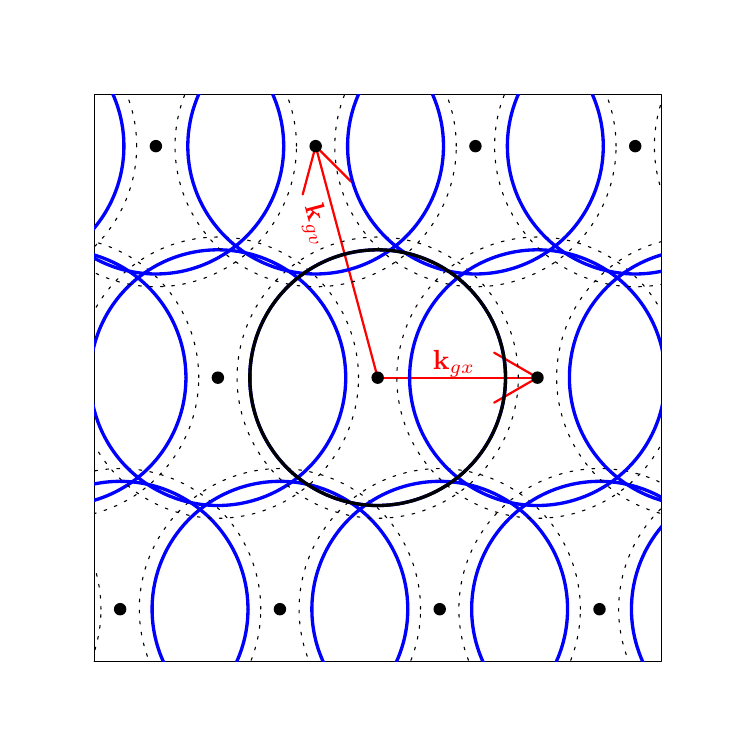
\begin{tikzpicture}[x=1pt,y=1pt]
\definecolor[named]{fillColor}{rgb}{1.00,1.00,1.00}
\path[use as bounding box,fill=fillColor,fill opacity=0.00] (0,0) rectangle (252.94,252.94);
\begin{scope}
\path[clip] (  0.00,  0.00) rectangle (252.94,252.94);
\definecolor[named]{drawColor}{rgb}{0.00,0.00,0.00}

\path[draw=drawColor,line width= 0.4pt,line join=round,line cap=round] ( 24.00, 24.00) --
	(228.94, 24.00) --
	(228.94,228.94) --
	( 24.00,228.94) --
	( 24.00, 24.00);
\end{scope}
\begin{scope}
\path[clip] ( 24.00, 24.00) rectangle (228.94,228.94);
\definecolor[named]{drawColor}{rgb}{0.00,0.00,0.00}

\path[draw=drawColor,line width= 0.4pt,line join=round,line cap=round] (126.47,126.47) --
	(126.47,126.47);
\definecolor[named]{drawColor}{rgb}{1.00,0.00,0.00}
\definecolor[named]{fillColor}{rgb}{1.00,1.00,1.00}

\path[draw=drawColor,line width= 0.8pt,line join=round,line cap=round,fill=fillColor] (126.47,126.47) -- (184.21,126.47);

\path[draw=drawColor,line width= 0.8pt,line join=round,line cap=round] (168.57,117.44) --
	(184.21,126.47) --
	(168.57,135.51);

\path[draw=drawColor,line width= 0.8pt,line join=round,line cap=round,fill=fillColor] (126.47,126.47) -- (104.06,210.13);

\path[draw=drawColor,line width= 0.8pt,line join=round,line cap=round] (116.83,197.36) --
	(104.06,210.13) --
	( 99.38,192.68);
\definecolor[named]{drawColor}{rgb}{0.00,0.00,1.00}

\path[draw=drawColor,line width= 1.2pt,line join=round,line cap=round] ( 19.66,  0.00) --
	( 19.65,  0.01) --
	( 18.93,  0.38) --
	( 18.20,  0.74) --
	( 17.47,  1.08) --
	( 16.74,  1.41) --
	( 15.99,  1.73) --
	( 15.25,  2.04) --
	( 14.49,  2.33) --
	( 13.74,  2.62) --
	( 12.97,  2.88) --
	( 12.20,  3.14) --
	( 11.43,  3.38) --
	( 10.66,  3.60) --
	(  9.88,  3.82) --
	(  9.09,  4.02) --
	(  8.31,  4.20) --
	(  7.52,  4.37) --
	(  6.72,  4.53) --
	(  5.93,  4.68) --
	(  5.13,  4.81) --
	(  4.33,  4.92) --
	(  3.53,  5.03) --
	(  2.72,  5.11) --
	(  1.92,  5.19) --
	(  1.11,  5.25) --
	(  0.31,  5.29) --
	(  0.00,  5.31);
\definecolor[named]{drawColor}{rgb}{0.00,0.00,0.00}

\path[draw=drawColor,line width= 0.4pt,dash pattern=on 1pt off 3pt ,line join=round,line cap=round] ( 28.31,  0.00) --
	( 27.84,  0.34) --
	( 27.12,  0.86) --
	( 26.38,  1.36) --
	( 25.64,  1.85) --
	( 24.89,  2.32) --
	( 24.13,  2.78) --
	( 23.36,  3.23) --
	( 22.59,  3.67) --
	( 21.80,  4.09) --
	( 21.01,  4.50) --
	( 20.22,  4.89) --
	( 19.41,  5.27) --
	( 18.60,  5.64) --
	( 17.79,  5.99) --
	( 16.96,  6.33) --
	( 16.13,  6.65) --
	( 15.30,  6.96) --
	( 14.46,  7.26) --
	( 13.62,  7.53) --
	( 12.77,  7.80) --
	( 11.91,  8.05) --
	( 11.06,  8.28) --
	( 10.19,  8.50) --
	(  9.33,  8.71) --
	(  8.46,  8.90) --
	(  7.59,  9.07) --
	(  6.71,  9.23) --
	(  5.83,  9.37) --
	(  4.95,  9.50) --
	(  4.07,  9.61) --
	(  3.19,  9.71) --
	(  2.30,  9.79) --
	(  1.42,  9.86) --
	(  0.53,  9.91) --
	(  0.00,  9.93);
\definecolor[named]{drawColor}{rgb}{0.00,0.00,1.00}

\path[draw=drawColor,line width= 1.2pt,line join=round,line cap=round] ( 21.86, 42.81) --
	( 21.85, 43.62) --
	( 21.83, 44.43) --
	( 21.80, 45.24) --
	( 21.75, 46.04) --
	( 21.68, 46.85) --
	( 21.61, 47.65) --
	( 21.52, 48.46) --
	( 21.41, 49.26) --
	( 21.29, 50.06) --
	( 21.16, 50.86) --
	( 21.01, 51.65) --
	( 20.85, 52.44) --
	( 20.67, 53.23) --
	( 20.48, 54.02) --
	( 20.28, 54.80) --
	( 20.06, 55.58) --
	( 19.83, 56.36) --
	( 19.59, 57.13) --
	( 19.33, 57.89) --
	( 19.06, 58.65) --
	( 18.78, 59.41) --
	( 18.48, 60.16) --
	( 18.17, 60.91) --
	( 17.85, 61.65) --
	( 17.51, 62.39) --
	( 17.16, 63.12) --
	( 16.80, 63.84) --
	( 16.42, 64.56) --
	( 16.04, 65.27) --
	( 15.64, 65.97) --
	( 15.23, 66.66) --
	( 14.80, 67.35) --
	( 14.37, 68.03) --
	( 13.92, 68.71) --
	( 13.46, 69.37) --
	( 12.99, 70.03) --
	( 12.51, 70.68) --
	( 12.02, 71.32) --
	( 11.51, 71.95) --
	( 11.00, 72.57) --
	( 10.47, 73.19) --
	(  9.93, 73.79) --
	(  9.39, 74.39) --
	(  8.83, 74.97) --
	(  8.26, 75.55) --
	(  7.68, 76.11) --
	(  7.09, 76.67) --
	(  6.50, 77.21) --
	(  5.89, 77.75) --
	(  5.27, 78.27) --
	(  4.65, 78.78) --
	(  4.02, 79.29) --
	(  3.37, 79.78) --
	(  2.72, 80.26) --
	(  2.06, 80.72) --
	(  1.39, 81.18) --
	(  0.72, 81.62) --
	(  0.04, 82.06) --
	(  0.00, 82.08);

\path[draw=drawColor,line width= 1.2pt,line join=round,line cap=round] (  0.00,  3.55) --
	(  0.04,  3.57) --
	(  0.72,  4.00) --
	(  1.39,  4.44) --
	(  2.06,  4.90) --
	(  2.72,  5.37) --
	(  3.37,  5.85) --
	(  4.02,  6.34) --
	(  4.65,  6.84) --
	(  5.27,  7.35) --
	(  5.89,  7.88) --
	(  6.50,  8.41) --
	(  7.09,  8.96) --
	(  7.68,  9.51) --
	(  8.26, 10.08) --
	(  8.83, 10.65) --
	(  9.39, 11.24) --
	(  9.93, 11.83) --
	( 10.47, 12.44) --
	( 11.00, 13.05) --
	( 11.51, 13.67) --
	( 12.02, 14.30) --
	( 12.51, 14.95) --
	( 12.99, 15.59) --
	( 13.46, 16.25) --
	( 13.92, 16.92) --
	( 14.37, 17.59) --
	( 14.80, 18.27) --
	( 15.23, 18.96) --
	( 15.64, 19.66) --
	( 16.04, 20.36) --
	( 16.42, 21.07) --
	( 16.80, 21.79) --
	( 17.16, 22.51) --
	( 17.51, 23.24) --
	( 17.85, 23.97) --
	( 18.17, 24.72) --
	( 18.48, 25.46) --
	( 18.78, 26.21) --
	( 19.06, 26.97) --
	( 19.33, 27.73) --
	( 19.59, 28.50) --
	( 19.83, 29.27) --
	( 20.06, 30.04) --
	( 20.28, 30.82) --
	( 20.48, 31.61) --
	( 20.67, 32.39) --
	( 20.85, 33.18) --
	( 21.01, 33.97) --
	( 21.16, 34.77) --
	( 21.29, 35.57) --
	( 21.41, 36.37) --
	( 21.52, 37.17) --
	( 21.61, 37.97) --
	( 21.68, 38.78) --
	( 21.75, 39.58) --
	( 21.80, 40.39) --
	( 21.83, 41.20) --
	( 21.85, 42.00) --
	( 21.86, 42.81);
\definecolor[named]{drawColor}{rgb}{0.00,0.00,0.00}

\path[draw=drawColor,line width= 0.4pt,dash pattern=on 1pt off 3pt ,line join=round,line cap=round] ( 26.48, 42.81) --
	( 26.47, 43.70) --
	( 26.45, 44.59) --
	( 26.41, 45.48) --
	( 26.36, 46.37) --
	( 26.29, 47.25) --
	( 26.20, 48.14) --
	( 26.10, 49.02) --
	( 25.98, 49.90) --
	( 25.85, 50.78) --
	( 25.70, 51.66) --
	( 25.54, 52.54) --
	( 25.36, 53.41) --
	( 25.17, 54.27) --
	( 24.96, 55.14) --
	( 24.74, 56.00) --
	( 24.50, 56.86) --
	( 24.25, 57.71) --
	( 23.98, 58.56) --
	( 23.70, 59.40) --
	( 23.40, 60.24) --
	( 23.09, 61.07) --
	( 22.76, 61.90) --
	( 22.42, 62.72) --
	( 22.06, 63.53) --
	( 21.69, 64.34) --
	( 21.31, 65.15) --
	( 20.91, 65.94) --
	( 20.50, 66.73) --
	( 20.08, 67.51) --
	( 19.64, 68.28) --
	( 19.18, 69.05) --
	( 18.72, 69.81) --
	( 18.24, 70.56) --
	( 17.75, 71.30) --
	( 17.24, 72.03) --
	( 16.72, 72.75) --
	( 16.19, 73.47) --
	( 15.65, 74.17) --
	( 15.10, 74.87) --
	( 14.53, 75.55) --
	( 13.95, 76.23) --
	( 13.36, 76.89) --
	( 12.76, 77.55) --
	( 12.14, 78.19) --
	( 11.52, 78.82) --
	( 10.88, 79.44) --
	( 10.24, 80.05) --
	(  9.58, 80.65) --
	(  8.91, 81.24) --
	(  8.23, 81.82) --
	(  7.55, 82.38) --
	(  6.85, 82.93) --
	(  6.14, 83.47) --
	(  5.43, 84.00) --
	(  4.70, 84.52) --
	(  3.97, 85.02) --
	(  3.22, 85.51) --
	(  2.47, 85.98) --
	(  1.71, 86.44) --
	(  0.95, 86.89) --
	(  0.17, 87.33) --
	(  0.00, 87.42);

\path[draw=drawColor,line width= 0.4pt,dash pattern=on 1pt off 3pt ,line join=round,line cap=round] (  3.04,  0.00) --
	(  3.22,  0.12) --
	(  3.97,  0.61) --
	(  4.70,  1.11) --
	(  5.43,  1.62) --
	(  6.14,  2.15) --
	(  6.85,  2.69) --
	(  7.55,  3.24) --
	(  8.23,  3.81) --
	(  8.91,  4.38) --
	(  9.58,  4.97) --
	( 10.24,  5.57) --
	( 10.88,  6.18) --
	( 11.52,  6.80) --
	( 12.14,  7.44) --
	( 12.76,  8.08) --
	( 13.36,  8.73) --
	( 13.95,  9.40) --
	( 14.53, 10.07) --
	( 15.10, 10.76) --
	( 15.65, 11.45) --
	( 16.19, 12.16) --
	( 16.72, 12.87) --
	( 17.24, 13.60) --
	( 17.75, 14.33) --
	( 18.24, 15.07) --
	( 18.72, 15.82) --
	( 19.18, 16.58) --
	( 19.64, 17.34) --
	( 20.08, 18.11) --
	( 20.50, 18.90) --
	( 20.91, 19.68) --
	( 21.31, 20.48) --
	( 21.69, 21.28) --
	( 22.06, 22.09) --
	( 22.42, 22.91) --
	( 22.76, 23.73) --
	( 23.09, 24.55) --
	( 23.40, 25.39) --
	( 23.70, 26.22) --
	( 23.98, 27.07) --
	( 24.25, 27.92) --
	( 24.50, 28.77) --
	( 24.74, 29.62) --
	( 24.96, 30.49) --
	( 25.17, 31.35) --
	( 25.36, 32.22) --
	( 25.54, 33.09) --
	( 25.70, 33.96) --
	( 25.85, 34.84) --
	( 25.98, 35.72) --
	( 26.10, 36.60) --
	( 26.20, 37.49) --
	( 26.29, 38.37) --
	( 26.36, 39.26) --
	( 26.41, 40.15) --
	( 26.45, 41.03) --
	( 26.47, 41.92) --
	( 26.48, 42.81);

\path[draw=drawColor,line width= 0.4pt,dash pattern=on 1pt off 3pt ,line join=round,line cap=round] (  4.06,126.47) --
	(  4.06,127.36) --
	(  4.03,128.25) --
	(  3.99,129.14) --
	(  3.94,130.03) --
	(  3.87,130.91) --
	(  3.78,131.80) --
	(  3.68,132.68) --
	(  3.57,133.56) --
	(  3.44,134.44) --
	(  3.29,135.32) --
	(  3.13,136.20) --
	(  2.95,137.07) --
	(  2.75,137.93) --
	(  2.55,138.80) --
	(  2.32,139.66) --
	(  2.09,140.52) --
	(  1.83,141.37) --
	(  1.56,142.22) --
	(  1.28,143.06) --
	(  0.98,143.90) --
	(  0.67,144.73) --
	(  0.34,145.56) --
	(  0.00,146.38) --
	(  0.00,146.39);

\path[draw=drawColor,line width= 0.4pt,dash pattern=on 1pt off 3pt ,line join=round,line cap=round] (  0.00,106.56) --
	(  0.00,106.57) --
	(  0.34,107.39) --
	(  0.67,108.21) --
	(  0.98,109.05) --
	(  1.28,109.88) --
	(  1.56,110.73) --
	(  1.83,111.58) --
	(  2.09,112.43) --
	(  2.32,113.28) --
	(  2.55,114.15) --
	(  2.75,115.01) --
	(  2.95,115.88) --
	(  3.13,116.75) --
	(  3.29,117.62) --
	(  3.44,118.50) --
	(  3.57,119.38) --
	(  3.68,120.26) --
	(  3.78,121.15) --
	(  3.87,122.03) --
	(  3.94,122.92) --
	(  3.99,123.81) --
	(  4.03,124.69) --
	(  4.06,125.58) --
	(  4.06,126.47);
\definecolor[named]{drawColor}{rgb}{0.00,0.00,1.00}

\path[draw=drawColor,line width= 1.2pt,line join=round,line cap=round] ( 77.40,  0.00) --
	( 77.39,  0.01) --
	( 76.67,  0.38) --
	( 75.95,  0.74) --
	( 75.21,  1.08) --
	( 74.48,  1.41) --
	( 73.74,  1.73) --
	( 72.99,  2.04) --
	( 72.23,  2.33) --
	( 71.48,  2.62) --
	( 70.71,  2.88) --
	( 69.95,  3.14) --
	( 69.17,  3.38) --
	( 68.40,  3.60) --
	( 67.62,  3.82) --
	( 66.83,  4.02) --
	( 66.05,  4.20) --
	( 65.26,  4.37) --
	( 64.46,  4.53) --
	( 63.67,  4.68) --
	( 62.87,  4.81) --
	( 62.07,  4.92) --
	( 61.27,  5.03) --
	( 60.47,  5.11) --
	( 59.66,  5.19) --
	( 58.85,  5.25) --
	( 58.05,  5.29) --
	( 57.24,  5.33) --
	( 56.43,  5.34) --
	( 55.62,  5.35) --
	( 54.81,  5.34) --
	( 54.01,  5.31) --
	( 53.20,  5.27) --
	( 52.39,  5.22) --
	( 51.59,  5.15) --
	( 50.78,  5.07) --
	( 49.98,  4.98) --
	( 49.18,  4.87) --
	( 48.38,  4.74) --
	( 47.58,  4.61) --
	( 46.79,  4.45) --
	( 46.00,  4.29) --
	( 45.21,  4.11) --
	( 44.42,  3.92) --
	( 43.64,  3.71) --
	( 42.86,  3.49) --
	( 42.09,  3.26) --
	( 41.32,  3.01) --
	( 40.55,  2.75) --
	( 39.79,  2.48) --
	( 39.04,  2.19) --
	( 38.29,  1.89) --
	( 37.54,  1.58) --
	( 36.80,  1.25) --
	( 36.07,  0.91) --
	( 35.34,  0.56) --
	( 34.62,  0.19) --
	( 34.25,  0.00);
\definecolor[named]{drawColor}{rgb}{0.00,0.00,0.00}

\path[draw=drawColor,line width= 0.4pt,dash pattern=on 1pt off 3pt ,line join=round,line cap=round] ( 86.05,  0.00) --
	( 85.58,  0.34) --
	( 84.86,  0.86) --
	( 84.12,  1.36) --
	( 83.38,  1.85) --
	( 82.63,  2.32) --
	( 81.87,  2.78) --
	( 81.10,  3.23) --
	( 80.33,  3.67) --
	( 79.54,  4.09) --
	( 78.75,  4.50) --
	( 77.96,  4.89) --
	( 77.15,  5.27) --
	( 76.34,  5.64) --
	( 75.53,  5.99) --
	( 74.70,  6.33) --
	( 73.88,  6.65) --
	( 73.04,  6.96) --
	( 72.20,  7.26) --
	( 71.36,  7.53) --
	( 70.51,  7.80) --
	( 69.65,  8.05) --
	( 68.80,  8.28) --
	( 67.94,  8.50) --
	( 67.07,  8.71) --
	( 66.20,  8.90) --
	( 65.33,  9.07) --
	( 64.45,  9.23) --
	( 63.58,  9.37) --
	( 62.70,  9.50) --
	( 61.81,  9.61) --
	( 60.93,  9.71) --
	( 60.04,  9.79) --
	( 59.16,  9.86) --
	( 58.27,  9.91) --
	( 57.38,  9.94) --
	( 56.49,  9.96) --
	( 55.60,  9.97) --
	( 54.71,  9.95) --
	( 53.82,  9.93) --
	( 52.94,  9.88) --
	( 52.05,  9.83) --
	( 51.16,  9.75) --
	( 50.28,  9.66) --
	( 49.39,  9.56) --
	( 48.51,  9.44) --
	( 47.63,  9.30) --
	( 46.76,  9.15) --
	( 45.88,  8.99) --
	( 45.01,  8.80) --
	( 44.15,  8.61) --
	( 43.28,  8.39) --
	( 42.42,  8.17) --
	( 41.57,  7.93) --
	( 40.71,  7.67) --
	( 39.87,  7.40) --
	( 39.03,  7.11) --
	( 38.19,  6.81) --
	( 37.36,  6.49) --
	( 36.53,  6.16) --
	( 35.71,  5.82) --
	( 34.90,  5.46) --
	( 34.09,  5.09) --
	( 33.29,  4.70) --
	( 32.50,  4.30) --
	( 31.71,  3.88) --
	( 30.93,  3.45) --
	( 30.16,  3.01) --
	( 29.40,  2.55) --
	( 28.64,  2.09) --
	( 27.89,  1.60) --
	( 27.16,  1.11) --
	( 26.43,  0.60) --
	( 25.70,  0.08) --
	( 25.60,  0.00);
\definecolor[named]{fillColor}{rgb}{0.00,0.00,0.00}

\path[fill=fillColor] ( 33.41, 42.81) circle (  2.25);
\definecolor[named]{drawColor}{rgb}{0.00,0.00,1.00}

\path[draw=drawColor,line width= 1.2pt,line join=round,line cap=round] ( 79.60, 42.81) --
	( 79.60, 43.62) --
	( 79.57, 44.43) --
	( 79.54, 45.24) --
	( 79.49, 46.04) --
	( 79.43, 46.85) --
	( 79.35, 47.65) --
	( 79.26, 48.46) --
	( 79.15, 49.26) --
	( 79.03, 50.06) --
	( 78.90, 50.86) --
	( 78.75, 51.65) --
	( 78.59, 52.44) --
	( 78.41, 53.23) --
	( 78.22, 54.02) --
	( 78.02, 54.80) --
	( 77.80, 55.58) --
	( 77.57, 56.36) --
	( 77.33, 57.13) --
	( 77.07, 57.89) --
	( 76.80, 58.65) --
	( 76.52, 59.41) --
	( 76.22, 60.16) --
	( 75.91, 60.91) --
	( 75.59, 61.65) --
	( 75.25, 62.39) --
	( 74.90, 63.12) --
	( 74.54, 63.84) --
	( 74.17, 64.56) --
	( 73.78, 65.27) --
	( 73.38, 65.97) --
	( 72.97, 66.66) --
	( 72.54, 67.35) --
	( 72.11, 68.03) --
	( 71.66, 68.71) --
	( 71.20, 69.37) --
	( 70.73, 70.03) --
	( 70.25, 70.68) --
	( 69.76, 71.32) --
	( 69.25, 71.95) --
	( 68.74, 72.57) --
	( 68.21, 73.19) --
	( 67.67, 73.79) --
	( 67.13, 74.39) --
	( 66.57, 74.97) --
	( 66.00, 75.55) --
	( 65.42, 76.11) --
	( 64.84, 76.67) --
	( 64.24, 77.21) --
	( 63.63, 77.75) --
	( 63.01, 78.27) --
	( 62.39, 78.78) --
	( 61.76, 79.29) --
	( 61.11, 79.78) --
	( 60.46, 80.26) --
	( 59.80, 80.72) --
	( 59.14, 81.18) --
	( 58.46, 81.62) --
	( 57.78, 82.06) --
	( 57.09, 82.48) --
	( 56.39, 82.89) --
	( 55.68, 83.28) --
	( 54.97, 83.67) --
	( 54.25, 84.04) --
	( 53.53, 84.40) --
	( 52.80, 84.74) --
	( 52.06, 85.07) --
	( 51.32, 85.39) --
	( 50.57, 85.70) --
	( 49.82, 85.99) --
	( 49.06, 86.28) --
	( 48.30, 86.54) --
	( 47.53, 86.80) --
	( 46.76, 87.04) --
	( 45.98, 87.26) --
	( 45.20, 87.48) --
	( 44.42, 87.68) --
	( 43.63, 87.86) --
	( 42.84, 88.03) --
	( 42.05, 88.19) --
	( 41.25, 88.34) --
	( 40.45, 88.47) --
	( 39.65, 88.58) --
	( 38.85, 88.69) --
	( 38.05, 88.77) --
	( 37.24, 88.85) --
	( 36.44, 88.91) --
	( 35.63, 88.95) --
	( 34.82, 88.99) --
	( 34.01, 89.00) --
	( 33.21, 89.01) --
	( 32.40, 89.00) --
	( 31.59, 88.97) --
	( 30.78, 88.93) --
	( 29.97, 88.88) --
	( 29.17, 88.81) --
	( 28.36, 88.73) --
	( 27.56, 88.64) --
	( 26.76, 88.53) --
	( 25.96, 88.40) --
	( 25.16, 88.27) --
	( 24.37, 88.11) --
	( 23.58, 87.95) --
	( 22.79, 87.77) --
	( 22.01, 87.58) --
	( 21.22, 87.37) --
	( 20.45, 87.15) --
	( 19.67, 86.92) --
	( 18.90, 86.67) --
	( 18.14, 86.41) --
	( 17.38, 86.14) --
	( 16.62, 85.85) --
	( 15.87, 85.55) --
	( 15.12, 85.24) --
	( 14.38, 84.91) --
	( 13.65, 84.57) --
	( 12.92, 84.22) --
	( 12.20, 83.85) --
	( 11.49, 83.48) --
	( 10.78, 83.09) --
	( 10.08, 82.68) --
	(  9.38, 82.27) --
	(  8.70, 81.84) --
	(  8.02, 81.40) --
	(  7.35, 80.95) --
	(  6.68, 80.49) --
	(  6.03, 80.02) --
	(  5.38, 79.53) --
	(  4.74, 79.04) --
	(  4.11, 78.53) --
	(  3.49, 78.01) --
	(  2.88, 77.48) --
	(  2.28, 76.94) --
	(  1.68, 76.39) --
	(  1.10, 75.83) --
	(  0.53, 75.26) --
	(  0.00, 74.72);

\path[draw=drawColor,line width= 1.2pt,line join=round,line cap=round] (  0.00, 10.91) --
	(  0.53, 10.36) --
	(  1.10,  9.79) --
	(  1.68,  9.23) --
	(  2.28,  8.68) --
	(  2.88,  8.14) --
	(  3.49,  7.61) --
	(  4.11,  7.10) --
	(  4.74,  6.59) --
	(  5.38,  6.09) --
	(  6.03,  5.61) --
	(  6.68,  5.13) --
	(  7.35,  4.67) --
	(  8.02,  4.22) --
	(  8.70,  3.78) --
	(  9.38,  3.36) --
	( 10.08,  2.94) --
	( 10.78,  2.54) --
	( 11.49,  2.15) --
	( 12.20,  1.77) --
	( 12.92,  1.41) --
	( 13.65,  1.06) --
	( 14.38,  0.72) --
	( 15.12,  0.39) --
	( 15.87,  0.08) --
	( 16.06,  0.00);

\path[draw=drawColor,line width= 1.2pt,line join=round,line cap=round] ( 50.76,  0.00) --
	( 51.32,  0.23) --
	( 52.06,  0.55) --
	( 52.80,  0.88) --
	( 53.53,  1.23) --
	( 54.25,  1.59) --
	( 54.97,  1.96) --
	( 55.68,  2.34) --
	( 56.39,  2.74) --
	( 57.09,  3.15) --
	( 57.78,  3.57) --
	( 58.46,  4.00) --
	( 59.14,  4.44) --
	( 59.80,  4.90) --
	( 60.46,  5.37) --
	( 61.11,  5.85) --
	( 61.76,  6.34) --
	( 62.39,  6.84) --
	( 63.01,  7.35) --
	( 63.63,  7.88) --
	( 64.24,  8.41) --
	( 64.84,  8.96) --
	( 65.42,  9.51) --
	( 66.00, 10.08) --
	( 66.57, 10.65) --
	( 67.13, 11.24) --
	( 67.67, 11.83) --
	( 68.21, 12.44) --
	( 68.74, 13.05) --
	( 69.25, 13.67) --
	( 69.76, 14.30) --
	( 70.25, 14.95) --
	( 70.73, 15.59) --
	( 71.20, 16.25) --
	( 71.66, 16.92) --
	( 72.11, 17.59) --
	( 72.54, 18.27) --
	( 72.97, 18.96) --
	( 73.38, 19.66) --
	( 73.78, 20.36) --
	( 74.17, 21.07) --
	( 74.54, 21.79) --
	( 74.90, 22.51) --
	( 75.25, 23.24) --
	( 75.59, 23.97) --
	( 75.91, 24.72) --
	( 76.22, 25.46) --
	( 76.52, 26.21) --
	( 76.80, 26.97) --
	( 77.07, 27.73) --
	( 77.33, 28.50) --
	( 77.57, 29.27) --
	( 77.80, 30.04) --
	( 78.02, 30.82) --
	( 78.22, 31.61) --
	( 78.41, 32.39) --
	( 78.59, 33.18) --
	( 78.75, 33.97) --
	( 78.90, 34.77) --
	( 79.03, 35.57) --
	( 79.15, 36.37) --
	( 79.26, 37.17) --
	( 79.35, 37.97) --
	( 79.43, 38.78) --
	( 79.49, 39.58) --
	( 79.54, 40.39) --
	( 79.57, 41.20) --
	( 79.60, 42.00) --
	( 79.60, 42.81);
\definecolor[named]{drawColor}{rgb}{0.00,0.00,0.00}

\path[draw=drawColor,line width= 0.4pt,dash pattern=on 1pt off 3pt ,line join=round,line cap=round] ( 84.22, 42.81) --
	( 84.21, 43.70) --
	( 84.19, 44.59) --
	( 84.15, 45.48) --
	( 84.10, 46.37) --
	( 84.03, 47.25) --
	( 83.94, 48.14) --
	( 83.84, 49.02) --
	( 83.72, 49.90) --
	( 83.59, 50.78) --
	( 83.45, 51.66) --
	( 83.28, 52.54) --
	( 83.11, 53.41) --
	( 82.91, 54.27) --
	( 82.70, 55.14) --
	( 82.48, 56.00) --
	( 82.24, 56.86) --
	( 81.99, 57.71) --
	( 81.72, 58.56) --
	( 81.44, 59.40) --
	( 81.14, 60.24) --
	( 80.83, 61.07) --
	( 80.50, 61.90) --
	( 80.16, 62.72) --
	( 79.80, 63.53) --
	( 79.43, 64.34) --
	( 79.05, 65.15) --
	( 78.65, 65.94) --
	( 78.24, 66.73) --
	( 77.82, 67.51) --
	( 77.38, 68.28) --
	( 76.92, 69.05) --
	( 76.46, 69.81) --
	( 75.98, 70.56) --
	( 75.49, 71.30) --
	( 74.98, 72.03) --
	( 74.46, 72.75) --
	( 73.93, 73.47) --
	( 73.39, 74.17) --
	( 72.84, 74.87) --
	( 72.27, 75.55) --
	( 71.69, 76.23) --
	( 71.10, 76.89) --
	( 70.50, 77.55) --
	( 69.88, 78.19) --
	( 69.26, 78.82) --
	( 68.62, 79.44) --
	( 67.98, 80.05) --
	( 67.32, 80.65) --
	( 66.65, 81.24) --
	( 65.98, 81.82) --
	( 65.29, 82.38) --
	( 64.59, 82.93) --
	( 63.88, 83.47) --
	( 63.17, 84.00) --
	( 62.44, 84.52) --
	( 61.71, 85.02) --
	( 60.96, 85.51) --
	( 60.21, 85.98) --
	( 59.45, 86.44) --
	( 58.69, 86.89) --
	( 57.91, 87.33) --
	( 57.13, 87.75) --
	( 56.34, 88.16) --
	( 55.54, 88.55) --
	( 54.74, 88.93) --
	( 53.93, 89.30) --
	( 53.11, 89.65) --
	( 52.29, 89.99) --
	( 51.46, 90.31) --
	( 50.62, 90.62) --
	( 49.79, 90.92) --
	( 48.94, 91.19) --
	( 48.09, 91.46) --
	( 47.24, 91.71) --
	( 46.38, 91.94) --
	( 45.52, 92.16) --
	( 44.65, 92.37) --
	( 43.78, 92.56) --
	( 42.91, 92.73) --
	( 42.04, 92.89) --
	( 41.16, 93.03) --
	( 40.28, 93.16) --
	( 39.40, 93.27) --
	( 38.51, 93.37) --
	( 37.63, 93.45) --
	( 36.74, 93.52) --
	( 35.85, 93.57) --
	( 34.96, 93.60) --
	( 34.07, 93.62) --
	( 33.19, 93.63) --
	( 32.30, 93.61) --
	( 31.41, 93.59) --
	( 30.52, 93.54) --
	( 29.63, 93.49) --
	( 28.75, 93.41) --
	( 27.86, 93.32) --
	( 26.98, 93.22) --
	( 26.10, 93.10) --
	( 25.22, 92.96) --
	( 24.34, 92.81) --
	( 23.47, 92.65) --
	( 22.60, 92.46) --
	( 21.73, 92.27) --
	( 20.87, 92.05) --
	( 20.01, 91.83) --
	( 19.15, 91.59) --
	( 18.30, 91.33) --
	( 17.45, 91.06) --
	( 16.61, 90.77) --
	( 15.77, 90.47) --
	( 14.94, 90.15) --
	( 14.12, 89.82) --
	( 13.30, 89.48) --
	( 12.48, 89.12) --
	( 11.68, 88.75) --
	( 10.87, 88.36) --
	( 10.08, 87.96) --
	(  9.29, 87.54) --
	(  8.52, 87.11) --
	(  7.74, 86.67) --
	(  6.98, 86.21) --
	(  6.22, 85.75) --
	(  5.48, 85.26) --
	(  4.74, 84.77) --
	(  4.01, 84.26) --
	(  3.29, 83.74) --
	(  2.58, 83.21) --
	(  1.87, 82.66) --
	(  1.18, 82.10) --
	(  0.50, 81.53) --
	(  0.00, 81.10);

\path[draw=drawColor,line width= 0.4pt,dash pattern=on 1pt off 3pt ,line join=round,line cap=round] (  0.00,  4.53) --
	(  0.50,  4.09) --
	(  1.18,  3.52) --
	(  1.87,  2.97) --
	(  2.58,  2.42) --
	(  3.29,  1.89) --
	(  4.01,  1.37) --
	(  4.74,  0.86) --
	(  5.48,  0.36) --
	(  6.04,  0.00);

\path[draw=drawColor,line width= 0.4pt,dash pattern=on 1pt off 3pt ,line join=round,line cap=round] ( 60.78,  0.00) --
	( 60.96,  0.12) --
	( 61.71,  0.61) --
	( 62.44,  1.11) --
	( 63.17,  1.62) --
	( 63.88,  2.15) --
	( 64.59,  2.69) --
	( 65.29,  3.24) --
	( 65.98,  3.81) --
	( 66.65,  4.38) --
	( 67.32,  4.97) --
	( 67.98,  5.57) --
	( 68.62,  6.18) --
	( 69.26,  6.80) --
	( 69.88,  7.44) --
	( 70.50,  8.08) --
	( 71.10,  8.73) --
	( 71.69,  9.40) --
	( 72.27, 10.07) --
	( 72.84, 10.76) --
	( 73.39, 11.45) --
	( 73.93, 12.16) --
	( 74.46, 12.87) --
	( 74.98, 13.60) --
	( 75.49, 14.33) --
	( 75.98, 15.07) --
	( 76.46, 15.82) --
	( 76.92, 16.58) --
	( 77.38, 17.34) --
	( 77.82, 18.11) --
	( 78.24, 18.90) --
	( 78.65, 19.68) --
	( 79.05, 20.48) --
	( 79.43, 21.28) --
	( 79.80, 22.09) --
	( 80.16, 22.91) --
	( 80.50, 23.73) --
	( 80.83, 24.55) --
	( 81.14, 25.39) --
	( 81.44, 26.22) --
	( 81.72, 27.07) --
	( 81.99, 27.92) --
	( 82.24, 28.77) --
	( 82.48, 29.62) --
	( 82.70, 30.49) --
	( 82.91, 31.35) --
	( 83.11, 32.22) --
	( 83.28, 33.09) --
	( 83.45, 33.96) --
	( 83.59, 34.84) --
	( 83.72, 35.72) --
	( 83.84, 36.60) --
	( 83.94, 37.49) --
	( 84.03, 38.37) --
	( 84.10, 39.26) --
	( 84.15, 40.15) --
	( 84.19, 41.03) --
	( 84.21, 41.92) --
	( 84.22, 42.81);

\path[fill=fillColor] ( 10.99,126.47) circle (  2.25);
\definecolor[named]{drawColor}{rgb}{0.00,0.00,1.00}

\path[draw=drawColor,line width= 1.2pt,line join=round,line cap=round] ( 57.19,126.47) --
	( 57.18,127.28) --
	( 57.16,128.09) --
	( 57.12,128.90) --
	( 57.07,129.70) --
	( 57.01,130.51) --
	( 56.93,131.31) --
	( 56.84,132.12) --
	( 56.73,132.92) --
	( 56.61,133.72) --
	( 56.48,134.52) --
	( 56.33,135.31) --
	( 56.17,136.10) --
	( 56.00,136.89) --
	( 55.81,137.68) --
	( 55.60,138.46) --
	( 55.39,139.24) --
	( 55.16,140.02) --
	( 54.91,140.79) --
	( 54.66,141.55) --
	( 54.38,142.31) --
	( 54.10,143.07) --
	( 53.80,143.82) --
	( 53.49,144.57) --
	( 53.17,145.31) --
	( 52.83,146.05) --
	( 52.49,146.78) --
	( 52.12,147.50) --
	( 51.75,148.22) --
	( 51.36,148.93) --
	( 50.96,149.63) --
	( 50.55,150.32) --
	( 50.13,151.01) --
	( 49.69,151.69) --
	( 49.25,152.37) --
	( 48.79,153.03) --
	( 48.32,153.69) --
	( 47.83,154.34) --
	( 47.34,154.98) --
	( 46.84,155.61) --
	( 46.32,156.23) --
	( 45.79,156.85) --
	( 45.26,157.45) --
	( 44.71,158.05) --
	( 44.15,158.63) --
	( 43.58,159.21) --
	( 43.01,159.77) --
	( 42.42,160.33) --
	( 41.82,160.87) --
	( 41.21,161.41) --
	( 40.60,161.93) --
	( 39.97,162.44) --
	( 39.34,162.95) --
	( 38.70,163.44) --
	( 38.05,163.92) --
	( 37.39,164.38) --
	( 36.72,164.84) --
	( 36.04,165.28) --
	( 35.36,165.72) --
	( 34.67,166.14) --
	( 33.97,166.55) --
	( 33.27,166.94) --
	( 32.56,167.33) --
	( 31.84,167.70) --
	( 31.11,168.06) --
	( 30.38,168.40) --
	( 29.64,168.73) --
	( 28.90,169.05) --
	( 28.15,169.36) --
	( 27.40,169.65) --
	( 26.64,169.94) --
	( 25.88,170.20) --
	( 25.11,170.46) --
	( 24.34,170.70) --
	( 23.56,170.92) --
	( 22.78,171.14) --
	( 22.00,171.34) --
	( 21.21,171.52) --
	( 20.42,171.69) --
	( 19.63,171.85) --
	( 18.84,172.00) --
	( 18.04,172.13) --
	( 17.24,172.24) --
	( 16.44,172.35) --
	( 15.63,172.43) --
	( 14.83,172.51) --
	( 14.02,172.57) --
	( 13.21,172.61) --
	( 12.41,172.65) --
	( 11.60,172.66) --
	( 10.79,172.67) --
	(  9.98,172.66) --
	(  9.17,172.63) --
	(  8.36,172.59) --
	(  7.56,172.54) --
	(  6.75,172.47) --
	(  5.95,172.39) --
	(  5.15,172.30) --
	(  4.34,172.19) --
	(  3.54,172.06) --
	(  2.75,171.93) --
	(  1.95,171.77) --
	(  1.16,171.61) --
	(  0.37,171.43) --
	(  0.00,171.34);

\path[draw=drawColor,line width= 1.2pt,line join=round,line cap=round] (  0.00, 81.61) --
	(  0.37, 81.51) --
	(  1.16, 81.34) --
	(  1.95, 81.17) --
	(  2.75, 81.02) --
	(  3.54, 80.88) --
	(  4.34, 80.76) --
	(  5.15, 80.65) --
	(  5.95, 80.55) --
	(  6.75, 80.47) --
	(  7.56, 80.41) --
	(  8.36, 80.35) --
	(  9.17, 80.31) --
	(  9.98, 80.29) --
	( 10.79, 80.28) --
	( 11.60, 80.28) --
	( 12.41, 80.30) --
	( 13.21, 80.33) --
	( 14.02, 80.38) --
	( 14.83, 80.44) --
	( 15.63, 80.51) --
	( 16.44, 80.60) --
	( 17.24, 80.70) --
	( 18.04, 80.82) --
	( 18.84, 80.95) --
	( 19.63, 81.09) --
	( 20.42, 81.25) --
	( 21.21, 81.42) --
	( 22.00, 81.61) --
	( 22.78, 81.81) --
	( 23.56, 82.02) --
	( 24.34, 82.25) --
	( 25.11, 82.49) --
	( 25.88, 82.74) --
	( 26.64, 83.01) --
	( 27.40, 83.29) --
	( 28.15, 83.58) --
	( 28.90, 83.89) --
	( 29.64, 84.21) --
	( 30.38, 84.54) --
	( 31.11, 84.89) --
	( 31.84, 85.25) --
	( 32.56, 85.62) --
	( 33.27, 86.00) --
	( 33.97, 86.40) --
	( 34.67, 86.81) --
	( 35.36, 87.23) --
	( 36.04, 87.66) --
	( 36.72, 88.10) --
	( 37.39, 88.56) --
	( 38.05, 89.03) --
	( 38.70, 89.51) --
	( 39.34, 90.00) --
	( 39.97, 90.50) --
	( 40.60, 91.01) --
	( 41.21, 91.54) --
	( 41.82, 92.07) --
	( 42.42, 92.62) --
	( 43.01, 93.17) --
	( 43.58, 93.74) --
	( 44.15, 94.31) --
	( 44.71, 94.90) --
	( 45.26, 95.49) --
	( 45.79, 96.10) --
	( 46.32, 96.71) --
	( 46.84, 97.33) --
	( 47.34, 97.96) --
	( 47.83, 98.61) --
	( 48.32, 99.25) --
	( 48.79, 99.91) --
	( 49.25,100.58) --
	( 49.69,101.25) --
	( 50.13,101.93) --
	( 50.55,102.62) --
	( 50.96,103.32) --
	( 51.36,104.02) --
	( 51.75,104.73) --
	( 52.12,105.45) --
	( 52.49,106.17) --
	( 52.83,106.90) --
	( 53.17,107.63) --
	( 53.49,108.38) --
	( 53.80,109.12) --
	( 54.10,109.87) --
	( 54.38,110.63) --
	( 54.66,111.39) --
	( 54.91,112.16) --
	( 55.16,112.93) --
	( 55.39,113.70) --
	( 55.60,114.48) --
	( 55.81,115.27) --
	( 56.00,116.05) --
	( 56.17,116.84) --
	( 56.33,117.63) --
	( 56.48,118.43) --
	( 56.61,119.23) --
	( 56.73,120.03) --
	( 56.84,120.83) --
	( 56.93,121.63) --
	( 57.01,122.44) --
	( 57.07,123.24) --
	( 57.12,124.05) --
	( 57.16,124.86) --
	( 57.18,125.66) --
	( 57.19,126.47);
\definecolor[named]{drawColor}{rgb}{0.00,0.00,0.00}

\path[draw=drawColor,line width= 0.4pt,dash pattern=on 1pt off 3pt ,line join=round,line cap=round] ( 61.81,126.47) --
	( 61.80,127.36) --
	( 61.77,128.25) --
	( 61.74,129.14) --
	( 61.68,130.03) --
	( 61.61,130.91) --
	( 61.53,131.80) --
	( 61.42,132.68) --
	( 61.31,133.56) --
	( 61.18,134.44) --
	( 61.03,135.32) --
	( 60.87,136.20) --
	( 60.69,137.07) --
	( 60.50,137.93) --
	( 60.29,138.80) --
	( 60.06,139.66) --
	( 59.83,140.52) --
	( 59.57,141.37) --
	( 59.30,142.22) --
	( 59.02,143.06) --
	( 58.72,143.90) --
	( 58.41,144.73) --
	( 58.08,145.56) --
	( 57.74,146.38) --
	( 57.39,147.19) --
	( 57.02,148.00) --
	( 56.63,148.81) --
	( 56.24,149.60) --
	( 55.82,150.39) --
	( 55.40,151.17) --
	( 54.96,151.94) --
	( 54.51,152.71) --
	( 54.04,153.47) --
	( 53.56,154.22) --
	( 53.07,154.96) --
	( 52.57,155.69) --
	( 52.05,156.41) --
	( 51.52,157.13) --
	( 50.98,157.83) --
	( 50.42,158.53) --
	( 49.85,159.21) --
	( 49.27,159.89) --
	( 48.68,160.55) --
	( 48.08,161.21) --
	( 47.47,161.85) --
	( 46.84,162.48) --
	( 46.21,163.10) --
	( 45.56,163.71) --
	( 44.90,164.31) --
	( 44.24,164.90) --
	( 43.56,165.48) --
	( 42.87,166.04) --
	( 42.17,166.59) --
	( 41.47,167.13) --
	( 40.75,167.66) --
	( 40.03,168.18) --
	( 39.29,168.68) --
	( 38.55,169.17) --
	( 37.80,169.64) --
	( 37.04,170.10) --
	( 36.27,170.55) --
	( 35.49,170.99) --
	( 34.71,171.41) --
	( 33.92,171.82) --
	( 33.12,172.21) --
	( 32.32,172.59) --
	( 31.51,172.96) --
	( 30.69,173.31) --
	( 29.87,173.65) --
	( 29.04,173.97) --
	( 28.21,174.28) --
	( 27.37,174.58) --
	( 26.52,174.85) --
	( 25.68,175.12) --
	( 24.82,175.37) --
	( 23.96,175.60) --
	( 23.10,175.82) --
	( 22.24,176.03) --
	( 21.37,176.22) --
	( 20.50,176.39) --
	( 19.62,176.55) --
	( 18.74,176.69) --
	( 17.86,176.82) --
	( 16.98,176.93) --
	( 16.10,177.03) --
	( 15.21,177.11) --
	( 14.32,177.18) --
	( 13.44,177.23) --
	( 12.55,177.26) --
	( 11.66,177.28) --
	( 10.77,177.29) --
	(  9.88,177.27) --
	(  8.99,177.25) --
	(  8.10,177.20) --
	(  7.21,177.15) --
	(  6.33,177.07) --
	(  5.44,176.98) --
	(  4.56,176.88) --
	(  3.68,176.76) --
	(  2.80,176.62) --
	(  1.92,176.47) --
	(  1.05,176.31) --
	(  0.18,176.12) --
	(  0.00,176.08);

\path[draw=drawColor,line width= 0.4pt,dash pattern=on 1pt off 3pt ,line join=round,line cap=round] (  0.00, 76.86) --
	(  0.18, 76.82) --
	(  1.05, 76.64) --
	(  1.92, 76.47) --
	(  2.80, 76.32) --
	(  3.68, 76.19) --
	(  4.56, 76.07) --
	(  5.44, 75.96) --
	(  6.33, 75.87) --
	(  7.21, 75.80) --
	(  8.10, 75.74) --
	(  8.99, 75.70) --
	(  9.88, 75.67) --
	( 10.77, 75.66) --
	( 11.66, 75.66) --
	( 12.55, 75.68) --
	( 13.44, 75.72) --
	( 14.32, 75.77) --
	( 15.21, 75.83) --
	( 16.10, 75.92) --
	( 16.98, 76.01) --
	( 17.86, 76.12) --
	( 18.74, 76.25) --
	( 19.62, 76.40) --
	( 20.50, 76.55) --
	( 21.37, 76.73) --
	( 22.24, 76.92) --
	( 23.10, 77.12) --
	( 23.96, 77.34) --
	( 24.82, 77.58) --
	( 25.68, 77.83) --
	( 26.52, 78.09) --
	( 27.37, 78.37) --
	( 28.21, 78.66) --
	( 29.04, 78.97) --
	( 29.87, 79.30) --
	( 30.69, 79.63) --
	( 31.51, 79.99) --
	( 32.32, 80.35) --
	( 33.12, 80.73) --
	( 33.92, 81.13) --
	( 34.71, 81.53) --
	( 35.49, 81.96) --
	( 36.27, 82.39) --
	( 37.04, 82.84) --
	( 37.80, 83.30) --
	( 38.55, 83.78) --
	( 39.29, 84.27) --
	( 40.03, 84.77) --
	( 40.75, 85.28) --
	( 41.47, 85.81) --
	( 42.17, 86.35) --
	( 42.87, 86.90) --
	( 43.56, 87.47) --
	( 44.24, 88.04) --
	( 44.90, 88.63) --
	( 45.56, 89.23) --
	( 46.21, 89.84) --
	( 46.84, 90.46) --
	( 47.47, 91.10) --
	( 48.08, 91.74) --
	( 48.68, 92.39) --
	( 49.27, 93.06) --
	( 49.85, 93.73) --
	( 50.42, 94.42) --
	( 50.98, 95.11) --
	( 51.52, 95.82) --
	( 52.05, 96.53) --
	( 52.57, 97.26) --
	( 53.07, 97.99) --
	( 53.56, 98.73) --
	( 54.04, 99.48) --
	( 54.51,100.24) --
	( 54.96,101.00) --
	( 55.40,101.77) --
	( 55.82,102.56) --
	( 56.24,103.34) --
	( 56.63,104.14) --
	( 57.02,104.94) --
	( 57.39,105.75) --
	( 57.74,106.57) --
	( 58.08,107.39) --
	( 58.41,108.21) --
	( 58.72,109.05) --
	( 59.02,109.88) --
	( 59.30,110.73) --
	( 59.57,111.58) --
	( 59.83,112.43) --
	( 60.06,113.28) --
	( 60.29,114.15) --
	( 60.50,115.01) --
	( 60.69,115.88) --
	( 60.87,116.75) --
	( 61.03,117.62) --
	( 61.18,118.50) --
	( 61.31,119.38) --
	( 61.42,120.26) --
	( 61.53,121.15) --
	( 61.61,122.03) --
	( 61.68,122.92) --
	( 61.74,123.81) --
	( 61.77,124.69) --
	( 61.80,125.58) --
	( 61.81,126.47);
\definecolor[named]{drawColor}{rgb}{0.00,0.00,1.00}

\path[draw=drawColor,line width= 1.2pt,line join=round,line cap=round] ( 34.77,210.13) --
	( 34.76,210.94) --
	( 34.74,211.75) --
	( 34.71,212.56) --
	( 34.66,213.36) --
	( 34.59,214.17) --
	( 34.51,214.97) --
	( 34.42,215.78) --
	( 34.32,216.58) --
	( 34.20,217.38) --
	( 34.06,218.18) --
	( 33.92,218.97) --
	( 33.75,219.76) --
	( 33.58,220.55) --
	( 33.39,221.34) --
	( 33.19,222.12) --
	( 32.97,222.90) --
	( 32.74,223.68) --
	( 32.50,224.45) --
	( 32.24,225.21) --
	( 31.97,225.97) --
	( 31.68,226.73) --
	( 31.39,227.48) --
	( 31.08,228.23) --
	( 30.75,228.97) --
	( 30.42,229.71) --
	( 30.07,230.44) --
	( 29.71,231.16) --
	( 29.33,231.88) --
	( 28.95,232.59) --
	( 28.55,233.29) --
	( 28.14,233.98) --
	( 27.71,234.67) --
	( 27.28,235.35) --
	( 26.83,236.03) --
	( 26.37,236.69) --
	( 25.90,237.35) --
	( 25.42,238.00) --
	( 24.92,238.64) --
	( 24.42,239.27) --
	( 23.90,239.89) --
	( 23.38,240.51) --
	( 22.84,241.11) --
	( 22.29,241.71) --
	( 21.74,242.29) --
	( 21.17,242.87) --
	( 20.59,243.43) --
	( 20.00,243.99) --
	( 19.40,244.53) --
	( 18.80,245.07) --
	( 18.18,245.59) --
	( 17.56,246.10) --
	( 16.92,246.61) --
	( 16.28,247.10) --
	( 15.63,247.58) --
	( 14.97,248.04) --
	( 14.30,248.50) --
	( 13.63,248.94) --
	( 12.94,249.38) --
	( 12.25,249.80) --
	( 11.55,250.21) --
	( 10.85,250.60) --
	( 10.14,250.99) --
	(  9.42,251.36) --
	(  8.70,251.72) --
	(  7.96,252.06) --
	(  7.23,252.39) --
	(  6.49,252.71) --
	(  5.92,252.94);

\path[draw=drawColor,line width= 1.2pt,line join=round,line cap=round] (  0.00,165.37) --
	(  0.37,165.47) --
	(  1.15,165.68) --
	(  1.92,165.91) --
	(  2.70,166.15) --
	(  3.46,166.40) --
	(  4.23,166.67) --
	(  4.98,166.95) --
	(  5.74,167.24) --
	(  6.49,167.55) --
	(  7.23,167.87) --
	(  7.96,168.20) --
	(  8.70,168.55) --
	(  9.42,168.91) --
	( 10.14,169.28) --
	( 10.85,169.66) --
	( 11.55,170.06) --
	( 12.25,170.47) --
	( 12.94,170.89) --
	( 13.63,171.32) --
	( 14.30,171.76) --
	( 14.97,172.22) --
	( 15.63,172.69) --
	( 16.28,173.17) --
	( 16.92,173.66) --
	( 17.56,174.16) --
	( 18.18,174.67) --
	( 18.80,175.20) --
	( 19.40,175.73) --
	( 20.00,176.28) --
	( 20.59,176.83) --
	( 21.17,177.40) --
	( 21.74,177.97) --
	( 22.29,178.56) --
	( 22.84,179.15) --
	( 23.38,179.76) --
	( 23.90,180.37) --
	( 24.42,180.99) --
	( 24.92,181.62) --
	( 25.42,182.27) --
	( 25.90,182.91) --
	( 26.37,183.57) --
	( 26.83,184.24) --
	( 27.28,184.91) --
	( 27.71,185.59) --
	( 28.14,186.28) --
	( 28.55,186.98) --
	( 28.95,187.68) --
	( 29.33,188.39) --
	( 29.71,189.11) --
	( 30.07,189.83) --
	( 30.42,190.56) --
	( 30.75,191.29) --
	( 31.08,192.04) --
	( 31.39,192.78) --
	( 31.68,193.53) --
	( 31.97,194.29) --
	( 32.24,195.05) --
	( 32.50,195.82) --
	( 32.74,196.59) --
	( 32.97,197.36) --
	( 33.19,198.14) --
	( 33.39,198.93) --
	( 33.58,199.71) --
	( 33.75,200.50) --
	( 33.92,201.29) --
	( 34.06,202.09) --
	( 34.20,202.89) --
	( 34.32,203.69) --
	( 34.42,204.49) --
	( 34.51,205.29) --
	( 34.59,206.10) --
	( 34.66,206.90) --
	( 34.71,207.71) --
	( 34.74,208.52) --
	( 34.76,209.32) --
	( 34.77,210.13);
\definecolor[named]{drawColor}{rgb}{0.00,0.00,0.00}

\path[draw=drawColor,line width= 0.4pt,dash pattern=on 1pt off 3pt ,line join=round,line cap=round] ( 39.39,210.13) --
	( 39.38,211.02) --
	( 39.36,211.91) --
	( 39.32,212.80) --
	( 39.26,213.69) --
	( 39.19,214.57) --
	( 39.11,215.46) --
	( 39.01,216.34) --
	( 38.89,217.22) --
	( 38.76,218.10) --
	( 38.61,218.98) --
	( 38.45,219.86) --
	( 38.27,220.73) --
	( 38.08,221.59) --
	( 37.87,222.46) --
	( 37.65,223.32) --
	( 37.41,224.18) --
	( 37.16,225.03) --
	( 36.89,225.88) --
	( 36.60,226.72) --
	( 36.31,227.56) --
	( 36.00,228.39) --
	( 35.67,229.22) --
	( 35.33,230.04) --
	( 34.97,230.85) --
	( 34.60,231.66) --
	( 34.22,232.47) --
	( 33.82,233.26) --
	( 33.41,234.05) --
	( 32.98,234.83) --
	( 32.54,235.60) --
	( 32.09,236.37) --
	( 31.63,237.13) --
	( 31.15,237.88) --
	( 30.65,238.62) --
	( 30.15,239.35) --
	( 29.63,240.07) --
	( 29.10,240.79) --
	( 28.56,241.49) --
	( 28.00,242.19) --
	( 27.44,242.87) --
	( 26.86,243.55) --
	( 26.27,244.21) --
	( 25.67,244.87) --
	( 25.05,245.51) --
	( 24.43,246.14) --
	( 23.79,246.76) --
	( 23.14,247.37) --
	( 22.49,247.97) --
	( 21.82,248.56) --
	( 21.14,249.14) --
	( 20.45,249.70) --
	( 19.76,250.25) --
	( 19.05,250.79) --
	( 18.33,251.32) --
	( 17.61,251.84) --
	( 16.87,252.34) --
	( 16.13,252.83) --
	( 15.94,252.94);

\path[draw=drawColor,line width= 0.4pt,dash pattern=on 1pt off 3pt ,line join=round,line cap=round] (  0.00,160.62) --
	(  0.69,160.78) --
	(  1.55,161.00) --
	(  2.40,161.24) --
	(  3.26,161.49) --
	(  4.11,161.75) --
	(  4.95,162.03) --
	(  5.79,162.32) --
	(  6.63,162.63) --
	(  7.45,162.96) --
	(  8.28,163.29) --
	(  9.09,163.65) --
	(  9.90,164.01) --
	( 10.71,164.39) --
	( 11.50,164.79) --
	( 12.29,165.19) --
	( 13.08,165.62) --
	( 13.85,166.05) --
	( 14.62,166.50) --
	( 15.38,166.96) --
	( 16.13,167.44) --
	( 16.87,167.93) --
	( 17.61,168.43) --
	( 18.33,168.94) --
	( 19.05,169.47) --
	( 19.76,170.01) --
	( 20.45,170.56) --
	( 21.14,171.13) --
	( 21.82,171.70) --
	( 22.49,172.29) --
	( 23.14,172.89) --
	( 23.79,173.50) --
	( 24.43,174.12) --
	( 25.05,174.76) --
	( 25.67,175.40) --
	( 26.27,176.05) --
	( 26.86,176.72) --
	( 27.44,177.39) --
	( 28.00,178.08) --
	( 28.56,178.77) --
	( 29.10,179.48) --
	( 29.63,180.19) --
	( 30.15,180.92) --
	( 30.65,181.65) --
	( 31.15,182.39) --
	( 31.63,183.14) --
	( 32.09,183.90) --
	( 32.54,184.66) --
	( 32.98,185.43) --
	( 33.41,186.22) --
	( 33.82,187.00) --
	( 34.22,187.80) --
	( 34.60,188.60) --
	( 34.97,189.41) --
	( 35.33,190.23) --
	( 35.67,191.05) --
	( 36.00,191.87) --
	( 36.31,192.71) --
	( 36.60,193.54) --
	( 36.89,194.39) --
	( 37.16,195.24) --
	( 37.41,196.09) --
	( 37.65,196.94) --
	( 37.87,197.81) --
	( 38.08,198.67) --
	( 38.27,199.54) --
	( 38.45,200.41) --
	( 38.61,201.28) --
	( 38.76,202.16) --
	( 38.89,203.04) --
	( 39.01,203.92) --
	( 39.11,204.81) --
	( 39.19,205.69) --
	( 39.26,206.58) --
	( 39.32,207.47) --
	( 39.36,208.35) --
	( 39.38,209.24) --
	( 39.39,210.13);
\definecolor[named]{drawColor}{rgb}{0.00,0.00,1.00}

\path[draw=drawColor,line width= 1.2pt,line join=round,line cap=round] (135.14,  0.00) --
	(135.13,  0.01) --
	(134.41,  0.38) --
	(133.69,  0.74) --
	(132.96,  1.08) --
	(132.22,  1.41) --
	(131.48,  1.73) --
	(130.73,  2.04) --
	(129.97,  2.33) --
	(129.22,  2.62) --
	(128.45,  2.88) --
	(127.69,  3.14) --
	(126.91,  3.38) --
	(126.14,  3.60) --
	(125.36,  3.82) --
	(124.57,  4.02) --
	(123.79,  4.20) --
	(123.00,  4.37) --
	(122.21,  4.53) --
	(121.41,  4.68) --
	(120.61,  4.81) --
	(119.81,  4.92) --
	(119.01,  5.03) --
	(118.21,  5.11) --
	(117.40,  5.19) --
	(116.59,  5.25) --
	(115.79,  5.29) --
	(114.98,  5.33) --
	(114.17,  5.34) --
	(113.36,  5.35) --
	(112.55,  5.34) --
	(111.75,  5.31) --
	(110.94,  5.27) --
	(110.13,  5.22) --
	(109.33,  5.15) --
	(108.52,  5.07) --
	(107.72,  4.98) --
	(106.92,  4.87) --
	(106.12,  4.74) --
	(105.32,  4.61) --
	(104.53,  4.45) --
	(103.74,  4.29) --
	(102.95,  4.11) --
	(102.16,  3.92) --
	(101.38,  3.71) --
	(100.60,  3.49) --
	( 99.83,  3.26) --
	( 99.06,  3.01) --
	( 98.29,  2.75) --
	( 97.53,  2.48) --
	( 96.78,  2.19) --
	( 96.03,  1.89) --
	( 95.28,  1.58) --
	( 94.54,  1.25) --
	( 93.81,  0.91) --
	( 93.08,  0.56) --
	( 92.36,  0.19) --
	( 91.99,  0.00);
\definecolor[named]{drawColor}{rgb}{0.00,0.00,0.00}

\path[draw=drawColor,line width= 0.4pt,dash pattern=on 1pt off 3pt ,line join=round,line cap=round] (143.79,  0.00) --
	(143.32,  0.34) --
	(142.60,  0.86) --
	(141.87,  1.36) --
	(141.12,  1.85) --
	(140.37,  2.32) --
	(139.61,  2.78) --
	(138.84,  3.23) --
	(138.07,  3.67) --
	(137.29,  4.09) --
	(136.50,  4.50) --
	(135.70,  4.89) --
	(134.89,  5.27) --
	(134.08,  5.64) --
	(133.27,  5.99) --
	(132.44,  6.33) --
	(131.62,  6.65) --
	(130.78,  6.96) --
	(129.94,  7.26) --
	(129.10,  7.53) --
	(128.25,  7.80) --
	(127.40,  8.05) --
	(126.54,  8.28) --
	(125.68,  8.50) --
	(124.81,  8.71) --
	(123.94,  8.90) --
	(123.07,  9.07) --
	(122.19,  9.23) --
	(121.32,  9.37) --
	(120.44,  9.50) --
	(119.55,  9.61) --
	(118.67,  9.71) --
	(117.78,  9.79) --
	(116.90,  9.86) --
	(116.01,  9.91) --
	(115.12,  9.94) --
	(114.23,  9.96) --
	(113.34,  9.97) --
	(112.45,  9.95) --
	(111.56,  9.93) --
	(110.68,  9.88) --
	(109.79,  9.83) --
	(108.90,  9.75) --
	(108.02,  9.66) --
	(107.13,  9.56) --
	(106.25,  9.44) --
	(105.37,  9.30) --
	(104.50,  9.15) --
	(103.62,  8.99) --
	(102.75,  8.80) --
	(101.89,  8.61) --
	(101.02,  8.39) --
	(100.16,  8.17) --
	( 99.31,  7.93) --
	( 98.46,  7.67) --
	( 97.61,  7.40) --
	( 96.77,  7.11) --
	( 95.93,  6.81) --
	( 95.10,  6.49) --
	( 94.27,  6.16) --
	( 93.45,  5.82) --
	( 92.64,  5.46) --
	( 91.83,  5.09) --
	( 91.03,  4.70) --
	( 90.24,  4.30) --
	( 89.45,  3.88) --
	( 88.67,  3.45) --
	( 87.90,  3.01) --
	( 87.14,  2.55) --
	( 86.38,  2.09) --
	( 85.64,  1.60) --
	( 84.90,  1.11) --
	( 84.17,  0.60) --
	( 83.45,  0.08) --
	( 83.34,  0.00);

\path[fill=fillColor] ( 91.15, 42.81) circle (  2.25);
\definecolor[named]{drawColor}{rgb}{0.00,0.00,1.00}

\path[draw=drawColor,line width= 1.2pt,line join=round,line cap=round] (137.34, 42.81) --
	(137.34, 43.62) --
	(137.31, 44.43) --
	(137.28, 45.24) --
	(137.23, 46.04) --
	(137.17, 46.85) --
	(137.09, 47.65) --
	(137.00, 48.46) --
	(136.89, 49.26) --
	(136.77, 50.06) --
	(136.64, 50.86) --
	(136.49, 51.65) --
	(136.33, 52.44) --
	(136.15, 53.23) --
	(135.96, 54.02) --
	(135.76, 54.80) --
	(135.54, 55.58) --
	(135.31, 56.36) --
	(135.07, 57.13) --
	(134.81, 57.89) --
	(134.54, 58.65) --
	(134.26, 59.41) --
	(133.96, 60.16) --
	(133.65, 60.91) --
	(133.33, 61.65) --
	(132.99, 62.39) --
	(132.64, 63.12) --
	(132.28, 63.84) --
	(131.91, 64.56) --
	(131.52, 65.27) --
	(131.12, 65.97) --
	(130.71, 66.66) --
	(130.29, 67.35) --
	(129.85, 68.03) --
	(129.40, 68.71) --
	(128.94, 69.37) --
	(128.47, 70.03) --
	(127.99, 70.68) --
	(127.50, 71.32) --
	(126.99, 71.95) --
	(126.48, 72.57) --
	(125.95, 73.19) --
	(125.41, 73.79) --
	(124.87, 74.39) --
	(124.31, 74.97) --
	(123.74, 75.55) --
	(123.16, 76.11) --
	(122.58, 76.67) --
	(121.98, 77.21) --
	(121.37, 77.75) --
	(120.76, 78.27) --
	(120.13, 78.78) --
	(119.50, 79.29) --
	(118.85, 79.78) --
	(118.20, 80.26) --
	(117.54, 80.72) --
	(116.88, 81.18) --
	(116.20, 81.62) --
	(115.52, 82.06) --
	(114.83, 82.48) --
	(114.13, 82.89) --
	(113.42, 83.28) --
	(112.71, 83.67) --
	(111.99, 84.04) --
	(111.27, 84.40) --
	(110.54, 84.74) --
	(109.80, 85.07) --
	(109.06, 85.39) --
	(108.31, 85.70) --
	(107.56, 85.99) --
	(106.80, 86.28) --
	(106.04, 86.54) --
	(105.27, 86.80) --
	(104.50, 87.04) --
	(103.72, 87.26) --
	(102.94, 87.48) --
	(102.16, 87.68) --
	(101.37, 87.86) --
	(100.58, 88.03) --
	( 99.79, 88.19) --
	( 98.99, 88.34) --
	( 98.20, 88.47) --
	( 97.40, 88.58) --
	( 96.59, 88.69) --
	( 95.79, 88.77) --
	( 94.98, 88.85) --
	( 94.18, 88.91) --
	( 93.37, 88.95) --
	( 92.56, 88.99) --
	( 91.75, 89.00) --
	( 90.95, 89.01) --
	( 90.14, 89.00) --
	( 89.33, 88.97) --
	( 88.52, 88.93) --
	( 87.72, 88.88) --
	( 86.91, 88.81) --
	( 86.11, 88.73) --
	( 85.30, 88.64) --
	( 84.50, 88.53) --
	( 83.70, 88.40) --
	( 82.91, 88.27) --
	( 82.11, 88.11) --
	( 81.32, 87.95) --
	( 80.53, 87.77) --
	( 79.75, 87.58) --
	( 78.96, 87.37) --
	( 78.19, 87.15) --
	( 77.41, 86.92) --
	( 76.64, 86.67) --
	( 75.88, 86.41) --
	( 75.12, 86.14) --
	( 74.36, 85.85) --
	( 73.61, 85.55) --
	( 72.87, 85.24) --
	( 72.13, 84.91) --
	( 71.39, 84.57) --
	( 70.66, 84.22) --
	( 69.94, 83.85) --
	( 69.23, 83.48) --
	( 68.52, 83.09) --
	( 67.82, 82.68) --
	( 67.12, 82.27) --
	( 66.44, 81.84) --
	( 65.76, 81.40) --
	( 65.09, 80.95) --
	( 64.42, 80.49) --
	( 63.77, 80.02) --
	( 63.12, 79.53) --
	( 62.48, 79.04) --
	( 61.85, 78.53) --
	( 61.23, 78.01) --
	( 60.62, 77.48) --
	( 60.02, 76.94) --
	( 59.43, 76.39) --
	( 58.84, 75.83) --
	( 58.27, 75.26) --
	( 57.71, 74.68) --
	( 57.15, 74.09) --
	( 56.61, 73.49) --
	( 56.08, 72.88) --
	( 55.56, 72.26) --
	( 55.05, 71.64) --
	( 54.55, 71.00) --
	( 54.06, 70.36) --
	( 53.59, 69.70) --
	( 53.12, 69.04) --
	( 52.67, 68.37) --
	( 52.23, 67.69) --
	( 51.80, 67.01) --
	( 51.38, 66.32) --
	( 50.97, 65.62) --
	( 50.58, 64.91) --
	( 50.20, 64.20) --
	( 49.83, 63.48) --
	( 49.48, 62.75) --
	( 49.14, 62.02) --
	( 48.81, 61.28) --
	( 48.49, 60.54) --
	( 48.19, 59.79) --
	( 47.89, 59.03) --
	( 47.62, 58.27) --
	( 47.35, 57.51) --
	( 47.10, 56.74) --
	( 46.87, 55.97) --
	( 46.64, 55.19) --
	( 46.43, 54.41) --
	( 46.24, 53.63) --
	( 46.05, 52.84) --
	( 45.89, 52.05) --
	( 45.73, 51.25) --
	( 45.59, 50.46) --
	( 45.46, 49.66) --
	( 45.35, 48.86) --
	( 45.25, 48.06) --
	( 45.17, 47.25) --
	( 45.10, 46.45) --
	( 45.04, 45.64) --
	( 45.00, 44.83) --
	( 44.97, 44.03) --
	( 44.96, 43.22) --
	( 44.96, 42.41) --
	( 44.97, 41.60) --
	( 45.00, 40.79) --
	( 45.04, 39.98) --
	( 45.10, 39.18) --
	( 45.17, 38.37) --
	( 45.25, 37.57) --
	( 45.35, 36.77) --
	( 45.46, 35.97) --
	( 45.59, 35.17) --
	( 45.73, 34.37) --
	( 45.89, 33.58) --
	( 46.05, 32.79) --
	( 46.24, 32.00) --
	( 46.43, 31.21) --
	( 46.64, 30.43) --
	( 46.87, 29.66) --
	( 47.10, 28.88) --
	( 47.35, 28.12) --
	( 47.62, 27.35) --
	( 47.89, 26.59) --
	( 48.19, 25.84) --
	( 48.49, 25.09) --
	( 48.81, 24.34) --
	( 49.14, 23.61) --
	( 49.48, 22.87) --
	( 49.83, 22.15) --
	( 50.20, 21.43) --
	( 50.58, 20.71) --
	( 50.97, 20.01) --
	( 51.38, 19.31) --
	( 51.80, 18.62) --
	( 52.23, 17.93) --
	( 52.67, 17.25) --
	( 53.12, 16.58) --
	( 53.59, 15.92) --
	( 54.06, 15.27) --
	( 54.55, 14.62) --
	( 55.05, 13.99) --
	( 55.56, 13.36) --
	( 56.08, 12.74) --
	( 56.61, 12.13) --
	( 57.15, 11.53) --
	( 57.71, 10.94) --
	( 58.27, 10.36) --
	( 58.84,  9.79) --
	( 59.43,  9.23) --
	( 60.02,  8.68) --
	( 60.62,  8.14) --
	( 61.23,  7.61) --
	( 61.85,  7.10) --
	( 62.48,  6.59) --
	( 63.12,  6.09) --
	( 63.77,  5.61) --
	( 64.42,  5.13) --
	( 65.09,  4.67) --
	( 65.76,  4.22) --
	( 66.44,  3.78) --
	( 67.12,  3.36) --
	( 67.82,  2.94) --
	( 68.52,  2.54) --
	( 69.23,  2.15) --
	( 69.94,  1.77) --
	( 70.66,  1.41) --
	( 71.39,  1.06) --
	( 72.13,  0.72) --
	( 72.87,  0.39) --
	( 73.61,  0.08) --
	( 73.80,  0.00);

\path[draw=drawColor,line width= 1.2pt,line join=round,line cap=round] (108.50,  0.00) --
	(109.06,  0.23) --
	(109.80,  0.55) --
	(110.54,  0.88) --
	(111.27,  1.23) --
	(111.99,  1.59) --
	(112.71,  1.96) --
	(113.42,  2.34) --
	(114.13,  2.74) --
	(114.83,  3.15) --
	(115.52,  3.57) --
	(116.20,  4.00) --
	(116.88,  4.44) --
	(117.54,  4.90) --
	(118.20,  5.37) --
	(118.85,  5.85) --
	(119.50,  6.34) --
	(120.13,  6.84) --
	(120.76,  7.35) --
	(121.37,  7.88) --
	(121.98,  8.41) --
	(122.58,  8.96) --
	(123.16,  9.51) --
	(123.74, 10.08) --
	(124.31, 10.65) --
	(124.87, 11.24) --
	(125.41, 11.83) --
	(125.95, 12.44) --
	(126.48, 13.05) --
	(126.99, 13.67) --
	(127.50, 14.30) --
	(127.99, 14.95) --
	(128.47, 15.59) --
	(128.94, 16.25) --
	(129.40, 16.92) --
	(129.85, 17.59) --
	(130.29, 18.27) --
	(130.71, 18.96) --
	(131.12, 19.66) --
	(131.52, 20.36) --
	(131.91, 21.07) --
	(132.28, 21.79) --
	(132.64, 22.51) --
	(132.99, 23.24) --
	(133.33, 23.97) --
	(133.65, 24.72) --
	(133.96, 25.46) --
	(134.26, 26.21) --
	(134.54, 26.97) --
	(134.81, 27.73) --
	(135.07, 28.50) --
	(135.31, 29.27) --
	(135.54, 30.04) --
	(135.76, 30.82) --
	(135.96, 31.61) --
	(136.15, 32.39) --
	(136.33, 33.18) --
	(136.49, 33.97) --
	(136.64, 34.77) --
	(136.77, 35.57) --
	(136.89, 36.37) --
	(137.00, 37.17) --
	(137.09, 37.97) --
	(137.17, 38.78) --
	(137.23, 39.58) --
	(137.28, 40.39) --
	(137.31, 41.20) --
	(137.34, 42.00) --
	(137.34, 42.81);
\definecolor[named]{drawColor}{rgb}{0.00,0.00,0.00}

\path[draw=drawColor,line width= 0.4pt,dash pattern=on 1pt off 3pt ,line join=round,line cap=round] (141.96, 42.81) --
	(141.95, 43.70) --
	(141.93, 44.59) --
	(141.89, 45.48) --
	(141.84, 46.37) --
	(141.77, 47.25) --
	(141.68, 48.14) --
	(141.58, 49.02) --
	(141.47, 49.90) --
	(141.33, 50.78) --
	(141.19, 51.66) --
	(141.02, 52.54) --
	(140.85, 53.41) --
	(140.65, 54.27) --
	(140.44, 55.14) --
	(140.22, 56.00) --
	(139.98, 56.86) --
	(139.73, 57.71) --
	(139.46, 58.56) --
	(139.18, 59.40) --
	(138.88, 60.24) --
	(138.57, 61.07) --
	(138.24, 61.90) --
	(137.90, 62.72) --
	(137.55, 63.53) --
	(137.18, 64.34) --
	(136.79, 65.15) --
	(136.39, 65.94) --
	(135.98, 66.73) --
	(135.56, 67.51) --
	(135.12, 68.28) --
	(134.67, 69.05) --
	(134.20, 69.81) --
	(133.72, 70.56) --
	(133.23, 71.30) --
	(132.72, 72.03) --
	(132.21, 72.75) --
	(131.68, 73.47) --
	(131.13, 74.17) --
	(130.58, 74.87) --
	(130.01, 75.55) --
	(129.43, 76.23) --
	(128.84, 76.89) --
	(128.24, 77.55) --
	(127.63, 78.19) --
	(127.00, 78.82) --
	(126.37, 79.44) --
	(125.72, 80.05) --
	(125.06, 80.65) --
	(124.39, 81.24) --
	(123.72, 81.82) --
	(123.03, 82.38) --
	(122.33, 82.93) --
	(121.62, 83.47) --
	(120.91, 84.00) --
	(120.18, 84.52) --
	(119.45, 85.02) --
	(118.71, 85.51) --
	(117.95, 85.98) --
	(117.19, 86.44) --
	(116.43, 86.89) --
	(115.65, 87.33) --
	(114.87, 87.75) --
	(114.08, 88.16) --
	(113.28, 88.55) --
	(112.48, 88.93) --
	(111.67, 89.30) --
	(110.85, 89.65) --
	(110.03, 89.99) --
	(109.20, 90.31) --
	(108.37, 90.62) --
	(107.53, 90.92) --
	(106.68, 91.19) --
	(105.83, 91.46) --
	(104.98, 91.71) --
	(104.12, 91.94) --
	(103.26, 92.16) --
	(102.39, 92.37) --
	(101.52, 92.56) --
	(100.65, 92.73) --
	( 99.78, 92.89) --
	( 98.90, 93.03) --
	( 98.02, 93.16) --
	( 97.14, 93.27) --
	( 96.25, 93.37) --
	( 95.37, 93.45) --
	( 94.48, 93.52) --
	( 93.59, 93.57) --
	( 92.70, 93.60) --
	( 91.82, 93.62) --
	( 90.93, 93.63) --
	( 90.04, 93.61) --
	( 89.15, 93.59) --
	( 88.26, 93.54) --
	( 87.37, 93.49) --
	( 86.49, 93.41) --
	( 85.60, 93.32) --
	( 84.72, 93.22) --
	( 83.84, 93.10) --
	( 82.96, 92.96) --
	( 82.08, 92.81) --
	( 81.21, 92.65) --
	( 80.34, 92.46) --
	( 79.47, 92.27) --
	( 78.61, 92.05) --
	( 77.75, 91.83) --
	( 76.89, 91.59) --
	( 76.04, 91.33) --
	( 75.19, 91.06) --
	( 74.35, 90.77) --
	( 73.51, 90.47) --
	( 72.68, 90.15) --
	( 71.86, 89.82) --
	( 71.04, 89.48) --
	( 70.22, 89.12) --
	( 69.42, 88.75) --
	( 68.62, 88.36) --
	( 67.82, 87.96) --
	( 67.04, 87.54) --
	( 66.26, 87.11) --
	( 65.48, 86.67) --
	( 64.72, 86.21) --
	( 63.97, 85.75) --
	( 63.22, 85.26) --
	( 62.48, 84.77) --
	( 61.75, 84.26) --
	( 61.03, 83.74) --
	( 60.32, 83.21) --
	( 59.62, 82.66) --
	( 58.92, 82.10) --
	( 58.24, 81.53) --
	( 57.57, 80.95) --
	( 56.91, 80.36) --
	( 56.25, 79.75) --
	( 55.61, 79.13) --
	( 54.98, 78.51) --
	( 54.36, 77.87) --
	( 53.76, 77.22) --
	( 53.16, 76.56) --
	( 52.57, 75.89) --
	( 52.00, 75.21) --
	( 51.44, 74.52) --
	( 50.89, 73.82) --
	( 50.35, 73.11) --
	( 49.83, 72.39) --
	( 49.32, 71.66) --
	( 48.82, 70.93) --
	( 48.34, 70.18) --
	( 47.86, 69.43) --
	( 47.40, 68.67) --
	( 46.96, 67.90) --
	( 46.53, 67.12) --
	( 46.11, 66.34) --
	( 45.70, 65.54) --
	( 45.31, 64.75) --
	( 44.93, 63.94) --
	( 44.57, 63.13) --
	( 44.22, 62.31) --
	( 43.89, 61.49) --
	( 43.57, 60.66) --
	( 43.26, 59.82) --
	( 42.97, 58.98) --
	( 42.70, 58.13) --
	( 42.44, 57.28) --
	( 42.19, 56.43) --
	( 41.96, 55.57) --
	( 41.75, 54.71) --
	( 41.55, 53.84) --
	( 41.36, 52.97) --
	( 41.19, 52.10) --
	( 41.03, 51.22) --
	( 40.90, 50.34) --
	( 40.77, 49.46) --
	( 40.66, 48.58) --
	( 40.57, 47.70) --
	( 40.49, 46.81) --
	( 40.43, 45.92) --
	( 40.38, 45.04) --
	( 40.35, 44.15) --
	( 40.34, 43.26) --
	( 40.34, 42.37) --
	( 40.35, 41.48) --
	( 40.38, 40.59) --
	( 40.43, 39.70) --
	( 40.49, 38.81) --
	( 40.57, 37.93) --
	( 40.66, 37.04) --
	( 40.77, 36.16) --
	( 40.90, 35.28) --
	( 41.03, 34.40) --
	( 41.19, 33.53) --
	( 41.36, 32.65) --
	( 41.55, 31.78) --
	( 41.75, 30.92) --
	( 41.96, 30.05) --
	( 42.19, 29.20) --
	( 42.44, 28.34) --
	( 42.70, 27.49) --
	( 42.97, 26.65) --
	( 43.26, 25.80) --
	( 43.57, 24.97) --
	( 43.89, 24.14) --
	( 44.22, 23.32) --
	( 44.57, 22.50) --
	( 44.93, 21.69) --
	( 45.31, 20.88) --
	( 45.70, 20.08) --
	( 46.11, 19.29) --
	( 46.53, 18.50) --
	( 46.96, 17.73) --
	( 47.40, 16.96) --
	( 47.86, 16.20) --
	( 48.34, 15.44) --
	( 48.82, 14.70) --
	( 49.32, 13.96) --
	( 49.83, 13.23) --
	( 50.35, 12.51) --
	( 50.89, 11.81) --
	( 51.44, 11.11) --
	( 52.00, 10.42) --
	( 52.57,  9.74) --
	( 53.16,  9.07) --
	( 53.76,  8.41) --
	( 54.36,  7.76) --
	( 54.98,  7.12) --
	( 55.61,  6.49) --
	( 56.25,  5.87) --
	( 56.91,  5.27) --
	( 57.57,  4.68) --
	( 58.24,  4.09) --
	( 58.92,  3.52) --
	( 59.62,  2.97) --
	( 60.32,  2.42) --
	( 61.03,  1.89) --
	( 61.75,  1.37) --
	( 62.48,  0.86) --
	( 63.22,  0.36) --
	( 63.78,  0.00);

\path[draw=drawColor,line width= 0.4pt,dash pattern=on 1pt off 3pt ,line join=round,line cap=round] (118.52,  0.00) --
	(118.71,  0.12) --
	(119.45,  0.61) --
	(120.18,  1.11) --
	(120.91,  1.62) --
	(121.62,  2.15) --
	(122.33,  2.69) --
	(123.03,  3.24) --
	(123.72,  3.81) --
	(124.39,  4.38) --
	(125.06,  4.97) --
	(125.72,  5.57) --
	(126.37,  6.18) --
	(127.00,  6.80) --
	(127.63,  7.44) --
	(128.24,  8.08) --
	(128.84,  8.73) --
	(129.43,  9.40) --
	(130.01, 10.07) --
	(130.58, 10.76) --
	(131.13, 11.45) --
	(131.68, 12.16) --
	(132.21, 12.87) --
	(132.72, 13.60) --
	(133.23, 14.33) --
	(133.72, 15.07) --
	(134.20, 15.82) --
	(134.67, 16.58) --
	(135.12, 17.34) --
	(135.56, 18.11) --
	(135.98, 18.90) --
	(136.39, 19.68) --
	(136.79, 20.48) --
	(137.18, 21.28) --
	(137.55, 22.09) --
	(137.90, 22.91) --
	(138.24, 23.73) --
	(138.57, 24.55) --
	(138.88, 25.39) --
	(139.18, 26.22) --
	(139.46, 27.07) --
	(139.73, 27.92) --
	(139.98, 28.77) --
	(140.22, 29.62) --
	(140.44, 30.49) --
	(140.65, 31.35) --
	(140.85, 32.22) --
	(141.02, 33.09) --
	(141.19, 33.96) --
	(141.33, 34.84) --
	(141.47, 35.72) --
	(141.58, 36.60) --
	(141.68, 37.49) --
	(141.77, 38.37) --
	(141.84, 39.26) --
	(141.89, 40.15) --
	(141.93, 41.03) --
	(141.95, 41.92) --
	(141.96, 42.81);

\path[fill=fillColor] ( 68.73,126.47) circle (  2.25);
\definecolor[named]{drawColor}{rgb}{0.00,0.00,1.00}

\path[draw=drawColor,line width= 1.2pt,line join=round,line cap=round] (114.93,126.47) --
	(114.92,127.28) --
	(114.90,128.09) --
	(114.86,128.90) --
	(114.81,129.70) --
	(114.75,130.51) --
	(114.67,131.31) --
	(114.58,132.12) --
	(114.47,132.92) --
	(114.35,133.72) --
	(114.22,134.52) --
	(114.07,135.31) --
	(113.91,136.10) --
	(113.74,136.89) --
	(113.55,137.68) --
	(113.34,138.46) --
	(113.13,139.24) --
	(112.90,140.02) --
	(112.65,140.79) --
	(112.40,141.55) --
	(112.13,142.31) --
	(111.84,143.07) --
	(111.54,143.82) --
	(111.23,144.57) --
	(110.91,145.31) --
	(110.57,146.05) --
	(110.23,146.78) --
	(109.86,147.50) --
	(109.49,148.22) --
	(109.10,148.93) --
	(108.70,149.63) --
	(108.29,150.32) --
	(107.87,151.01) --
	(107.43,151.69) --
	(106.99,152.37) --
	(106.53,153.03) --
	(106.06,153.69) --
	(105.57,154.34) --
	(105.08,154.98) --
	(104.58,155.61) --
	(104.06,156.23) --
	(103.53,156.85) --
	(103.00,157.45) --
	(102.45,158.05) --
	(101.89,158.63) --
	(101.32,159.21) --
	(100.75,159.77) --
	(100.16,160.33) --
	( 99.56,160.87) --
	( 98.96,161.41) --
	( 98.34,161.93) --
	( 97.71,162.44) --
	( 97.08,162.95) --
	( 96.44,163.44) --
	( 95.79,163.92) --
	( 95.13,164.38) --
	( 94.46,164.84) --
	( 93.78,165.28) --
	( 93.10,165.72) --
	( 92.41,166.14) --
	( 91.71,166.55) --
	( 91.01,166.94) --
	( 90.30,167.33) --
	( 89.58,167.70) --
	( 88.85,168.06) --
	( 88.12,168.40) --
	( 87.39,168.73) --
	( 86.64,169.05) --
	( 85.89,169.36) --
	( 85.14,169.65) --
	( 84.38,169.94) --
	( 83.62,170.20) --
	( 82.85,170.46) --
	( 82.08,170.70) --
	( 81.30,170.92) --
	( 80.53,171.14) --
	( 79.74,171.34) --
	( 78.95,171.52) --
	( 78.16,171.69) --
	( 77.37,171.85) --
	( 76.58,172.00) --
	( 75.78,172.13) --
	( 74.98,172.24) --
	( 74.18,172.35) --
	( 73.37,172.43) --
	( 72.57,172.51) --
	( 71.76,172.57) --
	( 70.95,172.61) --
	( 70.15,172.65) --
	( 69.34,172.66) --
	( 68.53,172.67) --
	( 67.72,172.66) --
	( 66.91,172.63) --
	( 66.11,172.59) --
	( 65.30,172.54) --
	( 64.49,172.47) --
	( 63.69,172.39) --
	( 62.89,172.30) --
	( 62.08,172.19) --
	( 61.29,172.06) --
	( 60.49,171.93) --
	( 59.69,171.77) --
	( 58.90,171.61) --
	( 58.11,171.43) --
	( 57.33,171.24) --
	( 56.55,171.03) --
	( 55.77,170.81) --
	( 55.00,170.58) --
	( 54.23,170.33) --
	( 53.46,170.07) --
	( 52.70,169.80) --
	( 51.94,169.51) --
	( 51.19,169.21) --
	( 50.45,168.90) --
	( 49.71,168.57) --
	( 48.98,168.23) --
	( 48.25,167.88) --
	( 47.53,167.51) --
	( 46.81,167.14) --
	( 46.10,166.75) --
	( 45.40,166.34) --
	( 44.71,165.93) --
	( 44.02,165.50) --
	( 43.34,165.06) --
	( 42.67,164.61) --
	( 42.01,164.15) --
	( 41.35,163.68) --
	( 40.70,163.19) --
	( 40.07,162.70) --
	( 39.44,162.19) --
	( 38.82,161.67) --
	( 38.20,161.14) --
	( 37.60,160.60) --
	( 37.01,160.05) --
	( 36.43,159.49) --
	( 35.85,158.92) --
	( 35.29,158.34) --
	( 34.74,157.75) --
	( 34.20,157.15) --
	( 33.66,156.54) --
	( 33.14,155.92) --
	( 32.63,155.30) --
	( 32.13,154.66) --
	( 31.65,154.02) --
	( 31.17,153.36) --
	( 30.71,152.70) --
	( 30.25,152.03) --
	( 29.81,151.35) --
	( 29.38,150.67) --
	( 28.96,149.98) --
	( 28.56,149.28) --
	( 28.17,148.57) --
	( 27.78,147.86) --
	( 27.42,147.14) --
	( 27.06,146.41) --
	( 26.72,145.68) --
	( 26.39,144.94) --
	( 26.07,144.20) --
	( 25.77,143.45) --
	( 25.48,142.69) --
	( 25.20,141.93) --
	( 24.94,141.17) --
	( 24.69,140.40) --
	( 24.45,139.63) --
	( 24.23,138.85) --
	( 24.02,138.07) --
	( 23.82,137.29) --
	( 23.64,136.50) --
	( 23.47,135.71) --
	( 23.31,134.91) --
	( 23.17,134.12) --
	( 23.05,133.32) --
	( 22.93,132.52) --
	( 22.84,131.72) --
	( 22.75,130.91) --
	( 22.68,130.11) --
	( 22.62,129.30) --
	( 22.58,128.49) --
	( 22.55,127.69) --
	( 22.54,126.88) --
	( 22.54,126.07) --
	( 22.55,125.26) --
	( 22.58,124.45) --
	( 22.62,123.64) --
	( 22.68,122.84) --
	( 22.75,122.03) --
	( 22.84,121.23) --
	( 22.93,120.43) --
	( 23.05,119.63) --
	( 23.17,118.83) --
	( 23.31,118.03) --
	( 23.47,117.24) --
	( 23.64,116.45) --
	( 23.82,115.66) --
	( 24.02,114.87) --
	( 24.23,114.09) --
	( 24.45,113.32) --
	( 24.69,112.54) --
	( 24.94,111.78) --
	( 25.20,111.01) --
	( 25.48,110.25) --
	( 25.77,109.50) --
	( 26.07,108.75) --
	( 26.39,108.00) --
	( 26.72,107.27) --
	( 27.06,106.53) --
	( 27.42,105.81) --
	( 27.78,105.09) --
	( 28.17,104.37) --
	( 28.56,103.67) --
	( 28.96,102.97) --
	( 29.38,102.28) --
	( 29.81,101.59) --
	( 30.25,100.91) --
	( 30.71,100.24) --
	( 31.17, 99.58) --
	( 31.65, 98.93) --
	( 32.13, 98.28) --
	( 32.63, 97.65) --
	( 33.14, 97.02) --
	( 33.66, 96.40) --
	( 34.20, 95.79) --
	( 34.74, 95.19) --
	( 35.29, 94.60) --
	( 35.85, 94.02) --
	( 36.43, 93.45) --
	( 37.01, 92.89) --
	( 37.60, 92.34) --
	( 38.20, 91.80) --
	( 38.82, 91.27) --
	( 39.44, 90.76) --
	( 40.07, 90.25) --
	( 40.70, 89.75) --
	( 41.35, 89.27) --
	( 42.01, 88.79) --
	( 42.67, 88.33) --
	( 43.34, 87.88) --
	( 44.02, 87.44) --
	( 44.71, 87.02) --
	( 45.40, 86.60) --
	( 46.10, 86.20) --
	( 46.81, 85.81) --
	( 47.53, 85.43) --
	( 48.25, 85.07) --
	( 48.98, 84.72) --
	( 49.71, 84.38) --
	( 50.45, 84.05) --
	( 51.19, 83.74) --
	( 51.94, 83.44) --
	( 52.70, 83.15) --
	( 53.46, 82.87) --
	( 54.23, 82.61) --
	( 55.00, 82.37) --
	( 55.77, 82.13) --
	( 56.55, 81.91) --
	( 57.33, 81.71) --
	( 58.11, 81.51) --
	( 58.90, 81.34) --
	( 59.69, 81.17) --
	( 60.49, 81.02) --
	( 61.29, 80.88) --
	( 62.08, 80.76) --
	( 62.89, 80.65) --
	( 63.69, 80.55) --
	( 64.49, 80.47) --
	( 65.30, 80.41) --
	( 66.11, 80.35) --
	( 66.91, 80.31) --
	( 67.72, 80.29) --
	( 68.53, 80.28) --
	( 69.34, 80.28) --
	( 70.15, 80.30) --
	( 70.95, 80.33) --
	( 71.76, 80.38) --
	( 72.57, 80.44) --
	( 73.37, 80.51) --
	( 74.18, 80.60) --
	( 74.98, 80.70) --
	( 75.78, 80.82) --
	( 76.58, 80.95) --
	( 77.37, 81.09) --
	( 78.16, 81.25) --
	( 78.95, 81.42) --
	( 79.74, 81.61) --
	( 80.53, 81.81) --
	( 81.30, 82.02) --
	( 82.08, 82.25) --
	( 82.85, 82.49) --
	( 83.62, 82.74) --
	( 84.38, 83.01) --
	( 85.14, 83.29) --
	( 85.89, 83.58) --
	( 86.64, 83.89) --
	( 87.39, 84.21) --
	( 88.12, 84.54) --
	( 88.85, 84.89) --
	( 89.58, 85.25) --
	( 90.30, 85.62) --
	( 91.01, 86.00) --
	( 91.71, 86.40) --
	( 92.41, 86.81) --
	( 93.10, 87.23) --
	( 93.78, 87.66) --
	( 94.46, 88.10) --
	( 95.13, 88.56) --
	( 95.79, 89.03) --
	( 96.44, 89.51) --
	( 97.08, 90.00) --
	( 97.71, 90.50) --
	( 98.34, 91.01) --
	( 98.96, 91.54) --
	( 99.56, 92.07) --
	(100.16, 92.62) --
	(100.75, 93.17) --
	(101.32, 93.74) --
	(101.89, 94.31) --
	(102.45, 94.90) --
	(103.00, 95.49) --
	(103.53, 96.10) --
	(104.06, 96.71) --
	(104.58, 97.33) --
	(105.08, 97.96) --
	(105.57, 98.61) --
	(106.06, 99.25) --
	(106.53, 99.91) --
	(106.99,100.58) --
	(107.43,101.25) --
	(107.87,101.93) --
	(108.29,102.62) --
	(108.70,103.32) --
	(109.10,104.02) --
	(109.49,104.73) --
	(109.86,105.45) --
	(110.23,106.17) --
	(110.57,106.90) --
	(110.91,107.63) --
	(111.23,108.38) --
	(111.54,109.12) --
	(111.84,109.87) --
	(112.13,110.63) --
	(112.40,111.39) --
	(112.65,112.16) --
	(112.90,112.93) --
	(113.13,113.70) --
	(113.34,114.48) --
	(113.55,115.27) --
	(113.74,116.05) --
	(113.91,116.84) --
	(114.07,117.63) --
	(114.22,118.43) --
	(114.35,119.23) --
	(114.47,120.03) --
	(114.58,120.83) --
	(114.67,121.63) --
	(114.75,122.44) --
	(114.81,123.24) --
	(114.86,124.05) --
	(114.90,124.86) --
	(114.92,125.66) --
	(114.93,126.47);
\definecolor[named]{drawColor}{rgb}{0.00,0.00,0.00}

\path[draw=drawColor,line width= 0.4pt,dash pattern=on 1pt off 3pt ,line join=round,line cap=round] (119.55,126.47) --
	(119.54,127.36) --
	(119.52,128.25) --
	(119.48,129.14) --
	(119.42,130.03) --
	(119.35,130.91) --
	(119.27,131.80) --
	(119.17,132.68) --
	(119.05,133.56) --
	(118.92,134.44) --
	(118.77,135.32) --
	(118.61,136.20) --
	(118.43,137.07) --
	(118.24,137.93) --
	(118.03,138.80) --
	(117.81,139.66) --
	(117.57,140.52) --
	(117.31,141.37) --
	(117.05,142.22) --
	(116.76,143.06) --
	(116.46,143.90) --
	(116.15,144.73) --
	(115.83,145.56) --
	(115.48,146.38) --
	(115.13,147.19) --
	(114.76,148.00) --
	(114.38,148.81) --
	(113.98,149.60) --
	(113.57,150.39) --
	(113.14,151.17) --
	(112.70,151.94) --
	(112.25,152.71) --
	(111.78,153.47) --
	(111.30,154.22) --
	(110.81,154.96) --
	(110.31,155.69) --
	(109.79,156.41) --
	(109.26,157.13) --
	(108.72,157.83) --
	(108.16,158.53) --
	(107.59,159.21) --
	(107.02,159.89) --
	(106.42,160.55) --
	(105.82,161.21) --
	(105.21,161.85) --
	(104.58,162.48) --
	(103.95,163.10) --
	(103.30,163.71) --
	(102.64,164.31) --
	(101.98,164.90) --
	(101.30,165.48) --
	(100.61,166.04) --
	( 99.91,166.59) --
	( 99.21,167.13) --
	( 98.49,167.66) --
	( 97.77,168.18) --
	( 97.03,168.68) --
	( 96.29,169.17) --
	( 95.54,169.64) --
	( 94.78,170.10) --
	( 94.01,170.55) --
	( 93.24,170.99) --
	( 92.45,171.41) --
	( 91.66,171.82) --
	( 90.87,172.21) --
	( 90.06,172.59) --
	( 89.25,172.96) --
	( 88.43,173.31) --
	( 87.61,173.65) --
	( 86.78,173.97) --
	( 85.95,174.28) --
	( 85.11,174.58) --
	( 84.26,174.85) --
	( 83.42,175.12) --
	( 82.56,175.37) --
	( 81.70,175.60) --
	( 80.84,175.82) --
	( 79.98,176.03) --
	( 79.11,176.22) --
	( 78.24,176.39) --
	( 77.36,176.55) --
	( 76.48,176.69) --
	( 75.60,176.82) --
	( 74.72,176.93) --
	( 73.84,177.03) --
	( 72.95,177.11) --
	( 72.06,177.18) --
	( 71.18,177.23) --
	( 70.29,177.26) --
	( 69.40,177.28) --
	( 68.51,177.29) --
	( 67.62,177.27) --
	( 66.73,177.25) --
	( 65.84,177.20) --
	( 64.96,177.15) --
	( 64.07,177.07) --
	( 63.18,176.98) --
	( 62.30,176.88) --
	( 61.42,176.76) --
	( 60.54,176.62) --
	( 59.66,176.47) --
	( 58.79,176.31) --
	( 57.92,176.12) --
	( 57.05,175.93) --
	( 56.19,175.71) --
	( 55.33,175.49) --
	( 54.47,175.25) --
	( 53.62,174.99) --
	( 52.78,174.72) --
	( 51.93,174.43) --
	( 51.10,174.13) --
	( 50.27,173.81) --
	( 49.44,173.48) --
	( 48.62,173.14) --
	( 47.81,172.78) --
	( 47.00,172.41) --
	( 46.20,172.02) --
	( 45.41,171.62) --
	( 44.62,171.20) --
	( 43.84,170.77) --
	( 43.07,170.33) --
	( 42.30,169.87) --
	( 41.55,169.41) --
	( 40.80,168.92) --
	( 40.06,168.43) --
	( 39.33,167.92) --
	( 38.61,167.40) --
	( 37.90,166.87) --
	( 37.20,166.32) --
	( 36.51,165.76) --
	( 35.82,165.19) --
	( 35.15,164.61) --
	( 34.49,164.02) --
	( 33.84,163.41) --
	( 33.20,162.79) --
	( 32.57,162.17) --
	( 31.95,161.53) --
	( 31.34,160.88) --
	( 30.74,160.22) --
	( 30.16,159.55) --
	( 29.58,158.87) --
	( 29.02,158.18) --
	( 28.47,157.48) --
	( 27.94,156.77) --
	( 27.41,156.05) --
	( 26.90,155.32) --
	( 26.40,154.59) --
	( 25.92,153.84) --
	( 25.45,153.09) --
	( 24.99,152.33) --
	( 24.54,151.56) --
	( 24.11,150.78) --
	( 23.69,150.00) --
	( 23.29,149.20) --
	( 22.89,148.41) --
	( 22.52,147.60) --
	( 22.15,146.79) --
	( 21.81,145.97) --
	( 21.47,145.15) --
	( 21.15,144.32) --
	( 20.85,143.48) --
	( 20.56,142.64) --
	( 20.28,141.79) --
	( 20.02,140.94) --
	( 19.78,140.09) --
	( 19.54,139.23) --
	( 19.33,138.37) --
	( 19.13,137.50) --
	( 18.94,136.63) --
	( 18.77,135.76) --
	( 18.62,134.88) --
	( 18.48,134.00) --
	( 18.35,133.12) --
	( 18.25,132.24) --
	( 18.15,131.36) --
	( 18.07,130.47) --
	( 18.01,129.58) --
	( 17.97,128.70) --
	( 17.93,127.81) --
	( 17.92,126.92) --
	( 17.92,126.03) --
	( 17.93,125.14) --
	( 17.97,124.25) --
	( 18.01,123.36) --
	( 18.07,122.47) --
	( 18.15,121.59) --
	( 18.25,120.70) --
	( 18.35,119.82) --
	( 18.48,118.94) --
	( 18.62,118.06) --
	( 18.77,117.19) --
	( 18.94,116.31) --
	( 19.13,115.44) --
	( 19.33,114.58) --
	( 19.54,113.71) --
	( 19.78,112.86) --
	( 20.02,112.00) --
	( 20.28,111.15) --
	( 20.56,110.31) --
	( 20.85,109.46) --
	( 21.15,108.63) --
	( 21.47,107.80) --
	( 21.81,106.98) --
	( 22.15,106.16) --
	( 22.52,105.35) --
	( 22.89,104.54) --
	( 23.29,103.74) --
	( 23.69,102.95) --
	( 24.11,102.16) --
	( 24.54,101.39) --
	( 24.99,100.62) --
	( 25.45, 99.86) --
	( 25.92, 99.10) --
	( 26.40, 98.36) --
	( 26.90, 97.62) --
	( 27.41, 96.89) --
	( 27.94, 96.17) --
	( 28.47, 95.47) --
	( 29.02, 94.77) --
	( 29.58, 94.08) --
	( 30.16, 93.40) --
	( 30.74, 92.73) --
	( 31.34, 92.07) --
	( 31.95, 91.42) --
	( 32.57, 90.78) --
	( 33.20, 90.15) --
	( 33.84, 89.53) --
	( 34.49, 88.93) --
	( 35.15, 88.34) --
	( 35.82, 87.75) --
	( 36.51, 87.18) --
	( 37.20, 86.63) --
	( 37.90, 86.08) --
	( 38.61, 85.55) --
	( 39.33, 85.03) --
	( 40.06, 84.52) --
	( 40.80, 84.02) --
	( 41.55, 83.54) --
	( 42.30, 83.07) --
	( 43.07, 82.61) --
	( 43.84, 82.17) --
	( 44.62, 81.74) --
	( 45.41, 81.33) --
	( 46.20, 80.93) --
	( 47.00, 80.54) --
	( 47.81, 80.17) --
	( 48.62, 79.81) --
	( 49.44, 79.46) --
	( 50.27, 79.13) --
	( 51.10, 78.82) --
	( 51.93, 78.51) --
	( 52.78, 78.23) --
	( 53.62, 77.96) --
	( 54.47, 77.70) --
	( 55.33, 77.46) --
	( 56.19, 77.23) --
	( 57.05, 77.02) --
	( 57.92, 76.82) --
	( 58.79, 76.64) --
	( 59.66, 76.47) --
	( 60.54, 76.32) --
	( 61.42, 76.19) --
	( 62.30, 76.07) --
	( 63.18, 75.96) --
	( 64.07, 75.87) --
	( 64.96, 75.80) --
	( 65.84, 75.74) --
	( 66.73, 75.70) --
	( 67.62, 75.67) --
	( 68.51, 75.66) --
	( 69.40, 75.66) --
	( 70.29, 75.68) --
	( 71.18, 75.72) --
	( 72.06, 75.77) --
	( 72.95, 75.83) --
	( 73.84, 75.92) --
	( 74.72, 76.01) --
	( 75.60, 76.12) --
	( 76.48, 76.25) --
	( 77.36, 76.40) --
	( 78.24, 76.55) --
	( 79.11, 76.73) --
	( 79.98, 76.92) --
	( 80.84, 77.12) --
	( 81.70, 77.34) --
	( 82.56, 77.58) --
	( 83.42, 77.83) --
	( 84.26, 78.09) --
	( 85.11, 78.37) --
	( 85.95, 78.66) --
	( 86.78, 78.97) --
	( 87.61, 79.30) --
	( 88.43, 79.63) --
	( 89.25, 79.99) --
	( 90.06, 80.35) --
	( 90.87, 80.73) --
	( 91.66, 81.13) --
	( 92.45, 81.53) --
	( 93.24, 81.96) --
	( 94.01, 82.39) --
	( 94.78, 82.84) --
	( 95.54, 83.30) --
	( 96.29, 83.78) --
	( 97.03, 84.27) --
	( 97.77, 84.77) --
	( 98.49, 85.28) --
	( 99.21, 85.81) --
	( 99.91, 86.35) --
	(100.61, 86.90) --
	(101.30, 87.47) --
	(101.98, 88.04) --
	(102.64, 88.63) --
	(103.30, 89.23) --
	(103.95, 89.84) --
	(104.58, 90.46) --
	(105.21, 91.10) --
	(105.82, 91.74) --
	(106.42, 92.39) --
	(107.02, 93.06) --
	(107.59, 93.73) --
	(108.16, 94.42) --
	(108.72, 95.11) --
	(109.26, 95.82) --
	(109.79, 96.53) --
	(110.31, 97.26) --
	(110.81, 97.99) --
	(111.30, 98.73) --
	(111.78, 99.48) --
	(112.25,100.24) --
	(112.70,101.00) --
	(113.14,101.77) --
	(113.57,102.56) --
	(113.98,103.34) --
	(114.38,104.14) --
	(114.76,104.94) --
	(115.13,105.75) --
	(115.48,106.57) --
	(115.83,107.39) --
	(116.15,108.21) --
	(116.46,109.05) --
	(116.76,109.88) --
	(117.05,110.73) --
	(117.31,111.58) --
	(117.57,112.43) --
	(117.81,113.28) --
	(118.03,114.15) --
	(118.24,115.01) --
	(118.43,115.88) --
	(118.61,116.75) --
	(118.77,117.62) --
	(118.92,118.50) --
	(119.05,119.38) --
	(119.17,120.26) --
	(119.27,121.15) --
	(119.35,122.03) --
	(119.42,122.92) --
	(119.48,123.81) --
	(119.52,124.69) --
	(119.54,125.58) --
	(119.55,126.47);

\path[fill=fillColor] ( 46.32,210.13) circle (  2.25);
\definecolor[named]{drawColor}{rgb}{0.00,0.00,1.00}

\path[draw=drawColor,line width= 1.2pt,line join=round,line cap=round] ( 92.51,210.13) --
	( 92.50,210.94) --
	( 92.48,211.75) --
	( 92.45,212.56) --
	( 92.40,213.36) --
	( 92.33,214.17) --
	( 92.26,214.97) --
	( 92.16,215.78) --
	( 92.06,216.58) --
	( 91.94,217.38) --
	( 91.80,218.18) --
	( 91.66,218.97) --
	( 91.49,219.76) --
	( 91.32,220.55) --
	( 91.13,221.34) --
	( 90.93,222.12) --
	( 90.71,222.90) --
	( 90.48,223.68) --
	( 90.24,224.45) --
	( 89.98,225.21) --
	( 89.71,225.97) --
	( 89.42,226.73) --
	( 89.13,227.48) --
	( 88.82,228.23) --
	( 88.49,228.97) --
	( 88.16,229.71) --
	( 87.81,230.44) --
	( 87.45,231.16) --
	( 87.07,231.88) --
	( 86.69,232.59) --
	( 86.29,233.29) --
	( 85.88,233.98) --
	( 85.45,234.67) --
	( 85.02,235.35) --
	( 84.57,236.03) --
	( 84.11,236.69) --
	( 83.64,237.35) --
	( 83.16,238.00) --
	( 82.66,238.64) --
	( 82.16,239.27) --
	( 81.64,239.89) --
	( 81.12,240.51) --
	( 80.58,241.11) --
	( 80.03,241.71) --
	( 79.48,242.29) --
	( 78.91,242.87) --
	( 78.33,243.43) --
	( 77.74,243.99) --
	( 77.15,244.53) --
	( 76.54,245.07) --
	( 75.92,245.59) --
	( 75.30,246.10) --
	( 74.66,246.61) --
	( 74.02,247.10) --
	( 73.37,247.58) --
	( 72.71,248.04) --
	( 72.04,248.50) --
	( 71.37,248.94) --
	( 70.68,249.38) --
	( 69.99,249.80) --
	( 69.30,250.21) --
	( 68.59,250.60) --
	( 67.88,250.99) --
	( 67.16,251.36) --
	( 66.44,251.72) --
	( 65.71,252.06) --
	( 64.97,252.39) --
	( 64.23,252.71) --
	( 63.66,252.94);

\path[draw=drawColor,line width= 1.2pt,line join=round,line cap=round] ( 28.97,252.94) --
	( 28.78,252.87) --
	( 28.03,252.56) --
	( 27.29,252.23) --
	( 26.56,251.89) --
	( 25.83,251.54) --
	( 25.11,251.17) --
	( 24.39,250.80) --
	( 23.69,250.41) --
	( 22.98,250.00) --
	( 22.29,249.59) --
	( 21.60,249.16) --
	( 20.92,248.72) --
	( 20.25,248.27) --
	( 19.59,247.81) --
	( 18.93,247.34) --
	( 18.29,246.85) --
	( 17.65,246.36) --
	( 17.02,245.85) --
	( 16.40,245.33) --
	( 15.79,244.80) --
	( 15.18,244.26) --
	( 14.59,243.71) --
	( 14.01,243.15) --
	( 13.44,242.58) --
	( 12.87,242.00) --
	( 12.32,241.41) --
	( 11.78,240.81) --
	( 11.25,240.20) --
	( 10.73,239.58) --
	( 10.22,238.96) --
	(  9.72,238.32) --
	(  9.23,237.68) --
	(  8.75,237.02) --
	(  8.29,236.36) --
	(  7.84,235.69) --
	(  7.39,235.01) --
	(  6.96,234.33) --
	(  6.55,233.64) --
	(  6.14,232.94) --
	(  5.75,232.23) --
	(  5.37,231.52) --
	(  5.00,230.80) --
	(  4.64,230.07) --
	(  4.30,229.34) --
	(  3.97,228.60) --
	(  3.66,227.86) --
	(  3.35,227.11) --
	(  3.06,226.35) --
	(  2.78,225.59) --
	(  2.52,224.83) --
	(  2.27,224.06) --
	(  2.03,223.29) --
	(  1.81,222.51) --
	(  1.60,221.73) --
	(  1.40,220.95) --
	(  1.22,220.16) --
	(  1.05,219.37) --
	(  0.90,218.57) --
	(  0.76,217.78) --
	(  0.63,216.98) --
	(  0.52,216.18) --
	(  0.42,215.38) --
	(  0.33,214.57) --
	(  0.26,213.77) --
	(  0.21,212.96) --
	(  0.16,212.15) --
	(  0.14,211.35) --
	(  0.12,210.54) --
	(  0.12,209.73) --
	(  0.14,208.92) --
	(  0.16,208.11) --
	(  0.21,207.30) --
	(  0.26,206.50) --
	(  0.33,205.69) --
	(  0.42,204.89) --
	(  0.52,204.09) --
	(  0.63,203.29) --
	(  0.76,202.49) --
	(  0.90,201.69) --
	(  1.05,200.90) --
	(  1.22,200.11) --
	(  1.40,199.32) --
	(  1.60,198.53) --
	(  1.81,197.75) --
	(  2.03,196.98) --
	(  2.27,196.20) --
	(  2.52,195.44) --
	(  2.78,194.67) --
	(  3.06,193.91) --
	(  3.35,193.16) --
	(  3.66,192.41) --
	(  3.97,191.66) --
	(  4.30,190.93) --
	(  4.64,190.19) --
	(  5.00,189.47) --
	(  5.37,188.75) --
	(  5.75,188.03) --
	(  6.14,187.33) --
	(  6.55,186.63) --
	(  6.96,185.94) --
	(  7.39,185.25) --
	(  7.84,184.57) --
	(  8.29,183.90) --
	(  8.75,183.24) --
	(  9.23,182.59) --
	(  9.72,181.94) --
	( 10.22,181.31) --
	( 10.73,180.68) --
	( 11.25,180.06) --
	( 11.78,179.45) --
	( 12.32,178.85) --
	( 12.87,178.26) --
	( 13.44,177.68) --
	( 14.01,177.11) --
	( 14.59,176.55) --
	( 15.18,176.00) --
	( 15.79,175.46) --
	( 16.40,174.93) --
	( 17.02,174.42) --
	( 17.65,173.91) --
	( 18.29,173.41) --
	( 18.93,172.93) --
	( 19.59,172.45) --
	( 20.25,171.99) --
	( 20.92,171.54) --
	( 21.60,171.10) --
	( 22.29,170.68) --
	( 22.98,170.26) --
	( 23.69,169.86) --
	( 24.39,169.47) --
	( 25.11,169.09) --
	( 25.83,168.73) --
	( 26.56,168.38) --
	( 27.29,168.04) --
	( 28.03,167.71) --
	( 28.78,167.40) --
	( 29.53,167.10) --
	( 30.28,166.81) --
	( 31.04,166.53) --
	( 31.81,166.27) --
	( 32.58,166.03) --
	( 33.35,165.79) --
	( 34.13,165.57) --
	( 34.91,165.37) --
	( 35.70,165.17) --
	( 36.49,165.00) --
	( 37.28,164.83) --
	( 38.07,164.68) --
	( 38.87,164.54) --
	( 39.67,164.42) --
	( 40.47,164.31) --
	( 41.27,164.21) --
	( 42.08,164.13) --
	( 42.88,164.07) --
	( 43.69,164.01) --
	( 44.50,163.97) --
	( 45.30,163.95) --
	( 46.11,163.94) --
	( 46.92,163.94) --
	( 47.73,163.96) --
	( 48.54,163.99) --
	( 49.34,164.04) --
	( 50.15,164.10) --
	( 50.96,164.17) --
	( 51.76,164.26) --
	( 52.56,164.36) --
	( 53.36,164.48) --
	( 54.16,164.61) --
	( 54.96,164.75) --
	( 55.75,164.91) --
	( 56.54,165.08) --
	( 57.32,165.27) --
	( 58.11,165.47) --
	( 58.89,165.68) --
	( 59.66,165.91) --
	( 60.44,166.15) --
	( 61.20,166.40) --
	( 61.97,166.67) --
	( 62.73,166.95) --
	( 63.48,167.24) --
	( 64.23,167.55) --
	( 64.97,167.87) --
	( 65.71,168.20) --
	( 66.44,168.55) --
	( 67.16,168.91) --
	( 67.88,169.28) --
	( 68.59,169.66) --
	( 69.30,170.06) --
	( 69.99,170.47) --
	( 70.68,170.89) --
	( 71.37,171.32) --
	( 72.04,171.76) --
	( 72.71,172.22) --
	( 73.37,172.69) --
	( 74.02,173.17) --
	( 74.66,173.66) --
	( 75.30,174.16) --
	( 75.92,174.67) --
	( 76.54,175.20) --
	( 77.15,175.73) --
	( 77.74,176.28) --
	( 78.33,176.83) --
	( 78.91,177.40) --
	( 79.48,177.97) --
	( 80.03,178.56) --
	( 80.58,179.15) --
	( 81.12,179.76) --
	( 81.64,180.37) --
	( 82.16,180.99) --
	( 82.66,181.62) --
	( 83.16,182.27) --
	( 83.64,182.91) --
	( 84.11,183.57) --
	( 84.57,184.24) --
	( 85.02,184.91) --
	( 85.45,185.59) --
	( 85.88,186.28) --
	( 86.29,186.98) --
	( 86.69,187.68) --
	( 87.07,188.39) --
	( 87.45,189.11) --
	( 87.81,189.83) --
	( 88.16,190.56) --
	( 88.49,191.29) --
	( 88.82,192.04) --
	( 89.13,192.78) --
	( 89.42,193.53) --
	( 89.71,194.29) --
	( 89.98,195.05) --
	( 90.24,195.82) --
	( 90.48,196.59) --
	( 90.71,197.36) --
	( 90.93,198.14) --
	( 91.13,198.93) --
	( 91.32,199.71) --
	( 91.49,200.50) --
	( 91.66,201.29) --
	( 91.80,202.09) --
	( 91.94,202.89) --
	( 92.06,203.69) --
	( 92.16,204.49) --
	( 92.26,205.29) --
	( 92.33,206.10) --
	( 92.40,206.90) --
	( 92.45,207.71) --
	( 92.48,208.52) --
	( 92.50,209.32) --
	( 92.51,210.13);
\definecolor[named]{drawColor}{rgb}{0.00,0.00,0.00}

\path[draw=drawColor,line width= 0.4pt,dash pattern=on 1pt off 3pt ,line join=round,line cap=round] ( 97.13,210.13) --
	( 97.12,211.02) --
	( 97.10,211.91) --
	( 97.06,212.80) --
	( 97.01,213.69) --
	( 96.94,214.57) --
	( 96.85,215.46) --
	( 96.75,216.34) --
	( 96.63,217.22) --
	( 96.50,218.10) --
	( 96.35,218.98) --
	( 96.19,219.86) --
	( 96.01,220.73) --
	( 95.82,221.59) --
	( 95.61,222.46) --
	( 95.39,223.32) --
	( 95.15,224.18) --
	( 94.90,225.03) --
	( 94.63,225.88) --
	( 94.35,226.72) --
	( 94.05,227.56) --
	( 93.74,228.39) --
	( 93.41,229.22) --
	( 93.07,230.04) --
	( 92.71,230.85) --
	( 92.34,231.66) --
	( 91.96,232.47) --
	( 91.56,233.26) --
	( 91.15,234.05) --
	( 90.72,234.83) --
	( 90.28,235.60) --
	( 89.83,236.37) --
	( 89.37,237.13) --
	( 88.89,237.88) --
	( 88.40,238.62) --
	( 87.89,239.35) --
	( 87.37,240.07) --
	( 86.84,240.79) --
	( 86.30,241.49) --
	( 85.74,242.19) --
	( 85.18,242.87) --
	( 84.60,243.55) --
	( 84.01,244.21) --
	( 83.41,244.87) --
	( 82.79,245.51) --
	( 82.17,246.14) --
	( 81.53,246.76) --
	( 80.89,247.37) --
	( 80.23,247.97) --
	( 79.56,248.56) --
	( 78.88,249.14) --
	( 78.20,249.70) --
	( 77.50,250.25) --
	( 76.79,250.79) --
	( 76.08,251.32) --
	( 75.35,251.84) --
	( 74.62,252.34) --
	( 73.87,252.83) --
	( 73.68,252.94);

\path[draw=drawColor,line width= 0.4pt,dash pattern=on 1pt off 3pt ,line join=round,line cap=round] ( 18.95,252.94) --
	( 18.39,252.58) --
	( 17.65,252.09) --
	( 16.92,251.58) --
	( 16.20,251.06) --
	( 15.48,250.53) --
	( 14.78,249.98) --
	( 14.09,249.42) --
	( 13.41,248.85) --
	( 12.73,248.27) --
	( 12.07,247.68) --
	( 11.42,247.07) --
	( 10.78,246.45) --
	( 10.15,245.83) --
	(  9.53,245.19) --
	(  8.92,244.54) --
	(  8.33,243.88) --
	(  7.74,243.21) --
	(  7.17,242.53) --
	(  6.61,241.84) --
	(  6.06,241.14) --
	(  5.52,240.43) --
	(  5.00,239.71) --
	(  4.49,238.98) --
	(  3.99,238.25) --
	(  3.50,237.50) --
	(  3.03,236.75) --
	(  2.57,235.99) --
	(  2.12,235.22) --
	(  1.69,234.44) --
	(  1.27,233.66) --
	(  0.87,232.86) --
	(  0.48,232.07) --
	(  0.10,231.26) --
	(  0.00,231.03);

\path[draw=drawColor,line width= 0.4pt,dash pattern=on 1pt off 3pt ,line join=round,line cap=round] (  0.00,189.23) --
	(  0.10,189.01) --
	(  0.48,188.20) --
	(  0.87,187.40) --
	(  1.27,186.61) --
	(  1.69,185.82) --
	(  2.12,185.05) --
	(  2.57,184.28) --
	(  3.03,183.52) --
	(  3.50,182.76) --
	(  3.99,182.02) --
	(  4.49,181.28) --
	(  5.00,180.55) --
	(  5.52,179.83) --
	(  6.06,179.13) --
	(  6.61,178.43) --
	(  7.17,177.74) --
	(  7.74,177.06) --
	(  8.33,176.39) --
	(  8.92,175.73) --
	(  9.53,175.08) --
	( 10.15,174.44) --
	( 10.78,173.81) --
	( 11.42,173.19) --
	( 12.07,172.59) --
	( 12.73,172.00) --
	( 13.41,171.41) --
	( 14.09,170.84) --
	( 14.78,170.29) --
	( 15.48,169.74) --
	( 16.20,169.21) --
	( 16.92,168.69) --
	( 17.65,168.18) --
	( 18.39,167.68) --
	( 19.13,167.20) --
	( 19.89,166.73) --
	( 20.65,166.27) --
	( 21.42,165.83) --
	( 22.20,165.40) --
	( 22.99,164.99) --
	( 23.78,164.59) --
	( 24.58,164.20) --
	( 25.39,163.83) --
	( 26.20,163.47) --
	( 27.02,163.12) --
	( 27.85,162.79) --
	( 28.68,162.48) --
	( 29.52,162.17) --
	( 30.36,161.89) --
	( 31.21,161.62) --
	( 32.06,161.36) --
	( 32.91,161.12) --
	( 33.77,160.89) --
	( 34.64,160.68) --
	( 35.50,160.48) --
	( 36.37,160.30) --
	( 37.25,160.13) --
	( 38.12,159.98) --
	( 39.00,159.85) --
	( 39.88,159.73) --
	( 40.77,159.62) --
	( 41.65,159.53) --
	( 42.54,159.46) --
	( 43.43,159.40) --
	( 44.31,159.36) --
	( 45.20,159.33) --
	( 46.09,159.32) --
	( 46.98,159.32) --
	( 47.87,159.34) --
	( 48.76,159.38) --
	( 49.65,159.43) --
	( 50.53,159.49) --
	( 51.42,159.58) --
	( 52.30,159.67) --
	( 53.19,159.78) --
	( 54.07,159.91) --
	( 54.94,160.06) --
	( 55.82,160.21) --
	( 56.69,160.39) --
	( 57.56,160.58) --
	( 58.43,160.78) --
	( 59.29,161.00) --
	( 60.15,161.24) --
	( 61.00,161.49) --
	( 61.85,161.75) --
	( 62.69,162.03) --
	( 63.53,162.32) --
	( 64.37,162.63) --
	( 65.19,162.96) --
	( 66.02,163.29) --
	( 66.83,163.65) --
	( 67.64,164.01) --
	( 68.45,164.39) --
	( 69.25,164.79) --
	( 70.04,165.19) --
	( 70.82,165.62) --
	( 71.59,166.05) --
	( 72.36,166.50) --
	( 73.12,166.96) --
	( 73.87,167.44) --
	( 74.62,167.93) --
	( 75.35,168.43) --
	( 76.08,168.94) --
	( 76.79,169.47) --
	( 77.50,170.01) --
	( 78.20,170.56) --
	( 78.88,171.13) --
	( 79.56,171.70) --
	( 80.23,172.29) --
	( 80.89,172.89) --
	( 81.53,173.50) --
	( 82.17,174.12) --
	( 82.79,174.76) --
	( 83.41,175.40) --
	( 84.01,176.05) --
	( 84.60,176.72) --
	( 85.18,177.39) --
	( 85.74,178.08) --
	( 86.30,178.77) --
	( 86.84,179.48) --
	( 87.37,180.19) --
	( 87.89,180.92) --
	( 88.40,181.65) --
	( 88.89,182.39) --
	( 89.37,183.14) --
	( 89.83,183.90) --
	( 90.28,184.66) --
	( 90.72,185.43) --
	( 91.15,186.22) --
	( 91.56,187.00) --
	( 91.96,187.80) --
	( 92.34,188.60) --
	( 92.71,189.41) --
	( 93.07,190.23) --
	( 93.41,191.05) --
	( 93.74,191.87) --
	( 94.05,192.71) --
	( 94.35,193.54) --
	( 94.63,194.39) --
	( 94.90,195.24) --
	( 95.15,196.09) --
	( 95.39,196.94) --
	( 95.61,197.81) --
	( 95.82,198.67) --
	( 96.01,199.54) --
	( 96.19,200.41) --
	( 96.35,201.28) --
	( 96.50,202.16) --
	( 96.63,203.04) --
	( 96.75,203.92) --
	( 96.85,204.81) --
	( 96.94,205.69) --
	( 97.01,206.58) --
	( 97.06,207.47) --
	( 97.10,208.35) --
	( 97.12,209.24) --
	( 97.13,210.13);
\definecolor[named]{drawColor}{rgb}{0.00,0.00,1.00}

\path[draw=drawColor,line width= 1.2pt,line join=round,line cap=round] (  2.33,252.94) --
	(  2.69,252.75) --
	(  3.41,252.39) --
	(  4.14,252.04) --
	(  4.88,251.70) --
	(  5.62,251.37) --
	(  6.36,251.06) --
	(  7.11,250.76) --
	(  7.87,250.47) --
	(  8.63,250.19) --
	(  9.39,249.93) --
	( 10.16,249.69) --
	( 10.94,249.45) --
	( 11.71,249.23) --
	( 12.50,249.03) --
	( 13.28,248.83) --
	( 14.07,248.66) --
	( 14.86,248.49) --
	( 15.66,248.34) --
	( 16.45,248.20) --
	( 17.25,248.08) --
	( 18.05,247.97) --
	( 18.86,247.87) --
	( 19.66,247.79) --
	( 20.47,247.73) --
	( 21.27,247.67) --
	( 22.08,247.63) --
	( 22.89,247.61) --
	( 23.70,247.60) --
	( 24.50,247.60) --
	( 25.31,247.62) --
	( 26.12,247.65) --
	( 26.93,247.70) --
	( 27.73,247.76) --
	( 28.54,247.83) --
	( 29.34,247.92) --
	( 30.15,248.02) --
	( 30.95,248.14) --
	( 31.74,248.27) --
	( 32.54,248.41) --
	( 33.33,248.57) --
	( 34.12,248.74) --
	( 34.91,248.93) --
	( 35.69,249.13) --
	( 36.47,249.34) --
	( 37.25,249.57) --
	( 38.02,249.81) --
	( 38.79,250.06) --
	( 39.55,250.33) --
	( 40.31,250.61) --
	( 41.06,250.90) --
	( 41.81,251.21) --
	( 42.55,251.53) --
	( 43.29,251.86) --
	( 44.02,252.21) --
	( 44.74,252.57) --
	( 45.46,252.94) --
	( 45.47,252.94);
\definecolor[named]{drawColor}{rgb}{0.00,0.00,0.00}

\path[draw=drawColor,line width= 0.4pt,dash pattern=on 1pt off 3pt ,line join=round,line cap=round] (  0.00,248.95) --
	(  0.57,248.65) --
	(  1.37,248.25) --
	(  2.17,247.86) --
	(  2.97,247.49) --
	(  3.79,247.13) --
	(  4.61,246.78) --
	(  5.43,246.45) --
	(  6.26,246.14) --
	(  7.10,245.83) --
	(  7.94,245.55) --
	(  8.79,245.28) --
	(  9.64,245.02) --
	( 10.50,244.78) --
	( 11.36,244.55) --
	( 12.22,244.34) --
	( 13.09,244.14) --
	( 13.96,243.96) --
	( 14.83,243.79) --
	( 15.71,243.64) --
	( 16.59,243.51) --
	( 17.47,243.39) --
	( 18.35,243.28) --
	( 19.24,243.19) --
	( 20.12,243.12) --
	( 21.01,243.06) --
	( 21.90,243.02) --
	( 22.79,242.99) --
	( 23.68,242.98) --
	( 24.57,242.98) --
	( 25.45,243.00) --
	( 26.34,243.04) --
	( 27.23,243.09) --
	( 28.12,243.15) --
	( 29.00,243.24) --
	( 29.89,243.33) --
	( 30.77,243.44) --
	( 31.65,243.57) --
	( 32.53,243.72) --
	( 33.40,243.87) --
	( 34.27,244.05) --
	( 35.14,244.24) --
	( 36.01,244.44) --
	( 36.87,244.66) --
	( 37.73,244.90) --
	( 38.58,245.15) --
	( 39.43,245.41) --
	( 40.28,245.69) --
	( 41.12,245.98) --
	( 41.95,246.29) --
	( 42.78,246.62) --
	( 43.60,246.95) --
	( 44.42,247.31) --
	( 45.23,247.67) --
	( 46.03,248.05) --
	( 46.83,248.45) --
	( 47.62,248.85) --
	( 48.40,249.28) --
	( 49.18,249.71) --
	( 49.94,250.16) --
	( 50.70,250.62) --
	( 51.46,251.10) --
	( 52.20,251.59) --
	( 52.93,252.09) --
	( 53.66,252.60) --
	( 54.12,252.94);
\definecolor[named]{drawColor}{rgb}{0.00,0.00,1.00}

\path[draw=drawColor,line width= 1.2pt,line join=round,line cap=round] (192.88,  0.00) --
	(192.87,  0.01) --
	(192.15,  0.38) --
	(191.43,  0.74) --
	(190.70,  1.08) --
	(189.96,  1.41) --
	(189.22,  1.73) --
	(188.47,  2.04) --
	(187.72,  2.33) --
	(186.96,  2.62) --
	(186.19,  2.88) --
	(185.43,  3.14) --
	(184.65,  3.38) --
	(183.88,  3.60) --
	(183.10,  3.82) --
	(182.32,  4.02) --
	(181.53,  4.20) --
	(180.74,  4.37) --
	(179.95,  4.53) --
	(179.15,  4.68) --
	(178.35,  4.81) --
	(177.55,  4.92) --
	(176.75,  5.03) --
	(175.95,  5.11) --
	(175.14,  5.19) --
	(174.34,  5.25) --
	(173.53,  5.29) --
	(172.72,  5.33) --
	(171.91,  5.34) --
	(171.10,  5.35) --
	(170.30,  5.34) --
	(169.49,  5.31) --
	(168.68,  5.27) --
	(167.87,  5.22) --
	(167.07,  5.15) --
	(166.26,  5.07) --
	(165.46,  4.98) --
	(164.66,  4.87) --
	(163.86,  4.74) --
	(163.06,  4.61) --
	(162.27,  4.45) --
	(161.48,  4.29) --
	(160.69,  4.11) --
	(159.90,  3.92) --
	(159.12,  3.71) --
	(158.34,  3.49) --
	(157.57,  3.26) --
	(156.80,  3.01) --
	(156.03,  2.75) --
	(155.27,  2.48) --
	(154.52,  2.19) --
	(153.77,  1.89) --
	(153.02,  1.58) --
	(152.28,  1.25) --
	(151.55,  0.91) --
	(150.82,  0.56) --
	(150.10,  0.19) --
	(149.74,  0.00);
\definecolor[named]{drawColor}{rgb}{0.00,0.00,0.00}

\path[draw=drawColor,line width= 0.4pt,dash pattern=on 1pt off 3pt ,line join=round,line cap=round] (201.53,  0.00) --
	(201.07,  0.34) --
	(200.34,  0.86) --
	(199.61,  1.36) --
	(198.86,  1.85) --
	(198.11,  2.32) --
	(197.35,  2.78) --
	(196.58,  3.23) --
	(195.81,  3.67) --
	(195.03,  4.09) --
	(194.24,  4.50) --
	(193.44,  4.89) --
	(192.64,  5.27) --
	(191.82,  5.64) --
	(191.01,  5.99) --
	(190.19,  6.33) --
	(189.36,  6.65) --
	(188.52,  6.96) --
	(187.68,  7.26) --
	(186.84,  7.53) --
	(185.99,  7.80) --
	(185.14,  8.05) --
	(184.28,  8.28) --
	(183.42,  8.50) --
	(182.55,  8.71) --
	(181.68,  8.90) --
	(180.81,  9.07) --
	(179.93,  9.23) --
	(179.06,  9.37) --
	(178.18,  9.50) --
	(177.29,  9.61) --
	(176.41,  9.71) --
	(175.53,  9.79) --
	(174.64,  9.86) --
	(173.75,  9.91) --
	(172.86,  9.94) --
	(171.97,  9.96) --
	(171.08,  9.97) --
	(170.19,  9.95) --
	(169.31,  9.93) --
	(168.42,  9.88) --
	(167.53,  9.83) --
	(166.64,  9.75) --
	(165.76,  9.66) --
	(164.88,  9.56) --
	(163.99,  9.44) --
	(163.12,  9.30) --
	(162.24,  9.15) --
	(161.37,  8.99) --
	(160.49,  8.80) --
	(159.63,  8.61) --
	(158.76,  8.39) --
	(157.90,  8.17) --
	(157.05,  7.93) --
	(156.20,  7.67) --
	(155.35,  7.40) --
	(154.51,  7.11) --
	(153.67,  6.81) --
	(152.84,  6.49) --
	(152.01,  6.16) --
	(151.19,  5.82) --
	(150.38,  5.46) --
	(149.57,  5.09) --
	(148.77,  4.70) --
	(147.98,  4.30) --
	(147.19,  3.88) --
	(146.41,  3.45) --
	(145.64,  3.01) --
	(144.88,  2.55) --
	(144.12,  2.09) --
	(143.38,  1.60) --
	(142.64,  1.11) --
	(141.91,  0.60) --
	(141.19,  0.08) --
	(141.08,  0.00);

\path[fill=fillColor] (148.89, 42.81) circle (  2.25);
\definecolor[named]{drawColor}{rgb}{0.00,0.00,1.00}

\path[draw=drawColor,line width= 1.2pt,line join=round,line cap=round] (195.08, 42.81) --
	(195.08, 43.62) --
	(195.06, 44.43) --
	(195.02, 45.24) --
	(194.97, 46.04) --
	(194.91, 46.85) --
	(194.83, 47.65) --
	(194.74, 48.46) --
	(194.63, 49.26) --
	(194.51, 50.06) --
	(194.38, 50.86) --
	(194.23, 51.65) --
	(194.07, 52.44) --
	(193.89, 53.23) --
	(193.70, 54.02) --
	(193.50, 54.80) --
	(193.28, 55.58) --
	(193.05, 56.36) --
	(192.81, 57.13) --
	(192.55, 57.89) --
	(192.28, 58.65) --
	(192.00, 59.41) --
	(191.70, 60.16) --
	(191.39, 60.91) --
	(191.07, 61.65) --
	(190.73, 62.39) --
	(190.38, 63.12) --
	(190.02, 63.84) --
	(189.65, 64.56) --
	(189.26, 65.27) --
	(188.86, 65.97) --
	(188.45, 66.66) --
	(188.03, 67.35) --
	(187.59, 68.03) --
	(187.14, 68.71) --
	(186.68, 69.37) --
	(186.21, 70.03) --
	(185.73, 70.68) --
	(185.24, 71.32) --
	(184.73, 71.95) --
	(184.22, 72.57) --
	(183.69, 73.19) --
	(183.16, 73.79) --
	(182.61, 74.39) --
	(182.05, 74.97) --
	(181.48, 75.55) --
	(180.90, 76.11) --
	(180.32, 76.67) --
	(179.72, 77.21) --
	(179.11, 77.75) --
	(178.50, 78.27) --
	(177.87, 78.78) --
	(177.24, 79.29) --
	(176.59, 79.78) --
	(175.94, 80.26) --
	(175.28, 80.72) --
	(174.62, 81.18) --
	(173.94, 81.62) --
	(173.26, 82.06) --
	(172.57, 82.48) --
	(171.87, 82.89) --
	(171.16, 83.28) --
	(170.45, 83.67) --
	(169.74, 84.04) --
	(169.01, 84.40) --
	(168.28, 84.74) --
	(167.54, 85.07) --
	(166.80, 85.39) --
	(166.05, 85.70) --
	(165.30, 85.99) --
	(164.54, 86.28) --
	(163.78, 86.54) --
	(163.01, 86.80) --
	(162.24, 87.04) --
	(161.46, 87.26) --
	(160.68, 87.48) --
	(159.90, 87.68) --
	(159.11, 87.86) --
	(158.32, 88.03) --
	(157.53, 88.19) --
	(156.73, 88.34) --
	(155.94, 88.47) --
	(155.14, 88.58) --
	(154.33, 88.69) --
	(153.53, 88.77) --
	(152.73, 88.85) --
	(151.92, 88.91) --
	(151.11, 88.95) --
	(150.30, 88.99) --
	(149.50, 89.00) --
	(148.69, 89.01) --
	(147.88, 89.00) --
	(147.07, 88.97) --
	(146.26, 88.93) --
	(145.46, 88.88) --
	(144.65, 88.81) --
	(143.85, 88.73) --
	(143.04, 88.64) --
	(142.24, 88.53) --
	(141.44, 88.40) --
	(140.65, 88.27) --
	(139.85, 88.11) --
	(139.06, 87.95) --
	(138.27, 87.77) --
	(137.49, 87.58) --
	(136.71, 87.37) --
	(135.93, 87.15) --
	(135.15, 86.92) --
	(134.38, 86.67) --
	(133.62, 86.41) --
	(132.86, 86.14) --
	(132.10, 85.85) --
	(131.35, 85.55) --
	(130.61, 85.24) --
	(129.87, 84.91) --
	(129.13, 84.57) --
	(128.40, 84.22) --
	(127.68, 83.85) --
	(126.97, 83.48) --
	(126.26, 83.09) --
	(125.56, 82.68) --
	(124.86, 82.27) --
	(124.18, 81.84) --
	(123.50, 81.40) --
	(122.83, 80.95) --
	(122.16, 80.49) --
	(121.51, 80.02) --
	(120.86, 79.53) --
	(120.22, 79.04) --
	(119.59, 78.53) --
	(118.97, 78.01) --
	(118.36, 77.48) --
	(117.76, 76.94) --
	(117.17, 76.39) --
	(116.58, 75.83) --
	(116.01, 75.26) --
	(115.45, 74.68) --
	(114.90, 74.09) --
	(114.35, 73.49) --
	(113.82, 72.88) --
	(113.30, 72.26) --
	(112.79, 71.64) --
	(112.29, 71.00) --
	(111.80, 70.36) --
	(111.33, 69.70) --
	(110.86, 69.04) --
	(110.41, 68.37) --
	(109.97, 67.69) --
	(109.54, 67.01) --
	(109.12, 66.32) --
	(108.72, 65.62) --
	(108.32, 64.91) --
	(107.94, 64.20) --
	(107.57, 63.48) --
	(107.22, 62.75) --
	(106.88, 62.02) --
	(106.55, 61.28) --
	(106.23, 60.54) --
	(105.93, 59.79) --
	(105.64, 59.03) --
	(105.36, 58.27) --
	(105.09, 57.51) --
	(104.84, 56.74) --
	(104.61, 55.97) --
	(104.38, 55.19) --
	(104.17, 54.41) --
	(103.98, 53.63) --
	(103.80, 52.84) --
	(103.63, 52.05) --
	(103.47, 51.25) --
	(103.33, 50.46) --
	(103.20, 49.66) --
	(103.09, 48.86) --
	(102.99, 48.06) --
	(102.91, 47.25) --
	(102.84, 46.45) --
	(102.78, 45.64) --
	(102.74, 44.83) --
	(102.71, 44.03) --
	(102.70, 43.22) --
	(102.70, 42.41) --
	(102.71, 41.60) --
	(102.74, 40.79) --
	(102.78, 39.98) --
	(102.84, 39.18) --
	(102.91, 38.37) --
	(102.99, 37.57) --
	(103.09, 36.77) --
	(103.20, 35.97) --
	(103.33, 35.17) --
	(103.47, 34.37) --
	(103.63, 33.58) --
	(103.80, 32.79) --
	(103.98, 32.00) --
	(104.17, 31.21) --
	(104.38, 30.43) --
	(104.61, 29.66) --
	(104.84, 28.88) --
	(105.09, 28.12) --
	(105.36, 27.35) --
	(105.64, 26.59) --
	(105.93, 25.84) --
	(106.23, 25.09) --
	(106.55, 24.34) --
	(106.88, 23.61) --
	(107.22, 22.87) --
	(107.57, 22.15) --
	(107.94, 21.43) --
	(108.32, 20.71) --
	(108.72, 20.01) --
	(109.12, 19.31) --
	(109.54, 18.62) --
	(109.97, 17.93) --
	(110.41, 17.25) --
	(110.86, 16.58) --
	(111.33, 15.92) --
	(111.80, 15.27) --
	(112.29, 14.62) --
	(112.79, 13.99) --
	(113.30, 13.36) --
	(113.82, 12.74) --
	(114.35, 12.13) --
	(114.90, 11.53) --
	(115.45, 10.94) --
	(116.01, 10.36) --
	(116.58,  9.79) --
	(117.17,  9.23) --
	(117.76,  8.68) --
	(118.36,  8.14) --
	(118.97,  7.61) --
	(119.59,  7.10) --
	(120.22,  6.59) --
	(120.86,  6.09) --
	(121.51,  5.61) --
	(122.16,  5.13) --
	(122.83,  4.67) --
	(123.50,  4.22) --
	(124.18,  3.78) --
	(124.86,  3.36) --
	(125.56,  2.94) --
	(126.26,  2.54) --
	(126.97,  2.15) --
	(127.68,  1.77) --
	(128.40,  1.41) --
	(129.13,  1.06) --
	(129.87,  0.72) --
	(130.61,  0.39) --
	(131.35,  0.08) --
	(131.54,  0.00);

\path[draw=drawColor,line width= 1.2pt,line join=round,line cap=round] (166.24,  0.00) --
	(166.80,  0.23) --
	(167.54,  0.55) --
	(168.28,  0.88) --
	(169.01,  1.23) --
	(169.74,  1.59) --
	(170.45,  1.96) --
	(171.16,  2.34) --
	(171.87,  2.74) --
	(172.57,  3.15) --
	(173.26,  3.57) --
	(173.94,  4.00) --
	(174.62,  4.44) --
	(175.28,  4.90) --
	(175.94,  5.37) --
	(176.59,  5.85) --
	(177.24,  6.34) --
	(177.87,  6.84) --
	(178.50,  7.35) --
	(179.11,  7.88) --
	(179.72,  8.41) --
	(180.32,  8.96) --
	(180.90,  9.51) --
	(181.48, 10.08) --
	(182.05, 10.65) --
	(182.61, 11.24) --
	(183.16, 11.83) --
	(183.69, 12.44) --
	(184.22, 13.05) --
	(184.73, 13.67) --
	(185.24, 14.30) --
	(185.73, 14.95) --
	(186.21, 15.59) --
	(186.68, 16.25) --
	(187.14, 16.92) --
	(187.59, 17.59) --
	(188.03, 18.27) --
	(188.45, 18.96) --
	(188.86, 19.66) --
	(189.26, 20.36) --
	(189.65, 21.07) --
	(190.02, 21.79) --
	(190.38, 22.51) --
	(190.73, 23.24) --
	(191.07, 23.97) --
	(191.39, 24.72) --
	(191.70, 25.46) --
	(192.00, 26.21) --
	(192.28, 26.97) --
	(192.55, 27.73) --
	(192.81, 28.50) --
	(193.05, 29.27) --
	(193.28, 30.04) --
	(193.50, 30.82) --
	(193.70, 31.61) --
	(193.89, 32.39) --
	(194.07, 33.18) --
	(194.23, 33.97) --
	(194.38, 34.77) --
	(194.51, 35.57) --
	(194.63, 36.37) --
	(194.74, 37.17) --
	(194.83, 37.97) --
	(194.91, 38.78) --
	(194.97, 39.58) --
	(195.02, 40.39) --
	(195.06, 41.20) --
	(195.08, 42.00) --
	(195.08, 42.81);
\definecolor[named]{drawColor}{rgb}{0.00,0.00,0.00}

\path[draw=drawColor,line width= 0.4pt,dash pattern=on 1pt off 3pt ,line join=round,line cap=round] (199.70, 42.81) --
	(199.70, 43.70) --
	(199.67, 44.59) --
	(199.63, 45.48) --
	(199.58, 46.37) --
	(199.51, 47.25) --
	(199.42, 48.14) --
	(199.32, 49.02) --
	(199.21, 49.90) --
	(199.07, 50.78) --
	(198.93, 51.66) --
	(198.76, 52.54) --
	(198.59, 53.41) --
	(198.39, 54.27) --
	(198.19, 55.14) --
	(197.96, 56.00) --
	(197.72, 56.86) --
	(197.47, 57.71) --
	(197.20, 58.56) --
	(196.92, 59.40) --
	(196.62, 60.24) --
	(196.31, 61.07) --
	(195.98, 61.90) --
	(195.64, 62.72) --
	(195.29, 63.53) --
	(194.92, 64.34) --
	(194.53, 65.15) --
	(194.13, 65.94) --
	(193.72, 66.73) --
	(193.30, 67.51) --
	(192.86, 68.28) --
	(192.41, 69.05) --
	(191.94, 69.81) --
	(191.46, 70.56) --
	(190.97, 71.30) --
	(190.46, 72.03) --
	(189.95, 72.75) --
	(189.42, 73.47) --
	(188.87, 74.17) --
	(188.32, 74.87) --
	(187.75, 75.55) --
	(187.17, 76.23) --
	(186.58, 76.89) --
	(185.98, 77.55) --
	(185.37, 78.19) --
	(184.74, 78.82) --
	(184.11, 79.44) --
	(183.46, 80.05) --
	(182.80, 80.65) --
	(182.13, 81.24) --
	(181.46, 81.82) --
	(180.77, 82.38) --
	(180.07, 82.93) --
	(179.37, 83.47) --
	(178.65, 84.00) --
	(177.92, 84.52) --
	(177.19, 85.02) --
	(176.45, 85.51) --
	(175.70, 85.98) --
	(174.94, 86.44) --
	(174.17, 86.89) --
	(173.39, 87.33) --
	(172.61, 87.75) --
	(171.82, 88.16) --
	(171.02, 88.55) --
	(170.22, 88.93) --
	(169.41, 89.30) --
	(168.59, 89.65) --
	(167.77, 89.99) --
	(166.94, 90.31) --
	(166.11, 90.62) --
	(165.27, 90.92) --
	(164.42, 91.19) --
	(163.57, 91.46) --
	(162.72, 91.71) --
	(161.86, 91.94) --
	(161.00, 92.16) --
	(160.13, 92.37) --
	(159.27, 92.56) --
	(158.39, 92.73) --
	(157.52, 92.89) --
	(156.64, 93.03) --
	(155.76, 93.16) --
	(154.88, 93.27) --
	(153.99, 93.37) --
	(153.11, 93.45) --
	(152.22, 93.52) --
	(151.33, 93.57) --
	(150.45, 93.60) --
	(149.56, 93.62) --
	(148.67, 93.63) --
	(147.78, 93.61) --
	(146.89, 93.59) --
	(146.00, 93.54) --
	(145.11, 93.49) --
	(144.23, 93.41) --
	(143.34, 93.32) --
	(142.46, 93.22) --
	(141.58, 93.10) --
	(140.70, 92.96) --
	(139.82, 92.81) --
	(138.95, 92.65) --
	(138.08, 92.46) --
	(137.21, 92.27) --
	(136.35, 92.05) --
	(135.49, 91.83) --
	(134.63, 91.59) --
	(133.78, 91.33) --
	(132.93, 91.06) --
	(132.09, 90.77) --
	(131.25, 90.47) --
	(130.42, 90.15) --
	(129.60, 89.82) --
	(128.78, 89.48) --
	(127.96, 89.12) --
	(127.16, 88.75) --
	(126.36, 88.36) --
	(125.56, 87.96) --
	(124.78, 87.54) --
	(124.00, 87.11) --
	(123.23, 86.67) --
	(122.46, 86.21) --
	(121.71, 85.75) --
	(120.96, 85.26) --
	(120.22, 84.77) --
	(119.49, 84.26) --
	(118.77, 83.74) --
	(118.06, 83.21) --
	(117.36, 82.66) --
	(116.66, 82.10) --
	(115.98, 81.53) --
	(115.31, 80.95) --
	(114.65, 80.36) --
	(113.99, 79.75) --
	(113.35, 79.13) --
	(112.72, 78.51) --
	(112.10, 77.87) --
	(111.50, 77.22) --
	(110.90, 76.56) --
	(110.31, 75.89) --
	(109.74, 75.21) --
	(109.18, 74.52) --
	(108.63, 73.82) --
	(108.10, 73.11) --
	(107.57, 72.39) --
	(107.06, 71.66) --
	(106.56, 70.93) --
	(106.08, 70.18) --
	(105.60, 69.43) --
	(105.14, 68.67) --
	(104.70, 67.90) --
	(104.27, 67.12) --
	(103.85, 66.34) --
	(103.44, 65.54) --
	(103.05, 64.75) --
	(102.68, 63.94) --
	(102.31, 63.13) --
	(101.96, 62.31) --
	(101.63, 61.49) --
	(101.31, 60.66) --
	(101.01, 59.82) --
	(100.72, 58.98) --
	(100.44, 58.13) --
	(100.18, 57.28) --
	( 99.93, 56.43) --
	( 99.70, 55.57) --
	( 99.49, 54.71) --
	( 99.29, 53.84) --
	( 99.10, 52.97) --
	( 98.93, 52.10) --
	( 98.78, 51.22) --
	( 98.64, 50.34) --
	( 98.51, 49.46) --
	( 98.40, 48.58) --
	( 98.31, 47.70) --
	( 98.23, 46.81) --
	( 98.17, 45.92) --
	( 98.12, 45.04) --
	( 98.09, 44.15) --
	( 98.08, 43.26) --
	( 98.08, 42.37) --
	( 98.09, 41.48) --
	( 98.12, 40.59) --
	( 98.17, 39.70) --
	( 98.23, 38.81) --
	( 98.31, 37.93) --
	( 98.40, 37.04) --
	( 98.51, 36.16) --
	( 98.64, 35.28) --
	( 98.78, 34.40) --
	( 98.93, 33.53) --
	( 99.10, 32.65) --
	( 99.29, 31.78) --
	( 99.49, 30.92) --
	( 99.70, 30.05) --
	( 99.93, 29.20) --
	(100.18, 28.34) --
	(100.44, 27.49) --
	(100.72, 26.65) --
	(101.01, 25.80) --
	(101.31, 24.97) --
	(101.63, 24.14) --
	(101.96, 23.32) --
	(102.31, 22.50) --
	(102.68, 21.69) --
	(103.05, 20.88) --
	(103.44, 20.08) --
	(103.85, 19.29) --
	(104.27, 18.50) --
	(104.70, 17.73) --
	(105.14, 16.96) --
	(105.60, 16.20) --
	(106.08, 15.44) --
	(106.56, 14.70) --
	(107.06, 13.96) --
	(107.57, 13.23) --
	(108.10, 12.51) --
	(108.63, 11.81) --
	(109.18, 11.11) --
	(109.74, 10.42) --
	(110.31,  9.74) --
	(110.90,  9.07) --
	(111.50,  8.41) --
	(112.10,  7.76) --
	(112.72,  7.12) --
	(113.35,  6.49) --
	(113.99,  5.87) --
	(114.65,  5.27) --
	(115.31,  4.68) --
	(115.98,  4.09) --
	(116.66,  3.52) --
	(117.36,  2.97) --
	(118.06,  2.42) --
	(118.77,  1.89) --
	(119.49,  1.37) --
	(120.22,  0.86) --
	(120.96,  0.36) --
	(121.52,  0.00);

\path[draw=drawColor,line width= 0.4pt,dash pattern=on 1pt off 3pt ,line join=round,line cap=round] (176.26,  0.00) --
	(176.45,  0.12) --
	(177.19,  0.61) --
	(177.92,  1.11) --
	(178.65,  1.62) --
	(179.37,  2.15) --
	(180.07,  2.69) --
	(180.77,  3.24) --
	(181.46,  3.81) --
	(182.13,  4.38) --
	(182.80,  4.97) --
	(183.46,  5.57) --
	(184.11,  6.18) --
	(184.74,  6.80) --
	(185.37,  7.44) --
	(185.98,  8.08) --
	(186.58,  8.73) --
	(187.17,  9.40) --
	(187.75, 10.07) --
	(188.32, 10.76) --
	(188.87, 11.45) --
	(189.42, 12.16) --
	(189.95, 12.87) --
	(190.46, 13.60) --
	(190.97, 14.33) --
	(191.46, 15.07) --
	(191.94, 15.82) --
	(192.41, 16.58) --
	(192.86, 17.34) --
	(193.30, 18.11) --
	(193.72, 18.90) --
	(194.13, 19.68) --
	(194.53, 20.48) --
	(194.92, 21.28) --
	(195.29, 22.09) --
	(195.64, 22.91) --
	(195.98, 23.73) --
	(196.31, 24.55) --
	(196.62, 25.39) --
	(196.92, 26.22) --
	(197.20, 27.07) --
	(197.47, 27.92) --
	(197.72, 28.77) --
	(197.96, 29.62) --
	(198.19, 30.49) --
	(198.39, 31.35) --
	(198.59, 32.22) --
	(198.76, 33.09) --
	(198.93, 33.96) --
	(199.07, 34.84) --
	(199.21, 35.72) --
	(199.32, 36.60) --
	(199.42, 37.49) --
	(199.51, 38.37) --
	(199.58, 39.26) --
	(199.63, 40.15) --
	(199.67, 41.03) --
	(199.70, 41.92) --
	(199.70, 42.81);

\path[fill=fillColor] (126.47,126.47) circle (  2.25);
\definecolor[named]{drawColor}{rgb}{0.00,0.00,1.00}

\path[draw=drawColor,line width= 1.2pt,line join=round,line cap=round] (172.67,126.47) --
	(172.66,127.28) --
	(172.64,128.09) --
	(172.60,128.90) --
	(172.55,129.70) --
	(172.49,130.51) --
	(172.41,131.31) --
	(172.32,132.12) --
	(172.22,132.92) --
	(172.10,133.72) --
	(171.96,134.52) --
	(171.81,135.31) --
	(171.65,136.10) --
	(171.48,136.89) --
	(171.29,137.68) --
	(171.08,138.46) --
	(170.87,139.24) --
	(170.64,140.02) --
	(170.39,140.79) --
	(170.14,141.55) --
	(169.87,142.31) --
	(169.58,143.07) --
	(169.29,143.82) --
	(168.97,144.57) --
	(168.65,145.31) --
	(168.32,146.05) --
	(167.97,146.78) --
	(167.60,147.50) --
	(167.23,148.22) --
	(166.84,148.93) --
	(166.44,149.63) --
	(166.03,150.32) --
	(165.61,151.01) --
	(165.17,151.69) --
	(164.73,152.37) --
	(164.27,153.03) --
	(163.80,153.69) --
	(163.32,154.34) --
	(162.82,154.98) --
	(162.32,155.61) --
	(161.80,156.23) --
	(161.28,156.85) --
	(160.74,157.45) --
	(160.19,158.05) --
	(159.63,158.63) --
	(159.07,159.21) --
	(158.49,159.77) --
	(157.90,160.33) --
	(157.30,160.87) --
	(156.70,161.41) --
	(156.08,161.93) --
	(155.45,162.44) --
	(154.82,162.95) --
	(154.18,163.44) --
	(153.53,163.92) --
	(152.87,164.38) --
	(152.20,164.84) --
	(151.52,165.28) --
	(150.84,165.72) --
	(150.15,166.14) --
	(149.45,166.55) --
	(148.75,166.94) --
	(148.04,167.33) --
	(147.32,167.70) --
	(146.59,168.06) --
	(145.86,168.40) --
	(145.13,168.73) --
	(144.38,169.05) --
	(143.64,169.36) --
	(142.88,169.65) --
	(142.12,169.94) --
	(141.36,170.20) --
	(140.59,170.46) --
	(139.82,170.70) --
	(139.05,170.92) --
	(138.27,171.14) --
	(137.48,171.34) --
	(136.70,171.52) --
	(135.91,171.69) --
	(135.11,171.85) --
	(134.32,172.00) --
	(133.52,172.13) --
	(132.72,172.24) --
	(131.92,172.35) --
	(131.11,172.43) --
	(130.31,172.51) --
	(129.50,172.57) --
	(128.70,172.61) --
	(127.89,172.65) --
	(127.08,172.66) --
	(126.27,172.67) --
	(125.46,172.66) --
	(124.65,172.63) --
	(123.85,172.59) --
	(123.04,172.54) --
	(122.23,172.47) --
	(121.43,172.39) --
	(120.63,172.30) --
	(119.83,172.19) --
	(119.03,172.06) --
	(118.23,171.93) --
	(117.44,171.77) --
	(116.64,171.61) --
	(115.86,171.43) --
	(115.07,171.24) --
	(114.29,171.03) --
	(113.51,170.81) --
	(112.74,170.58) --
	(111.97,170.33) --
	(111.20,170.07) --
	(110.44,169.80) --
	(109.69,169.51) --
	(108.93,169.21) --
	(108.19,168.90) --
	(107.45,168.57) --
	(106.72,168.23) --
	(105.99,167.88) --
	(105.27,167.51) --
	(104.55,167.14) --
	(103.84,166.75) --
	(103.14,166.34) --
	(102.45,165.93) --
	(101.76,165.50) --
	(101.08,165.06) --
	(100.41,164.61) --
	( 99.75,164.15) --
	( 99.09,163.68) --
	( 98.44,163.19) --
	( 97.81,162.70) --
	( 97.18,162.19) --
	( 96.56,161.67) --
	( 95.94,161.14) --
	( 95.34,160.60) --
	( 94.75,160.05) --
	( 94.17,159.49) --
	( 93.59,158.92) --
	( 93.03,158.34) --
	( 92.48,157.75) --
	( 91.94,157.15) --
	( 91.40,156.54) --
	( 90.88,155.92) --
	( 90.37,155.30) --
	( 89.87,154.66) --
	( 89.39,154.02) --
	( 88.91,153.36) --
	( 88.45,152.70) --
	( 87.99,152.03) --
	( 87.55,151.35) --
	( 87.12,150.67) --
	( 86.70,149.98) --
	( 86.30,149.28) --
	( 85.91,148.57) --
	( 85.53,147.86) --
	( 85.16,147.14) --
	( 84.80,146.41) --
	( 84.46,145.68) --
	( 84.13,144.94) --
	( 83.81,144.20) --
	( 83.51,143.45) --
	( 83.22,142.69) --
	( 82.94,141.93) --
	( 82.68,141.17) --
	( 82.43,140.40) --
	( 82.19,139.63) --
	( 81.97,138.85) --
	( 81.76,138.07) --
	( 81.56,137.29) --
	( 81.38,136.50) --
	( 81.21,135.71) --
	( 81.06,134.91) --
	( 80.91,134.12) --
	( 80.79,133.32) --
	( 80.67,132.52) --
	( 80.58,131.72) --
	( 80.49,130.91) --
	( 80.42,130.11) --
	( 80.36,129.30) --
	( 80.32,128.49) --
	( 80.29,127.69) --
	( 80.28,126.88) --
	( 80.28,126.07) --
	( 80.29,125.26) --
	( 80.32,124.45) --
	( 80.36,123.64) --
	( 80.42,122.84) --
	( 80.49,122.03) --
	( 80.58,121.23) --
	( 80.67,120.43) --
	( 80.79,119.63) --
	( 80.91,118.83) --
	( 81.06,118.03) --
	( 81.21,117.24) --
	( 81.38,116.45) --
	( 81.56,115.66) --
	( 81.76,114.87) --
	( 81.97,114.09) --
	( 82.19,113.32) --
	( 82.43,112.54) --
	( 82.68,111.78) --
	( 82.94,111.01) --
	( 83.22,110.25) --
	( 83.51,109.50) --
	( 83.81,108.75) --
	( 84.13,108.00) --
	( 84.46,107.27) --
	( 84.80,106.53) --
	( 85.16,105.81) --
	( 85.53,105.09) --
	( 85.91,104.37) --
	( 86.30,103.67) --
	( 86.70,102.97) --
	( 87.12,102.28) --
	( 87.55,101.59) --
	( 87.99,100.91) --
	( 88.45,100.24) --
	( 88.91, 99.58) --
	( 89.39, 98.93) --
	( 89.87, 98.28) --
	( 90.37, 97.65) --
	( 90.88, 97.02) --
	( 91.40, 96.40) --
	( 91.94, 95.79) --
	( 92.48, 95.19) --
	( 93.03, 94.60) --
	( 93.59, 94.02) --
	( 94.17, 93.45) --
	( 94.75, 92.89) --
	( 95.34, 92.34) --
	( 95.94, 91.80) --
	( 96.56, 91.27) --
	( 97.18, 90.76) --
	( 97.81, 90.25) --
	( 98.44, 89.75) --
	( 99.09, 89.27) --
	( 99.75, 88.79) --
	(100.41, 88.33) --
	(101.08, 87.88) --
	(101.76, 87.44) --
	(102.45, 87.02) --
	(103.14, 86.60) --
	(103.84, 86.20) --
	(104.55, 85.81) --
	(105.27, 85.43) --
	(105.99, 85.07) --
	(106.72, 84.72) --
	(107.45, 84.38) --
	(108.19, 84.05) --
	(108.93, 83.74) --
	(109.69, 83.44) --
	(110.44, 83.15) --
	(111.20, 82.87) --
	(111.97, 82.61) --
	(112.74, 82.37) --
	(113.51, 82.13) --
	(114.29, 81.91) --
	(115.07, 81.71) --
	(115.86, 81.51) --
	(116.64, 81.34) --
	(117.44, 81.17) --
	(118.23, 81.02) --
	(119.03, 80.88) --
	(119.83, 80.76) --
	(120.63, 80.65) --
	(121.43, 80.55) --
	(122.23, 80.47) --
	(123.04, 80.41) --
	(123.85, 80.35) --
	(124.65, 80.31) --
	(125.46, 80.29) --
	(126.27, 80.28) --
	(127.08, 80.28) --
	(127.89, 80.30) --
	(128.70, 80.33) --
	(129.50, 80.38) --
	(130.31, 80.44) --
	(131.11, 80.51) --
	(131.92, 80.60) --
	(132.72, 80.70) --
	(133.52, 80.82) --
	(134.32, 80.95) --
	(135.11, 81.09) --
	(135.91, 81.25) --
	(136.70, 81.42) --
	(137.48, 81.61) --
	(138.27, 81.81) --
	(139.05, 82.02) --
	(139.82, 82.25) --
	(140.59, 82.49) --
	(141.36, 82.74) --
	(142.12, 83.01) --
	(142.88, 83.29) --
	(143.64, 83.58) --
	(144.38, 83.89) --
	(145.13, 84.21) --
	(145.86, 84.54) --
	(146.59, 84.89) --
	(147.32, 85.25) --
	(148.04, 85.62) --
	(148.75, 86.00) --
	(149.45, 86.40) --
	(150.15, 86.81) --
	(150.84, 87.23) --
	(151.52, 87.66) --
	(152.20, 88.10) --
	(152.87, 88.56) --
	(153.53, 89.03) --
	(154.18, 89.51) --
	(154.82, 90.00) --
	(155.45, 90.50) --
	(156.08, 91.01) --
	(156.70, 91.54) --
	(157.30, 92.07) --
	(157.90, 92.62) --
	(158.49, 93.17) --
	(159.07, 93.74) --
	(159.63, 94.31) --
	(160.19, 94.90) --
	(160.74, 95.49) --
	(161.28, 96.10) --
	(161.80, 96.71) --
	(162.32, 97.33) --
	(162.82, 97.96) --
	(163.32, 98.61) --
	(163.80, 99.25) --
	(164.27, 99.91) --
	(164.73,100.58) --
	(165.17,101.25) --
	(165.61,101.93) --
	(166.03,102.62) --
	(166.44,103.32) --
	(166.84,104.02) --
	(167.23,104.73) --
	(167.60,105.45) --
	(167.97,106.17) --
	(168.32,106.90) --
	(168.65,107.63) --
	(168.97,108.38) --
	(169.29,109.12) --
	(169.58,109.87) --
	(169.87,110.63) --
	(170.14,111.39) --
	(170.39,112.16) --
	(170.64,112.93) --
	(170.87,113.70) --
	(171.08,114.48) --
	(171.29,115.27) --
	(171.48,116.05) --
	(171.65,116.84) --
	(171.81,117.63) --
	(171.96,118.43) --
	(172.10,119.23) --
	(172.22,120.03) --
	(172.32,120.83) --
	(172.41,121.63) --
	(172.49,122.44) --
	(172.55,123.24) --
	(172.60,124.05) --
	(172.64,124.86) --
	(172.66,125.66) --
	(172.67,126.47);
\definecolor[named]{drawColor}{rgb}{0.00,0.00,0.00}

\path[draw=drawColor,line width= 0.4pt,dash pattern=on 1pt off 3pt ,line join=round,line cap=round] (177.29,126.47) --
	(177.28,127.36) --
	(177.26,128.25) --
	(177.22,129.14) --
	(177.16,130.03) --
	(177.09,130.91) --
	(177.01,131.80) --
	(176.91,132.68) --
	(176.79,133.56) --
	(176.66,134.44) --
	(176.51,135.32) --
	(176.35,136.20) --
	(176.17,137.07) --
	(175.98,137.93) --
	(175.77,138.80) --
	(175.55,139.66) --
	(175.31,140.52) --
	(175.05,141.37) --
	(174.79,142.22) --
	(174.50,143.06) --
	(174.21,143.90) --
	(173.89,144.73) --
	(173.57,145.56) --
	(173.23,146.38) --
	(172.87,147.19) --
	(172.50,148.00) --
	(172.12,148.81) --
	(171.72,149.60) --
	(171.31,150.39) --
	(170.88,151.17) --
	(170.44,151.94) --
	(169.99,152.71) --
	(169.52,153.47) --
	(169.04,154.22) --
	(168.55,154.96) --
	(168.05,155.69) --
	(167.53,156.41) --
	(167.00,157.13) --
	(166.46,157.83) --
	(165.90,158.53) --
	(165.34,159.21) --
	(164.76,159.89) --
	(164.17,160.55) --
	(163.56,161.21) --
	(162.95,161.85) --
	(162.33,162.48) --
	(161.69,163.10) --
	(161.04,163.71) --
	(160.39,164.31) --
	(159.72,164.90) --
	(159.04,165.48) --
	(158.35,166.04) --
	(157.66,166.59) --
	(156.95,167.13) --
	(156.23,167.66) --
	(155.51,168.18) --
	(154.77,168.68) --
	(154.03,169.17) --
	(153.28,169.64) --
	(152.52,170.10) --
	(151.75,170.55) --
	(150.98,170.99) --
	(150.19,171.41) --
	(149.40,171.82) --
	(148.61,172.21) --
	(147.80,172.59) --
	(146.99,172.96) --
	(146.17,173.31) --
	(145.35,173.65) --
	(144.52,173.97) --
	(143.69,174.28) --
	(142.85,174.58) --
	(142.01,174.85) --
	(141.16,175.12) --
	(140.30,175.37) --
	(139.45,175.60) --
	(138.58,175.82) --
	(137.72,176.03) --
	(136.85,176.22) --
	(135.98,176.39) --
	(135.10,176.55) --
	(134.22,176.69) --
	(133.34,176.82) --
	(132.46,176.93) --
	(131.58,177.03) --
	(130.69,177.11) --
	(129.81,177.18) --
	(128.92,177.23) --
	(128.03,177.26) --
	(127.14,177.28) --
	(126.25,177.29) --
	(125.36,177.27) --
	(124.47,177.25) --
	(123.58,177.20) --
	(122.70,177.15) --
	(121.81,177.07) --
	(120.93,176.98) --
	(120.04,176.88) --
	(119.16,176.76) --
	(118.28,176.62) --
	(117.41,176.47) --
	(116.53,176.31) --
	(115.66,176.12) --
	(114.79,175.93) --
	(113.93,175.71) --
	(113.07,175.49) --
	(112.21,175.25) --
	(111.36,174.99) --
	(110.52,174.72) --
	(109.67,174.43) --
	(108.84,174.13) --
	(108.01,173.81) --
	(107.18,173.48) --
	(106.36,173.14) --
	(105.55,172.78) --
	(104.74,172.41) --
	(103.94,172.02) --
	(103.15,171.62) --
	(102.36,171.20) --
	(101.58,170.77) --
	(100.81,170.33) --
	(100.05,169.87) --
	( 99.29,169.41) --
	( 98.54,168.92) --
	( 97.80,168.43) --
	( 97.07,167.92) --
	( 96.35,167.40) --
	( 95.64,166.87) --
	( 94.94,166.32) --
	( 94.25,165.76) --
	( 93.56,165.19) --
	( 92.89,164.61) --
	( 92.23,164.02) --
	( 91.58,163.41) --
	( 90.94,162.79) --
	( 90.31,162.17) --
	( 89.69,161.53) --
	( 89.08,160.88) --
	( 88.48,160.22) --
	( 87.90,159.55) --
	( 87.32,158.87) --
	( 86.76,158.18) --
	( 86.22,157.48) --
	( 85.68,156.77) --
	( 85.15,156.05) --
	( 84.64,155.32) --
	( 84.14,154.59) --
	( 83.66,153.84) --
	( 83.19,153.09) --
	( 82.73,152.33) --
	( 82.28,151.56) --
	( 81.85,150.78) --
	( 81.43,150.00) --
	( 81.03,149.20) --
	( 80.64,148.41) --
	( 80.26,147.60) --
	( 79.90,146.79) --
	( 79.55,145.97) --
	( 79.21,145.15) --
	( 78.89,144.32) --
	( 78.59,143.48) --
	( 78.30,142.64) --
	( 78.02,141.79) --
	( 77.76,140.94) --
	( 77.52,140.09) --
	( 77.29,139.23) --
	( 77.07,138.37) --
	( 76.87,137.50) --
	( 76.68,136.63) --
	( 76.51,135.76) --
	( 76.36,134.88) --
	( 76.22,134.00) --
	( 76.10,133.12) --
	( 75.99,132.24) --
	( 75.89,131.36) --
	( 75.82,130.47) --
	( 75.75,129.58) --
	( 75.71,128.70) --
	( 75.68,127.81) --
	( 75.66,126.92) --
	( 75.66,126.03) --
	( 75.68,125.14) --
	( 75.71,124.25) --
	( 75.75,123.36) --
	( 75.82,122.47) --
	( 75.89,121.59) --
	( 75.99,120.70) --
	( 76.10,119.82) --
	( 76.22,118.94) --
	( 76.36,118.06) --
	( 76.51,117.19) --
	( 76.68,116.31) --
	( 76.87,115.44) --
	( 77.07,114.58) --
	( 77.29,113.71) --
	( 77.52,112.86) --
	( 77.76,112.00) --
	( 78.02,111.15) --
	( 78.30,110.31) --
	( 78.59,109.46) --
	( 78.89,108.63) --
	( 79.21,107.80) --
	( 79.55,106.98) --
	( 79.90,106.16) --
	( 80.26,105.35) --
	( 80.64,104.54) --
	( 81.03,103.74) --
	( 81.43,102.95) --
	( 81.85,102.16) --
	( 82.28,101.39) --
	( 82.73,100.62) --
	( 83.19, 99.86) --
	( 83.66, 99.10) --
	( 84.14, 98.36) --
	( 84.64, 97.62) --
	( 85.15, 96.89) --
	( 85.68, 96.17) --
	( 86.22, 95.47) --
	( 86.76, 94.77) --
	( 87.32, 94.08) --
	( 87.90, 93.40) --
	( 88.48, 92.73) --
	( 89.08, 92.07) --
	( 89.69, 91.42) --
	( 90.31, 90.78) --
	( 90.94, 90.15) --
	( 91.58, 89.53) --
	( 92.23, 88.93) --
	( 92.89, 88.34) --
	( 93.56, 87.75) --
	( 94.25, 87.18) --
	( 94.94, 86.63) --
	( 95.64, 86.08) --
	( 96.35, 85.55) --
	( 97.07, 85.03) --
	( 97.80, 84.52) --
	( 98.54, 84.02) --
	( 99.29, 83.54) --
	(100.05, 83.07) --
	(100.81, 82.61) --
	(101.58, 82.17) --
	(102.36, 81.74) --
	(103.15, 81.33) --
	(103.94, 80.93) --
	(104.74, 80.54) --
	(105.55, 80.17) --
	(106.36, 79.81) --
	(107.18, 79.46) --
	(108.01, 79.13) --
	(108.84, 78.82) --
	(109.67, 78.51) --
	(110.52, 78.23) --
	(111.36, 77.96) --
	(112.21, 77.70) --
	(113.07, 77.46) --
	(113.93, 77.23) --
	(114.79, 77.02) --
	(115.66, 76.82) --
	(116.53, 76.64) --
	(117.41, 76.47) --
	(118.28, 76.32) --
	(119.16, 76.19) --
	(120.04, 76.07) --
	(120.93, 75.96) --
	(121.81, 75.87) --
	(122.70, 75.80) --
	(123.58, 75.74) --
	(124.47, 75.70) --
	(125.36, 75.67) --
	(126.25, 75.66) --
	(127.14, 75.66) --
	(128.03, 75.68) --
	(128.92, 75.72) --
	(129.81, 75.77) --
	(130.69, 75.83) --
	(131.58, 75.92) --
	(132.46, 76.01) --
	(133.34, 76.12) --
	(134.22, 76.25) --
	(135.10, 76.40) --
	(135.98, 76.55) --
	(136.85, 76.73) --
	(137.72, 76.92) --
	(138.58, 77.12) --
	(139.45, 77.34) --
	(140.30, 77.58) --
	(141.16, 77.83) --
	(142.01, 78.09) --
	(142.85, 78.37) --
	(143.69, 78.66) --
	(144.52, 78.97) --
	(145.35, 79.30) --
	(146.17, 79.63) --
	(146.99, 79.99) --
	(147.80, 80.35) --
	(148.61, 80.73) --
	(149.40, 81.13) --
	(150.19, 81.53) --
	(150.98, 81.96) --
	(151.75, 82.39) --
	(152.52, 82.84) --
	(153.28, 83.30) --
	(154.03, 83.78) --
	(154.77, 84.27) --
	(155.51, 84.77) --
	(156.23, 85.28) --
	(156.95, 85.81) --
	(157.66, 86.35) --
	(158.35, 86.90) --
	(159.04, 87.47) --
	(159.72, 88.04) --
	(160.39, 88.63) --
	(161.04, 89.23) --
	(161.69, 89.84) --
	(162.33, 90.46) --
	(162.95, 91.10) --
	(163.56, 91.74) --
	(164.17, 92.39) --
	(164.76, 93.06) --
	(165.34, 93.73) --
	(165.90, 94.42) --
	(166.46, 95.11) --
	(167.00, 95.82) --
	(167.53, 96.53) --
	(168.05, 97.26) --
	(168.55, 97.99) --
	(169.04, 98.73) --
	(169.52, 99.48) --
	(169.99,100.24) --
	(170.44,101.00) --
	(170.88,101.77) --
	(171.31,102.56) --
	(171.72,103.34) --
	(172.12,104.14) --
	(172.50,104.94) --
	(172.87,105.75) --
	(173.23,106.57) --
	(173.57,107.39) --
	(173.89,108.21) --
	(174.21,109.05) --
	(174.50,109.88) --
	(174.79,110.73) --
	(175.05,111.58) --
	(175.31,112.43) --
	(175.55,113.28) --
	(175.77,114.15) --
	(175.98,115.01) --
	(176.17,115.88) --
	(176.35,116.75) --
	(176.51,117.62) --
	(176.66,118.50) --
	(176.79,119.38) --
	(176.91,120.26) --
	(177.01,121.15) --
	(177.09,122.03) --
	(177.16,122.92) --
	(177.22,123.81) --
	(177.26,124.69) --
	(177.28,125.58) --
	(177.29,126.47);

\path[fill=fillColor] (104.06,210.13) circle (  2.25);
\definecolor[named]{drawColor}{rgb}{0.00,0.00,1.00}

\path[draw=drawColor,line width= 1.2pt,line join=round,line cap=round] (150.25,210.13) --
	(150.24,210.94) --
	(150.22,211.75) --
	(150.19,212.56) --
	(150.14,213.36) --
	(150.07,214.17) --
	(150.00,214.97) --
	(149.90,215.78) --
	(149.80,216.58) --
	(149.68,217.38) --
	(149.55,218.18) --
	(149.40,218.97) --
	(149.24,219.76) --
	(149.06,220.55) --
	(148.87,221.34) --
	(148.67,222.12) --
	(148.45,222.90) --
	(148.22,223.68) --
	(147.98,224.45) --
	(147.72,225.21) --
	(147.45,225.97) --
	(147.17,226.73) --
	(146.87,227.48) --
	(146.56,228.23) --
	(146.24,228.97) --
	(145.90,229.71) --
	(145.55,230.44) --
	(145.19,231.16) --
	(144.81,231.88) --
	(144.43,232.59) --
	(144.03,233.29) --
	(143.62,233.98) --
	(143.19,234.67) --
	(142.76,235.35) --
	(142.31,236.03) --
	(141.85,236.69) --
	(141.38,237.35) --
	(140.90,238.00) --
	(140.41,238.64) --
	(139.90,239.27) --
	(139.39,239.89) --
	(138.86,240.51) --
	(138.32,241.11) --
	(137.77,241.71) --
	(137.22,242.29) --
	(136.65,242.87) --
	(136.07,243.43) --
	(135.48,243.99) --
	(134.89,244.53) --
	(134.28,245.07) --
	(133.66,245.59) --
	(133.04,246.10) --
	(132.40,246.61) --
	(131.76,247.10) --
	(131.11,247.58) --
	(130.45,248.04) --
	(129.78,248.50) --
	(129.11,248.94) --
	(128.42,249.38) --
	(127.73,249.80) --
	(127.04,250.21) --
	(126.33,250.60) --
	(125.62,250.99) --
	(124.90,251.36) --
	(124.18,251.72) --
	(123.45,252.06) --
	(122.71,252.39) --
	(121.97,252.71) --
	(121.40,252.94);

\path[draw=drawColor,line width= 1.2pt,line join=round,line cap=round] ( 86.71,252.94) --
	( 86.52,252.87) --
	( 85.77,252.56) --
	( 85.03,252.23) --
	( 84.30,251.89) --
	( 83.57,251.54) --
	( 82.85,251.17) --
	( 82.14,250.80) --
	( 81.43,250.41) --
	( 80.73,250.00) --
	( 80.03,249.59) --
	( 79.34,249.16) --
	( 78.67,248.72) --
	( 77.99,248.27) --
	( 77.33,247.81) --
	( 76.67,247.34) --
	( 76.03,246.85) --
	( 75.39,246.36) --
	( 74.76,245.85) --
	( 74.14,245.33) --
	( 73.53,244.80) --
	( 72.93,244.26) --
	( 72.33,243.71) --
	( 71.75,243.15) --
	( 71.18,242.58) --
	( 70.61,242.00) --
	( 70.06,241.41) --
	( 69.52,240.81) --
	( 68.99,240.20) --
	( 68.47,239.58) --
	( 67.96,238.96) --
	( 67.46,238.32) --
	( 66.97,237.68) --
	( 66.49,237.02) --
	( 66.03,236.36) --
	( 65.58,235.69) --
	( 65.13,235.01) --
	( 64.71,234.33) --
	( 64.29,233.64) --
	( 63.88,232.94) --
	( 63.49,232.23) --
	( 63.11,231.52) --
	( 62.74,230.80) --
	( 62.39,230.07) --
	( 62.04,229.34) --
	( 61.71,228.60) --
	( 61.40,227.86) --
	( 61.09,227.11) --
	( 60.80,226.35) --
	( 60.53,225.59) --
	( 60.26,224.83) --
	( 60.01,224.06) --
	( 59.77,223.29) --
	( 59.55,222.51) --
	( 59.34,221.73) --
	( 59.14,220.95) --
	( 58.96,220.16) --
	( 58.79,219.37) --
	( 58.64,218.57) --
	( 58.50,217.78) --
	( 58.37,216.98) --
	( 58.26,216.18) --
	( 58.16,215.38) --
	( 58.07,214.57) --
	( 58.00,213.77) --
	( 57.95,212.96) --
	( 57.91,212.15) --
	( 57.88,211.35) --
	( 57.86,210.54) --
	( 57.86,209.73) --
	( 57.88,208.92) --
	( 57.91,208.11) --
	( 57.95,207.30) --
	( 58.00,206.50) --
	( 58.07,205.69) --
	( 58.16,204.89) --
	( 58.26,204.09) --
	( 58.37,203.29) --
	( 58.50,202.49) --
	( 58.64,201.69) --
	( 58.79,200.90) --
	( 58.96,200.11) --
	( 59.14,199.32) --
	( 59.34,198.53) --
	( 59.55,197.75) --
	( 59.77,196.98) --
	( 60.01,196.20) --
	( 60.26,195.44) --
	( 60.53,194.67) --
	( 60.80,193.91) --
	( 61.09,193.16) --
	( 61.40,192.41) --
	( 61.71,191.66) --
	( 62.04,190.93) --
	( 62.39,190.19) --
	( 62.74,189.47) --
	( 63.11,188.75) --
	( 63.49,188.03) --
	( 63.88,187.33) --
	( 64.29,186.63) --
	( 64.71,185.94) --
	( 65.13,185.25) --
	( 65.58,184.57) --
	( 66.03,183.90) --
	( 66.49,183.24) --
	( 66.97,182.59) --
	( 67.46,181.94) --
	( 67.96,181.31) --
	( 68.47,180.68) --
	( 68.99,180.06) --
	( 69.52,179.45) --
	( 70.06,178.85) --
	( 70.61,178.26) --
	( 71.18,177.68) --
	( 71.75,177.11) --
	( 72.33,176.55) --
	( 72.93,176.00) --
	( 73.53,175.46) --
	( 74.14,174.93) --
	( 74.76,174.42) --
	( 75.39,173.91) --
	( 76.03,173.41) --
	( 76.67,172.93) --
	( 77.33,172.45) --
	( 77.99,171.99) --
	( 78.67,171.54) --
	( 79.34,171.10) --
	( 80.03,170.68) --
	( 80.73,170.26) --
	( 81.43,169.86) --
	( 82.14,169.47) --
	( 82.85,169.09) --
	( 83.57,168.73) --
	( 84.30,168.38) --
	( 85.03,168.04) --
	( 85.77,167.71) --
	( 86.52,167.40) --
	( 87.27,167.10) --
	( 88.02,166.81) --
	( 88.79,166.53) --
	( 89.55,166.27) --
	( 90.32,166.03) --
	( 91.09,165.79) --
	( 91.87,165.57) --
	( 92.65,165.37) --
	( 93.44,165.17) --
	( 94.23,165.00) --
	( 95.02,164.83) --
	( 95.81,164.68) --
	( 96.61,164.54) --
	( 97.41,164.42) --
	( 98.21,164.31) --
	( 99.01,164.21) --
	( 99.82,164.13) --
	(100.62,164.07) --
	(101.43,164.01) --
	(102.24,163.97) --
	(103.05,163.95) --
	(103.85,163.94) --
	(104.66,163.94) --
	(105.47,163.96) --
	(106.28,163.99) --
	(107.09,164.04) --
	(107.89,164.10) --
	(108.70,164.17) --
	(109.50,164.26) --
	(110.30,164.36) --
	(111.10,164.48) --
	(111.90,164.61) --
	(112.70,164.75) --
	(113.49,164.91) --
	(114.28,165.08) --
	(115.07,165.27) --
	(115.85,165.47) --
	(116.63,165.68) --
	(117.41,165.91) --
	(118.18,166.15) --
	(118.94,166.40) --
	(119.71,166.67) --
	(120.47,166.95) --
	(121.22,167.24) --
	(121.97,167.55) --
	(122.71,167.87) --
	(123.45,168.20) --
	(124.18,168.55) --
	(124.90,168.91) --
	(125.62,169.28) --
	(126.33,169.66) --
	(127.04,170.06) --
	(127.73,170.47) --
	(128.42,170.89) --
	(129.11,171.32) --
	(129.78,171.76) --
	(130.45,172.22) --
	(131.11,172.69) --
	(131.76,173.17) --
	(132.40,173.66) --
	(133.04,174.16) --
	(133.66,174.67) --
	(134.28,175.20) --
	(134.89,175.73) --
	(135.48,176.28) --
	(136.07,176.83) --
	(136.65,177.40) --
	(137.22,177.97) --
	(137.77,178.56) --
	(138.32,179.15) --
	(138.86,179.76) --
	(139.39,180.37) --
	(139.90,180.99) --
	(140.41,181.62) --
	(140.90,182.27) --
	(141.38,182.91) --
	(141.85,183.57) --
	(142.31,184.24) --
	(142.76,184.91) --
	(143.19,185.59) --
	(143.62,186.28) --
	(144.03,186.98) --
	(144.43,187.68) --
	(144.81,188.39) --
	(145.19,189.11) --
	(145.55,189.83) --
	(145.90,190.56) --
	(146.24,191.29) --
	(146.56,192.04) --
	(146.87,192.78) --
	(147.17,193.53) --
	(147.45,194.29) --
	(147.72,195.05) --
	(147.98,195.82) --
	(148.22,196.59) --
	(148.45,197.36) --
	(148.67,198.14) --
	(148.87,198.93) --
	(149.06,199.71) --
	(149.24,200.50) --
	(149.40,201.29) --
	(149.55,202.09) --
	(149.68,202.89) --
	(149.80,203.69) --
	(149.90,204.49) --
	(150.00,205.29) --
	(150.07,206.10) --
	(150.14,206.90) --
	(150.19,207.71) --
	(150.22,208.52) --
	(150.24,209.32) --
	(150.25,210.13);
\definecolor[named]{drawColor}{rgb}{0.00,0.00,0.00}

\path[draw=drawColor,line width= 0.4pt,dash pattern=on 1pt off 3pt ,line join=round,line cap=round] (154.87,210.13) --
	(154.86,211.02) --
	(154.84,211.91) --
	(154.80,212.80) --
	(154.75,213.69) --
	(154.68,214.57) --
	(154.59,215.46) --
	(154.49,216.34) --
	(154.37,217.22) --
	(154.24,218.10) --
	(154.09,218.98) --
	(153.93,219.86) --
	(153.75,220.73) --
	(153.56,221.59) --
	(153.35,222.46) --
	(153.13,223.32) --
	(152.89,224.18) --
	(152.64,225.03) --
	(152.37,225.88) --
	(152.09,226.72) --
	(151.79,227.56) --
	(151.48,228.39) --
	(151.15,229.22) --
	(150.81,230.04) --
	(150.45,230.85) --
	(150.08,231.66) --
	(149.70,232.47) --
	(149.30,233.26) --
	(148.89,234.05) --
	(148.46,234.83) --
	(148.03,235.60) --
	(147.57,236.37) --
	(147.11,237.13) --
	(146.63,237.88) --
	(146.14,238.62) --
	(145.63,239.35) --
	(145.11,240.07) --
	(144.58,240.79) --
	(144.04,241.49) --
	(143.49,242.19) --
	(142.92,242.87) --
	(142.34,243.55) --
	(141.75,244.21) --
	(141.15,244.87) --
	(140.53,245.51) --
	(139.91,246.14) --
	(139.27,246.76) --
	(138.63,247.37) --
	(137.97,247.97) --
	(137.30,248.56) --
	(136.62,249.14) --
	(135.94,249.70) --
	(135.24,250.25) --
	(134.53,250.79) --
	(133.82,251.32) --
	(133.09,251.84) --
	(132.36,252.34) --
	(131.61,252.83) --
	(131.42,252.94);

\path[draw=drawColor,line width= 0.4pt,dash pattern=on 1pt off 3pt ,line join=round,line cap=round] ( 76.69,252.94) --
	( 76.13,252.58) --
	( 75.39,252.09) --
	( 74.66,251.58) --
	( 73.94,251.06) --
	( 73.23,250.53) --
	( 72.52,249.98) --
	( 71.83,249.42) --
	( 71.15,248.85) --
	( 70.48,248.27) --
	( 69.81,247.68) --
	( 69.16,247.07) --
	( 68.52,246.45) --
	( 67.89,245.83) --
	( 67.27,245.19) --
	( 66.66,244.54) --
	( 66.07,243.88) --
	( 65.48,243.21) --
	( 64.91,242.53) --
	( 64.35,241.84) --
	( 63.80,241.14) --
	( 63.26,240.43) --
	( 62.74,239.71) --
	( 62.23,238.98) --
	( 61.73,238.25) --
	( 61.24,237.50) --
	( 60.77,236.75) --
	( 60.31,235.99) --
	( 59.87,235.22) --
	( 59.43,234.44) --
	( 59.01,233.66) --
	( 58.61,232.86) --
	( 58.22,232.07) --
	( 57.84,231.26) --
	( 57.48,230.45) --
	( 57.13,229.63) --
	( 56.80,228.81) --
	( 56.48,227.98) --
	( 56.17,227.14) --
	( 55.88,226.30) --
	( 55.61,225.45) --
	( 55.35,224.60) --
	( 55.10,223.75) --
	( 54.87,222.89) --
	( 54.65,222.03) --
	( 54.45,221.16) --
	( 54.27,220.29) --
	( 54.10,219.42) --
	( 53.94,218.54) --
	( 53.80,217.66) --
	( 53.68,216.78) --
	( 53.57,215.90) --
	( 53.48,215.02) --
	( 53.40,214.13) --
	( 53.34,213.24) --
	( 53.29,212.36) --
	( 53.26,211.47) --
	( 53.24,210.58) --
	( 53.24,209.69) --
	( 53.26,208.80) --
	( 53.29,207.91) --
	( 53.34,207.02) --
	( 53.40,206.13) --
	( 53.48,205.25) --
	( 53.57,204.36) --
	( 53.68,203.48) --
	( 53.80,202.60) --
	( 53.94,201.72) --
	( 54.10,200.85) --
	( 54.27,199.97) --
	( 54.45,199.10) --
	( 54.65,198.24) --
	( 54.87,197.37) --
	( 55.10,196.52) --
	( 55.35,195.66) --
	( 55.61,194.81) --
	( 55.88,193.97) --
	( 56.17,193.12) --
	( 56.48,192.29) --
	( 56.80,191.46) --
	( 57.13,190.64) --
	( 57.48,189.82) --
	( 57.84,189.01) --
	( 58.22,188.20) --
	( 58.61,187.40) --
	( 59.01,186.61) --
	( 59.43,185.82) --
	( 59.87,185.05) --
	( 60.31,184.28) --
	( 60.77,183.52) --
	( 61.24,182.76) --
	( 61.73,182.02) --
	( 62.23,181.28) --
	( 62.74,180.55) --
	( 63.26,179.83) --
	( 63.80,179.13) --
	( 64.35,178.43) --
	( 64.91,177.74) --
	( 65.48,177.06) --
	( 66.07,176.39) --
	( 66.66,175.73) --
	( 67.27,175.08) --
	( 67.89,174.44) --
	( 68.52,173.81) --
	( 69.16,173.19) --
	( 69.81,172.59) --
	( 70.48,172.00) --
	( 71.15,171.41) --
	( 71.83,170.84) --
	( 72.52,170.29) --
	( 73.23,169.74) --
	( 73.94,169.21) --
	( 74.66,168.69) --
	( 75.39,168.18) --
	( 76.13,167.68) --
	( 76.87,167.20) --
	( 77.63,166.73) --
	( 78.39,166.27) --
	( 79.16,165.83) --
	( 79.94,165.40) --
	( 80.73,164.99) --
	( 81.52,164.59) --
	( 82.32,164.20) --
	( 83.13,163.83) --
	( 83.94,163.47) --
	( 84.76,163.12) --
	( 85.59,162.79) --
	( 86.42,162.48) --
	( 87.26,162.17) --
	( 88.10,161.89) --
	( 88.95,161.62) --
	( 89.80,161.36) --
	( 90.65,161.12) --
	( 91.51,160.89) --
	( 92.38,160.68) --
	( 93.24,160.48) --
	( 94.12,160.30) --
	( 94.99,160.13) --
	( 95.87,159.98) --
	( 96.74,159.85) --
	( 97.63,159.73) --
	( 98.51,159.62) --
	( 99.39,159.53) --
	(100.28,159.46) --
	(101.17,159.40) --
	(102.06,159.36) --
	(102.94,159.33) --
	(103.83,159.32) --
	(104.72,159.32) --
	(105.61,159.34) --
	(106.50,159.38) --
	(107.39,159.43) --
	(108.28,159.49) --
	(109.16,159.58) --
	(110.05,159.67) --
	(110.93,159.78) --
	(111.81,159.91) --
	(112.69,160.06) --
	(113.56,160.21) --
	(114.43,160.39) --
	(115.30,160.58) --
	(116.17,160.78) --
	(117.03,161.00) --
	(117.89,161.24) --
	(118.74,161.49) --
	(119.59,161.75) --
	(120.43,162.03) --
	(121.27,162.32) --
	(122.11,162.63) --
	(122.94,162.96) --
	(123.76,163.29) --
	(124.57,163.65) --
	(125.39,164.01) --
	(126.19,164.39) --
	(126.99,164.79) --
	(127.78,165.19) --
	(128.56,165.62) --
	(129.33,166.05) --
	(130.10,166.50) --
	(130.86,166.96) --
	(131.61,167.44) --
	(132.36,167.93) --
	(133.09,168.43) --
	(133.82,168.94) --
	(134.53,169.47) --
	(135.24,170.01) --
	(135.94,170.56) --
	(136.62,171.13) --
	(137.30,171.70) --
	(137.97,172.29) --
	(138.63,172.89) --
	(139.27,173.50) --
	(139.91,174.12) --
	(140.53,174.76) --
	(141.15,175.40) --
	(141.75,176.05) --
	(142.34,176.72) --
	(142.92,177.39) --
	(143.49,178.08) --
	(144.04,178.77) --
	(144.58,179.48) --
	(145.11,180.19) --
	(145.63,180.92) --
	(146.14,181.65) --
	(146.63,182.39) --
	(147.11,183.14) --
	(147.57,183.90) --
	(148.03,184.66) --
	(148.46,185.43) --
	(148.89,186.22) --
	(149.30,187.00) --
	(149.70,187.80) --
	(150.08,188.60) --
	(150.45,189.41) --
	(150.81,190.23) --
	(151.15,191.05) --
	(151.48,191.87) --
	(151.79,192.71) --
	(152.09,193.54) --
	(152.37,194.39) --
	(152.64,195.24) --
	(152.89,196.09) --
	(153.13,196.94) --
	(153.35,197.81) --
	(153.56,198.67) --
	(153.75,199.54) --
	(153.93,200.41) --
	(154.09,201.28) --
	(154.24,202.16) --
	(154.37,203.04) --
	(154.49,203.92) --
	(154.59,204.81) --
	(154.68,205.69) --
	(154.75,206.58) --
	(154.80,207.47) --
	(154.84,208.35) --
	(154.86,209.24) --
	(154.87,210.13);
\definecolor[named]{drawColor}{rgb}{0.00,0.00,1.00}

\path[draw=drawColor,line width= 1.2pt,line join=round,line cap=round] ( 60.07,252.94) --
	( 60.43,252.75) --
	( 61.15,252.39) --
	( 61.88,252.04) --
	( 62.62,251.70) --
	( 63.36,251.37) --
	( 64.10,251.06) --
	( 64.85,250.76) --
	( 65.61,250.47) --
	( 66.37,250.19) --
	( 67.13,249.93) --
	( 67.90,249.69) --
	( 68.68,249.45) --
	( 69.46,249.23) --
	( 70.24,249.03) --
	( 71.02,248.83) --
	( 71.81,248.66) --
	( 72.60,248.49) --
	( 73.40,248.34) --
	( 74.19,248.20) --
	( 74.99,248.08) --
	( 75.79,247.97) --
	( 76.60,247.87) --
	( 77.40,247.79) --
	( 78.21,247.73) --
	( 79.01,247.67) --
	( 79.82,247.63) --
	( 80.63,247.61) --
	( 81.44,247.60) --
	( 82.25,247.60) --
	( 83.05,247.62) --
	( 83.86,247.65) --
	( 84.67,247.70) --
	( 85.48,247.76) --
	( 86.28,247.83) --
	( 87.08,247.92) --
	( 87.89,248.02) --
	( 88.69,248.14) --
	( 89.48,248.27) --
	( 90.28,248.41) --
	( 91.07,248.57) --
	( 91.86,248.74) --
	( 92.65,248.93) --
	( 93.43,249.13) --
	( 94.21,249.34) --
	( 94.99,249.57) --
	( 95.76,249.81) --
	( 96.53,250.06) --
	( 97.29,250.33) --
	( 98.05,250.61) --
	( 98.80,250.90) --
	( 99.55,251.21) --
	(100.29,251.53) --
	(101.03,251.86) --
	(101.76,252.21) --
	(102.49,252.57) --
	(103.20,252.94) --
	(103.21,252.94);
\definecolor[named]{drawColor}{rgb}{0.00,0.00,0.00}

\path[draw=drawColor,line width= 0.4pt,dash pattern=on 1pt off 3pt ,line join=round,line cap=round] ( 51.42,252.94) --
	( 51.52,252.87) --
	( 52.24,252.35) --
	( 52.97,251.84) --
	( 53.71,251.34) --
	( 54.46,250.86) --
	( 55.21,250.39) --
	( 55.98,249.93) --
	( 56.75,249.49) --
	( 57.53,249.06) --
	( 58.31,248.65) --
	( 59.11,248.25) --
	( 59.91,247.86) --
	( 60.71,247.49) --
	( 61.53,247.13) --
	( 62.35,246.78) --
	( 63.17,246.45) --
	( 64.00,246.14) --
	( 64.84,245.83) --
	( 65.68,245.55) --
	( 66.53,245.28) --
	( 67.38,245.02) --
	( 68.24,244.78) --
	( 69.10,244.55) --
	( 69.96,244.34) --
	( 70.83,244.14) --
	( 71.70,243.96) --
	( 72.57,243.79) --
	( 73.45,243.64) --
	( 74.33,243.51) --
	( 75.21,243.39) --
	( 76.09,243.28) --
	( 76.98,243.19) --
	( 77.86,243.12) --
	( 78.75,243.06) --
	( 79.64,243.02) --
	( 80.53,242.99) --
	( 81.42,242.98) --
	( 82.31,242.98) --
	( 83.20,243.00) --
	( 84.08,243.04) --
	( 84.97,243.09) --
	( 85.86,243.15) --
	( 86.74,243.24) --
	( 87.63,243.33) --
	( 88.51,243.44) --
	( 89.39,243.57) --
	( 90.27,243.72) --
	( 91.14,243.87) --
	( 92.02,244.05) --
	( 92.88,244.24) --
	( 93.75,244.44) --
	( 94.61,244.66) --
	( 95.47,244.90) --
	( 96.32,245.15) --
	( 97.17,245.41) --
	( 98.02,245.69) --
	( 98.86,245.98) --
	( 99.69,246.29) --
	(100.52,246.62) --
	(101.34,246.95) --
	(102.16,247.31) --
	(102.97,247.67) --
	(103.77,248.05) --
	(104.57,248.45) --
	(105.36,248.85) --
	(106.14,249.28) --
	(106.92,249.71) --
	(107.69,250.16) --
	(108.45,250.62) --
	(109.20,251.10) --
	(109.94,251.59) --
	(110.67,252.09) --
	(111.40,252.60) --
	(111.86,252.94);
\definecolor[named]{drawColor}{rgb}{0.00,0.00,1.00}

\path[draw=drawColor,line width= 1.2pt,line join=round,line cap=round] (250.62,  0.00) --
	(250.61,  0.01) --
	(249.89,  0.38) --
	(249.17,  0.74) --
	(248.44,  1.08) --
	(247.70,  1.41) --
	(246.96,  1.73) --
	(246.21,  2.04) --
	(245.46,  2.33) --
	(244.70,  2.62) --
	(243.94,  2.88) --
	(243.17,  3.14) --
	(242.40,  3.38) --
	(241.62,  3.60) --
	(240.84,  3.82) --
	(240.06,  4.02) --
	(239.27,  4.20) --
	(238.48,  4.37) --
	(237.69,  4.53) --
	(236.89,  4.68) --
	(236.09,  4.81) --
	(235.29,  4.92) --
	(234.49,  5.03) --
	(233.69,  5.11) --
	(232.88,  5.19) --
	(232.08,  5.25) --
	(231.27,  5.29) --
	(230.46,  5.33) --
	(229.65,  5.34) --
	(228.84,  5.35) --
	(228.04,  5.34) --
	(227.23,  5.31) --
	(226.42,  5.27) --
	(225.61,  5.22) --
	(224.81,  5.15) --
	(224.00,  5.07) --
	(223.20,  4.98) --
	(222.40,  4.87) --
	(221.60,  4.74) --
	(220.80,  4.61) --
	(220.01,  4.45) --
	(219.22,  4.29) --
	(218.43,  4.11) --
	(217.64,  3.92) --
	(216.86,  3.71) --
	(216.08,  3.49) --
	(215.31,  3.26) --
	(214.54,  3.01) --
	(213.78,  2.75) --
	(213.02,  2.48) --
	(212.26,  2.19) --
	(211.51,  1.89) --
	(210.76,  1.58) --
	(210.02,  1.25) --
	(209.29,  0.91) --
	(208.56,  0.56) --
	(207.84,  0.19) --
	(207.48,  0.00);
\definecolor[named]{drawColor}{rgb}{0.00,0.00,0.00}

\path[draw=drawColor,line width= 0.4pt,dash pattern=on 1pt off 3pt ,line join=round,line cap=round] (252.94,  3.99) --
	(252.77,  4.09) --
	(251.98,  4.50) --
	(251.18,  4.89) --
	(250.38,  5.27) --
	(249.57,  5.64) --
	(248.75,  5.99) --
	(247.93,  6.33) --
	(247.10,  6.65) --
	(246.26,  6.96) --
	(245.42,  7.26) --
	(244.58,  7.53) --
	(243.73,  7.80) --
	(242.88,  8.05) --
	(242.02,  8.28) --
	(241.16,  8.50) --
	(240.29,  8.71) --
	(239.42,  8.90) --
	(238.55,  9.07) --
	(237.68,  9.23) --
	(236.80,  9.37) --
	(235.92,  9.50) --
	(235.04,  9.61) --
	(234.15,  9.71) --
	(233.27,  9.79) --
	(232.38,  9.86) --
	(231.49,  9.91) --
	(230.60,  9.94) --
	(229.71,  9.96) --
	(228.82,  9.97) --
	(227.93,  9.95) --
	(227.05,  9.93) --
	(226.16,  9.88) --
	(225.27,  9.83) --
	(224.38,  9.75) --
	(223.50,  9.66) --
	(222.62,  9.56) --
	(221.73,  9.44) --
	(220.86,  9.30) --
	(219.98,  9.15) --
	(219.11,  8.99) --
	(218.24,  8.80) --
	(217.37,  8.61) --
	(216.50,  8.39) --
	(215.64,  8.17) --
	(214.79,  7.93) --
	(213.94,  7.67) --
	(213.09,  7.40) --
	(212.25,  7.11) --
	(211.41,  6.81) --
	(210.58,  6.49) --
	(209.75,  6.16) --
	(208.94,  5.82) --
	(208.12,  5.46) --
	(207.31,  5.09) --
	(206.51,  4.70) --
	(205.72,  4.30) --
	(204.93,  3.88) --
	(204.15,  3.45) --
	(203.38,  3.01) --
	(202.62,  2.55) --
	(201.86,  2.09) --
	(201.12,  1.60) --
	(200.38,  1.11) --
	(199.65,  0.60) --
	(198.93,  0.08) --
	(198.82,  0.00);

\path[fill=fillColor] (206.63, 42.81) circle (  2.25);
\definecolor[named]{drawColor}{rgb}{0.00,0.00,1.00}

\path[draw=drawColor,line width= 1.2pt,line join=round,line cap=round] (252.82, 42.81) --
	(252.82, 43.62) --
	(252.80, 44.43) --
	(252.76, 45.24) --
	(252.71, 46.04) --
	(252.65, 46.85) --
	(252.57, 47.65) --
	(252.48, 48.46) --
	(252.37, 49.26) --
	(252.25, 50.06) --
	(252.12, 50.86) --
	(251.97, 51.65) --
	(251.81, 52.44) --
	(251.63, 53.23) --
	(251.45, 54.02) --
	(251.24, 54.80) --
	(251.03, 55.58) --
	(250.80, 56.36) --
	(250.55, 57.13) --
	(250.29, 57.89) --
	(250.02, 58.65) --
	(249.74, 59.41) --
	(249.44, 60.16) --
	(249.13, 60.91) --
	(248.81, 61.65) --
	(248.47, 62.39) --
	(248.12, 63.12) --
	(247.76, 63.84) --
	(247.39, 64.56) --
	(247.00, 65.27) --
	(246.60, 65.97) --
	(246.19, 66.66) --
	(245.77, 67.35) --
	(245.33, 68.03) --
	(244.88, 68.71) --
	(244.43, 69.37) --
	(243.95, 70.03) --
	(243.47, 70.68) --
	(242.98, 71.32) --
	(242.47, 71.95) --
	(241.96, 72.57) --
	(241.43, 73.19) --
	(240.90, 73.79) --
	(240.35, 74.39) --
	(239.79, 74.97) --
	(239.22, 75.55) --
	(238.65, 76.11) --
	(238.06, 76.67) --
	(237.46, 77.21) --
	(236.85, 77.75) --
	(236.24, 78.27) --
	(235.61, 78.78) --
	(234.98, 79.29) --
	(234.34, 79.78) --
	(233.68, 80.26) --
	(233.02, 80.72) --
	(232.36, 81.18) --
	(231.68, 81.62) --
	(231.00, 82.06) --
	(230.31, 82.48) --
	(229.61, 82.89) --
	(228.91, 83.28) --
	(228.19, 83.67) --
	(227.48, 84.04) --
	(226.75, 84.40) --
	(226.02, 84.74) --
	(225.28, 85.07) --
	(224.54, 85.39) --
	(223.79, 85.70) --
	(223.04, 85.99) --
	(222.28, 86.28) --
	(221.52, 86.54) --
	(220.75, 86.80) --
	(219.98, 87.04) --
	(219.20, 87.26) --
	(218.42, 87.48) --
	(217.64, 87.68) --
	(216.85, 87.86) --
	(216.06, 88.03) --
	(215.27, 88.19) --
	(214.47, 88.34) --
	(213.68, 88.47) --
	(212.88, 88.58) --
	(212.07, 88.69) --
	(211.27, 88.77) --
	(210.47, 88.85) --
	(209.66, 88.91) --
	(208.85, 88.95) --
	(208.04, 88.99) --
	(207.24, 89.00) --
	(206.43, 89.01) --
	(205.62, 89.00) --
	(204.81, 88.97) --
	(204.00, 88.93) --
	(203.20, 88.88) --
	(202.39, 88.81) --
	(201.59, 88.73) --
	(200.78, 88.64) --
	(199.98, 88.53) --
	(199.18, 88.40) --
	(198.39, 88.27) --
	(197.59, 88.11) --
	(196.80, 87.95) --
	(196.01, 87.77) --
	(195.23, 87.58) --
	(194.45, 87.37) --
	(193.67, 87.15) --
	(192.89, 86.92) --
	(192.12, 86.67) --
	(191.36, 86.41) --
	(190.60, 86.14) --
	(189.84, 85.85) --
	(189.09, 85.55) --
	(188.35, 85.24) --
	(187.61, 84.91) --
	(186.87, 84.57) --
	(186.15, 84.22) --
	(185.42, 83.85) --
	(184.71, 83.48) --
	(184.00, 83.09) --
	(183.30, 82.68) --
	(182.61, 82.27) --
	(181.92, 81.84) --
	(181.24, 81.40) --
	(180.57, 80.95) --
	(179.90, 80.49) --
	(179.25, 80.02) --
	(178.60, 79.53) --
	(177.96, 79.04) --
	(177.33, 78.53) --
	(176.71, 78.01) --
	(176.10, 77.48) --
	(175.50, 76.94) --
	(174.91, 76.39) --
	(174.32, 75.83) --
	(173.75, 75.26) --
	(173.19, 74.68) --
	(172.64, 74.09) --
	(172.09, 73.49) --
	(171.56, 72.88) --
	(171.04, 72.26) --
	(170.53, 71.64) --
	(170.03, 71.00) --
	(169.54, 70.36) --
	(169.07, 69.70) --
	(168.60, 69.04) --
	(168.15, 68.37) --
	(167.71, 67.69) --
	(167.28, 67.01) --
	(166.86, 66.32) --
	(166.46, 65.62) --
	(166.06, 64.91) --
	(165.68, 64.20) --
	(165.32, 63.48) --
	(164.96, 62.75) --
	(164.62, 62.02) --
	(164.29, 61.28) --
	(163.97, 60.54) --
	(163.67, 59.79) --
	(163.38, 59.03) --
	(163.10, 58.27) --
	(162.84, 57.51) --
	(162.58, 56.74) --
	(162.35, 55.97) --
	(162.12, 55.19) --
	(161.91, 54.41) --
	(161.72, 53.63) --
	(161.54, 52.84) --
	(161.37, 52.05) --
	(161.21, 51.25) --
	(161.07, 50.46) --
	(160.95, 49.66) --
	(160.83, 48.86) --
	(160.73, 48.06) --
	(160.65, 47.25) --
	(160.58, 46.45) --
	(160.52, 45.64) --
	(160.48, 44.83) --
	(160.45, 44.03) --
	(160.44, 43.22) --
	(160.44, 42.41) --
	(160.45, 41.60) --
	(160.48, 40.79) --
	(160.52, 39.98) --
	(160.58, 39.18) --
	(160.65, 38.37) --
	(160.73, 37.57) --
	(160.83, 36.77) --
	(160.95, 35.97) --
	(161.07, 35.17) --
	(161.21, 34.37) --
	(161.37, 33.58) --
	(161.54, 32.79) --
	(161.72, 32.00) --
	(161.91, 31.21) --
	(162.12, 30.43) --
	(162.35, 29.66) --
	(162.58, 28.88) --
	(162.84, 28.12) --
	(163.10, 27.35) --
	(163.38, 26.59) --
	(163.67, 25.84) --
	(163.97, 25.09) --
	(164.29, 24.34) --
	(164.62, 23.61) --
	(164.96, 22.87) --
	(165.32, 22.15) --
	(165.68, 21.43) --
	(166.06, 20.71) --
	(166.46, 20.01) --
	(166.86, 19.31) --
	(167.28, 18.62) --
	(167.71, 17.93) --
	(168.15, 17.25) --
	(168.60, 16.58) --
	(169.07, 15.92) --
	(169.54, 15.27) --
	(170.03, 14.62) --
	(170.53, 13.99) --
	(171.04, 13.36) --
	(171.56, 12.74) --
	(172.09, 12.13) --
	(172.64, 11.53) --
	(173.19, 10.94) --
	(173.75, 10.36) --
	(174.32,  9.79) --
	(174.91,  9.23) --
	(175.50,  8.68) --
	(176.10,  8.14) --
	(176.71,  7.61) --
	(177.33,  7.10) --
	(177.96,  6.59) --
	(178.60,  6.09) --
	(179.25,  5.61) --
	(179.90,  5.13) --
	(180.57,  4.67) --
	(181.24,  4.22) --
	(181.92,  3.78) --
	(182.61,  3.36) --
	(183.30,  2.94) --
	(184.00,  2.54) --
	(184.71,  2.15) --
	(185.42,  1.77) --
	(186.15,  1.41) --
	(186.87,  1.06) --
	(187.61,  0.72) --
	(188.35,  0.39) --
	(189.09,  0.08) --
	(189.28,  0.00);

\path[draw=drawColor,line width= 1.2pt,line join=round,line cap=round] (223.98,  0.00) --
	(224.54,  0.23) --
	(225.28,  0.55) --
	(226.02,  0.88) --
	(226.75,  1.23) --
	(227.48,  1.59) --
	(228.19,  1.96) --
	(228.91,  2.34) --
	(229.61,  2.74) --
	(230.31,  3.15) --
	(231.00,  3.57) --
	(231.68,  4.00) --
	(232.36,  4.44) --
	(233.02,  4.90) --
	(233.68,  5.37) --
	(234.34,  5.85) --
	(234.98,  6.34) --
	(235.61,  6.84) --
	(236.24,  7.35) --
	(236.85,  7.88) --
	(237.46,  8.41) --
	(238.06,  8.96) --
	(238.65,  9.51) --
	(239.22, 10.08) --
	(239.79, 10.65) --
	(240.35, 11.24) --
	(240.90, 11.83) --
	(241.43, 12.44) --
	(241.96, 13.05) --
	(242.47, 13.67) --
	(242.98, 14.30) --
	(243.47, 14.95) --
	(243.95, 15.59) --
	(244.43, 16.25) --
	(244.88, 16.92) --
	(245.33, 17.59) --
	(245.77, 18.27) --
	(246.19, 18.96) --
	(246.60, 19.66) --
	(247.00, 20.36) --
	(247.39, 21.07) --
	(247.76, 21.79) --
	(248.12, 22.51) --
	(248.47, 23.24) --
	(248.81, 23.97) --
	(249.13, 24.72) --
	(249.44, 25.46) --
	(249.74, 26.21) --
	(250.02, 26.97) --
	(250.29, 27.73) --
	(250.55, 28.50) --
	(250.80, 29.27) --
	(251.03, 30.04) --
	(251.24, 30.82) --
	(251.45, 31.61) --
	(251.63, 32.39) --
	(251.81, 33.18) --
	(251.97, 33.97) --
	(252.12, 34.77) --
	(252.25, 35.57) --
	(252.37, 36.37) --
	(252.48, 37.17) --
	(252.57, 37.97) --
	(252.65, 38.78) --
	(252.71, 39.58) --
	(252.76, 40.39) --
	(252.80, 41.20) --
	(252.82, 42.00) --
	(252.82, 42.81);
\definecolor[named]{drawColor}{rgb}{0.00,0.00,0.00}

\path[draw=drawColor,line width= 0.4pt,dash pattern=on 1pt off 3pt ,line join=round,line cap=round] (252.94, 63.71) --
	(252.66, 64.34) --
	(252.27, 65.15) --
	(251.88, 65.94) --
	(251.46, 66.73) --
	(251.04, 67.51) --
	(250.60, 68.28) --
	(250.15, 69.05) --
	(249.68, 69.81) --
	(249.20, 70.56) --
	(248.71, 71.30) --
	(248.21, 72.03) --
	(247.69, 72.75) --
	(247.16, 73.47) --
	(246.61, 74.17) --
	(246.06, 74.87) --
	(245.49, 75.55) --
	(244.91, 76.23) --
	(244.32, 76.89) --
	(243.72, 77.55) --
	(243.11, 78.19) --
	(242.48, 78.82) --
	(241.85, 79.44) --
	(241.20, 80.05) --
	(240.54, 80.65) --
	(239.88, 81.24) --
	(239.20, 81.82) --
	(238.51, 82.38) --
	(237.81, 82.93) --
	(237.11, 83.47) --
	(236.39, 84.00) --
	(235.66, 84.52) --
	(234.93, 85.02) --
	(234.19, 85.51) --
	(233.44, 85.98) --
	(232.68, 86.44) --
	(231.91, 86.89) --
	(231.13, 87.33) --
	(230.35, 87.75) --
	(229.56, 88.16) --
	(228.76, 88.55) --
	(227.96, 88.93) --
	(227.15, 89.30) --
	(226.33, 89.65) --
	(225.51, 89.99) --
	(224.68, 90.31) --
	(223.85, 90.62) --
	(223.01, 90.92) --
	(222.16, 91.19) --
	(221.31, 91.46) --
	(220.46, 91.71) --
	(219.60, 91.94) --
	(218.74, 92.16) --
	(217.88, 92.37) --
	(217.01, 92.56) --
	(216.13, 92.73) --
	(215.26, 92.89) --
	(214.38, 93.03) --
	(213.50, 93.16) --
	(212.62, 93.27) --
	(211.74, 93.37) --
	(210.85, 93.45) --
	(209.96, 93.52) --
	(209.07, 93.57) --
	(208.19, 93.60) --
	(207.30, 93.62) --
	(206.41, 93.63) --
	(205.52, 93.61) --
	(204.63, 93.59) --
	(203.74, 93.54) --
	(202.85, 93.49) --
	(201.97, 93.41) --
	(201.08, 93.32) --
	(200.20, 93.22) --
	(199.32, 93.10) --
	(198.44, 92.96) --
	(197.56, 92.81) --
	(196.69, 92.65) --
	(195.82, 92.46) --
	(194.95, 92.27) --
	(194.09, 92.05) --
	(193.23, 91.83) --
	(192.37, 91.59) --
	(191.52, 91.33) --
	(190.67, 91.06) --
	(189.83, 90.77) --
	(189.00, 90.47) --
	(188.16, 90.15) --
	(187.34, 89.82) --
	(186.52, 89.48) --
	(185.70, 89.12) --
	(184.90, 88.75) --
	(184.10, 88.36) --
	(183.30, 87.96) --
	(182.52, 87.54) --
	(181.74, 87.11) --
	(180.97, 86.67) --
	(180.20, 86.21) --
	(179.45, 85.75) --
	(178.70, 85.26) --
	(177.96, 84.77) --
	(177.23, 84.26) --
	(176.51, 83.74) --
	(175.80, 83.21) --
	(175.10, 82.66) --
	(174.40, 82.10) --
	(173.72, 81.53) --
	(173.05, 80.95) --
	(172.39, 80.36) --
	(171.73, 79.75) --
	(171.09, 79.13) --
	(170.46, 78.51) --
	(169.84, 77.87) --
	(169.24, 77.22) --
	(168.64, 76.56) --
	(168.06, 75.89) --
	(167.48, 75.21) --
	(166.92, 74.52) --
	(166.37, 73.82) --
	(165.84, 73.11) --
	(165.31, 72.39) --
	(164.80, 71.66) --
	(164.30, 70.93) --
	(163.82, 70.18) --
	(163.34, 69.43) --
	(162.89, 68.67) --
	(162.44, 67.90) --
	(162.01, 67.12) --
	(161.59, 66.34) --
	(161.18, 65.54) --
	(160.79, 64.75) --
	(160.42, 63.94) --
	(160.05, 63.13) --
	(159.70, 62.31) --
	(159.37, 61.49) --
	(159.05, 60.66) --
	(158.75, 59.82) --
	(158.46, 58.98) --
	(158.18, 58.13) --
	(157.92, 57.28) --
	(157.67, 56.43) --
	(157.44, 55.57) --
	(157.23, 54.71) --
	(157.03, 53.84) --
	(156.84, 52.97) --
	(156.67, 52.10) --
	(156.52, 51.22) --
	(156.38, 50.34) --
	(156.25, 49.46) --
	(156.14, 48.58) --
	(156.05, 47.70) --
	(155.97, 46.81) --
	(155.91, 45.92) --
	(155.86, 45.04) --
	(155.83, 44.15) --
	(155.82, 43.26) --
	(155.82, 42.37) --
	(155.83, 41.48) --
	(155.86, 40.59) --
	(155.91, 39.70) --
	(155.97, 38.81) --
	(156.05, 37.93) --
	(156.14, 37.04) --
	(156.25, 36.16) --
	(156.38, 35.28) --
	(156.52, 34.40) --
	(156.67, 33.53) --
	(156.84, 32.65) --
	(157.03, 31.78) --
	(157.23, 30.92) --
	(157.44, 30.05) --
	(157.67, 29.20) --
	(157.92, 28.34) --
	(158.18, 27.49) --
	(158.46, 26.65) --
	(158.75, 25.80) --
	(159.05, 24.97) --
	(159.37, 24.14) --
	(159.70, 23.32) --
	(160.05, 22.50) --
	(160.42, 21.69) --
	(160.79, 20.88) --
	(161.18, 20.08) --
	(161.59, 19.29) --
	(162.01, 18.50) --
	(162.44, 17.73) --
	(162.89, 16.96) --
	(163.34, 16.20) --
	(163.82, 15.44) --
	(164.30, 14.70) --
	(164.80, 13.96) --
	(165.31, 13.23) --
	(165.84, 12.51) --
	(166.37, 11.81) --
	(166.92, 11.11) --
	(167.48, 10.42) --
	(168.06,  9.74) --
	(168.64,  9.07) --
	(169.24,  8.41) --
	(169.84,  7.76) --
	(170.46,  7.12) --
	(171.09,  6.49) --
	(171.73,  5.87) --
	(172.39,  5.27) --
	(173.05,  4.68) --
	(173.72,  4.09) --
	(174.40,  3.52) --
	(175.10,  2.97) --
	(175.80,  2.42) --
	(176.51,  1.89) --
	(177.23,  1.37) --
	(177.96,  0.86) --
	(178.70,  0.36) --
	(179.26,  0.00);

\path[draw=drawColor,line width= 0.4pt,dash pattern=on 1pt off 3pt ,line join=round,line cap=round] (234.00,  0.00) --
	(234.19,  0.12) --
	(234.93,  0.61) --
	(235.66,  1.11) --
	(236.39,  1.62) --
	(237.11,  2.15) --
	(237.81,  2.69) --
	(238.51,  3.24) --
	(239.20,  3.81) --
	(239.88,  4.38) --
	(240.54,  4.97) --
	(241.20,  5.57) --
	(241.85,  6.18) --
	(242.48,  6.80) --
	(243.11,  7.44) --
	(243.72,  8.08) --
	(244.32,  8.73) --
	(244.91,  9.40) --
	(245.49, 10.07) --
	(246.06, 10.76) --
	(246.61, 11.45) --
	(247.16, 12.16) --
	(247.69, 12.87) --
	(248.21, 13.60) --
	(248.71, 14.33) --
	(249.20, 15.07) --
	(249.68, 15.82) --
	(250.15, 16.58) --
	(250.60, 17.34) --
	(251.04, 18.11) --
	(251.46, 18.90) --
	(251.88, 19.68) --
	(252.27, 20.48) --
	(252.66, 21.28) --
	(252.94, 21.91);

\path[fill=fillColor] (184.21,126.47) circle (  2.25);
\definecolor[named]{drawColor}{rgb}{0.00,0.00,1.00}

\path[draw=drawColor,line width= 1.2pt,line join=round,line cap=round] (230.41,126.47) --
	(230.40,127.28) --
	(230.38,128.09) --
	(230.34,128.90) --
	(230.30,129.70) --
	(230.23,130.51) --
	(230.15,131.31) --
	(230.06,132.12) --
	(229.96,132.92) --
	(229.84,133.72) --
	(229.70,134.52) --
	(229.55,135.31) --
	(229.39,136.10) --
	(229.22,136.89) --
	(229.03,137.68) --
	(228.83,138.46) --
	(228.61,139.24) --
	(228.38,140.02) --
	(228.13,140.79) --
	(227.88,141.55) --
	(227.61,142.31) --
	(227.32,143.07) --
	(227.03,143.82) --
	(226.72,144.57) --
	(226.39,145.31) --
	(226.06,146.05) --
	(225.71,146.78) --
	(225.35,147.50) --
	(224.97,148.22) --
	(224.58,148.93) --
	(224.19,149.63) --
	(223.77,150.32) --
	(223.35,151.01) --
	(222.92,151.69) --
	(222.47,152.37) --
	(222.01,153.03) --
	(221.54,153.69) --
	(221.06,154.34) --
	(220.56,154.98) --
	(220.06,155.61) --
	(219.54,156.23) --
	(219.02,156.85) --
	(218.48,157.45) --
	(217.93,158.05) --
	(217.37,158.63) --
	(216.81,159.21) --
	(216.23,159.77) --
	(215.64,160.33) --
	(215.04,160.87) --
	(214.44,161.41) --
	(213.82,161.93) --
	(213.20,162.44) --
	(212.56,162.95) --
	(211.92,163.44) --
	(211.27,163.92) --
	(210.61,164.38) --
	(209.94,164.84) --
	(209.27,165.28) --
	(208.58,165.72) --
	(207.89,166.14) --
	(207.19,166.55) --
	(206.49,166.94) --
	(205.78,167.33) --
	(205.06,167.70) --
	(204.33,168.06) --
	(203.60,168.40) --
	(202.87,168.73) --
	(202.12,169.05) --
	(201.38,169.36) --
	(200.62,169.65) --
	(199.87,169.94) --
	(199.10,170.20) --
	(198.33,170.46) --
	(197.56,170.70) --
	(196.79,170.92) --
	(196.01,171.14) --
	(195.22,171.34) --
	(194.44,171.52) --
	(193.65,171.69) --
	(192.85,171.85) --
	(192.06,172.00) --
	(191.26,172.13) --
	(190.46,172.24) --
	(189.66,172.35) --
	(188.85,172.43) --
	(188.05,172.51) --
	(187.24,172.57) --
	(186.44,172.61) --
	(185.63,172.65) --
	(184.82,172.66) --
	(184.01,172.67) --
	(183.20,172.66) --
	(182.39,172.63) --
	(181.59,172.59) --
	(180.78,172.54) --
	(179.97,172.47) --
	(179.17,172.39) --
	(178.37,172.30) --
	(177.57,172.19) --
	(176.77,172.06) --
	(175.97,171.93) --
	(175.18,171.77) --
	(174.38,171.61) --
	(173.60,171.43) --
	(172.81,171.24) --
	(172.03,171.03) --
	(171.25,170.81) --
	(170.48,170.58) --
	(169.71,170.33) --
	(168.94,170.07) --
	(168.18,169.80) --
	(167.43,169.51) --
	(166.68,169.21) --
	(165.93,168.90) --
	(165.19,168.57) --
	(164.46,168.23) --
	(163.73,167.88) --
	(163.01,167.51) --
	(162.29,167.14) --
	(161.58,166.75) --
	(160.88,166.34) --
	(160.19,165.93) --
	(159.50,165.50) --
	(158.82,165.06) --
	(158.15,164.61) --
	(157.49,164.15) --
	(156.83,163.68) --
	(156.19,163.19) --
	(155.55,162.70) --
	(154.92,162.19) --
	(154.30,161.67) --
	(153.69,161.14) --
	(153.08,160.60) --
	(152.49,160.05) --
	(151.91,159.49) --
	(151.33,158.92) --
	(150.77,158.34) --
	(150.22,157.75) --
	(149.68,157.15) --
	(149.15,156.54) --
	(148.62,155.92) --
	(148.11,155.30) --
	(147.62,154.66) --
	(147.13,154.02) --
	(146.65,153.36) --
	(146.19,152.70) --
	(145.73,152.03) --
	(145.29,151.35) --
	(144.86,150.67) --
	(144.45,149.98) --
	(144.04,149.28) --
	(143.65,148.57) --
	(143.27,147.86) --
	(142.90,147.14) --
	(142.54,146.41) --
	(142.20,145.68) --
	(141.87,144.94) --
	(141.55,144.20) --
	(141.25,143.45) --
	(140.96,142.69) --
	(140.68,141.93) --
	(140.42,141.17) --
	(140.17,140.40) --
	(139.93,139.63) --
	(139.71,138.85) --
	(139.50,138.07) --
	(139.30,137.29) --
	(139.12,136.50) --
	(138.95,135.71) --
	(138.80,134.91) --
	(138.66,134.12) --
	(138.53,133.32) --
	(138.42,132.52) --
	(138.32,131.72) --
	(138.23,130.91) --
	(138.16,130.11) --
	(138.10,129.30) --
	(138.06,128.49) --
	(138.03,127.69) --
	(138.02,126.88) --
	(138.02,126.07) --
	(138.03,125.26) --
	(138.06,124.45) --
	(138.10,123.64) --
	(138.16,122.84) --
	(138.23,122.03) --
	(138.32,121.23) --
	(138.42,120.43) --
	(138.53,119.63) --
	(138.66,118.83) --
	(138.80,118.03) --
	(138.95,117.24) --
	(139.12,116.45) --
	(139.30,115.66) --
	(139.50,114.87) --
	(139.71,114.09) --
	(139.93,113.32) --
	(140.17,112.54) --
	(140.42,111.78) --
	(140.68,111.01) --
	(140.96,110.25) --
	(141.25,109.50) --
	(141.55,108.75) --
	(141.87,108.00) --
	(142.20,107.27) --
	(142.54,106.53) --
	(142.90,105.81) --
	(143.27,105.09) --
	(143.65,104.37) --
	(144.04,103.67) --
	(144.45,102.97) --
	(144.86,102.28) --
	(145.29,101.59) --
	(145.73,100.91) --
	(146.19,100.24) --
	(146.65, 99.58) --
	(147.13, 98.93) --
	(147.62, 98.28) --
	(148.11, 97.65) --
	(148.62, 97.02) --
	(149.15, 96.40) --
	(149.68, 95.79) --
	(150.22, 95.19) --
	(150.77, 94.60) --
	(151.33, 94.02) --
	(151.91, 93.45) --
	(152.49, 92.89) --
	(153.08, 92.34) --
	(153.69, 91.80) --
	(154.30, 91.27) --
	(154.92, 90.76) --
	(155.55, 90.25) --
	(156.19, 89.75) --
	(156.83, 89.27) --
	(157.49, 88.79) --
	(158.15, 88.33) --
	(158.82, 87.88) --
	(159.50, 87.44) --
	(160.19, 87.02) --
	(160.88, 86.60) --
	(161.58, 86.20) --
	(162.29, 85.81) --
	(163.01, 85.43) --
	(163.73, 85.07) --
	(164.46, 84.72) --
	(165.19, 84.38) --
	(165.93, 84.05) --
	(166.68, 83.74) --
	(167.43, 83.44) --
	(168.18, 83.15) --
	(168.94, 82.87) --
	(169.71, 82.61) --
	(170.48, 82.37) --
	(171.25, 82.13) --
	(172.03, 81.91) --
	(172.81, 81.71) --
	(173.60, 81.51) --
	(174.38, 81.34) --
	(175.18, 81.17) --
	(175.97, 81.02) --
	(176.77, 80.88) --
	(177.57, 80.76) --
	(178.37, 80.65) --
	(179.17, 80.55) --
	(179.97, 80.47) --
	(180.78, 80.41) --
	(181.59, 80.35) --
	(182.39, 80.31) --
	(183.20, 80.29) --
	(184.01, 80.28) --
	(184.82, 80.28) --
	(185.63, 80.30) --
	(186.44, 80.33) --
	(187.24, 80.38) --
	(188.05, 80.44) --
	(188.85, 80.51) --
	(189.66, 80.60) --
	(190.46, 80.70) --
	(191.26, 80.82) --
	(192.06, 80.95) --
	(192.85, 81.09) --
	(193.65, 81.25) --
	(194.44, 81.42) --
	(195.22, 81.61) --
	(196.01, 81.81) --
	(196.79, 82.02) --
	(197.56, 82.25) --
	(198.33, 82.49) --
	(199.10, 82.74) --
	(199.87, 83.01) --
	(200.62, 83.29) --
	(201.38, 83.58) --
	(202.12, 83.89) --
	(202.87, 84.21) --
	(203.60, 84.54) --
	(204.33, 84.89) --
	(205.06, 85.25) --
	(205.78, 85.62) --
	(206.49, 86.00) --
	(207.19, 86.40) --
	(207.89, 86.81) --
	(208.58, 87.23) --
	(209.27, 87.66) --
	(209.94, 88.10) --
	(210.61, 88.56) --
	(211.27, 89.03) --
	(211.92, 89.51) --
	(212.56, 90.00) --
	(213.20, 90.50) --
	(213.82, 91.01) --
	(214.44, 91.54) --
	(215.04, 92.07) --
	(215.64, 92.62) --
	(216.23, 93.17) --
	(216.81, 93.74) --
	(217.37, 94.31) --
	(217.93, 94.90) --
	(218.48, 95.49) --
	(219.02, 96.10) --
	(219.54, 96.71) --
	(220.06, 97.33) --
	(220.56, 97.96) --
	(221.06, 98.61) --
	(221.54, 99.25) --
	(222.01, 99.91) --
	(222.47,100.58) --
	(222.92,101.25) --
	(223.35,101.93) --
	(223.77,102.62) --
	(224.19,103.32) --
	(224.58,104.02) --
	(224.97,104.73) --
	(225.35,105.45) --
	(225.71,106.17) --
	(226.06,106.90) --
	(226.39,107.63) --
	(226.72,108.38) --
	(227.03,109.12) --
	(227.32,109.87) --
	(227.61,110.63) --
	(227.88,111.39) --
	(228.13,112.16) --
	(228.38,112.93) --
	(228.61,113.70) --
	(228.83,114.48) --
	(229.03,115.27) --
	(229.22,116.05) --
	(229.39,116.84) --
	(229.55,117.63) --
	(229.70,118.43) --
	(229.84,119.23) --
	(229.96,120.03) --
	(230.06,120.83) --
	(230.15,121.63) --
	(230.23,122.44) --
	(230.30,123.24) --
	(230.34,124.05) --
	(230.38,124.86) --
	(230.40,125.66) --
	(230.41,126.47);
\definecolor[named]{drawColor}{rgb}{0.00,0.00,0.00}

\path[draw=drawColor,line width= 0.4pt,dash pattern=on 1pt off 3pt ,line join=round,line cap=round] (235.03,126.47) --
	(235.02,127.36) --
	(235.00,128.25) --
	(234.96,129.14) --
	(234.90,130.03) --
	(234.83,130.91) --
	(234.75,131.80) --
	(234.65,132.68) --
	(234.53,133.56) --
	(234.40,134.44) --
	(234.25,135.32) --
	(234.09,136.20) --
	(233.91,137.07) --
	(233.72,137.93) --
	(233.51,138.80) --
	(233.29,139.66) --
	(233.05,140.52) --
	(232.80,141.37) --
	(232.53,142.22) --
	(232.24,143.06) --
	(231.95,143.90) --
	(231.63,144.73) --
	(231.31,145.56) --
	(230.97,146.38) --
	(230.61,147.19) --
	(230.24,148.00) --
	(229.86,148.81) --
	(229.46,149.60) --
	(229.05,150.39) --
	(228.62,151.17) --
	(228.18,151.94) --
	(227.73,152.71) --
	(227.26,153.47) --
	(226.79,154.22) --
	(226.29,154.96) --
	(225.79,155.69) --
	(225.27,156.41) --
	(224.74,157.13) --
	(224.20,157.83) --
	(223.64,158.53) --
	(223.08,159.21) --
	(222.50,159.89) --
	(221.91,160.55) --
	(221.30,161.21) --
	(220.69,161.85) --
	(220.07,162.48) --
	(219.43,163.10) --
	(218.78,163.71) --
	(218.13,164.31) --
	(217.46,164.90) --
	(216.78,165.48) --
	(216.09,166.04) --
	(215.40,166.59) --
	(214.69,167.13) --
	(213.97,167.66) --
	(213.25,168.18) --
	(212.51,168.68) --
	(211.77,169.17) --
	(211.02,169.64) --
	(210.26,170.10) --
	(209.49,170.55) --
	(208.72,170.99) --
	(207.93,171.41) --
	(207.14,171.82) --
	(206.35,172.21) --
	(205.54,172.59) --
	(204.73,172.96) --
	(203.92,173.31) --
	(203.09,173.65) --
	(202.26,173.97) --
	(201.43,174.28) --
	(200.59,174.58) --
	(199.75,174.85) --
	(198.90,175.12) --
	(198.04,175.37) --
	(197.19,175.60) --
	(196.32,175.82) --
	(195.46,176.03) --
	(194.59,176.22) --
	(193.72,176.39) --
	(192.84,176.55) --
	(191.96,176.69) --
	(191.08,176.82) --
	(190.20,176.93) --
	(189.32,177.03) --
	(188.43,177.11) --
	(187.55,177.18) --
	(186.66,177.23) --
	(185.77,177.26) --
	(184.88,177.28) --
	(183.99,177.29) --
	(183.10,177.27) --
	(182.21,177.25) --
	(181.32,177.20) --
	(180.44,177.15) --
	(179.55,177.07) --
	(178.67,176.98) --
	(177.78,176.88) --
	(176.90,176.76) --
	(176.02,176.62) --
	(175.15,176.47) --
	(174.27,176.31) --
	(173.40,176.12) --
	(172.53,175.93) --
	(171.67,175.71) --
	(170.81,175.49) --
	(169.96,175.25) --
	(169.10,174.99) --
	(168.26,174.72) --
	(167.42,174.43) --
	(166.58,174.13) --
	(165.75,173.81) --
	(164.92,173.48) --
	(164.10,173.14) --
	(163.29,172.78) --
	(162.48,172.41) --
	(161.68,172.02) --
	(160.89,171.62) --
	(160.10,171.20) --
	(159.32,170.77) --
	(158.55,170.33) --
	(157.79,169.87) --
	(157.03,169.41) --
	(156.28,168.92) --
	(155.54,168.43) --
	(154.81,167.92) --
	(154.09,167.40) --
	(153.38,166.87) --
	(152.68,166.32) --
	(151.99,165.76) --
	(151.31,165.19) --
	(150.63,164.61) --
	(149.97,164.02) --
	(149.32,163.41) --
	(148.68,162.79) --
	(148.05,162.17) --
	(147.43,161.53) --
	(146.82,160.88) --
	(146.22,160.22) --
	(145.64,159.55) --
	(145.07,158.87) --
	(144.50,158.18) --
	(143.96,157.48) --
	(143.42,156.77) --
	(142.90,156.05) --
	(142.38,155.32) --
	(141.89,154.59) --
	(141.40,153.84) --
	(140.93,153.09) --
	(140.47,152.33) --
	(140.02,151.56) --
	(139.59,150.78) --
	(139.17,150.00) --
	(138.77,149.20) --
	(138.38,148.41) --
	(138.00,147.60) --
	(137.64,146.79) --
	(137.29,145.97) --
	(136.95,145.15) --
	(136.63,144.32) --
	(136.33,143.48) --
	(136.04,142.64) --
	(135.76,141.79) --
	(135.50,140.94) --
	(135.26,140.09) --
	(135.03,139.23) --
	(134.81,138.37) --
	(134.61,137.50) --
	(134.42,136.63) --
	(134.25,135.76) --
	(134.10,134.88) --
	(133.96,134.00) --
	(133.84,133.12) --
	(133.73,132.24) --
	(133.63,131.36) --
	(133.56,130.47) --
	(133.49,129.58) --
	(133.45,128.70) --
	(133.42,127.81) --
	(133.40,126.92) --
	(133.40,126.03) --
	(133.42,125.14) --
	(133.45,124.25) --
	(133.49,123.36) --
	(133.56,122.47) --
	(133.63,121.59) --
	(133.73,120.70) --
	(133.84,119.82) --
	(133.96,118.94) --
	(134.10,118.06) --
	(134.25,117.19) --
	(134.42,116.31) --
	(134.61,115.44) --
	(134.81,114.58) --
	(135.03,113.71) --
	(135.26,112.86) --
	(135.50,112.00) --
	(135.76,111.15) --
	(136.04,110.31) --
	(136.33,109.46) --
	(136.63,108.63) --
	(136.95,107.80) --
	(137.29,106.98) --
	(137.64,106.16) --
	(138.00,105.35) --
	(138.38,104.54) --
	(138.77,103.74) --
	(139.17,102.95) --
	(139.59,102.16) --
	(140.02,101.39) --
	(140.47,100.62) --
	(140.93, 99.86) --
	(141.40, 99.10) --
	(141.89, 98.36) --
	(142.38, 97.62) --
	(142.90, 96.89) --
	(143.42, 96.17) --
	(143.96, 95.47) --
	(144.50, 94.77) --
	(145.07, 94.08) --
	(145.64, 93.40) --
	(146.22, 92.73) --
	(146.82, 92.07) --
	(147.43, 91.42) --
	(148.05, 90.78) --
	(148.68, 90.15) --
	(149.32, 89.53) --
	(149.97, 88.93) --
	(150.63, 88.34) --
	(151.31, 87.75) --
	(151.99, 87.18) --
	(152.68, 86.63) --
	(153.38, 86.08) --
	(154.09, 85.55) --
	(154.81, 85.03) --
	(155.54, 84.52) --
	(156.28, 84.02) --
	(157.03, 83.54) --
	(157.79, 83.07) --
	(158.55, 82.61) --
	(159.32, 82.17) --
	(160.10, 81.74) --
	(160.89, 81.33) --
	(161.68, 80.93) --
	(162.48, 80.54) --
	(163.29, 80.17) --
	(164.10, 79.81) --
	(164.92, 79.46) --
	(165.75, 79.13) --
	(166.58, 78.82) --
	(167.42, 78.51) --
	(168.26, 78.23) --
	(169.10, 77.96) --
	(169.96, 77.70) --
	(170.81, 77.46) --
	(171.67, 77.23) --
	(172.53, 77.02) --
	(173.40, 76.82) --
	(174.27, 76.64) --
	(175.15, 76.47) --
	(176.02, 76.32) --
	(176.90, 76.19) --
	(177.78, 76.07) --
	(178.67, 75.96) --
	(179.55, 75.87) --
	(180.44, 75.80) --
	(181.32, 75.74) --
	(182.21, 75.70) --
	(183.10, 75.67) --
	(183.99, 75.66) --
	(184.88, 75.66) --
	(185.77, 75.68) --
	(186.66, 75.72) --
	(187.55, 75.77) --
	(188.43, 75.83) --
	(189.32, 75.92) --
	(190.20, 76.01) --
	(191.08, 76.12) --
	(191.96, 76.25) --
	(192.84, 76.40) --
	(193.72, 76.55) --
	(194.59, 76.73) --
	(195.46, 76.92) --
	(196.32, 77.12) --
	(197.19, 77.34) --
	(198.04, 77.58) --
	(198.90, 77.83) --
	(199.75, 78.09) --
	(200.59, 78.37) --
	(201.43, 78.66) --
	(202.26, 78.97) --
	(203.09, 79.30) --
	(203.92, 79.63) --
	(204.73, 79.99) --
	(205.54, 80.35) --
	(206.35, 80.73) --
	(207.14, 81.13) --
	(207.93, 81.53) --
	(208.72, 81.96) --
	(209.49, 82.39) --
	(210.26, 82.84) --
	(211.02, 83.30) --
	(211.77, 83.78) --
	(212.51, 84.27) --
	(213.25, 84.77) --
	(213.97, 85.28) --
	(214.69, 85.81) --
	(215.40, 86.35) --
	(216.09, 86.90) --
	(216.78, 87.47) --
	(217.46, 88.04) --
	(218.13, 88.63) --
	(218.78, 89.23) --
	(219.43, 89.84) --
	(220.07, 90.46) --
	(220.69, 91.10) --
	(221.30, 91.74) --
	(221.91, 92.39) --
	(222.50, 93.06) --
	(223.08, 93.73) --
	(223.64, 94.42) --
	(224.20, 95.11) --
	(224.74, 95.82) --
	(225.27, 96.53) --
	(225.79, 97.26) --
	(226.29, 97.99) --
	(226.79, 98.73) --
	(227.26, 99.48) --
	(227.73,100.24) --
	(228.18,101.00) --
	(228.62,101.77) --
	(229.05,102.56) --
	(229.46,103.34) --
	(229.86,104.14) --
	(230.24,104.94) --
	(230.61,105.75) --
	(230.97,106.57) --
	(231.31,107.39) --
	(231.63,108.21) --
	(231.95,109.05) --
	(232.24,109.88) --
	(232.53,110.73) --
	(232.80,111.58) --
	(233.05,112.43) --
	(233.29,113.28) --
	(233.51,114.15) --
	(233.72,115.01) --
	(233.91,115.88) --
	(234.09,116.75) --
	(234.25,117.62) --
	(234.40,118.50) --
	(234.53,119.38) --
	(234.65,120.26) --
	(234.75,121.15) --
	(234.83,122.03) --
	(234.90,122.92) --
	(234.96,123.81) --
	(235.00,124.69) --
	(235.02,125.58) --
	(235.03,126.47);

\path[fill=fillColor] (161.80,210.13) circle (  2.25);
\definecolor[named]{drawColor}{rgb}{0.00,0.00,1.00}

\path[draw=drawColor,line width= 1.2pt,line join=round,line cap=round] (207.99,210.13) --
	(207.98,210.94) --
	(207.96,211.75) --
	(207.93,212.56) --
	(207.88,213.36) --
	(207.81,214.17) --
	(207.74,214.97) --
	(207.65,215.78) --
	(207.54,216.58) --
	(207.42,217.38) --
	(207.29,218.18) --
	(207.14,218.97) --
	(206.98,219.76) --
	(206.80,220.55) --
	(206.61,221.34) --
	(206.41,222.12) --
	(206.19,222.90) --
	(205.96,223.68) --
	(205.72,224.45) --
	(205.46,225.21) --
	(205.19,225.97) --
	(204.91,226.73) --
	(204.61,227.48) --
	(204.30,228.23) --
	(203.98,228.97) --
	(203.64,229.71) --
	(203.29,230.44) --
	(202.93,231.16) --
	(202.55,231.88) --
	(202.17,232.59) --
	(201.77,233.29) --
	(201.36,233.98) --
	(200.93,234.67) --
	(200.50,235.35) --
	(200.05,236.03) --
	(199.59,236.69) --
	(199.12,237.35) --
	(198.64,238.00) --
	(198.15,238.64) --
	(197.64,239.27) --
	(197.13,239.89) --
	(196.60,240.51) --
	(196.06,241.11) --
	(195.52,241.71) --
	(194.96,242.29) --
	(194.39,242.87) --
	(193.81,243.43) --
	(193.22,243.99) --
	(192.63,244.53) --
	(192.02,245.07) --
	(191.40,245.59) --
	(190.78,246.10) --
	(190.14,246.61) --
	(189.50,247.10) --
	(188.85,247.58) --
	(188.19,248.04) --
	(187.52,248.50) --
	(186.85,248.94) --
	(186.17,249.38) --
	(185.48,249.80) --
	(184.78,250.21) --
	(184.07,250.60) --
	(183.36,250.99) --
	(182.64,251.36) --
	(181.92,251.72) --
	(181.19,252.06) --
	(180.45,252.39) --
	(179.71,252.71) --
	(179.14,252.94);

\path[draw=drawColor,line width= 1.2pt,line join=round,line cap=round] (144.45,252.94) --
	(144.26,252.87) --
	(143.51,252.56) --
	(142.77,252.23) --
	(142.04,251.89) --
	(141.31,251.54) --
	(140.59,251.17) --
	(139.88,250.80) --
	(139.17,250.41) --
	(138.47,250.00) --
	(137.77,249.59) --
	(137.09,249.16) --
	(136.41,248.72) --
	(135.73,248.27) --
	(135.07,247.81) --
	(134.42,247.34) --
	(133.77,246.85) --
	(133.13,246.36) --
	(132.50,245.85) --
	(131.88,245.33) --
	(131.27,244.80) --
	(130.67,244.26) --
	(130.07,243.71) --
	(129.49,243.15) --
	(128.92,242.58) --
	(128.36,242.00) --
	(127.80,241.41) --
	(127.26,240.81) --
	(126.73,240.20) --
	(126.21,239.58) --
	(125.70,238.96) --
	(125.20,238.32) --
	(124.71,237.68) --
	(124.23,237.02) --
	(123.77,236.36) --
	(123.32,235.69) --
	(122.88,235.01) --
	(122.45,234.33) --
	(122.03,233.64) --
	(121.62,232.94) --
	(121.23,232.23) --
	(120.85,231.52) --
	(120.48,230.80) --
	(120.13,230.07) --
	(119.78,229.34) --
	(119.45,228.60) --
	(119.14,227.86) --
	(118.83,227.11) --
	(118.54,226.35) --
	(118.27,225.59) --
	(118.00,224.83) --
	(117.75,224.06) --
	(117.51,223.29) --
	(117.29,222.51) --
	(117.08,221.73) --
	(116.89,220.95) --
	(116.70,220.16) --
	(116.53,219.37) --
	(116.38,218.57) --
	(116.24,217.78) --
	(116.11,216.98) --
	(116.00,216.18) --
	(115.90,215.38) --
	(115.82,214.57) --
	(115.74,213.77) --
	(115.69,212.96) --
	(115.65,212.15) --
	(115.62,211.35) --
	(115.60,210.54) --
	(115.60,209.73) --
	(115.62,208.92) --
	(115.65,208.11) --
	(115.69,207.30) --
	(115.74,206.50) --
	(115.82,205.69) --
	(115.90,204.89) --
	(116.00,204.09) --
	(116.11,203.29) --
	(116.24,202.49) --
	(116.38,201.69) --
	(116.53,200.90) --
	(116.70,200.11) --
	(116.89,199.32) --
	(117.08,198.53) --
	(117.29,197.75) --
	(117.51,196.98) --
	(117.75,196.20) --
	(118.00,195.44) --
	(118.27,194.67) --
	(118.54,193.91) --
	(118.83,193.16) --
	(119.14,192.41) --
	(119.45,191.66) --
	(119.78,190.93) --
	(120.13,190.19) --
	(120.48,189.47) --
	(120.85,188.75) --
	(121.23,188.03) --
	(121.62,187.33) --
	(122.03,186.63) --
	(122.45,185.94) --
	(122.88,185.25) --
	(123.32,184.57) --
	(123.77,183.90) --
	(124.23,183.24) --
	(124.71,182.59) --
	(125.20,181.94) --
	(125.70,181.31) --
	(126.21,180.68) --
	(126.73,180.06) --
	(127.26,179.45) --
	(127.80,178.85) --
	(128.36,178.26) --
	(128.92,177.68) --
	(129.49,177.11) --
	(130.07,176.55) --
	(130.67,176.00) --
	(131.27,175.46) --
	(131.88,174.93) --
	(132.50,174.42) --
	(133.13,173.91) --
	(133.77,173.41) --
	(134.42,172.93) --
	(135.07,172.45) --
	(135.73,171.99) --
	(136.41,171.54) --
	(137.09,171.10) --
	(137.77,170.68) --
	(138.47,170.26) --
	(139.17,169.86) --
	(139.88,169.47) --
	(140.59,169.09) --
	(141.31,168.73) --
	(142.04,168.38) --
	(142.77,168.04) --
	(143.51,167.71) --
	(144.26,167.40) --
	(145.01,167.10) --
	(145.77,166.81) --
	(146.53,166.53) --
	(147.29,166.27) --
	(148.06,166.03) --
	(148.83,165.79) --
	(149.61,165.57) --
	(150.39,165.37) --
	(151.18,165.17) --
	(151.97,165.00) --
	(152.76,164.83) --
	(153.55,164.68) --
	(154.35,164.54) --
	(155.15,164.42) --
	(155.95,164.31) --
	(156.75,164.21) --
	(157.56,164.13) --
	(158.36,164.07) --
	(159.17,164.01) --
	(159.98,163.97) --
	(160.79,163.95) --
	(161.59,163.94) --
	(162.40,163.94) --
	(163.21,163.96) --
	(164.02,163.99) --
	(164.83,164.04) --
	(165.63,164.10) --
	(166.44,164.17) --
	(167.24,164.26) --
	(168.04,164.36) --
	(168.84,164.48) --
	(169.64,164.61) --
	(170.44,164.75) --
	(171.23,164.91) --
	(172.02,165.08) --
	(172.81,165.27) --
	(173.59,165.47) --
	(174.37,165.68) --
	(175.15,165.91) --
	(175.92,166.15) --
	(176.69,166.40) --
	(177.45,166.67) --
	(178.21,166.95) --
	(178.96,167.24) --
	(179.71,167.55) --
	(180.45,167.87) --
	(181.19,168.20) --
	(181.92,168.55) --
	(182.64,168.91) --
	(183.36,169.28) --
	(184.07,169.66) --
	(184.78,170.06) --
	(185.48,170.47) --
	(186.17,170.89) --
	(186.85,171.32) --
	(187.52,171.76) --
	(188.19,172.22) --
	(188.85,172.69) --
	(189.50,173.17) --
	(190.14,173.66) --
	(190.78,174.16) --
	(191.40,174.67) --
	(192.02,175.20) --
	(192.63,175.73) --
	(193.22,176.28) --
	(193.81,176.83) --
	(194.39,177.40) --
	(194.96,177.97) --
	(195.52,178.56) --
	(196.06,179.15) --
	(196.60,179.76) --
	(197.13,180.37) --
	(197.64,180.99) --
	(198.15,181.62) --
	(198.64,182.27) --
	(199.12,182.91) --
	(199.59,183.57) --
	(200.05,184.24) --
	(200.50,184.91) --
	(200.93,185.59) --
	(201.36,186.28) --
	(201.77,186.98) --
	(202.17,187.68) --
	(202.55,188.39) --
	(202.93,189.11) --
	(203.29,189.83) --
	(203.64,190.56) --
	(203.98,191.29) --
	(204.30,192.04) --
	(204.61,192.78) --
	(204.91,193.53) --
	(205.19,194.29) --
	(205.46,195.05) --
	(205.72,195.82) --
	(205.96,196.59) --
	(206.19,197.36) --
	(206.41,198.14) --
	(206.61,198.93) --
	(206.80,199.71) --
	(206.98,200.50) --
	(207.14,201.29) --
	(207.29,202.09) --
	(207.42,202.89) --
	(207.54,203.69) --
	(207.65,204.49) --
	(207.74,205.29) --
	(207.81,206.10) --
	(207.88,206.90) --
	(207.93,207.71) --
	(207.96,208.52) --
	(207.98,209.32) --
	(207.99,210.13);
\definecolor[named]{drawColor}{rgb}{0.00,0.00,0.00}

\path[draw=drawColor,line width= 0.4pt,dash pattern=on 1pt off 3pt ,line join=round,line cap=round] (212.61,210.13) --
	(212.60,211.02) --
	(212.58,211.91) --
	(212.54,212.80) --
	(212.49,213.69) --
	(212.42,214.57) --
	(212.33,215.46) --
	(212.23,216.34) --
	(212.11,217.22) --
	(211.98,218.10) --
	(211.83,218.98) --
	(211.67,219.86) --
	(211.49,220.73) --
	(211.30,221.59) --
	(211.09,222.46) --
	(210.87,223.32) --
	(210.63,224.18) --
	(210.38,225.03) --
	(210.11,225.88) --
	(209.83,226.72) --
	(209.53,227.56) --
	(209.22,228.39) --
	(208.89,229.22) --
	(208.55,230.04) --
	(208.19,230.85) --
	(207.82,231.66) --
	(207.44,232.47) --
	(207.04,233.26) --
	(206.63,234.05) --
	(206.21,234.83) --
	(205.77,235.60) --
	(205.31,236.37) --
	(204.85,237.13) --
	(204.37,237.88) --
	(203.88,238.62) --
	(203.37,239.35) --
	(202.85,240.07) --
	(202.32,240.79) --
	(201.78,241.49) --
	(201.23,242.19) --
	(200.66,242.87) --
	(200.08,243.55) --
	(199.49,244.21) --
	(198.89,244.87) --
	(198.27,245.51) --
	(197.65,246.14) --
	(197.01,246.76) --
	(196.37,247.37) --
	(195.71,247.97) --
	(195.04,248.56) --
	(194.36,249.14) --
	(193.68,249.70) --
	(192.98,250.25) --
	(192.27,250.79) --
	(191.56,251.32) --
	(190.83,251.84) --
	(190.10,252.34) --
	(189.35,252.83) --
	(189.17,252.94);

\path[draw=drawColor,line width= 0.4pt,dash pattern=on 1pt off 3pt ,line join=round,line cap=round] (134.43,252.94) --
	(133.87,252.58) --
	(133.13,252.09) --
	(132.40,251.58) --
	(131.68,251.06) --
	(130.97,250.53) --
	(130.26,249.98) --
	(129.57,249.42) --
	(128.89,248.85) --
	(128.22,248.27) --
	(127.55,247.68) --
	(126.90,247.07) --
	(126.26,246.45) --
	(125.63,245.83) --
	(125.01,245.19) --
	(124.40,244.54) --
	(123.81,243.88) --
	(123.22,243.21) --
	(122.65,242.53) --
	(122.09,241.84) --
	(121.54,241.14) --
	(121.00,240.43) --
	(120.48,239.71) --
	(119.97,238.98) --
	(119.47,238.25) --
	(118.98,237.50) --
	(118.51,236.75) --
	(118.05,235.99) --
	(117.61,235.22) --
	(117.17,234.44) --
	(116.76,233.66) --
	(116.35,232.86) --
	(115.96,232.07) --
	(115.58,231.26) --
	(115.22,230.45) --
	(114.87,229.63) --
	(114.54,228.81) --
	(114.22,227.98) --
	(113.91,227.14) --
	(113.62,226.30) --
	(113.35,225.45) --
	(113.09,224.60) --
	(112.84,223.75) --
	(112.61,222.89) --
	(112.39,222.03) --
	(112.19,221.16) --
	(112.01,220.29) --
	(111.84,219.42) --
	(111.68,218.54) --
	(111.54,217.66) --
	(111.42,216.78) --
	(111.31,215.90) --
	(111.22,215.02) --
	(111.14,214.13) --
	(111.08,213.24) --
	(111.03,212.36) --
	(111.00,211.47) --
	(110.98,210.58) --
	(110.98,209.69) --
	(111.00,208.80) --
	(111.03,207.91) --
	(111.08,207.02) --
	(111.14,206.13) --
	(111.22,205.25) --
	(111.31,204.36) --
	(111.42,203.48) --
	(111.54,202.60) --
	(111.68,201.72) --
	(111.84,200.85) --
	(112.01,199.97) --
	(112.19,199.10) --
	(112.39,198.24) --
	(112.61,197.37) --
	(112.84,196.52) --
	(113.09,195.66) --
	(113.35,194.81) --
	(113.62,193.97) --
	(113.91,193.12) --
	(114.22,192.29) --
	(114.54,191.46) --
	(114.87,190.64) --
	(115.22,189.82) --
	(115.58,189.01) --
	(115.96,188.20) --
	(116.35,187.40) --
	(116.76,186.61) --
	(117.17,185.82) --
	(117.61,185.05) --
	(118.05,184.28) --
	(118.51,183.52) --
	(118.98,182.76) --
	(119.47,182.02) --
	(119.97,181.28) --
	(120.48,180.55) --
	(121.00,179.83) --
	(121.54,179.13) --
	(122.09,178.43) --
	(122.65,177.74) --
	(123.22,177.06) --
	(123.81,176.39) --
	(124.40,175.73) --
	(125.01,175.08) --
	(125.63,174.44) --
	(126.26,173.81) --
	(126.90,173.19) --
	(127.55,172.59) --
	(128.22,172.00) --
	(128.89,171.41) --
	(129.57,170.84) --
	(130.26,170.29) --
	(130.97,169.74) --
	(131.68,169.21) --
	(132.40,168.69) --
	(133.13,168.18) --
	(133.87,167.68) --
	(134.61,167.20) --
	(135.37,166.73) --
	(136.13,166.27) --
	(136.90,165.83) --
	(137.68,165.40) --
	(138.47,164.99) --
	(139.26,164.59) --
	(140.06,164.20) --
	(140.87,163.83) --
	(141.69,163.47) --
	(142.50,163.12) --
	(143.33,162.79) --
	(144.16,162.48) --
	(145.00,162.17) --
	(145.84,161.89) --
	(146.69,161.62) --
	(147.54,161.36) --
	(148.39,161.12) --
	(149.25,160.89) --
	(150.12,160.68) --
	(150.99,160.48) --
	(151.86,160.30) --
	(152.73,160.13) --
	(153.61,159.98) --
	(154.48,159.85) --
	(155.37,159.73) --
	(156.25,159.62) --
	(157.13,159.53) --
	(158.02,159.46) --
	(158.91,159.40) --
	(159.80,159.36) --
	(160.69,159.33) --
	(161.57,159.32) --
	(162.46,159.32) --
	(163.35,159.34) --
	(164.24,159.38) --
	(165.13,159.43) --
	(166.02,159.49) --
	(166.90,159.58) --
	(167.79,159.67) --
	(168.67,159.78) --
	(169.55,159.91) --
	(170.43,160.06) --
	(171.30,160.21) --
	(172.17,160.39) --
	(173.04,160.58) --
	(173.91,160.78) --
	(174.77,161.00) --
	(175.63,161.24) --
	(176.48,161.49) --
	(177.33,161.75) --
	(178.17,162.03) --
	(179.01,162.32) --
	(179.85,162.63) --
	(180.68,162.96) --
	(181.50,163.29) --
	(182.32,163.65) --
	(183.13,164.01) --
	(183.93,164.39) --
	(184.73,164.79) --
	(185.52,165.19) --
	(186.30,165.62) --
	(187.08,166.05) --
	(187.84,166.50) --
	(188.60,166.96) --
	(189.35,167.44) --
	(190.10,167.93) --
	(190.83,168.43) --
	(191.56,168.94) --
	(192.27,169.47) --
	(192.98,170.01) --
	(193.68,170.56) --
	(194.36,171.13) --
	(195.04,171.70) --
	(195.71,172.29) --
	(196.37,172.89) --
	(197.01,173.50) --
	(197.65,174.12) --
	(198.27,174.76) --
	(198.89,175.40) --
	(199.49,176.05) --
	(200.08,176.72) --
	(200.66,177.39) --
	(201.23,178.08) --
	(201.78,178.77) --
	(202.32,179.48) --
	(202.85,180.19) --
	(203.37,180.92) --
	(203.88,181.65) --
	(204.37,182.39) --
	(204.85,183.14) --
	(205.31,183.90) --
	(205.77,184.66) --
	(206.21,185.43) --
	(206.63,186.22) --
	(207.04,187.00) --
	(207.44,187.80) --
	(207.82,188.60) --
	(208.19,189.41) --
	(208.55,190.23) --
	(208.89,191.05) --
	(209.22,191.87) --
	(209.53,192.71) --
	(209.83,193.54) --
	(210.11,194.39) --
	(210.38,195.24) --
	(210.63,196.09) --
	(210.87,196.94) --
	(211.09,197.81) --
	(211.30,198.67) --
	(211.49,199.54) --
	(211.67,200.41) --
	(211.83,201.28) --
	(211.98,202.16) --
	(212.11,203.04) --
	(212.23,203.92) --
	(212.33,204.81) --
	(212.42,205.69) --
	(212.49,206.58) --
	(212.54,207.47) --
	(212.58,208.35) --
	(212.60,209.24) --
	(212.61,210.13);
\definecolor[named]{drawColor}{rgb}{0.00,0.00,1.00}

\path[draw=drawColor,line width= 1.2pt,line join=round,line cap=round] (117.81,252.94) --
	(118.17,252.75) --
	(118.90,252.39) --
	(119.62,252.04) --
	(120.36,251.70) --
	(121.10,251.37) --
	(121.84,251.06) --
	(122.59,250.76) --
	(123.35,250.47) --
	(124.11,250.19) --
	(124.87,249.93) --
	(125.64,249.69) --
	(126.42,249.45) --
	(127.20,249.23) --
	(127.98,249.03) --
	(128.76,248.83) --
	(129.55,248.66) --
	(130.34,248.49) --
	(131.14,248.34) --
	(131.93,248.20) --
	(132.73,248.08) --
	(133.53,247.97) --
	(134.34,247.87) --
	(135.14,247.79) --
	(135.95,247.73) --
	(136.75,247.67) --
	(137.56,247.63) --
	(138.37,247.61) --
	(139.18,247.60) --
	(139.99,247.60) --
	(140.79,247.62) --
	(141.60,247.65) --
	(142.41,247.70) --
	(143.22,247.76) --
	(144.02,247.83) --
	(144.82,247.92) --
	(145.63,248.02) --
	(146.43,248.14) --
	(147.22,248.27) --
	(148.02,248.41) --
	(148.81,248.57) --
	(149.60,248.74) --
	(150.39,248.93) --
	(151.17,249.13) --
	(151.95,249.34) --
	(152.73,249.57) --
	(153.50,249.81) --
	(154.27,250.06) --
	(155.03,250.33) --
	(155.79,250.61) --
	(156.54,250.90) --
	(157.29,251.21) --
	(158.03,251.53) --
	(158.77,251.86) --
	(159.50,252.21) --
	(160.23,252.57) --
	(160.94,252.94) --
	(160.95,252.94);
\definecolor[named]{drawColor}{rgb}{0.00,0.00,0.00}

\path[draw=drawColor,line width= 0.4pt,dash pattern=on 1pt off 3pt ,line join=round,line cap=round] (109.16,252.94) --
	(109.26,252.87) --
	(109.98,252.35) --
	(110.71,251.84) --
	(111.45,251.34) --
	(112.20,250.86) --
	(112.95,250.39) --
	(113.72,249.93) --
	(114.49,249.49) --
	(115.27,249.06) --
	(116.05,248.65) --
	(116.85,248.25) --
	(117.65,247.86) --
	(118.45,247.49) --
	(119.27,247.13) --
	(120.09,246.78) --
	(120.91,246.45) --
	(121.75,246.14) --
	(122.58,245.83) --
	(123.42,245.55) --
	(124.27,245.28) --
	(125.12,245.02) --
	(125.98,244.78) --
	(126.84,244.55) --
	(127.70,244.34) --
	(128.57,244.14) --
	(129.44,243.96) --
	(130.31,243.79) --
	(131.19,243.64) --
	(132.07,243.51) --
	(132.95,243.39) --
	(133.83,243.28) --
	(134.72,243.19) --
	(135.60,243.12) --
	(136.49,243.06) --
	(137.38,243.02) --
	(138.27,242.99) --
	(139.16,242.98) --
	(140.05,242.98) --
	(140.94,243.00) --
	(141.82,243.04) --
	(142.71,243.09) --
	(143.60,243.15) --
	(144.49,243.24) --
	(145.37,243.33) --
	(146.25,243.44) --
	(147.13,243.57) --
	(148.01,243.72) --
	(148.88,243.87) --
	(149.76,244.05) --
	(150.63,244.24) --
	(151.49,244.44) --
	(152.35,244.66) --
	(153.21,244.90) --
	(154.06,245.15) --
	(154.91,245.41) --
	(155.76,245.69) --
	(156.60,245.98) --
	(157.43,246.29) --
	(158.26,246.62) --
	(159.08,246.95) --
	(159.90,247.31) --
	(160.71,247.67) --
	(161.51,248.05) --
	(162.31,248.45) --
	(163.10,248.85) --
	(163.88,249.28) --
	(164.66,249.71) --
	(165.43,250.16) --
	(166.19,250.62) --
	(166.94,251.10) --
	(167.68,251.59) --
	(168.41,252.09) --
	(169.14,252.60) --
	(169.60,252.94);
\definecolor[named]{drawColor}{rgb}{0.00,0.00,1.00}

\path[draw=drawColor,line width= 1.2pt,line join=round,line cap=round] (252.94, 87.57) --
	(252.19, 87.37) --
	(251.41, 87.15) --
	(250.63, 86.92) --
	(249.87, 86.67) --
	(249.10, 86.41) --
	(248.34, 86.14) --
	(247.58, 85.85) --
	(246.83, 85.55) --
	(246.09, 85.24) --
	(245.35, 84.91) --
	(244.61, 84.57) --
	(243.89, 84.22) --
	(243.16, 83.85) --
	(242.45, 83.48) --
	(241.74, 83.09) --
	(241.04, 82.68) --
	(240.35, 82.27) --
	(239.66, 81.84) --
	(238.98, 81.40) --
	(238.31, 80.95) --
	(237.64, 80.49) --
	(236.99, 80.02) --
	(236.34, 79.53) --
	(235.70, 79.04) --
	(235.07, 78.53) --
	(234.45, 78.01) --
	(233.84, 77.48) --
	(233.24, 76.94) --
	(232.65, 76.39) --
	(232.07, 75.83) --
	(231.49, 75.26) --
	(230.93, 74.68) --
	(230.38, 74.09) --
	(229.83, 73.49) --
	(229.30, 72.88) --
	(228.78, 72.26) --
	(228.27, 71.64) --
	(227.77, 71.00) --
	(227.29, 70.36) --
	(226.81, 69.70) --
	(226.34, 69.04) --
	(225.89, 68.37) --
	(225.45, 67.69) --
	(225.02, 67.01) --
	(224.60, 66.32) --
	(224.20, 65.62) --
	(223.80, 64.91) --
	(223.42, 64.20) --
	(223.06, 63.48) --
	(222.70, 62.75) --
	(222.36, 62.02) --
	(222.03, 61.28) --
	(221.71, 60.54) --
	(221.41, 59.79) --
	(221.12, 59.03) --
	(220.84, 58.27) --
	(220.58, 57.51) --
	(220.33, 56.74) --
	(220.09, 55.97) --
	(219.87, 55.19) --
	(219.66, 54.41) --
	(219.46, 53.63) --
	(219.28, 52.84) --
	(219.11, 52.05) --
	(218.95, 51.25) --
	(218.81, 50.46) --
	(218.69, 49.66) --
	(218.57, 48.86) --
	(218.47, 48.06) --
	(218.39, 47.25) --
	(218.32, 46.45) --
	(218.26, 45.64) --
	(218.22, 44.83) --
	(218.19, 44.03) --
	(218.18, 43.22) --
	(218.18, 42.41) --
	(218.19, 41.60) --
	(218.22, 40.79) --
	(218.26, 39.98) --
	(218.32, 39.18) --
	(218.39, 38.37) --
	(218.47, 37.57) --
	(218.57, 36.77) --
	(218.69, 35.97) --
	(218.81, 35.17) --
	(218.95, 34.37) --
	(219.11, 33.58) --
	(219.28, 32.79) --
	(219.46, 32.00) --
	(219.66, 31.21) --
	(219.87, 30.43) --
	(220.09, 29.66) --
	(220.33, 28.88) --
	(220.58, 28.12) --
	(220.84, 27.35) --
	(221.12, 26.59) --
	(221.41, 25.84) --
	(221.71, 25.09) --
	(222.03, 24.34) --
	(222.36, 23.61) --
	(222.70, 22.87) --
	(223.06, 22.15) --
	(223.42, 21.43) --
	(223.80, 20.71) --
	(224.20, 20.01) --
	(224.60, 19.31) --
	(225.02, 18.62) --
	(225.45, 17.93) --
	(225.89, 17.25) --
	(226.34, 16.58) --
	(226.81, 15.92) --
	(227.29, 15.27) --
	(227.77, 14.62) --
	(228.27, 13.99) --
	(228.78, 13.36) --
	(229.30, 12.74) --
	(229.83, 12.13) --
	(230.38, 11.53) --
	(230.93, 10.94) --
	(231.49, 10.36) --
	(232.07,  9.79) --
	(232.65,  9.23) --
	(233.24,  8.68) --
	(233.84,  8.14) --
	(234.45,  7.61) --
	(235.07,  7.10) --
	(235.70,  6.59) --
	(236.34,  6.09) --
	(236.99,  5.61) --
	(237.64,  5.13) --
	(238.31,  4.67) --
	(238.98,  4.22) --
	(239.66,  3.78) --
	(240.35,  3.36) --
	(241.04,  2.94) --
	(241.74,  2.54) --
	(242.45,  2.15) --
	(243.16,  1.77) --
	(243.89,  1.41) --
	(244.61,  1.06) --
	(245.35,  0.72) --
	(246.09,  0.39) --
	(246.83,  0.08) --
	(247.02,  0.00);
\definecolor[named]{drawColor}{rgb}{0.00,0.00,0.00}

\path[draw=drawColor,line width= 0.4pt,dash pattern=on 1pt off 3pt ,line join=round,line cap=round] (252.94, 92.32) --
	(252.69, 92.27) --
	(251.83, 92.05) --
	(250.97, 91.83) --
	(250.11, 91.59) --
	(249.26, 91.33) --
	(248.41, 91.06) --
	(247.57, 90.77) --
	(246.74, 90.47) --
	(245.90, 90.15) --
	(245.08, 89.82) --
	(244.26, 89.48) --
	(243.45, 89.12) --
	(242.64, 88.75) --
	(241.84, 88.36) --
	(241.04, 87.96) --
	(240.26, 87.54) --
	(239.48, 87.11) --
	(238.71, 86.67) --
	(237.94, 86.21) --
	(237.19, 85.75) --
	(236.44, 85.26) --
	(235.70, 84.77) --
	(234.97, 84.26) --
	(234.25, 83.74) --
	(233.54, 83.21) --
	(232.84, 82.66) --
	(232.15, 82.10) --
	(231.46, 81.53) --
	(230.79, 80.95) --
	(230.13, 80.36) --
	(229.48, 79.75) --
	(228.83, 79.13) --
	(228.20, 78.51) --
	(227.59, 77.87) --
	(226.98, 77.22) --
	(226.38, 76.56) --
	(225.80, 75.89) --
	(225.22, 75.21) --
	(224.66, 74.52) --
	(224.11, 73.82) --
	(223.58, 73.11) --
	(223.05, 72.39) --
	(222.54, 71.66) --
	(222.04, 70.93) --
	(221.56, 70.18) --
	(221.08, 69.43) --
	(220.63, 68.67) --
	(220.18, 67.90) --
	(219.75, 67.12) --
	(219.33, 66.34) --
	(218.92, 65.54) --
	(218.53, 64.75) --
	(218.16, 63.94) --
	(217.79, 63.13) --
	(217.45, 62.31) --
	(217.11, 61.49) --
	(216.79, 60.66) --
	(216.49, 59.82) --
	(216.20, 58.98) --
	(215.92, 58.13) --
	(215.66, 57.28) --
	(215.41, 56.43) --
	(215.18, 55.57) --
	(214.97, 54.71) --
	(214.77, 53.84) --
	(214.58, 52.97) --
	(214.41, 52.10) --
	(214.26, 51.22) --
	(214.12, 50.34) --
	(213.99, 49.46) --
	(213.88, 48.58) --
	(213.79, 47.70) --
	(213.71, 46.81) --
	(213.65, 45.92) --
	(213.60, 45.04) --
	(213.57, 44.15) --
	(213.56, 43.26) --
	(213.56, 42.37) --
	(213.57, 41.48) --
	(213.60, 40.59) --
	(213.65, 39.70) --
	(213.71, 38.81) --
	(213.79, 37.93) --
	(213.88, 37.04) --
	(213.99, 36.16) --
	(214.12, 35.28) --
	(214.26, 34.40) --
	(214.41, 33.53) --
	(214.58, 32.65) --
	(214.77, 31.78) --
	(214.97, 30.92) --
	(215.18, 30.05) --
	(215.41, 29.20) --
	(215.66, 28.34) --
	(215.92, 27.49) --
	(216.20, 26.65) --
	(216.49, 25.80) --
	(216.79, 24.97) --
	(217.11, 24.14) --
	(217.45, 23.32) --
	(217.79, 22.50) --
	(218.16, 21.69) --
	(218.53, 20.88) --
	(218.92, 20.08) --
	(219.33, 19.29) --
	(219.75, 18.50) --
	(220.18, 17.73) --
	(220.63, 16.96) --
	(221.08, 16.20) --
	(221.56, 15.44) --
	(222.04, 14.70) --
	(222.54, 13.96) --
	(223.05, 13.23) --
	(223.58, 12.51) --
	(224.11, 11.81) --
	(224.66, 11.11) --
	(225.22, 10.42) --
	(225.80,  9.74) --
	(226.38,  9.07) --
	(226.98,  8.41) --
	(227.59,  7.76) --
	(228.20,  7.12) --
	(228.83,  6.49) --
	(229.48,  5.87) --
	(230.13,  5.27) --
	(230.79,  4.68) --
	(231.46,  4.09) --
	(232.15,  3.52) --
	(232.84,  2.97) --
	(233.54,  2.42) --
	(234.25,  1.89) --
	(234.97,  1.37) --
	(235.70,  0.86) --
	(236.44,  0.36) --
	(237.00,  0.00);

\path[fill=fillColor] (241.95,126.47) circle (  2.25);
\definecolor[named]{drawColor}{rgb}{0.00,0.00,1.00}

\path[draw=drawColor,line width= 1.2pt,line join=round,line cap=round] (252.94,171.34) --
	(252.18,171.52) --
	(251.39,171.69) --
	(250.59,171.85) --
	(249.80,172.00) --
	(249.00,172.13) --
	(248.20,172.24) --
	(247.40,172.35) --
	(246.60,172.43) --
	(245.79,172.51) --
	(244.98,172.57) --
	(244.18,172.61) --
	(243.37,172.65) --
	(242.56,172.66) --
	(241.75,172.67) --
	(240.94,172.66) --
	(240.14,172.63) --
	(239.33,172.59) --
	(238.52,172.54) --
	(237.72,172.47) --
	(236.91,172.39) --
	(236.11,172.30) --
	(235.31,172.19) --
	(234.51,172.06) --
	(233.71,171.93) --
	(232.92,171.77) --
	(232.13,171.61) --
	(231.34,171.43) --
	(230.55,171.24) --
	(229.77,171.03) --
	(228.99,170.81) --
	(228.22,170.58) --
	(227.45,170.33) --
	(226.68,170.07) --
	(225.92,169.80) --
	(225.17,169.51) --
	(224.42,169.21) --
	(223.67,168.90) --
	(222.93,168.57) --
	(222.20,168.23) --
	(221.47,167.88) --
	(220.75,167.51) --
	(220.03,167.14) --
	(219.32,166.75) --
	(218.62,166.34) --
	(217.93,165.93) --
	(217.24,165.50) --
	(216.56,165.06) --
	(215.89,164.61) --
	(215.23,164.15) --
	(214.57,163.68) --
	(213.93,163.19) --
	(213.29,162.70) --
	(212.66,162.19) --
	(212.04,161.67) --
	(211.43,161.14) --
	(210.82,160.60) --
	(210.23,160.05) --
	(209.65,159.49) --
	(209.08,158.92) --
	(208.51,158.34) --
	(207.96,157.75) --
	(207.42,157.15) --
	(206.89,156.54) --
	(206.37,155.92) --
	(205.86,155.30) --
	(205.36,154.66) --
	(204.87,154.02) --
	(204.39,153.36) --
	(203.93,152.70) --
	(203.47,152.03) --
	(203.03,151.35) --
	(202.60,150.67) --
	(202.19,149.98) --
	(201.78,149.28) --
	(201.39,148.57) --
	(201.01,147.86) --
	(200.64,147.14) --
	(200.28,146.41) --
	(199.94,145.68) --
	(199.61,144.94) --
	(199.29,144.20) --
	(198.99,143.45) --
	(198.70,142.69) --
	(198.42,141.93) --
	(198.16,141.17) --
	(197.91,140.40) --
	(197.67,139.63) --
	(197.45,138.85) --
	(197.24,138.07) --
	(197.04,137.29) --
	(196.86,136.50) --
	(196.69,135.71) --
	(196.54,134.91) --
	(196.40,134.12) --
	(196.27,133.32) --
	(196.16,132.52) --
	(196.06,131.72) --
	(195.97,130.91) --
	(195.90,130.11) --
	(195.85,129.30) --
	(195.80,128.49) --
	(195.78,127.69) --
	(195.76,126.88) --
	(195.76,126.07) --
	(195.78,125.26) --
	(195.80,124.45) --
	(195.85,123.64) --
	(195.90,122.84) --
	(195.97,122.03) --
	(196.06,121.23) --
	(196.16,120.43) --
	(196.27,119.63) --
	(196.40,118.83) --
	(196.54,118.03) --
	(196.69,117.24) --
	(196.86,116.45) --
	(197.04,115.66) --
	(197.24,114.87) --
	(197.45,114.09) --
	(197.67,113.32) --
	(197.91,112.54) --
	(198.16,111.78) --
	(198.42,111.01) --
	(198.70,110.25) --
	(198.99,109.50) --
	(199.29,108.75) --
	(199.61,108.00) --
	(199.94,107.27) --
	(200.28,106.53) --
	(200.64,105.81) --
	(201.01,105.09) --
	(201.39,104.37) --
	(201.78,103.67) --
	(202.19,102.97) --
	(202.60,102.28) --
	(203.03,101.59) --
	(203.47,100.91) --
	(203.93,100.24) --
	(204.39, 99.58) --
	(204.87, 98.93) --
	(205.36, 98.28) --
	(205.86, 97.65) --
	(206.37, 97.02) --
	(206.89, 96.40) --
	(207.42, 95.79) --
	(207.96, 95.19) --
	(208.51, 94.60) --
	(209.08, 94.02) --
	(209.65, 93.45) --
	(210.23, 92.89) --
	(210.82, 92.34) --
	(211.43, 91.80) --
	(212.04, 91.27) --
	(212.66, 90.76) --
	(213.29, 90.25) --
	(213.93, 89.75) --
	(214.57, 89.27) --
	(215.23, 88.79) --
	(215.89, 88.33) --
	(216.56, 87.88) --
	(217.24, 87.44) --
	(217.93, 87.02) --
	(218.62, 86.60) --
	(219.32, 86.20) --
	(220.03, 85.81) --
	(220.75, 85.43) --
	(221.47, 85.07) --
	(222.20, 84.72) --
	(222.93, 84.38) --
	(223.67, 84.05) --
	(224.42, 83.74) --
	(225.17, 83.44) --
	(225.92, 83.15) --
	(226.68, 82.87) --
	(227.45, 82.61) --
	(228.22, 82.37) --
	(228.99, 82.13) --
	(229.77, 81.91) --
	(230.55, 81.71) --
	(231.34, 81.51) --
	(232.13, 81.34) --
	(232.92, 81.17) --
	(233.71, 81.02) --
	(234.51, 80.88) --
	(235.31, 80.76) --
	(236.11, 80.65) --
	(236.91, 80.55) --
	(237.72, 80.47) --
	(238.52, 80.41) --
	(239.33, 80.35) --
	(240.14, 80.31) --
	(240.94, 80.29) --
	(241.75, 80.28) --
	(242.56, 80.28) --
	(243.37, 80.30) --
	(244.18, 80.33) --
	(244.98, 80.38) --
	(245.79, 80.44) --
	(246.60, 80.51) --
	(247.40, 80.60) --
	(248.20, 80.70) --
	(249.00, 80.82) --
	(249.80, 80.95) --
	(250.59, 81.09) --
	(251.39, 81.25) --
	(252.18, 81.42) --
	(252.94, 81.60);
\definecolor[named]{drawColor}{rgb}{0.00,0.00,0.00}

\path[draw=drawColor,line width= 0.4pt,dash pattern=on 1pt off 3pt ,line join=round,line cap=round] (252.94,176.08) --
	(252.33,176.22) --
	(251.46,176.39) --
	(250.58,176.55) --
	(249.71,176.69) --
	(248.83,176.82) --
	(247.94,176.93) --
	(247.06,177.03) --
	(246.17,177.11) --
	(245.29,177.18) --
	(244.40,177.23) --
	(243.51,177.26) --
	(242.62,177.28) --
	(241.73,177.29) --
	(240.84,177.27) --
	(239.95,177.25) --
	(239.07,177.20) --
	(238.18,177.15) --
	(237.29,177.07) --
	(236.41,176.98) --
	(235.52,176.88) --
	(234.64,176.76) --
	(233.76,176.62) --
	(232.89,176.47) --
	(232.01,176.31) --
	(231.14,176.12) --
	(230.28,175.93) --
	(229.41,175.71) --
	(228.55,175.49) --
	(227.70,175.25) --
	(226.84,174.99) --
	(226.00,174.72) --
	(225.16,174.43) --
	(224.32,174.13) --
	(223.49,173.81) --
	(222.66,173.48) --
	(221.84,173.14) --
	(221.03,172.78) --
	(220.22,172.41) --
	(219.42,172.02) --
	(218.63,171.62) --
	(217.84,171.20) --
	(217.06,170.77) --
	(216.29,170.33) --
	(215.53,169.87) --
	(214.77,169.41) --
	(214.02,168.92) --
	(213.29,168.43) --
	(212.56,167.92) --
	(211.83,167.40) --
	(211.12,166.87) --
	(210.42,166.32) --
	(209.73,165.76) --
	(209.05,165.19) --
	(208.37,164.61) --
	(207.71,164.02) --
	(207.06,163.41) --
	(206.42,162.79) --
	(205.79,162.17) --
	(205.17,161.53) --
	(204.56,160.88) --
	(203.96,160.22) --
	(203.38,159.55) --
	(202.81,158.87) --
	(202.25,158.18) --
	(201.70,157.48) --
	(201.16,156.77) --
	(200.64,156.05) --
	(200.12,155.32) --
	(199.63,154.59) --
	(199.14,153.84) --
	(198.67,153.09) --
	(198.21,152.33) --
	(197.76,151.56) --
	(197.33,150.78) --
	(196.91,150.00) --
	(196.51,149.20) --
	(196.12,148.41) --
	(195.74,147.60) --
	(195.38,146.79) --
	(195.03,145.97) --
	(194.69,145.15) --
	(194.38,144.32) --
	(194.07,143.48) --
	(193.78,142.64) --
	(193.50,141.79) --
	(193.24,140.94) --
	(193.00,140.09) --
	(192.77,139.23) --
	(192.55,138.37) --
	(192.35,137.50) --
	(192.17,136.63) --
	(192.00,135.76) --
	(191.84,134.88) --
	(191.70,134.00) --
	(191.58,133.12) --
	(191.47,132.24) --
	(191.37,131.36) --
	(191.30,130.47) --
	(191.23,129.58) --
	(191.19,128.70) --
	(191.16,127.81) --
	(191.14,126.92) --
	(191.14,126.03) --
	(191.16,125.14) --
	(191.19,124.25) --
	(191.23,123.36) --
	(191.30,122.47) --
	(191.37,121.59) --
	(191.47,120.70) --
	(191.58,119.82) --
	(191.70,118.94) --
	(191.84,118.06) --
	(192.00,117.19) --
	(192.17,116.31) --
	(192.35,115.44) --
	(192.55,114.58) --
	(192.77,113.71) --
	(193.00,112.86) --
	(193.24,112.00) --
	(193.50,111.15) --
	(193.78,110.31) --
	(194.07,109.46) --
	(194.38,108.63) --
	(194.69,107.80) --
	(195.03,106.98) --
	(195.38,106.16) --
	(195.74,105.35) --
	(196.12,104.54) --
	(196.51,103.74) --
	(196.91,102.95) --
	(197.33,102.16) --
	(197.76,101.39) --
	(198.21,100.62) --
	(198.67, 99.86) --
	(199.14, 99.10) --
	(199.63, 98.36) --
	(200.12, 97.62) --
	(200.64, 96.89) --
	(201.16, 96.17) --
	(201.70, 95.47) --
	(202.25, 94.77) --
	(202.81, 94.08) --
	(203.38, 93.40) --
	(203.96, 92.73) --
	(204.56, 92.07) --
	(205.17, 91.42) --
	(205.79, 90.78) --
	(206.42, 90.15) --
	(207.06, 89.53) --
	(207.71, 88.93) --
	(208.37, 88.34) --
	(209.05, 87.75) --
	(209.73, 87.18) --
	(210.42, 86.63) --
	(211.12, 86.08) --
	(211.83, 85.55) --
	(212.56, 85.03) --
	(213.29, 84.52) --
	(214.02, 84.02) --
	(214.77, 83.54) --
	(215.53, 83.07) --
	(216.29, 82.61) --
	(217.06, 82.17) --
	(217.84, 81.74) --
	(218.63, 81.33) --
	(219.42, 80.93) --
	(220.22, 80.54) --
	(221.03, 80.17) --
	(221.84, 79.81) --
	(222.66, 79.46) --
	(223.49, 79.13) --
	(224.32, 78.82) --
	(225.16, 78.51) --
	(226.00, 78.23) --
	(226.84, 77.96) --
	(227.70, 77.70) --
	(228.55, 77.46) --
	(229.41, 77.23) --
	(230.28, 77.02) --
	(231.14, 76.82) --
	(232.01, 76.64) --
	(232.89, 76.47) --
	(233.76, 76.32) --
	(234.64, 76.19) --
	(235.52, 76.07) --
	(236.41, 75.96) --
	(237.29, 75.87) --
	(238.18, 75.80) --
	(239.07, 75.74) --
	(239.95, 75.70) --
	(240.84, 75.67) --
	(241.73, 75.66) --
	(242.62, 75.66) --
	(243.51, 75.68) --
	(244.40, 75.72) --
	(245.29, 75.77) --
	(246.17, 75.83) --
	(247.06, 75.92) --
	(247.94, 76.01) --
	(248.83, 76.12) --
	(249.71, 76.25) --
	(250.58, 76.40) --
	(251.46, 76.55) --
	(252.33, 76.73) --
	(252.94, 76.86);

\path[fill=fillColor] (219.54,210.13) circle (  2.25);
\definecolor[named]{drawColor}{rgb}{0.00,0.00,1.00}

\path[draw=drawColor,line width= 1.2pt,line join=round,line cap=round] (252.94,242.03) --
	(252.70,242.29) --
	(252.13,242.87) --
	(251.55,243.43) --
	(250.97,243.99) --
	(250.37,244.53) --
	(249.76,245.07) --
	(249.14,245.59) --
	(248.52,246.10) --
	(247.89,246.61) --
	(247.24,247.10) --
	(246.59,247.58) --
	(245.93,248.04) --
	(245.26,248.50) --
	(244.59,248.94) --
	(243.91,249.38) --
	(243.22,249.80) --
	(242.52,250.21) --
	(241.81,250.60) --
	(241.10,250.99) --
	(240.38,251.36) --
	(239.66,251.72) --
	(238.93,252.06) --
	(238.19,252.39) --
	(237.45,252.71) --
	(236.89,252.94);

\path[draw=drawColor,line width= 1.2pt,line join=round,line cap=round] (202.19,252.94) --
	(202.00,252.87) --
	(201.25,252.56) --
	(200.51,252.23) --
	(199.78,251.89) --
	(199.05,251.54) --
	(198.33,251.17) --
	(197.62,250.80) --
	(196.91,250.41) --
	(196.21,250.00) --
	(195.51,249.59) --
	(194.83,249.16) --
	(194.15,248.72) --
	(193.48,248.27) --
	(192.81,247.81) --
	(192.16,247.34) --
	(191.51,246.85) --
	(190.87,246.36) --
	(190.24,245.85) --
	(189.62,245.33) --
	(189.01,244.80) --
	(188.41,244.26) --
	(187.81,243.71) --
	(187.23,243.15) --
	(186.66,242.58) --
	(186.10,242.00) --
	(185.54,241.41) --
	(185.00,240.81) --
	(184.47,240.20) --
	(183.95,239.58) --
	(183.44,238.96) --
	(182.94,238.32) --
	(182.45,237.68) --
	(181.98,237.02) --
	(181.51,236.36) --
	(181.06,235.69) --
	(180.62,235.01) --
	(180.19,234.33) --
	(179.77,233.64) --
	(179.36,232.94) --
	(178.97,232.23) --
	(178.59,231.52) --
	(178.22,230.80) --
	(177.87,230.07) --
	(177.52,229.34) --
	(177.19,228.60) --
	(176.88,227.86) --
	(176.57,227.11) --
	(176.28,226.35) --
	(176.01,225.59) --
	(175.74,224.83) --
	(175.49,224.06) --
	(175.26,223.29) --
	(175.03,222.51) --
	(174.82,221.73) --
	(174.63,220.95) --
	(174.44,220.16) --
	(174.28,219.37) --
	(174.12,218.57) --
	(173.98,217.78) --
	(173.85,216.98) --
	(173.74,216.18) --
	(173.64,215.38) --
	(173.56,214.57) --
	(173.49,213.77) --
	(173.43,212.96) --
	(173.39,212.15) --
	(173.36,211.35) --
	(173.34,210.54) --
	(173.34,209.73) --
	(173.36,208.92) --
	(173.39,208.11) --
	(173.43,207.30) --
	(173.49,206.50) --
	(173.56,205.69) --
	(173.64,204.89) --
	(173.74,204.09) --
	(173.85,203.29) --
	(173.98,202.49) --
	(174.12,201.69) --
	(174.28,200.90) --
	(174.44,200.11) --
	(174.63,199.32) --
	(174.82,198.53) --
	(175.03,197.75) --
	(175.26,196.98) --
	(175.49,196.20) --
	(175.74,195.44) --
	(176.01,194.67) --
	(176.28,193.91) --
	(176.57,193.16) --
	(176.88,192.41) --
	(177.19,191.66) --
	(177.52,190.93) --
	(177.87,190.19) --
	(178.22,189.47) --
	(178.59,188.75) --
	(178.97,188.03) --
	(179.36,187.33) --
	(179.77,186.63) --
	(180.19,185.94) --
	(180.62,185.25) --
	(181.06,184.57) --
	(181.51,183.90) --
	(181.98,183.24) --
	(182.45,182.59) --
	(182.94,181.94) --
	(183.44,181.31) --
	(183.95,180.68) --
	(184.47,180.06) --
	(185.00,179.45) --
	(185.54,178.85) --
	(186.10,178.26) --
	(186.66,177.68) --
	(187.23,177.11) --
	(187.81,176.55) --
	(188.41,176.00) --
	(189.01,175.46) --
	(189.62,174.93) --
	(190.24,174.42) --
	(190.87,173.91) --
	(191.51,173.41) --
	(192.16,172.93) --
	(192.81,172.45) --
	(193.48,171.99) --
	(194.15,171.54) --
	(194.83,171.10) --
	(195.51,170.68) --
	(196.21,170.26) --
	(196.91,169.86) --
	(197.62,169.47) --
	(198.33,169.09) --
	(199.05,168.73) --
	(199.78,168.38) --
	(200.51,168.04) --
	(201.25,167.71) --
	(202.00,167.40) --
	(202.75,167.10) --
	(203.51,166.81) --
	(204.27,166.53) --
	(205.03,166.27) --
	(205.80,166.03) --
	(206.58,165.79) --
	(207.35,165.57) --
	(208.14,165.37) --
	(208.92,165.17) --
	(209.71,165.00) --
	(210.50,164.83) --
	(211.29,164.68) --
	(212.09,164.54) --
	(212.89,164.42) --
	(213.69,164.31) --
	(214.49,164.21) --
	(215.30,164.13) --
	(216.10,164.07) --
	(216.91,164.01) --
	(217.72,163.97) --
	(218.53,163.95) --
	(219.34,163.94) --
	(220.14,163.94) --
	(220.95,163.96) --
	(221.76,163.99) --
	(222.57,164.04) --
	(223.37,164.10) --
	(224.18,164.17) --
	(224.98,164.26) --
	(225.78,164.36) --
	(226.58,164.48) --
	(227.38,164.61) --
	(228.18,164.75) --
	(228.97,164.91) --
	(229.76,165.08) --
	(230.55,165.27) --
	(231.33,165.47) --
	(232.11,165.68) --
	(232.89,165.91) --
	(233.66,166.15) --
	(234.43,166.40) --
	(235.19,166.67) --
	(235.95,166.95) --
	(236.70,167.24) --
	(237.45,167.55) --
	(238.19,167.87) --
	(238.93,168.20) --
	(239.66,168.55) --
	(240.38,168.91) --
	(241.10,169.28) --
	(241.81,169.66) --
	(242.52,170.06) --
	(243.22,170.47) --
	(243.91,170.89) --
	(244.59,171.32) --
	(245.26,171.76) --
	(245.93,172.22) --
	(246.59,172.69) --
	(247.24,173.17) --
	(247.89,173.66) --
	(248.52,174.16) --
	(249.14,174.67) --
	(249.76,175.20) --
	(250.37,175.73) --
	(250.97,176.28) --
	(251.55,176.83) --
	(252.13,177.40) --
	(252.70,177.97) --
	(252.94,178.23);
\definecolor[named]{drawColor}{rgb}{0.00,0.00,0.00}

\path[draw=drawColor,line width= 0.4pt,dash pattern=on 1pt off 3pt ,line join=round,line cap=round] (252.94,248.42) --
	(252.78,248.56) --
	(252.11,249.14) --
	(251.42,249.70) --
	(250.72,250.25) --
	(250.01,250.79) --
	(249.30,251.32) --
	(248.57,251.84) --
	(247.84,252.34) --
	(247.09,252.83) --
	(246.91,252.94);

\path[draw=drawColor,line width= 0.4pt,dash pattern=on 1pt off 3pt ,line join=round,line cap=round] (192.17,252.94) --
	(191.61,252.58) --
	(190.87,252.09) --
	(190.14,251.58) --
	(189.42,251.06) --
	(188.71,250.53) --
	(188.00,249.98) --
	(187.31,249.42) --
	(186.63,248.85) --
	(185.96,248.27) --
	(185.29,247.68) --
	(184.64,247.07) --
	(184.00,246.45) --
	(183.37,245.83) --
	(182.75,245.19) --
	(182.14,244.54) --
	(181.55,243.88) --
	(180.96,243.21) --
	(180.39,242.53) --
	(179.83,241.84) --
	(179.28,241.14) --
	(178.74,240.43) --
	(178.22,239.71) --
	(177.71,238.98) --
	(177.21,238.25) --
	(176.72,237.50) --
	(176.25,236.75) --
	(175.79,235.99) --
	(175.35,235.22) --
	(174.91,234.44) --
	(174.50,233.66) --
	(174.09,232.86) --
	(173.70,232.07) --
	(173.32,231.26) --
	(172.96,230.45) --
	(172.61,229.63) --
	(172.28,228.81) --
	(171.96,227.98) --
	(171.65,227.14) --
	(171.36,226.30) --
	(171.09,225.45) --
	(170.83,224.60) --
	(170.58,223.75) --
	(170.35,222.89) --
	(170.13,222.03) --
	(169.93,221.16) --
	(169.75,220.29) --
	(169.58,219.42) --
	(169.42,218.54) --
	(169.28,217.66) --
	(169.16,216.78) --
	(169.05,215.90) --
	(168.96,215.02) --
	(168.88,214.13) --
	(168.82,213.24) --
	(168.77,212.36) --
	(168.74,211.47) --
	(168.72,210.58) --
	(168.72,209.69) --
	(168.74,208.80) --
	(168.77,207.91) --
	(168.82,207.02) --
	(168.88,206.13) --
	(168.96,205.25) --
	(169.05,204.36) --
	(169.16,203.48) --
	(169.28,202.60) --
	(169.42,201.72) --
	(169.58,200.85) --
	(169.75,199.97) --
	(169.93,199.10) --
	(170.13,198.24) --
	(170.35,197.37) --
	(170.58,196.52) --
	(170.83,195.66) --
	(171.09,194.81) --
	(171.36,193.97) --
	(171.65,193.12) --
	(171.96,192.29) --
	(172.28,191.46) --
	(172.61,190.64) --
	(172.96,189.82) --
	(173.32,189.01) --
	(173.70,188.20) --
	(174.09,187.40) --
	(174.50,186.61) --
	(174.91,185.82) --
	(175.35,185.05) --
	(175.79,184.28) --
	(176.25,183.52) --
	(176.72,182.76) --
	(177.21,182.02) --
	(177.71,181.28) --
	(178.22,180.55) --
	(178.74,179.83) --
	(179.28,179.13) --
	(179.83,178.43) --
	(180.39,177.74) --
	(180.96,177.06) --
	(181.55,176.39) --
	(182.14,175.73) --
	(182.75,175.08) --
	(183.37,174.44) --
	(184.00,173.81) --
	(184.64,173.19) --
	(185.29,172.59) --
	(185.96,172.00) --
	(186.63,171.41) --
	(187.31,170.84) --
	(188.00,170.29) --
	(188.71,169.74) --
	(189.42,169.21) --
	(190.14,168.69) --
	(190.87,168.18) --
	(191.61,167.68) --
	(192.35,167.20) --
	(193.11,166.73) --
	(193.87,166.27) --
	(194.65,165.83) --
	(195.42,165.40) --
	(196.21,164.99) --
	(197.00,164.59) --
	(197.81,164.20) --
	(198.61,163.83) --
	(199.43,163.47) --
	(200.25,163.12) --
	(201.07,162.79) --
	(201.90,162.48) --
	(202.74,162.17) --
	(203.58,161.89) --
	(204.43,161.62) --
	(205.28,161.36) --
	(206.14,161.12) --
	(207.00,160.89) --
	(207.86,160.68) --
	(208.73,160.48) --
	(209.60,160.30) --
	(210.47,160.13) --
	(211.35,159.98) --
	(212.23,159.85) --
	(213.11,159.73) --
	(213.99,159.62) --
	(214.87,159.53) --
	(215.76,159.46) --
	(216.65,159.40) --
	(217.54,159.36) --
	(218.43,159.33) --
	(219.32,159.32) --
	(220.20,159.32) --
	(221.09,159.34) --
	(221.98,159.38) --
	(222.87,159.43) --
	(223.76,159.49) --
	(224.64,159.58) --
	(225.53,159.67) --
	(226.41,159.78) --
	(227.29,159.91) --
	(228.17,160.06) --
	(229.04,160.21) --
	(229.91,160.39) --
	(230.78,160.58) --
	(231.65,160.78) --
	(232.51,161.00) --
	(233.37,161.24) --
	(234.22,161.49) --
	(235.07,161.75) --
	(235.92,162.03) --
	(236.75,162.32) --
	(237.59,162.63) --
	(238.42,162.96) --
	(239.24,163.29) --
	(240.06,163.65) --
	(240.87,164.01) --
	(241.67,164.39) --
	(242.47,164.79) --
	(243.26,165.19) --
	(244.04,165.62) --
	(244.82,166.05) --
	(245.58,166.50) --
	(246.34,166.96) --
	(247.09,167.44) --
	(247.84,167.93) --
	(248.57,168.43) --
	(249.30,168.94) --
	(250.01,169.47) --
	(250.72,170.01) --
	(251.42,170.56) --
	(252.11,171.13) --
	(252.78,171.70) --
	(252.94,171.85);
\definecolor[named]{drawColor}{rgb}{0.00,0.00,1.00}

\path[draw=drawColor,line width= 1.2pt,line join=round,line cap=round] (175.55,252.94) --
	(175.91,252.75) --
	(176.64,252.39) --
	(177.36,252.04) --
	(178.10,251.70) --
	(178.84,251.37) --
	(179.58,251.06) --
	(180.33,250.76) --
	(181.09,250.47) --
	(181.85,250.19) --
	(182.62,249.93) --
	(183.39,249.69) --
	(184.16,249.45) --
	(184.94,249.23) --
	(185.72,249.03) --
	(186.50,248.83) --
	(187.29,248.66) --
	(188.08,248.49) --
	(188.88,248.34) --
	(189.67,248.20) --
	(190.47,248.08) --
	(191.27,247.97) --
	(192.08,247.87) --
	(192.88,247.79) --
	(193.69,247.73) --
	(194.49,247.67) --
	(195.30,247.63) --
	(196.11,247.61) --
	(196.92,247.60) --
	(197.73,247.60) --
	(198.54,247.62) --
	(199.34,247.65) --
	(200.15,247.70) --
	(200.96,247.76) --
	(201.76,247.83) --
	(202.57,247.92) --
	(203.37,248.02) --
	(204.17,248.14) --
	(204.97,248.27) --
	(205.76,248.41) --
	(206.55,248.57) --
	(207.34,248.74) --
	(208.13,248.93) --
	(208.91,249.13) --
	(209.69,249.34) --
	(210.47,249.57) --
	(211.24,249.81) --
	(212.01,250.06) --
	(212.77,250.33) --
	(213.53,250.61) --
	(214.28,250.90) --
	(215.03,251.21) --
	(215.77,251.53) --
	(216.51,251.86) --
	(217.24,252.21) --
	(217.97,252.57) --
	(218.69,252.94) --
	(218.70,252.94);
\definecolor[named]{drawColor}{rgb}{0.00,0.00,0.00}

\path[draw=drawColor,line width= 0.4pt,dash pattern=on 1pt off 3pt ,line join=round,line cap=round] (166.90,252.94) --
	(167.00,252.87) --
	(167.72,252.35) --
	(168.45,251.84) --
	(169.19,251.34) --
	(169.94,250.86) --
	(170.69,250.39) --
	(171.46,249.93) --
	(172.23,249.49) --
	(173.01,249.06) --
	(173.79,248.65) --
	(174.59,248.25) --
	(175.39,247.86) --
	(176.20,247.49) --
	(177.01,247.13) --
	(177.83,246.78) --
	(178.65,246.45) --
	(179.49,246.14) --
	(180.32,245.83) --
	(181.16,245.55) --
	(182.01,245.28) --
	(182.86,245.02) --
	(183.72,244.78) --
	(184.58,244.55) --
	(185.44,244.34) --
	(186.31,244.14) --
	(187.18,243.96) --
	(188.05,243.79) --
	(188.93,243.64) --
	(189.81,243.51) --
	(190.69,243.39) --
	(191.57,243.28) --
	(192.46,243.19) --
	(193.34,243.12) --
	(194.23,243.06) --
	(195.12,243.02) --
	(196.01,242.99) --
	(196.90,242.98) --
	(197.79,242.98) --
	(198.68,243.00) --
	(199.57,243.04) --
	(200.45,243.09) --
	(201.34,243.15) --
	(202.23,243.24) --
	(203.11,243.33) --
	(203.99,243.44) --
	(204.87,243.57) --
	(205.75,243.72) --
	(206.63,243.87) --
	(207.50,244.05) --
	(208.37,244.24) --
	(209.23,244.44) --
	(210.09,244.66) --
	(210.95,244.90) --
	(211.80,245.15) --
	(212.65,245.41) --
	(213.50,245.69) --
	(214.34,245.98) --
	(215.17,246.29) --
	(216.00,246.62) --
	(216.82,246.95) --
	(217.64,247.31) --
	(218.45,247.67) --
	(219.25,248.05) --
	(220.05,248.45) --
	(220.84,248.85) --
	(221.62,249.28) --
	(222.40,249.71) --
	(223.17,250.16) --
	(223.93,250.62) --
	(224.68,251.10) --
	(225.42,251.59) --
	(226.16,252.09) --
	(226.88,252.60) --
	(227.34,252.94);

\path[draw=drawColor,line width= 0.4pt,dash pattern=on 1pt off 3pt ,line join=round,line cap=round] (252.94,146.38) --
	(252.77,145.97) --
	(252.44,145.15) --
	(252.12,144.32) --
	(251.81,143.48) --
	(251.52,142.64) --
	(251.25,141.79) --
	(250.98,140.94) --
	(250.74,140.09) --
	(250.51,139.23) --
	(250.29,138.37) --
	(250.09,137.50) --
	(249.91,136.63) --
	(249.74,135.76) --
	(249.58,134.88) --
	(249.44,134.00) --
	(249.32,133.12) --
	(249.21,132.24) --
	(249.12,131.36) --
	(249.04,130.47) --
	(248.98,129.58) --
	(248.93,128.70) --
	(248.90,127.81) --
	(248.88,126.92) --
	(248.88,126.03) --
	(248.90,125.14) --
	(248.93,124.25) --
	(248.98,123.36) --
	(249.04,122.47) --
	(249.12,121.59) --
	(249.21,120.70) --
	(249.32,119.82) --
	(249.44,118.94) --
	(249.58,118.06) --
	(249.74,117.19) --
	(249.91,116.31) --
	(250.09,115.44) --
	(250.29,114.58) --
	(250.51,113.71) --
	(250.74,112.86) --
	(250.98,112.00) --
	(251.25,111.15) --
	(251.52,110.31) --
	(251.81,109.46) --
	(252.12,108.63) --
	(252.44,107.80) --
	(252.77,106.98) --
	(252.94,106.56);
\definecolor[named]{drawColor}{rgb}{0.00,0.00,1.00}

\path[draw=drawColor,line width= 1.2pt,line join=round,line cap=round] (252.94,249.40) --
	(252.57,249.16) --
	(251.89,248.72) --
	(251.22,248.27) --
	(250.55,247.81) --
	(249.90,247.34) --
	(249.25,246.85) --
	(248.61,246.36) --
	(247.98,245.85) --
	(247.36,245.33) --
	(246.75,244.80) --
	(246.15,244.26) --
	(245.56,243.71) --
	(244.97,243.15) --
	(244.40,242.58) --
	(243.84,242.00) --
	(243.28,241.41) --
	(242.74,240.81) --
	(242.21,240.20) --
	(241.69,239.58) --
	(241.18,238.96) --
	(240.68,238.32) --
	(240.19,237.68) --
	(239.72,237.02) --
	(239.25,236.36) --
	(238.80,235.69) --
	(238.36,235.01) --
	(237.93,234.33) --
	(237.51,233.64) --
	(237.10,232.94) --
	(236.71,232.23) --
	(236.33,231.52) --
	(235.96,230.80) --
	(235.61,230.07) --
	(235.27,229.34) --
	(234.94,228.60) --
	(234.62,227.86) --
	(234.32,227.11) --
	(234.02,226.35) --
	(233.75,225.59) --
	(233.48,224.83) --
	(233.23,224.06) --
	(233.00,223.29) --
	(232.77,222.51) --
	(232.56,221.73) --
	(232.37,220.95) --
	(232.18,220.16) --
	(232.02,219.37) --
	(231.86,218.57) --
	(231.72,217.78) --
	(231.59,216.98) --
	(231.48,216.18) --
	(231.38,215.38) --
	(231.30,214.57) --
	(231.23,213.77) --
	(231.17,212.96) --
	(231.13,212.15) --
	(231.10,211.35) --
	(231.09,210.54) --
	(231.09,209.73) --
	(231.10,208.92) --
	(231.13,208.11) --
	(231.17,207.30) --
	(231.23,206.50) --
	(231.30,205.69) --
	(231.38,204.89) --
	(231.48,204.09) --
	(231.59,203.29) --
	(231.72,202.49) --
	(231.86,201.69) --
	(232.02,200.90) --
	(232.18,200.11) --
	(232.37,199.32) --
	(232.56,198.53) --
	(232.77,197.75) --
	(233.00,196.98) --
	(233.23,196.20) --
	(233.48,195.44) --
	(233.75,194.67) --
	(234.02,193.91) --
	(234.32,193.16) --
	(234.62,192.41) --
	(234.94,191.66) --
	(235.27,190.93) --
	(235.61,190.19) --
	(235.96,189.47) --
	(236.33,188.75) --
	(236.71,188.03) --
	(237.10,187.33) --
	(237.51,186.63) --
	(237.93,185.94) --
	(238.36,185.25) --
	(238.80,184.57) --
	(239.25,183.90) --
	(239.72,183.24) --
	(240.19,182.59) --
	(240.68,181.94) --
	(241.18,181.31) --
	(241.69,180.68) --
	(242.21,180.06) --
	(242.74,179.45) --
	(243.28,178.85) --
	(243.84,178.26) --
	(244.40,177.68) --
	(244.97,177.11) --
	(245.56,176.55) --
	(246.15,176.00) --
	(246.75,175.46) --
	(247.36,174.93) --
	(247.98,174.42) --
	(248.61,173.91) --
	(249.25,173.41) --
	(249.90,172.93) --
	(250.55,172.45) --
	(251.22,171.99) --
	(251.89,171.54) --
	(252.57,171.10) --
	(252.94,170.87);
\definecolor[named]{drawColor}{rgb}{0.00,0.00,0.00}

\path[draw=drawColor,line width= 0.4pt,dash pattern=on 1pt off 3pt ,line join=round,line cap=round] (249.91,252.94) --
	(249.35,252.58) --
	(248.61,252.09) --
	(247.88,251.58) --
	(247.16,251.06) --
	(246.45,250.53) --
	(245.75,249.98) --
	(245.05,249.42) --
	(244.37,248.85) --
	(243.70,248.27) --
	(243.04,247.68) --
	(242.38,247.07) --
	(241.74,246.45) --
	(241.11,245.83) --
	(240.49,245.19) --
	(239.88,244.54) --
	(239.29,243.88) --
	(238.70,243.21) --
	(238.13,242.53) --
	(237.57,241.84) --
	(237.02,241.14) --
	(236.48,240.43) --
	(235.96,239.71) --
	(235.45,238.98) --
	(234.95,238.25) --
	(234.46,237.50) --
	(233.99,236.75) --
	(233.53,235.99) --
	(233.09,235.22) --
	(232.66,234.44) --
	(232.24,233.66) --
	(231.83,232.86) --
	(231.44,232.07) --
	(231.06,231.26) --
	(230.70,230.45) --
	(230.35,229.63) --
	(230.02,228.81) --
	(229.70,227.98) --
	(229.39,227.14) --
	(229.10,226.30) --
	(228.83,225.45) --
	(228.57,224.60) --
	(228.32,223.75) --
	(228.09,222.89) --
	(227.88,222.03) --
	(227.68,221.16) --
	(227.49,220.29) --
	(227.32,219.42) --
	(227.16,218.54) --
	(227.03,217.66) --
	(226.90,216.78) --
	(226.79,215.90) --
	(226.70,215.02) --
	(226.62,214.13) --
	(226.56,213.24) --
	(226.51,212.36) --
	(226.48,211.47) --
	(226.47,210.58) --
	(226.47,209.69) --
	(226.48,208.80) --
	(226.51,207.91) --
	(226.56,207.02) --
	(226.62,206.13) --
	(226.70,205.25) --
	(226.79,204.36) --
	(226.90,203.48) --
	(227.03,202.60) --
	(227.16,201.72) --
	(227.32,200.85) --
	(227.49,199.97) --
	(227.68,199.10) --
	(227.88,198.24) --
	(228.09,197.37) --
	(228.32,196.52) --
	(228.57,195.66) --
	(228.83,194.81) --
	(229.10,193.97) --
	(229.39,193.12) --
	(229.70,192.29) --
	(230.02,191.46) --
	(230.35,190.64) --
	(230.70,189.82) --
	(231.06,189.01) --
	(231.44,188.20) --
	(231.83,187.40) --
	(232.24,186.61) --
	(232.66,185.82) --
	(233.09,185.05) --
	(233.53,184.28) --
	(233.99,183.52) --
	(234.46,182.76) --
	(234.95,182.02) --
	(235.45,181.28) --
	(235.96,180.55) --
	(236.48,179.83) --
	(237.02,179.13) --
	(237.57,178.43) --
	(238.13,177.74) --
	(238.70,177.06) --
	(239.29,176.39) --
	(239.88,175.73) --
	(240.49,175.08) --
	(241.11,174.44) --
	(241.74,173.81) --
	(242.38,173.19) --
	(243.04,172.59) --
	(243.70,172.00) --
	(244.37,171.41) --
	(245.05,170.84) --
	(245.75,170.29) --
	(246.45,169.74) --
	(247.16,169.21) --
	(247.88,168.69) --
	(248.61,168.18) --
	(249.35,167.68) --
	(250.10,167.20) --
	(250.85,166.73) --
	(251.61,166.27) --
	(252.39,165.83) --
	(252.94,165.52);
\definecolor[named]{drawColor}{rgb}{0.00,0.00,1.00}

\path[draw=drawColor,line width= 1.2pt,line join=round,line cap=round] (233.29,252.94) --
	(233.66,252.75) --
	(234.38,252.39) --
	(235.11,252.04) --
	(235.84,251.70) --
	(236.58,251.37) --
	(237.32,251.06) --
	(238.07,250.76) --
	(238.83,250.47) --
	(239.59,250.19) --
	(240.36,249.93) --
	(241.13,249.69) --
	(241.90,249.45) --
	(242.68,249.23) --
	(243.46,249.03) --
	(244.24,248.83) --
	(245.03,248.66) --
	(245.82,248.49) --
	(246.62,248.34) --
	(247.42,248.20) --
	(248.21,248.08) --
	(249.02,247.97) --
	(249.82,247.87) --
	(250.62,247.79) --
	(251.43,247.73) --
	(252.24,247.67) --
	(252.94,247.64);
\definecolor[named]{drawColor}{rgb}{0.00,0.00,0.00}

\path[draw=drawColor,line width= 0.4pt,dash pattern=on 1pt off 3pt ,line join=round,line cap=round] (224.64,252.94) --
	(224.74,252.87) --
	(225.46,252.35) --
	(226.19,251.84) --
	(226.93,251.34) --
	(227.68,250.86) --
	(228.43,250.39) --
	(229.20,249.93) --
	(229.97,249.49) --
	(230.75,249.06) --
	(231.54,248.65) --
	(232.33,248.25) --
	(233.13,247.86) --
	(233.94,247.49) --
	(234.75,247.13) --
	(235.57,246.78) --
	(236.40,246.45) --
	(237.23,246.14) --
	(238.06,245.83) --
	(238.91,245.55) --
	(239.75,245.28) --
	(240.60,245.02) --
	(241.46,244.78) --
	(242.32,244.55) --
	(243.18,244.34) --
	(244.05,244.14) --
	(244.92,243.96) --
	(245.79,243.79) --
	(246.67,243.64) --
	(247.55,243.51) --
	(248.43,243.39) --
	(249.31,243.28) --
	(250.20,243.19) --
	(251.09,243.12) --
	(251.97,243.06) --
	(252.86,243.02) --
	(252.94,243.01);

\path[draw=drawColor,line width= 1.2pt,line join=round,line cap=round] (172.67,126.47) --
	(172.66,127.28) --
	(172.64,128.09) --
	(172.60,128.90) --
	(172.55,129.70) --
	(172.49,130.51) --
	(172.41,131.31) --
	(172.32,132.12) --
	(172.22,132.92) --
	(172.10,133.72) --
	(171.96,134.52) --
	(171.81,135.31) --
	(171.65,136.10) --
	(171.48,136.89) --
	(171.29,137.68) --
	(171.08,138.46) --
	(170.87,139.24) --
	(170.64,140.02) --
	(170.39,140.79) --
	(170.14,141.55) --
	(169.87,142.31) --
	(169.58,143.07) --
	(169.29,143.82) --
	(168.97,144.57) --
	(168.65,145.31) --
	(168.32,146.05) --
	(167.97,146.78) --
	(167.60,147.50) --
	(167.23,148.22) --
	(166.84,148.93) --
	(166.44,149.63) --
	(166.03,150.32) --
	(165.61,151.01) --
	(165.17,151.69) --
	(164.73,152.37) --
	(164.27,153.03) --
	(163.80,153.69) --
	(163.32,154.34) --
	(162.82,154.98) --
	(162.32,155.61) --
	(161.80,156.23) --
	(161.28,156.85) --
	(160.74,157.45) --
	(160.19,158.05) --
	(159.63,158.63) --
	(159.07,159.21) --
	(158.49,159.77) --
	(157.90,160.33) --
	(157.30,160.87) --
	(156.70,161.41) --
	(156.08,161.93) --
	(155.45,162.44) --
	(154.82,162.95) --
	(154.18,163.44) --
	(153.53,163.92) --
	(152.87,164.38) --
	(152.20,164.84) --
	(151.52,165.28) --
	(150.84,165.72) --
	(150.15,166.14) --
	(149.45,166.55) --
	(148.75,166.94) --
	(148.04,167.33) --
	(147.32,167.70) --
	(146.59,168.06) --
	(145.86,168.40) --
	(145.13,168.73) --
	(144.38,169.05) --
	(143.64,169.36) --
	(142.88,169.65) --
	(142.12,169.94) --
	(141.36,170.20) --
	(140.59,170.46) --
	(139.82,170.70) --
	(139.05,170.92) --
	(138.27,171.14) --
	(137.48,171.34) --
	(136.70,171.52) --
	(135.91,171.69) --
	(135.11,171.85) --
	(134.32,172.00) --
	(133.52,172.13) --
	(132.72,172.24) --
	(131.92,172.35) --
	(131.11,172.43) --
	(130.31,172.51) --
	(129.50,172.57) --
	(128.70,172.61) --
	(127.89,172.65) --
	(127.08,172.66) --
	(126.27,172.67) --
	(125.46,172.66) --
	(124.65,172.63) --
	(123.85,172.59) --
	(123.04,172.54) --
	(122.23,172.47) --
	(121.43,172.39) --
	(120.63,172.30) --
	(119.83,172.19) --
	(119.03,172.06) --
	(118.23,171.93) --
	(117.44,171.77) --
	(116.64,171.61) --
	(115.86,171.43) --
	(115.07,171.24) --
	(114.29,171.03) --
	(113.51,170.81) --
	(112.74,170.58) --
	(111.97,170.33) --
	(111.20,170.07) --
	(110.44,169.80) --
	(109.69,169.51) --
	(108.93,169.21) --
	(108.19,168.90) --
	(107.45,168.57) --
	(106.72,168.23) --
	(105.99,167.88) --
	(105.27,167.51) --
	(104.55,167.14) --
	(103.84,166.75) --
	(103.14,166.34) --
	(102.45,165.93) --
	(101.76,165.50) --
	(101.08,165.06) --
	(100.41,164.61) --
	( 99.75,164.15) --
	( 99.09,163.68) --
	( 98.44,163.19) --
	( 97.81,162.70) --
	( 97.18,162.19) --
	( 96.56,161.67) --
	( 95.94,161.14) --
	( 95.34,160.60) --
	( 94.75,160.05) --
	( 94.17,159.49) --
	( 93.59,158.92) --
	( 93.03,158.34) --
	( 92.48,157.75) --
	( 91.94,157.15) --
	( 91.40,156.54) --
	( 90.88,155.92) --
	( 90.37,155.30) --
	( 89.87,154.66) --
	( 89.39,154.02) --
	( 88.91,153.36) --
	( 88.45,152.70) --
	( 87.99,152.03) --
	( 87.55,151.35) --
	( 87.12,150.67) --
	( 86.70,149.98) --
	( 86.30,149.28) --
	( 85.91,148.57) --
	( 85.53,147.86) --
	( 85.16,147.14) --
	( 84.80,146.41) --
	( 84.46,145.68) --
	( 84.13,144.94) --
	( 83.81,144.20) --
	( 83.51,143.45) --
	( 83.22,142.69) --
	( 82.94,141.93) --
	( 82.68,141.17) --
	( 82.43,140.40) --
	( 82.19,139.63) --
	( 81.97,138.85) --
	( 81.76,138.07) --
	( 81.56,137.29) --
	( 81.38,136.50) --
	( 81.21,135.71) --
	( 81.06,134.91) --
	( 80.91,134.12) --
	( 80.79,133.32) --
	( 80.67,132.52) --
	( 80.58,131.72) --
	( 80.49,130.91) --
	( 80.42,130.11) --
	( 80.36,129.30) --
	( 80.32,128.49) --
	( 80.29,127.69) --
	( 80.28,126.88) --
	( 80.28,126.07) --
	( 80.29,125.26) --
	( 80.32,124.45) --
	( 80.36,123.64) --
	( 80.42,122.84) --
	( 80.49,122.03) --
	( 80.58,121.23) --
	( 80.67,120.43) --
	( 80.79,119.63) --
	( 80.91,118.83) --
	( 81.06,118.03) --
	( 81.21,117.24) --
	( 81.38,116.45) --
	( 81.56,115.66) --
	( 81.76,114.87) --
	( 81.97,114.09) --
	( 82.19,113.32) --
	( 82.43,112.54) --
	( 82.68,111.78) --
	( 82.94,111.01) --
	( 83.22,110.25) --
	( 83.51,109.50) --
	( 83.81,108.75) --
	( 84.13,108.00) --
	( 84.46,107.27) --
	( 84.80,106.53) --
	( 85.16,105.81) --
	( 85.53,105.09) --
	( 85.91,104.37) --
	( 86.30,103.67) --
	( 86.70,102.97) --
	( 87.12,102.28) --
	( 87.55,101.59) --
	( 87.99,100.91) --
	( 88.45,100.24) --
	( 88.91, 99.58) --
	( 89.39, 98.93) --
	( 89.87, 98.28) --
	( 90.37, 97.65) --
	( 90.88, 97.02) --
	( 91.40, 96.40) --
	( 91.94, 95.79) --
	( 92.48, 95.19) --
	( 93.03, 94.60) --
	( 93.59, 94.02) --
	( 94.17, 93.45) --
	( 94.75, 92.89) --
	( 95.34, 92.34) --
	( 95.94, 91.80) --
	( 96.56, 91.27) --
	( 97.18, 90.76) --
	( 97.81, 90.25) --
	( 98.44, 89.75) --
	( 99.09, 89.27) --
	( 99.75, 88.79) --
	(100.41, 88.33) --
	(101.08, 87.88) --
	(101.76, 87.44) --
	(102.45, 87.02) --
	(103.14, 86.60) --
	(103.84, 86.20) --
	(104.55, 85.81) --
	(105.27, 85.43) --
	(105.99, 85.07) --
	(106.72, 84.72) --
	(107.45, 84.38) --
	(108.19, 84.05) --
	(108.93, 83.74) --
	(109.69, 83.44) --
	(110.44, 83.15) --
	(111.20, 82.87) --
	(111.97, 82.61) --
	(112.74, 82.37) --
	(113.51, 82.13) --
	(114.29, 81.91) --
	(115.07, 81.71) --
	(115.86, 81.51) --
	(116.64, 81.34) --
	(117.44, 81.17) --
	(118.23, 81.02) --
	(119.03, 80.88) --
	(119.83, 80.76) --
	(120.63, 80.65) --
	(121.43, 80.55) --
	(122.23, 80.47) --
	(123.04, 80.41) --
	(123.85, 80.35) --
	(124.65, 80.31) --
	(125.46, 80.29) --
	(126.27, 80.28) --
	(127.08, 80.28) --
	(127.89, 80.30) --
	(128.70, 80.33) --
	(129.50, 80.38) --
	(130.31, 80.44) --
	(131.11, 80.51) --
	(131.92, 80.60) --
	(132.72, 80.70) --
	(133.52, 80.82) --
	(134.32, 80.95) --
	(135.11, 81.09) --
	(135.91, 81.25) --
	(136.70, 81.42) --
	(137.48, 81.61) --
	(138.27, 81.81) --
	(139.05, 82.02) --
	(139.82, 82.25) --
	(140.59, 82.49) --
	(141.36, 82.74) --
	(142.12, 83.01) --
	(142.88, 83.29) --
	(143.64, 83.58) --
	(144.38, 83.89) --
	(145.13, 84.21) --
	(145.86, 84.54) --
	(146.59, 84.89) --
	(147.32, 85.25) --
	(148.04, 85.62) --
	(148.75, 86.00) --
	(149.45, 86.40) --
	(150.15, 86.81) --
	(150.84, 87.23) --
	(151.52, 87.66) --
	(152.20, 88.10) --
	(152.87, 88.56) --
	(153.53, 89.03) --
	(154.18, 89.51) --
	(154.82, 90.00) --
	(155.45, 90.50) --
	(156.08, 91.01) --
	(156.70, 91.54) --
	(157.30, 92.07) --
	(157.90, 92.62) --
	(158.49, 93.17) --
	(159.07, 93.74) --
	(159.63, 94.31) --
	(160.19, 94.90) --
	(160.74, 95.49) --
	(161.28, 96.10) --
	(161.80, 96.71) --
	(162.32, 97.33) --
	(162.82, 97.96) --
	(163.32, 98.61) --
	(163.80, 99.25) --
	(164.27, 99.91) --
	(164.73,100.58) --
	(165.17,101.25) --
	(165.61,101.93) --
	(166.03,102.62) --
	(166.44,103.32) --
	(166.84,104.02) --
	(167.23,104.73) --
	(167.60,105.45) --
	(167.97,106.17) --
	(168.32,106.90) --
	(168.65,107.63) --
	(168.97,108.38) --
	(169.29,109.12) --
	(169.58,109.87) --
	(169.87,110.63) --
	(170.14,111.39) --
	(170.39,112.16) --
	(170.64,112.93) --
	(170.87,113.70) --
	(171.08,114.48) --
	(171.29,115.27) --
	(171.48,116.05) --
	(171.65,116.84) --
	(171.81,117.63) --
	(171.96,118.43) --
	(172.10,119.23) --
	(172.22,120.03) --
	(172.32,120.83) --
	(172.41,121.63) --
	(172.49,122.44) --
	(172.55,123.24) --
	(172.60,124.05) --
	(172.64,124.86) --
	(172.66,125.66) --
	(172.67,126.47);
\definecolor[named]{drawColor}{rgb}{1.00,0.00,0.00}

\node[text=drawColor,rotate=-75.00,anchor=base,inner sep=0pt, outer sep=0pt, scale=  1.00] at (102.00,180.96) {$\mathbf{k}_{gv}$};

\node[text=drawColor,anchor=base,inner sep=0pt, outer sep=0pt, scale=  1.00] at (154.04,129.49) {$\mathbf{k}_{gx}$};
\end{scope}
\end{tikzpicture}

\caption[Example reciprocal lattices for an oblique grating.]{Example reciprocal lattices for an oblique grating. $\lambda_{gx}= 600$ nm, $\lambda_{gv}=400$ nm and the angles between the two periodicities is $\alpha = 75^\circ$\label{fig:obl-rcpspace} }
\end{figure} 
The reciprocal lattice of the oblique grating is itself oblique, with the reciprocal lattice vectors defined as $\mathbf{k}_{gx}$ and $\mathbf{k}_{gv}$, oriented at an angle $\alpha^\star = 180^\circ-75^\circ=105^\circ$ with respect to each other. The only symmetry operation possible for this oblique lattice is a rotation around a lattice point of $180^\circ$, which for 2D lattices is the equivalent of a inversion operation. Centred about each lattice point are circles representing various scattered iso-frequency contours. The circles formed with solid lines show the contours for a grazing photon, and the dashed lines represent the iso-frequency contours for scattered SPPs which lie outside their respective grazing-photon lines (diffraction lines) due to the greater momentum of SPPs compared to light. In this simple cartoon, the SPPs do not interact and cross through each other unperturbed. However, if the SPPs interact to form band-gaps these iso-frequency contours will deform as detailed in chapter \ref{c:experimentalmethods}. The black circle is the case of the un-scattered zero-order light, which is the region of $k$-space accessible for mapping using the experimental method of imaging scatterometry.

\begin{figure}
\centering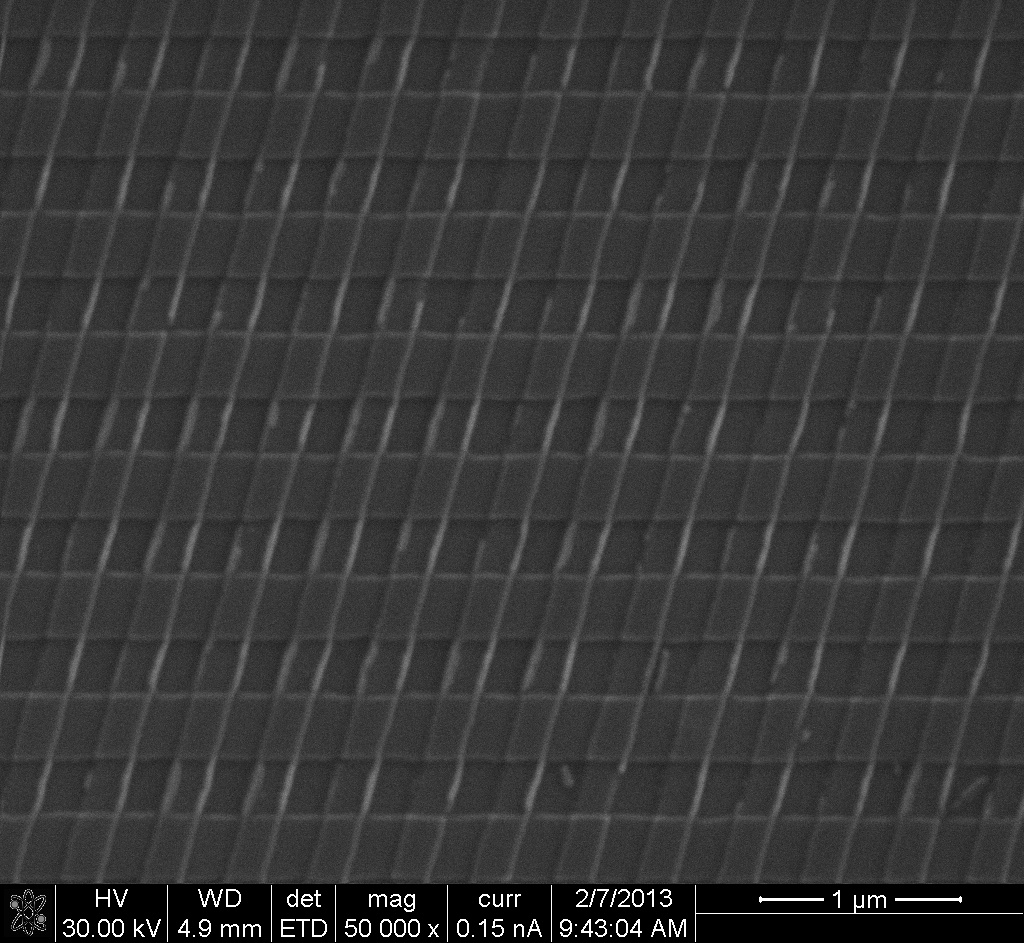
\includegraphics[width=0.4\linewidth]{pic_019}
\caption{SEM of an oblique grating master fabricated in a silicon wafer. \label{fig:obl-sample}}
\end{figure}

The gratings for this chapter were fabricated using electron beam lithography (EBL) and the template stripping method outlined in chapter \ref{c:experimentalmethods}. A scanning electron mircograph of a fabricated oblique grating master in silicon is shown in figure \ref{fig:obl-sample}. The target parameters of this grating were ${\lambda_{gx}= 600 \:\nano\metre}$, ${\lambda_{gv}= 400 \:\nano\metre}, {\Gamma_x=\Gamma_v=0.5,d_1=d_2=40\:\nano\metre}$.

\section{Coupling of Light and SPP Mode Interaction on Oblique Gratings\label{s:ob-coupling}}
A square profile grating such as those fabricated using EBL contain little or no even-Fourier components in their surface profile (see chapter \ref{c:rectangular}). Consequently, the momentum of a plane wave incident on such a grating may be modified with direct scattering events with values of $\pm m\mathbf{k}_g$, where $m$ is odd.  A direct scattering event, where the plane wave is modified by $\pm n\mathbf{k}_g$, where $n$ is even, is not possible on a grating where $\Gamma=0.5$. There does exist, however, the opportunity for the plane wave to be modified by a total value of $\pm n\mathbf{k}_g$ through multiple-scattering processes, summing the contributions from $\pm m\mathbf{k}_g$ scattering events. These multiple scattering events are found in experiment to be so weak that they are rarely experimentally observed. 

These scattering efficiencies also dictate the strength of interaction between counter-propagating SPP modes. Modes that are separated by a direct scattering event will interact strongly. Little, if any, interaction is observed for modes separated by the weaker multiple-scattering process.

\begin{figure}
	\begin{center}
		\subfigure[Model]{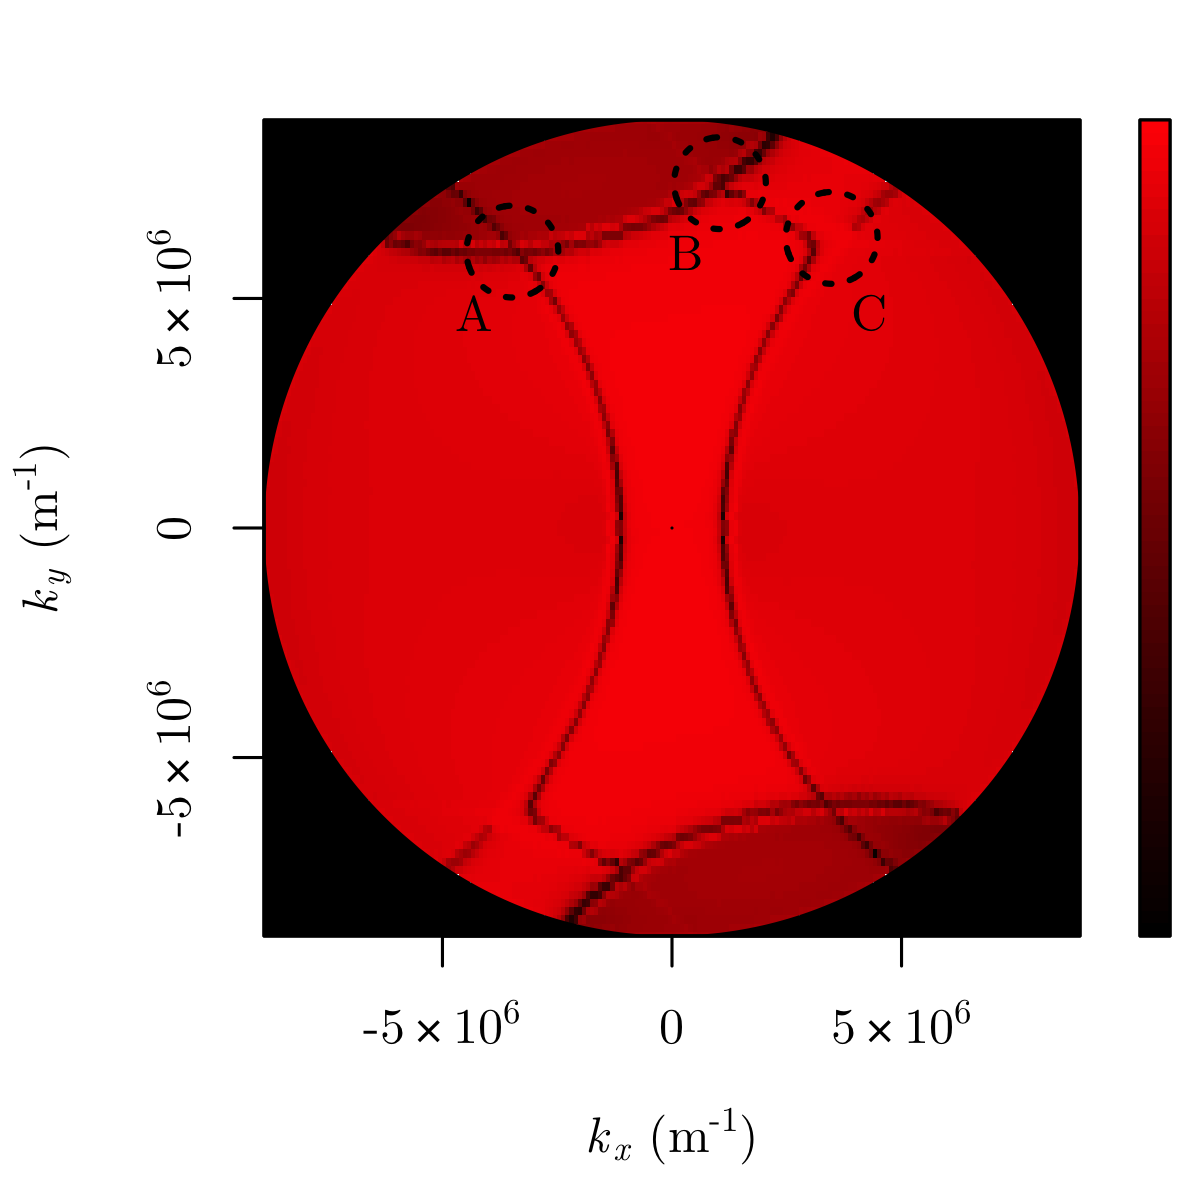
\includegraphics[width=0.49\linewidth]{figure-chandezon-oblique-700nm.png}\label{fig:oblique-chandezon-exp-comparisonA}}
		\subfigure[Experiment]{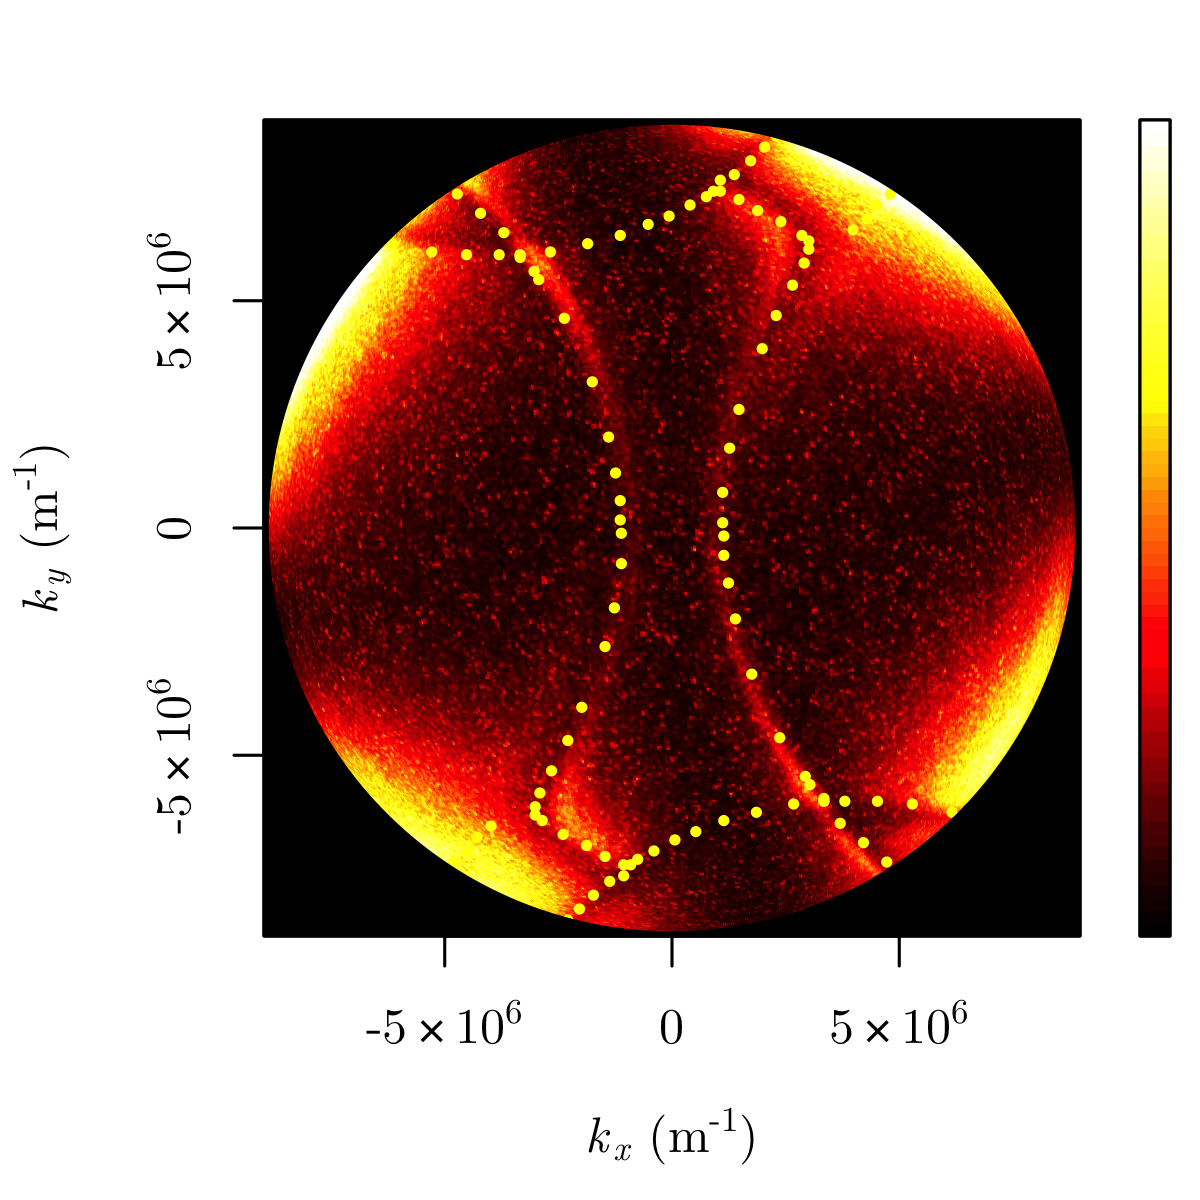
\includegraphics[width=0.49\linewidth]{figure-scatter-oblique-700nm.png}\label{fig:oblique-chandezon-exp-comparisonB}}
	\end{center}
	\caption[The modelled and experimental iso-frequency surface for an oblique bigrating illuminated with TM polarisation at $\lambda_0=700\:\nano\metre$.]{(a) The theoretically modelled iso-frequency surface for an oblique bigrating illuminated with TM polarisation at $\lambda_0=700\:\nano\metre$. Mode intersections labelled A-C are discussed in section \ref{c:experimentalmethods} (b) Experimentally obtained scattergram of the iso-frequency contour imaged through crossed polarisers. The yellow circles overlay indicates the theoretical mode position obtained from (a). Both colour bars range from low reflectivity (black) to high.\label{fig:oblique-chandezon-exp-comparison}}
\end{figure}

Figure \ref{fig:oblique-chandezon-exp-comparison} shows the theoretical and experimentally measured iso-frequency contours for an oblique bigrating at $\lambda_0=700\:\nano\metre$.  Figure \ref{fig:oblique-chandezon-exp-comparisonA} shows the numerical prediction using the Chandezon method, approximating the square groove profiles with the Fourier sums,
\begin{align}
F(x) &= \sum\limits_{n=1}^3  \frac{4A}{n \pi}\cos{\frac{2 n \pi x}{\lambda_{gx}}}\\
F(y) &= \sum\limits_{n=1}^3  \frac{4A}{n \pi}\cos{\frac{2 n \pi v}{\lambda_{gv}}}
\end{align}
Providing a suitable approximation to a lamella bi-grating with a depth of $2A=40\:\nano\metre$, $\lambda_{gx}=600\:\nano\metre$, $\lambda_{gv}=400\:\nano\metre$, $\alpha=75^\circ$ and $\Gamma=0.5$. The dielectric function of silver is taken from literature \cite{Nash1996}, and for the illuminating wavelength of $700\:\nano\metre$ is equal to $\varepsilon=-23.13+0.59i$. The light in the theoretical plot is TM polarised for every azimuthal angle. Only the $n=1,3$ components are included in the calculation, as the even components are considered to be absent for a grating with $\Gamma=0.5$.

The corresponding experimentally obtained iso-frequency surface is shown in figure \ref{fig:oblique-chandezon-exp-comparisonB}. The contour is obtained using imaging scatterometry detailed in chapter \ref{c:experimentalmethods}.  For the illuminating wavelength of $700\:\nano\metre$, the contrast of the entire SPP contour to the background is weak, making the determination of the mode position in $k$-space difficult. To improve the contrast, the polarisers of the scatterometer are crossed, producing a dark background reflectivity against which the polarisation conversion mediated by the SPPs \cite{Bryan-Brown1990} provides greater contrast for the mode positions. The four bright lobes of high reflectivity is polarisation conversion mediated by the ellipsoidal mirror in the apparatus (see chapter \ref{c:experimentalmethods}).  

The modelled values for the mode position (taken from the theoretical plot at the position of reflectivity minima) found in figure \ref{fig:oblique-chandezon-exp-comparisonA} are plotted on the experimental results in figure \ref{fig:oblique-chandezon-exp-comparisonB} as yellow circles, and show good agreement, especially considering the simplicity of the model. This shows that the dominant scattering amplitudes in the observable SPP band structure are only the $n=1,3$ components. 

In the upper half-space of figure \ref{fig:oblique-chandezon-exp-comparisonA}, three SPP contour crossings are labelled A-C\footnote{These mode crossings are equivalent through an inversion symmetry operation to the crossings in the lower half-space}. Crossing point A is the meeting of a $(-1,0)$ and a $(0,1)$ Bragg scattered SPP contour. These two SPP curves are separated in  $k$-space by a minimum of two scattering vectors, and so require a multiple scattering process to interact with each other. With no $2^{nd}$ order harmonics in the grating profile, the interaction is weak and no band-gap is observed. The crossing point B is the intersection of the $(0,1)$ and $(1,1)$ SPPs. This is a process by which the SPPs must scatter a total of $1\mathbf{k}_{gx}$ to interact, and so a small band-gap forms. At point C, the $(1,0)$ and $(1,1)$ SPP cross. These are separated by a single scattering vector $1\mathbf{k}_{gv}$, and so interact, forming a large band-gap.

The coupling efficiencies of plane-polarised light to all these SPP modes is strong as the majority of the contours present are Bragg scattered back into the light circle by a single scattering vector, which is inherent in the grating profile. The exception is the $(1,1)$ SPP, (the contour between points B and C), which is scattered back in to the light circle by a multiple scattering process. It is, however, observed quite strongly between points B and C, though not strongly (and observed as a weak bright band) outside of these points. 

This coupling between points B and C is an example of SPPs `self-coupling', the $(0,1)$ and $(1,0)$ SPPs coupling to the SPP contour close to the crossing points where there is a component of the SPPs that fulfil the required energy and momentum matching conditions for the $(1,1)$ mode. These well coupled $(0,1)$ and $(1,0)$ SPPs resonantly drive the $(1,1)$ SPP, resulting in its observation as a dark band.

\begin{figure}
\begin{center}
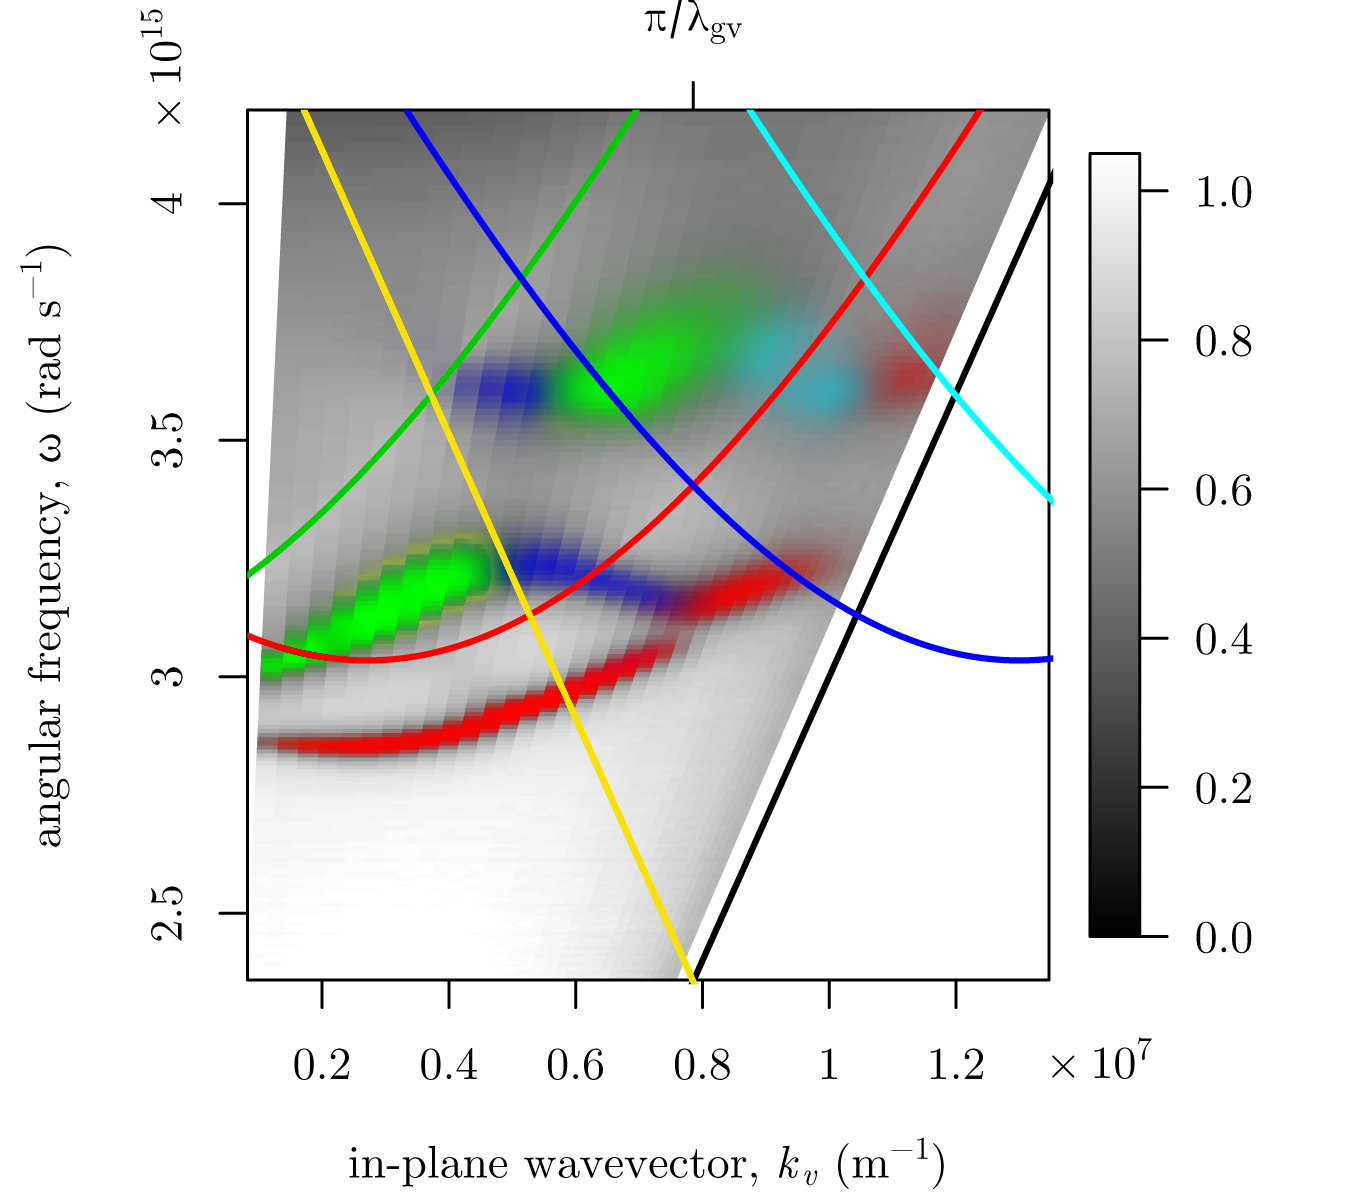
\includegraphics[width=0.6\linewidth]{figure-oblique-RssAtPhi90-colourcoded}
\end{center}
\caption[The dispersion of modes on an oblique grating for $\phi =\alpha =75^\circ$.]{The dispersion of modes on an oblique grating for $\phi =\alpha =75^\circ$, measured using the reflectivity as a function of polar angle and wavelength. The mode positions (grayscale minima) and calculated diffraction edges (lines) have been coloured to correspond to the scattered mode labels given in table \ref{tbl:obliquecouping}.\label{fig:obliquedispcoloured}}
\end{figure}
\begin{table}
\begin{center}
\begin{tabular}{c||c|c|c|c|c|}
$(n,m)$ 	&\color{red}(-1,0)	& \color{green}(1,0) 	& \color{blue}(1,1) 		& \color{cyan}(-1,1) 	& \color{yellow}(0,1) \tabularnewline
\hline
\hline
\color{red}(-1,0)											& 	 	\cellcolor{lightgray}				&  							&  								& 	$\checkmark$			& \tabularnewline
\color{green}(1,0)\color{black} 					& 	 						& \cellcolor{lightgray} 						& $\checkmark$ 			& 								& \tabularnewline
\color{blue}(1,1)\color{black}  					& 		& 		$\checkmark$						& \cellcolor{lightgray}							& 								& $\checkmark$\tabularnewline
\color{cyan}(-1,1)\color{black}  					&$\checkmark$  						& 								&									&\cellcolor{lightgray}							&\tabularnewline
\color{yellow}(0,1)\color{black}  					& 							& 								& 	$\checkmark$	 		 	&							&\cellcolor{lightgray}\tabularnewline
\hline
Light 														& 	 $\checkmark$	& 	 $\checkmark$		& 									& 		 						&$\checkmark^\star$
\end{tabular}
\end{center}
\caption{The expected strong coupling ($\checkmark$) between SPP modes. The colour of the $(n,m)$ mode labels correspond to the highlighted modes in figure \ref{fig:obliquedispcoloured} scattered by ($n\mathbf{k}_{gx},m\mathbf{k}_{gv}$). $\checkmark^\star$ indicates coupling, but only for the orthogonal polarisation (TM) and so is not observed in figure \ref{fig:obliquedispcoloured}. \label{tbl:obliquecouping} }
\end{table}

These interactions can also be observed by mapping the dispersion relation of the SPPs by recording the zero-order reflectivity from the sample as a function of polar angle and wavelength. TE polarised light is incident on the sample and the reflectivity measured for the wavelength range ${400 \:\nano\metre < \lambda_0 < 850 \:\nano\metre}$ and the angle range ${7^\circ<\theta<75^\circ}$ (see chapter \ref{c:experimentalmethods}). These experimental results are shown in figure \ref{fig:obliquedispcoloured} for an azimuthal angle of $\phi=75^\circ$, with the plane of incidence containing $\mathbf{k}_{gv}$. To facilitate the discussion of mode interactions, the dark-bands of low reflectivity which map the SPP dispersion have been colour coded depending upon which dominant scattering event the SPP contour is associated with. The associated diffraction lines have also been coloured accordingly. These scattering interactions between the present modes are summarised in the companion table \ref{tbl:obliquecouping}. 

The band gaps are clearly observed for the interactions between the $(1,0)$ scattered SPP band (green) and the $(1,1)$ scattered SPP band (blue). Another large band-gap is observed for the interaction of the $(-1,1)$ scattered SPP (cyan) and the $(-1,0)$ scattered SPP (red), which again are SPPs separated in $k$-space by a single grating vector of $1\mathbf{k}_{gv}$.

A smaller band-gap is also observed for the $(-1,0)$ and $(1,1)$ SPP crossing (red and blue bands, respectively). This coupling is mediated either by multiple scattering events or a weak direct-scatter due to a small deviation in $\Gamma$ away from the designed value of 0.5, and consequently the frequency gap formed is small in comparison to the other observed band-gaps.

The presence of a dark band associated with the $(1,1)$ scattered SPP is clearly observed in the mapped dispersion and coloured as a blue band of low reflectivity, despite the ($1,1$) scattering event requiring multiple scattering with which to interact with zero-order light. This region of the dispersion is observed for the same reason the iso-frequency contour between points B and C in figure \ref{fig:oblique-chandezon-exp-comparison} is observed, a component of the ($-1,0$) and ($1,0$) SPP fields present on the surface resonantly drive this mode. The SPPs have `self-coupled'. A very small reflectivity minimum (not coloured) lies between the red $(-1,0)$ and the green $(1,0)$ scattered SPP bands. There is also weak self-coupling of these modes to the in-plane $(0,1)$ SPP (its presence cannot be attributed to the incident light field, as the incident light's polarisation state is incorrect for its excitation for this orientation).

\section{Polarisation Conversion}

In this section we discuss how SPPs on an oblique bigrating mediate the rotation of the incident field's polarisation. An example is experimentally demonstrated in figure \ref{fig:oblique-polcov}.

\begin{figure}
\begin{center}
\subfigure[$R_{TE:TE}, \phi=75^\circ$]{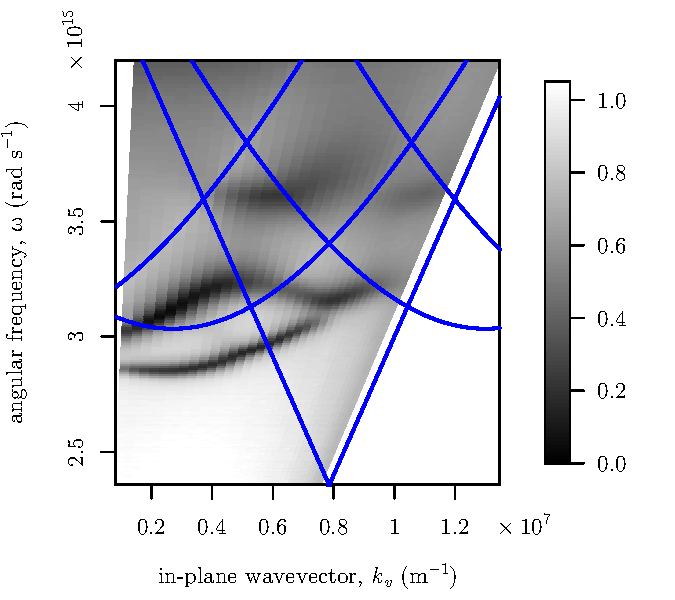
\includegraphics[width=0.49\linewidth]{figure-oblique-RppAtPhi75-Rss}\label{fig:oblique-polcovA}}
\subfigure[$R_{TE:TM}, \phi=75^\circ$]{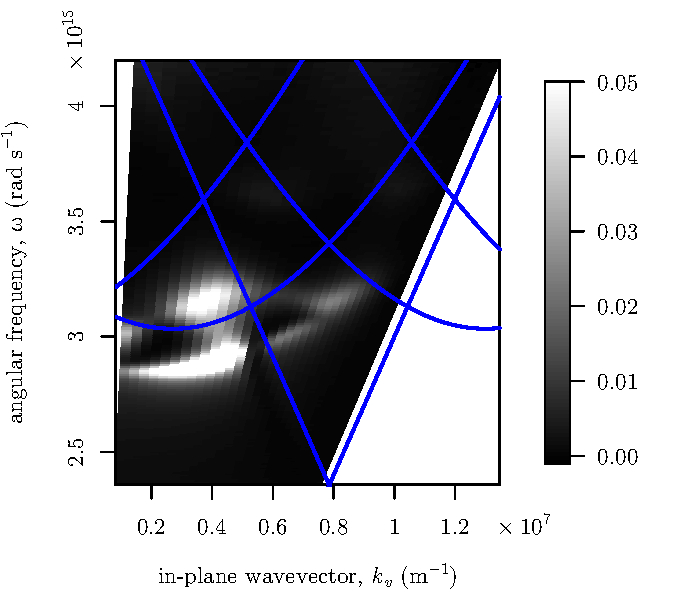
\includegraphics[width=0.49\linewidth]{figure-oblique-RppAtPhi75-Rsp}\label{fig:oblique-polcovB}}
\end{center}
\caption[Polarisation conservation and conversion mediated by out-of-plane scattered SPPs on an oblique grating.]{(a) Polarisation conservation and (b) conversion mediated by out-of-plane scattered SPPs on an oblique grating.\label{fig:oblique-polcov}}
\end{figure}

This figure shows the reflectivity of an oblique grating as a function of $(\omega,k_v)$, mapping the SPP dispersion by the characteristic minima in reflected intensity.  For subfigure \ref{fig:oblique-polcovA}, the incident polarisation is set to be TE polarised, and the detector's polariser is also set to TE. The corresponding polarisation conversion signal is recorded by rotating the detector's polariser by $90^\circ$ to TM, and is shown in figure \ref{fig:oblique-polcovB}. The bright bands of polarisation converted signal lie along the same SPP contours, showing that it is the surface waves which mediate this polarisation conversion.

The polarisation converted signal is normalised to the reference spectrum with both polarisers set to TE polarised, and with this definition, only a maximum of $\approx 5\%$ of the light coupled into the SPPs is re-radiated in to the orthogonal polarisation state. Additionally, the SPP modes in the plane (which travel collinear to the wavevector $\mathbf{k}_{gv}$), do not participate in this polarisation conversion as the SPPs are travelling along a mirror-plane of the grating associated with the $\mathbf{k}_{gv}$ direction (although there are no mirror planes associated with the overall bigrating structure). This is an important point: SPP mediated polarisation conversion occurs only when the SPPs are travelling along the surface in a direction out of the plane of incidence and along a direction of broken mirror symmetry. An oblique bigrating always provides out-of-plane scattering mechanisms and so polarisation conversion will always be observed for out-of-plane scattered SPPs. If, however, the plane of incidence contains a grating vector, conservation of momentum dictates that the SPP associated with this grating vector will travel along  in the plane of incidence and polarisation conversion does not occur, even though the SPP is traversing a surface of broken symmetry.

\section{SPPs at the BZ Boundary of Oblique Bigratings\label{s:ob-BZ}}
The formation of photonic band-gaps on an oblique bigrating is of interest, as in this section we present results that show that on a surface with such broken symmetry the locations in $k$-space of SPP standing waves do not necessarily occur at the BZ boundary. This concept is known for the band-gaps that occur for electron propagation in semiconductor crystals \cite{Iva}, but has not previously been demonstrated for SPPs on gratings. To show this clearly, we must identify how photonic band-gaps are illustrated in the iso-frequency contours recorded with imaging scatterometry.
The iso-frequency image obtained using scatterometry maps $k$-space at a single frequency, with SPP bands seen as an anomaly in the reflected light. 
The group velocity of a general propagating wave is defined as,
\begin{equation}
\mathbf{v}_g = \nabla_k\: \omega(\mathbf{k})
\end{equation}
where $\mathbf{v}_g$ is the group velocity, $\omega(\mathbf{k})$ is the angular frequency of the wave as a function of wavevector, $\mathbf{k}$, and $\nabla_k$ is the gradient operator with respect to $k$. For a small change in frequency $d\omega$, the corresponding small movement in $k$-space, $d\mathbf{k}$, is related to this group velocity simply by,
\begin{equation}
d\omega = \nabla_k\: \omega(\mathbf{k}) \cdot d\mathbf{k}
\end{equation}
For an iso-frequency contour, there must be no change in frequency along the contour ($d\omega=0$). Setting $d\omega=0$ restricts the values of $d\mathbf{k}$ to those values that move along a contour of equal frequency. It is then apparent that in the resultant expression,
\begin{equation}
\mathbf{v}_g \cdot d\mathbf{k} = 0
\end{equation}
that $\mathbf{v}_g$ lies perpendicular to $d\mathbf{k}$.
This is true for any general contour of constant frequency. If the group velocity in one direction falls to zero at a boundary, such as at the BZ boundary,  the iso-frequency SPP contour will intersect that boundary perpendicularly.

Plasmonic band-gaps on surface relief gratings are covered in chapter \ref{c:backgroundtheory}. To briefly recap, when a SPP meets an equivalent, counter-propagating SPP a standing wave forms. There are generally two possible arrangements of the electric field  for a SPP standing wave on a grating, which will generally differ in energy. This leads to an upper and lower energy band, with an energy range between where SPP propagation is forbidden.
The energy gap size is dependent on the energy of the two possible field distributions, and so is linked intimately to the surface geometry. The surface profile also provides the scattering mechanism by which SPPs Bragg scatter to meet counter-propagating SPPs and form these standing waves. The strength of this scattering, and so the amplitude of the Bragg scattered SPP, was discussed earlier in chapter \ref{c:rectangular} and affects the magnitude in energy of the band-gap.

\begin{figure}
\begin{center}
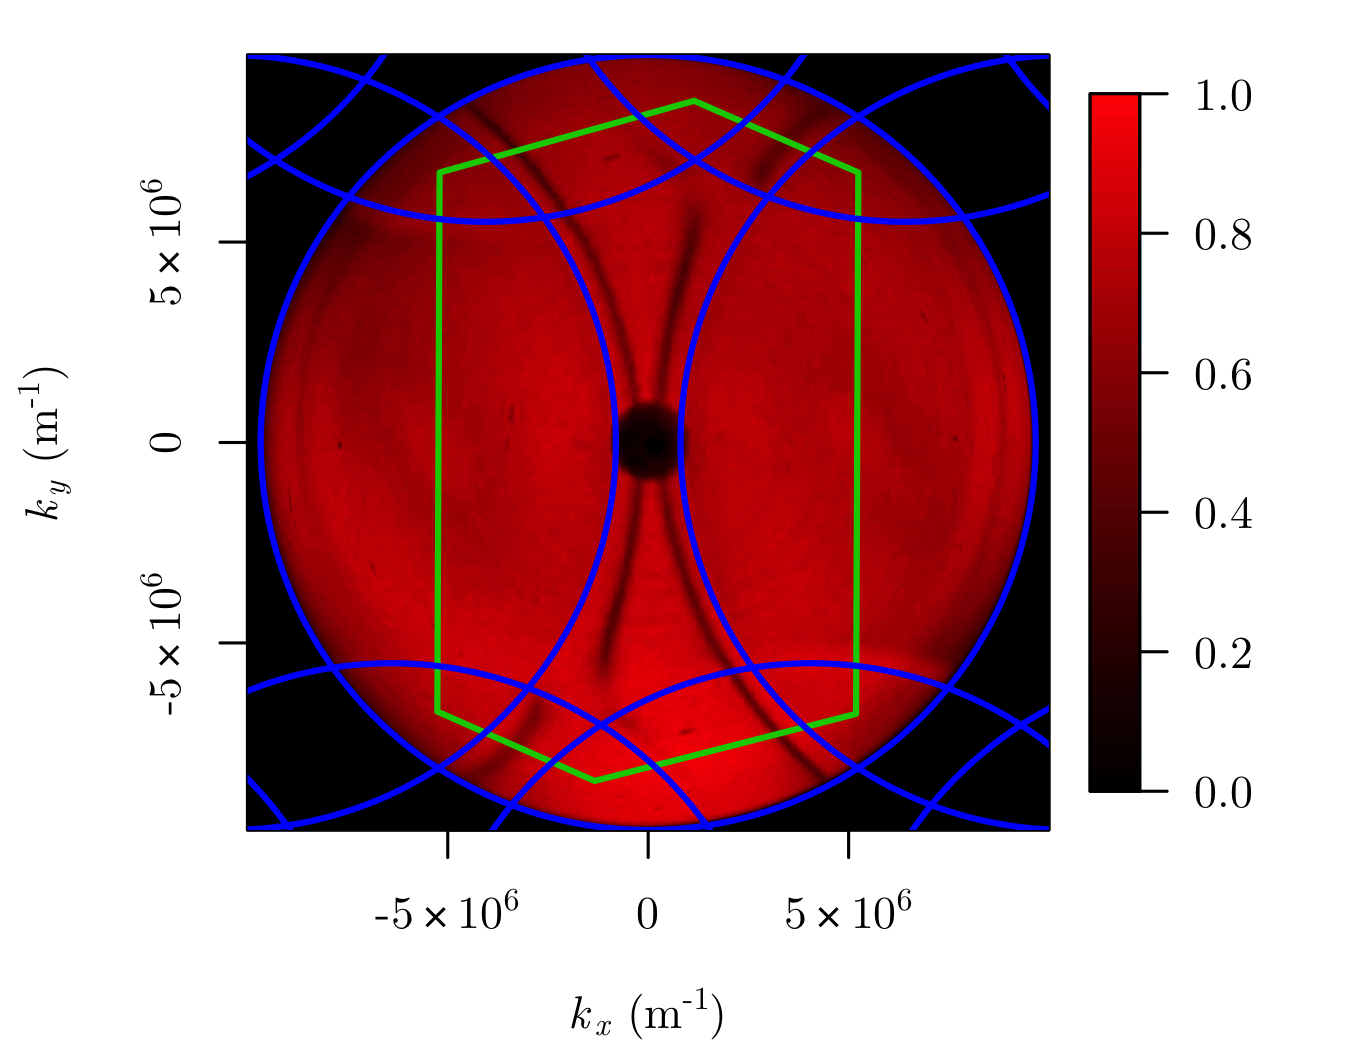
\includegraphics[width=0.7\linewidth]{figure-650nm-scattergram-withBZ}
\end{center}
\caption[An experimentally obtained iso-frequency contour map of SPPs on an oblique bigrating with illuminated with incident light of wavelength $\lambda_0=650\:\nano\metre$.]{An experimentally obtained iso-frequency contour map of SPPs on an oblique bigrating with illuminated with incident light of wavelength $\lambda_0=650\:\nano\metre$. SPP positions are mapped as regions of low reflectivity. The blue circles indicate diffracted light circles, and the green region is the typical BZ boundary drawn using the Wigner-Seitz method.\label{fig:ob-650scatterALL}}
\end{figure}

\begin{figure}
\begin{center}
\subfigure[]{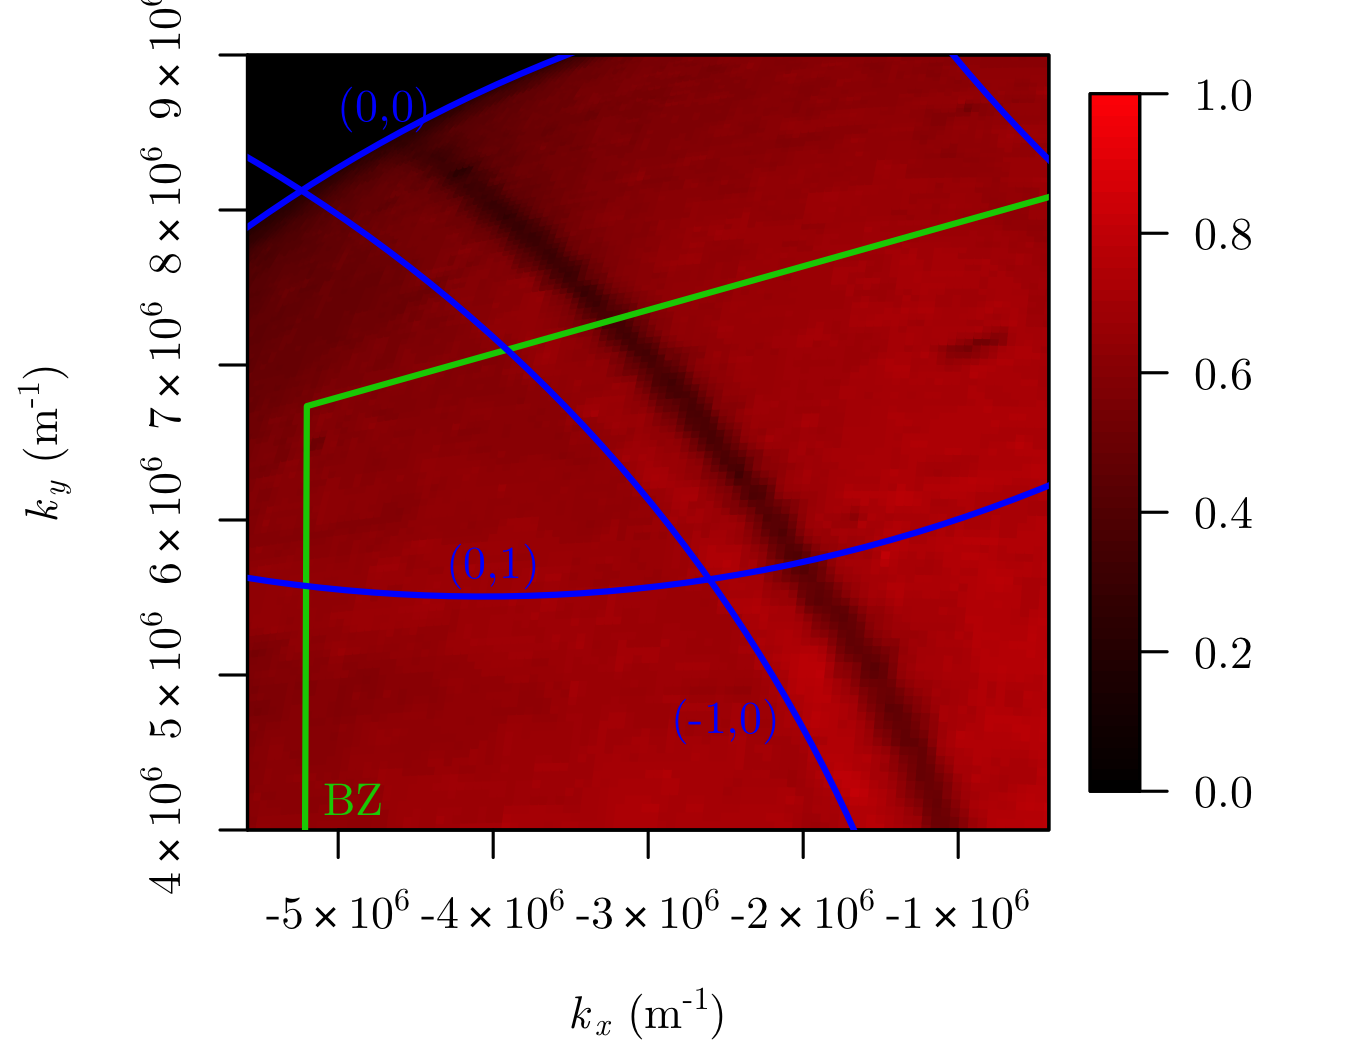
\includegraphics[width=0.48\linewidth]{figure-650nm-scattergram-withBZ-zoom1}\label{fig:obl-scattZoomA}}
\subfigure[]{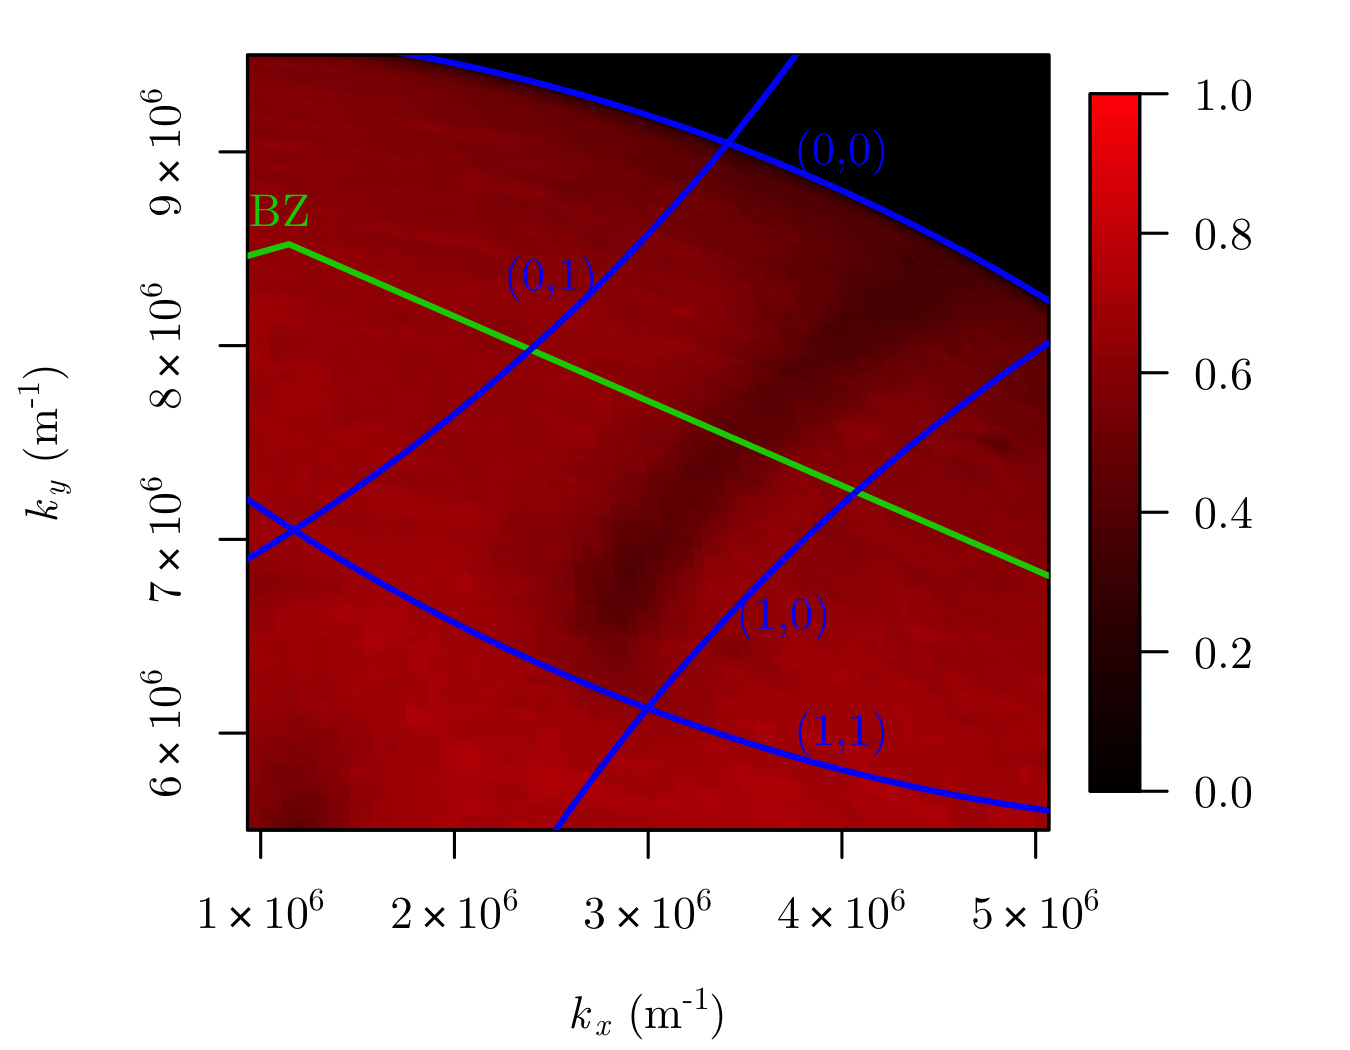
\includegraphics[width=0.48\linewidth]{figure-650nm-scattergram-withBZ-zoom2}\label{fig:obl-scattZoomB}}
\end{center}
\caption[Regions of interest from figure \ref{fig:ob-650scatterALL}.]{Regions of interest from figure \ref{fig:ob-650scatterALL}. (a) The $(-1,0)$ scattered SPP contour at the BZ boundary and (b) the $(+1,0)$ scattered SPP contour at the BZ boundary.\label{fig:obl-scattZoom}}
\end{figure}

Figure \ref{fig:ob-650scatterALL} shows the mapped iso-frequency contours of SPPs for the oblique grating at a wavelength of $\lambda_0=650\:\nano\metre$. The position of the SPP contours are found to present as bands of low reflectivity, with the polariser of the experiment chosen in this case to best couple light to the $(\pm 1,0)$ modes. Also annotated on the figure are the diffracted light circles (blue lines) and the BZ boundary formed using the Wigner-Seitz method \cite{kittel1996introduction} (green line).

It is observed that the SPP contour passes through the BZ boundary  seemingly unperturbed. Figure \ref{fig:obl-scattZoom} shows the two regions in which this occurs in greater detail. In figure \ref{fig:obl-scattZoomA} the SPP contour following the $(-1,0)$ diffracted light circle is shown to pass through the BZ at an angle which is not perpendicular to the boundary. This means that at the boundary, the SPP's group velocity in the $(0,1)$ direction is not zero, and no standing-wave states in this direction have formed. The $(0,1)$ scattered SPP is not observed in this figure as the polarisation of the illuminating light has been chosen to only couple strongly to the $(1,0)$ SPP. Additionally the $(-1,0)$ and (uncoupled) $(0,1)$ SPPs are not seen to interact, separated as they are by a weak multiple scattering process. 

The same behaviour is observed in the second region in figure \ref{fig:obl-scattZoomB}. Here, a band-gap has formed inside the BZ\footnote{Recall that the SPP eigenmodes are unaffected by the coupling of the light, and so although some branches of the SPP contours are uncoupled to light in this scattergram, the band-gap still exists.}, but the group velocity at the BZ boundary is still finite. This highlights the fact that the mode crossing positions on an oblique grating do not coincide with BZ boundary constructed using the Wigner-Seitz method. 

A Brillioun Zone boundary in reciprocal space outlines a unit cell in the reciprocal lattice and contains on the boundary points of high-symmetry. One way to determine a boundary that contains the maximum amount of high-symmetry points is to connect the perpendicular bisectors of the vectors connecting the nearest neighbours to one lattice point, a method known as the Wigner-Seitz method. The area mapped out by this method, for the highly-symmetric cases of square, rectangular or hexagonal lattices, is exactly equivalent to the area we call the Brillioun Zone, and no other choice of unit cell contains as many points of high-symmetry in the boundary.

\begin{figure}
\centering %LaTeX with PSTricks extensions
%%Creator: inkscape 0.48.2
%%Please note this file requires PSTricks extensions
\psset{xunit=.5pt,yunit=.5pt,runit=.5pt}
\begin{pspicture}(359.92419434,324.88348389)
{
\newrgbcolor{curcolor}{0 0 0}
\pscustom[linewidth=1.84079344,linecolor=curcolor]
{
\newpath
\moveto(179.95596336,162.43775739)
\lineto(179.95596336,162.43775739)
}
}
{
\newrgbcolor{curcolor}{0 0 0}
\pscustom[linestyle=none,fillstyle=solid,fillcolor=curcolor]
{
\newpath
\moveto(13.25861844,6.62318327)
\curveto(13.25861844,-2.20771645)(-0.00000309,-2.20771645)(-0.00000309,6.62318327)
\curveto(-0.00000309,15.46144616)(13.25861844,15.46144616)(13.25861844,6.62318327)
}
}
{
\newrgbcolor{curcolor}{0 0 0}
\pscustom[linestyle=none,fillstyle=solid,fillcolor=curcolor]
{
\newpath
\moveto(37.29447196,318.25478589)
\curveto(37.29447196,309.42388618)(24.04566799,309.42388618)(24.04566799,318.25478589)
\curveto(24.04566799,327.09304878)(37.29447196,327.09304878)(37.29447196,318.25478589)
}
}
{
\newrgbcolor{curcolor}{0 0 0}
\pscustom[linestyle=none,fillstyle=solid,fillcolor=curcolor]
{
\newpath
\moveto(335.87853069,6.62318327)
\curveto(335.87853069,-2.20771645)(322.62727233,-2.20771645)(322.62727233,6.62318327)
\curveto(322.62727233,15.46144616)(335.87853069,15.46144616)(335.87853069,6.62318327)
}
}
{
\newrgbcolor{curcolor}{0 0 0}
\pscustom[linestyle=none,fillstyle=solid,fillcolor=curcolor]
{
\newpath
\moveto(294.12442675,162.43775739)
\curveto(294.12442675,153.60931206)(280.87562278,153.60931206)(280.87562278,162.43775739)
\curveto(280.87562278,171.27847467)(294.12442675,171.27847467)(294.12442675,162.43775739)
}
}
{
\newrgbcolor{curcolor}{0 0 0}
\pscustom[linestyle=none,fillstyle=solid,fillcolor=curcolor]
{
\newpath
\moveto(359.92420177,318.25478589)
\curveto(359.92420177,309.42388618)(346.66312584,309.42388618)(346.66312584,318.25478589)
\curveto(346.66312584,327.09304878)(359.92420177,327.09304878)(359.92420177,318.25478589)
}
}
{
\newrgbcolor{curcolor}{0.88235295 0 0}
\pscustom[linewidth=1.963513,linecolor=curcolor,strokeopacity=0.29411766,linestyle=dashed,dash=2 1]
{
\newpath
\moveto(114.1684603,6.62595182)
\lineto(245.7508296,318.25754659)
\lineto(245.7508296,318.25754659)
}
}
{
\newrgbcolor{curcolor}{0.88235295 0 0}
\pscustom[linewidth=1.963513,linecolor=curcolor,strokeopacity=0.29411766,linestyle=dashed,dash=2 1]
{
\newpath
\moveto(138.20922259,318.25754659)
\lineto(221.71006731,6.62595182)
}
}
{
\newrgbcolor{curcolor}{0.88235295 0 0}
\pscustom[linewidth=1.963513,linecolor=curcolor,strokeopacity=0.29411766,linestyle=dashed,dash=2 2]
{
\newpath
\moveto(72.41926513,162.44235201)
\lineto(287.50002476,162.44235201)
}
}
{
\newrgbcolor{curcolor}{0.88235295 0 0}
\pscustom[linewidth=1.963513,linecolor=curcolor]
{
\newpath
\moveto(125.77635645,93.30028516)
\lineto(125.77635645,232.17918658)
\lineto(191.82653828,249.58429596)
\lineto(233.41558933,232.19628878)
\lineto(233.41558933,93.17454178)
\lineto(167.57061424,75.35403159)
\closepath
}
}
{
\newrgbcolor{curcolor}{0 0 0.88235295}
\pscustom[linewidth=1.963513,linecolor=curcolor]
{
\newpath
\moveto(92.81013165,84.42063141)
\lineto(158.80144737,240.88175109)
\lineto(265.71575124,240.84208812)
\lineto(201.07079676,84.42053324)
\closepath
}
}
{
\newrgbcolor{curcolor}{0 1 0}
\pscustom[linestyle=none,fillstyle=solid,fillcolor=curcolor]
{
\newpath
\moveto(104.42550261,192.58960702)
\lineto(106.54241506,192.58960702)
\lineto(106.54241506,179.70405296)
\lineto(104.42550261,179.70405296)
\lineto(104.42550261,192.58960702)
\moveto(104.42550261,197.60576914)
\lineto(106.54241506,197.60576914)
\lineto(106.54241506,194.92511369)
\lineto(104.42550261,194.92511369)
\lineto(104.42550261,197.60576914)
}
}
{
\newrgbcolor{curcolor}{0 1 0}
\pscustom[linestyle=none,fillstyle=solid,fillcolor=curcolor]
{
\newpath
\moveto(110.63935771,176.26293744)
\lineto(113.10720617,176.26293744)
\lineto(113.10720617,184.7807538)
\lineto(110.42248618,184.24231413)
\lineto(110.42248618,185.61832661)
\lineto(113.09224951,186.15676627)
\lineto(114.6028719,186.15676627)
\lineto(114.6028719,176.26293744)
\lineto(117.07072037,176.26293744)
\lineto(117.07072037,174.99162157)
\lineto(110.63935771,174.99162157)
\lineto(110.63935771,176.26293744)
}
}
{
\newrgbcolor{curcolor}{0 1 0}
\pscustom[linestyle=none,fillstyle=solid,fillcolor=curcolor]
{
\newpath
\moveto(248.92344313,144.88453428)
\lineto(251.04035558,144.88453428)
\lineto(251.04035558,131.99898021)
\lineto(248.92344313,131.99898021)
\lineto(248.92344313,144.88453428)
\moveto(248.92344313,149.90069639)
\lineto(251.04035558,149.90069639)
\lineto(251.04035558,147.22004095)
\lineto(248.92344313,147.22004095)
\lineto(248.92344313,149.90069639)
}
}
{
\newrgbcolor{curcolor}{0 1 0}
\pscustom[linestyle=none,fillstyle=solid,fillcolor=curcolor]
{
\newpath
\moveto(257.4601227,149.17588398)
\lineto(257.4601227,142.79063174)
\lineto(255.50427967,142.79063174)
\lineto(255.50427967,149.17588398)
\lineto(257.4601227,149.17588398)
}
}
{
\newrgbcolor{curcolor}{0 1 0}
\pscustom[linestyle=none,fillstyle=solid,fillcolor=curcolor]
{
\newpath
\moveto(261.6260951,128.5578647)
\lineto(264.09394356,128.5578647)
\lineto(264.09394356,137.07568106)
\lineto(261.40922357,136.53724139)
\lineto(261.40922357,137.91325387)
\lineto(264.0789869,138.45169353)
\lineto(265.58960929,138.45169353)
\lineto(265.58960929,128.5578647)
\lineto(268.05745776,128.5578647)
\lineto(268.05745776,127.28654883)
\lineto(261.6260951,127.28654883)
\lineto(261.6260951,128.5578647)
}
}
{
\newrgbcolor{curcolor}{0 1 0}
\pscustom[linestyle=none,fillstyle=solid,fillcolor=curcolor]
{
\newpath
\moveto(136.69903978,266.09694715)
\lineto(138.81595223,266.09694715)
\lineto(138.81595223,253.21139309)
\lineto(136.69903978,253.21139309)
\lineto(136.69903978,266.09694715)
\moveto(136.69903978,271.11310927)
\lineto(138.81595223,271.11310927)
\lineto(138.81595223,268.43245382)
\lineto(136.69903978,268.43245382)
\lineto(136.69903978,271.11310927)
}
}
{
\newrgbcolor{curcolor}{0 1 0}
\pscustom[linestyle=none,fillstyle=solid,fillcolor=curcolor]
{
\newpath
\moveto(143.95238256,249.77027757)
\lineto(149.22460428,249.77027757)
\lineto(149.22460428,248.4989617)
\lineto(142.1351487,248.4989617)
\lineto(142.1351487,249.77027757)
\curveto(142.70848553,250.36355645)(143.48872371,251.15875127)(144.47586557,252.15586442)
\curveto(145.46798605,253.1579558)(146.09117949,253.8035842)(146.34544774,254.09275155)
\curveto(146.82904051,254.63617062)(147.16556496,255.09484099)(147.35502211,255.46876402)
\curveto(147.54945212,255.84765866)(147.64667029,256.21908194)(147.64667693,256.58303499)
\curveto(147.64667029,257.17630706)(147.4372773,257.65990516)(147.01849732,258.03383075)
\curveto(146.60469087,258.40773728)(146.06375898,258.59469531)(145.3957,258.5947054)
\curveto(144.92206861,258.59469531)(144.42102109,258.51243378)(143.89255593,258.34792056)
\curveto(143.36907057,258.18338764)(142.80819648,257.93411027)(142.20993198,257.60008769)
\lineto(142.20993198,259.12566674)
\curveto(142.81816758,259.36994794)(143.38651999,259.5544132)(143.91499092,259.67906306)
\curveto(144.44345605,259.80369057)(144.92705415,259.86600991)(145.36578668,259.86602128)
\curveto(146.52242934,259.86600991)(147.44475562,259.57684816)(148.13276829,258.99853515)
\curveto(148.82076672,258.42020115)(149.1647695,257.64744129)(149.16477765,256.68025327)
\curveto(149.1647695,256.22157472)(149.07752242,255.78533931)(148.90303614,255.37154575)
\curveto(148.73351964,254.96272398)(148.42192292,254.47912588)(147.96824506,253.92074999)
\curveto(147.84359942,253.77616369)(147.4472484,253.3573777)(146.7791908,252.66439077)
\curveto(146.11112168,251.97638105)(145.16885321,251.01167762)(143.95238256,249.77027757)
}
}
{
\newrgbcolor{curcolor}{0 1 0}
\pscustom[linestyle=none,fillstyle=solid,fillcolor=curcolor]
{
\newpath
\moveto(217.12008128,72.28992089)
\lineto(219.23699373,72.28992089)
\lineto(219.23699373,59.40436683)
\lineto(217.12008128,59.40436683)
\lineto(217.12008128,72.28992089)
\moveto(217.12008128,77.30608301)
\lineto(219.23699373,77.30608301)
\lineto(219.23699373,74.62542756)
\lineto(217.12008128,74.62542756)
\lineto(217.12008128,77.30608301)
}
}
{
\newrgbcolor{curcolor}{0 1 0}
\pscustom[linestyle=none,fillstyle=solid,fillcolor=curcolor]
{
\newpath
\moveto(225.65676084,76.58127059)
\lineto(225.65676084,70.19601836)
\lineto(223.70091782,70.19601836)
\lineto(223.70091782,76.58127059)
\lineto(225.65676084,76.58127059)
}
}
{
\newrgbcolor{curcolor}{0 1 0}
\pscustom[linestyle=none,fillstyle=solid,fillcolor=curcolor]
{
\newpath
\moveto(230.86222093,55.96325132)
\lineto(236.13444264,55.96325132)
\lineto(236.13444264,54.69193544)
\lineto(229.04498706,54.69193544)
\lineto(229.04498706,55.96325132)
\curveto(229.6183239,56.55653019)(230.39856208,57.35172501)(231.38570394,58.34883816)
\curveto(232.37782442,59.35092954)(233.00101785,59.99655794)(233.25528611,60.28572529)
\curveto(233.73887888,60.82914437)(234.07540333,61.28781473)(234.26486048,61.66173776)
\curveto(234.45929049,62.0406324)(234.55650866,62.41205569)(234.55651529,62.77600873)
\curveto(234.55650866,63.3692808)(234.34711567,63.8528789)(233.92833569,64.2268045)
\curveto(233.51452924,64.60071102)(232.97359734,64.78766905)(232.30553836,64.78767915)
\curveto(231.83190697,64.78766905)(231.33085945,64.70540752)(230.8023943,64.5408943)
\curveto(230.27890894,64.37636139)(229.71803485,64.12708401)(229.11977035,63.79306143)
\lineto(229.11977035,65.31864048)
\curveto(229.72800594,65.56292168)(230.29635835,65.74738694)(230.82482929,65.8720368)
\curveto(231.35329442,65.99666431)(231.83689252,66.05898365)(232.27562505,66.05899502)
\curveto(233.43226771,66.05898365)(234.35459399,65.7698219)(235.04260666,65.1915089)
\curveto(235.73060509,64.61317489)(236.07460786,63.84041503)(236.07461601,62.87322701)
\curveto(236.07460786,62.41454846)(235.98736078,61.97831306)(235.81287451,61.56451949)
\curveto(235.64335801,61.15569773)(235.33176129,60.67209962)(234.87808343,60.11372373)
\curveto(234.75343779,59.96913743)(234.35708676,59.55035144)(233.68902917,58.85736451)
\curveto(233.02096004,58.1693548)(232.07869157,57.20465136)(230.86222093,55.96325132)
}
}
{
\newrgbcolor{curcolor}{0 1 0}
\pscustom[linestyle=none,fillstyle=solid,fillcolor=curcolor]
{
\newpath
\moveto(231.19843593,265.5612475)
\lineto(233.31534838,265.5612475)
\lineto(233.31534838,252.67569343)
\lineto(231.19843593,252.67569343)
\lineto(231.19843593,265.5612475)
\moveto(231.19843593,270.57740961)
\lineto(233.31534838,270.57740961)
\lineto(233.31534838,267.89675417)
\lineto(231.19843593,267.89675417)
\lineto(231.19843593,270.57740961)
}
}
{
\newrgbcolor{curcolor}{0 1 0}
\pscustom[linestyle=none,fillstyle=solid,fillcolor=curcolor]
{
\newpath
\moveto(241.72728667,253.98331663)
\curveto(242.45018484,253.82875864)(243.01355171,253.50719082)(243.41738895,253.01861223)
\curveto(243.82619594,252.53002352)(244.03060339,251.92677228)(244.03061191,251.20885669)
\curveto(244.03060339,250.10704746)(243.65170178,249.25451884)(242.89390595,248.65126828)
\curveto(242.13609535,248.04801635)(241.0592171,247.74639073)(239.66326796,247.74639052)
\curveto(239.19462235,247.74639073)(238.71102425,247.79375343)(238.2124722,247.88847876)
\curveto(237.7189003,247.97821869)(237.20788169,248.11532124)(236.67941482,248.29978684)
\lineto(236.67941482,249.75806093)
\curveto(237.09819964,249.51376731)(237.55687001,249.32930205)(238.0554273,249.20466461)
\curveto(238.5539795,249.08002468)(239.07496921,249.01770533)(239.61839799,249.01770639)
\curveto(240.5656479,249.01770533)(241.28605951,249.20466336)(241.77963498,249.57858104)
\curveto(242.27818345,249.95249548)(242.52746083,250.49592016)(242.52746784,251.20885669)
\curveto(242.52746083,251.86694571)(242.29563287,252.3804571)(241.83198328,252.7493924)
\curveto(241.37330659,253.12330367)(240.73266374,253.3102617)(239.91005281,253.31026705)
\lineto(238.60882362,253.31026705)
\lineto(238.60882362,254.55166961)
\lineto(239.96987944,254.55166961)
\curveto(240.71272155,254.55166302)(241.28107396,254.69873667)(241.67493837,254.992891)
\curveto(242.06879046,255.29201682)(242.26571959,255.7207739)(242.26572634,256.27916353)
\curveto(242.26571959,256.85249317)(242.06131214,257.29122135)(241.65250339,257.59534937)
\curveto(241.2486679,257.90444369)(240.66785162,258.05899566)(239.91005281,258.05900575)
\curveto(239.49624797,258.05899566)(239.05253425,258.01412573)(238.5789103,257.92439584)
\curveto(238.10528023,257.83464602)(237.58429052,257.69505069)(237.01593961,257.50560943)
\lineto(237.01593961,258.85170859)
\curveto(237.58927607,259.01123522)(238.12522242,259.13088836)(238.62378028,259.21066837)
\curveto(239.12731746,259.29042588)(239.60094447,259.33031026)(240.04466272,259.33032163)
\curveto(241.19133411,259.33031026)(242.09870375,259.06856902)(242.76677436,258.54509712)
\curveto(243.43483047,258.0265896)(243.76886215,257.32362741)(243.7688704,256.43620843)
\curveto(243.76886215,255.81799207)(243.59187521,255.29450959)(243.23790907,254.86575941)
\curveto(242.88392747,254.44198097)(242.38038718,254.14783367)(241.72728667,253.98331663)
}
}
{
\newrgbcolor{curcolor}{0 1 0}
\pscustom[linestyle=none,fillstyle=solid,fillcolor=curcolor]
{
\newpath
\moveto(111.56055459,75.05542541)
\lineto(113.67746705,75.05542541)
\lineto(113.67746705,62.16987134)
\lineto(111.56055459,62.16987134)
\lineto(111.56055459,75.05542541)
\moveto(111.56055459,80.07158752)
\lineto(113.67746705,80.07158752)
\lineto(113.67746705,77.39093208)
\lineto(111.56055459,77.39093208)
\lineto(111.56055459,80.07158752)
}
}
{
\newrgbcolor{curcolor}{0 1 0}
\pscustom[linestyle=none,fillstyle=solid,fillcolor=curcolor]
{
\newpath
\moveto(120.09723416,79.34677511)
\lineto(120.09723416,72.96152287)
\lineto(118.14139113,72.96152287)
\lineto(118.14139113,79.34677511)
\lineto(120.09723416,79.34677511)
}
}
{
\newrgbcolor{curcolor}{0 1 0}
\pscustom[linestyle=none,fillstyle=solid,fillcolor=curcolor]
{
\newpath
\moveto(128.5782022,63.47749454)
\curveto(129.30110037,63.32293655)(129.86446723,63.00136873)(130.26830448,62.51279014)
\curveto(130.67711147,62.02420143)(130.88151892,61.42095019)(130.88152743,60.7030346)
\curveto(130.88151892,59.60122537)(130.50261731,58.74869675)(129.74482148,58.14544619)
\curveto(128.98701088,57.54219426)(127.91013263,57.24056864)(126.51418349,57.24056843)
\curveto(126.04553788,57.24056864)(125.56193978,57.28793134)(125.06338773,57.38265667)
\curveto(124.56981583,57.4723966)(124.05879722,57.60949915)(123.53033035,57.79396475)
\lineto(123.53033035,59.25223884)
\curveto(123.94911517,59.00794522)(124.40778554,58.82347996)(124.90634283,58.69884252)
\curveto(125.40489503,58.57420259)(125.92588474,58.51188325)(126.46931352,58.5118843)
\curveto(127.41656343,58.51188325)(128.13697504,58.69884128)(128.6305505,59.07275895)
\curveto(129.12909898,59.44667339)(129.37837636,59.99009807)(129.37838337,60.7030346)
\curveto(129.37837636,61.36112362)(129.1465484,61.87463501)(128.68289881,62.24357031)
\curveto(128.22422212,62.61748158)(127.58357927,62.80443961)(126.76096834,62.80444496)
\lineto(125.45973915,62.80444496)
\lineto(125.45973915,64.04584752)
\lineto(126.82079497,64.04584752)
\curveto(127.56363708,64.04584093)(128.13198949,64.19291458)(128.5258539,64.48706891)
\curveto(128.91970599,64.78619473)(129.11663512,65.21495181)(129.11664187,65.77334144)
\curveto(129.11663512,66.34667108)(128.91222767,66.78539926)(128.50341892,67.08952729)
\curveto(128.09958343,67.3986216)(127.51876715,67.55317357)(126.76096834,67.55318366)
\curveto(126.3471635,67.55317357)(125.90344978,67.50830364)(125.42982583,67.41857375)
\curveto(124.95619576,67.32882393)(124.43520605,67.1892286)(123.86685514,66.99978734)
\lineto(123.86685514,68.3458865)
\curveto(124.4401916,68.50541313)(124.97613795,68.62506627)(125.47469581,68.70484628)
\curveto(125.97823299,68.78460379)(126.45186,68.82448817)(126.89557825,68.82449954)
\curveto(128.04224964,68.82448817)(128.94961928,68.56274693)(129.61768989,68.03927503)
\curveto(130.285746,67.52076751)(130.61977768,66.81780532)(130.61978593,65.93038634)
\curveto(130.61977768,65.31216998)(130.44279074,64.7886875)(130.0888246,64.35993732)
\curveto(129.734843,63.93615888)(129.23130271,63.64201158)(128.5782022,63.47749454)
}
}
{
\newrgbcolor{curcolor}{0 1 0}
\pscustom[linestyle=none,fillstyle=solid,fillcolor=curcolor]
{
\newpath
\moveto(129.14847849,162.65118356)
\curveto(129.14847849,160.80506763)(127.65190583,159.30849496)(125.80578989,159.30849496)
\curveto(123.95967395,159.30849496)(122.46310129,160.80506763)(122.46310129,162.65118356)
\curveto(122.46310129,164.4972995)(123.95967395,165.99387217)(125.80578989,165.99387217)
\curveto(127.65190583,165.99387217)(129.14847849,164.4972995)(129.14847849,162.65118356)
\closepath
}
}
{
\newrgbcolor{curcolor}{0 1 0}
\pscustom[linewidth=1.38241851,linecolor=curcolor]
{
\newpath
\moveto(129.14847849,162.65118356)
\curveto(129.14847849,160.80506763)(127.65190583,159.30849496)(125.80578989,159.30849496)
\curveto(123.95967395,159.30849496)(122.46310129,160.80506763)(122.46310129,162.65118356)
\curveto(122.46310129,164.4972995)(123.95967395,165.99387217)(125.80578989,165.99387217)
\curveto(127.65190583,165.99387217)(129.14847849,164.4972995)(129.14847849,162.65118356)
\closepath
}
}
{
\newrgbcolor{curcolor}{0 0 0}
\pscustom[linestyle=none,fillstyle=solid,fillcolor=curcolor]
{
\newpath
\moveto(186.5926373,162.43775739)
\curveto(186.5926373,153.60931206)(173.33156138,153.60931206)(173.33156138,162.43775739)
\curveto(173.33156138,171.27847467)(186.5926373,171.27847467)(186.5926373,162.43775739)
}
}
{
\newrgbcolor{curcolor}{0 0 0}
\pscustom[linestyle=none,fillstyle=solid,fillcolor=curcolor]
{
\newpath
\moveto(79.0485759,162.43775739)
\curveto(79.0485759,153.60931206)(65.78995437,153.60931206)(65.78995437,162.43775739)
\curveto(65.78995437,171.27847467)(79.0485759,171.27847467)(79.0485759,162.43775739)
}
}
{
\newrgbcolor{curcolor}{0 1 0}
\pscustom[linestyle=none,fillstyle=solid,fillcolor=curcolor]
{
\newpath
\moveto(162.14413635,240.88174144)
\curveto(162.14413635,239.0356255)(160.64756369,237.53905284)(158.80144775,237.53905284)
\curveto(156.95533181,237.53905284)(155.45875914,239.0356255)(155.45875914,240.88174144)
\curveto(155.45875914,242.72785738)(156.95533181,244.22443004)(158.80144775,244.22443004)
\curveto(160.64756369,244.22443004)(162.14413635,242.72785738)(162.14413635,240.88174144)
\closepath
}
}
{
\newrgbcolor{curcolor}{0 1 0}
\pscustom[linewidth=1.38241851,linecolor=curcolor]
{
\newpath
\moveto(162.14413635,240.88174144)
\curveto(162.14413635,239.0356255)(160.64756369,237.53905284)(158.80144775,237.53905284)
\curveto(156.95533181,237.53905284)(155.45875914,239.0356255)(155.45875914,240.88174144)
\curveto(155.45875914,242.72785738)(156.95533181,244.22443004)(158.80144775,244.22443004)
\curveto(160.64756369,244.22443004)(162.14413635,242.72785738)(162.14413635,240.88174144)
\closepath
}
}
{
\newrgbcolor{curcolor}{0 1 0}
\pscustom[linestyle=none,fillstyle=solid,fillcolor=curcolor]
{
\newpath
\moveto(215.96375279,240.89029236)
\curveto(215.96375279,239.04417642)(214.46718012,237.54760376)(212.62106418,237.54760376)
\curveto(210.77494825,237.54760376)(209.27837558,239.04417642)(209.27837558,240.89029236)
\curveto(209.27837558,242.7364083)(210.77494825,244.23298096)(212.62106418,244.23298096)
\curveto(214.46718012,244.23298096)(215.96375279,242.7364083)(215.96375279,240.89029236)
\closepath
}
}
{
\newrgbcolor{curcolor}{0 1 0}
\pscustom[linewidth=1.38241851,linecolor=curcolor]
{
\newpath
\moveto(215.96375279,240.89029236)
\curveto(215.96375279,239.04417642)(214.46718012,237.54760376)(212.62106418,237.54760376)
\curveto(210.77494825,237.54760376)(209.27837558,239.04417642)(209.27837558,240.89029236)
\curveto(209.27837558,242.7364083)(210.77494825,244.23298096)(212.62106418,244.23298096)
\curveto(214.46718012,244.23298096)(215.96375279,242.7364083)(215.96375279,240.89029236)
\closepath
}
}
{
\newrgbcolor{curcolor}{0 1 0}
\pscustom[linestyle=none,fillstyle=solid,fillcolor=curcolor]
{
\newpath
\moveto(236.75827831,162.68541527)
\curveto(236.75827831,160.83929933)(235.26170564,159.34272667)(233.41558971,159.34272667)
\curveto(231.56947377,159.34272667)(230.0729011,160.83929933)(230.0729011,162.68541527)
\curveto(230.0729011,164.53153121)(231.56947377,166.02810388)(233.41558971,166.02810388)
\curveto(235.26170564,166.02810388)(236.75827831,164.53153121)(236.75827831,162.68541527)
\closepath
}
}
{
\newrgbcolor{curcolor}{0 1 0}
\pscustom[linewidth=1.38241851,linecolor=curcolor]
{
\newpath
\moveto(236.75827831,162.68541527)
\curveto(236.75827831,160.83929933)(235.26170564,159.34272667)(233.41558971,159.34272667)
\curveto(231.56947377,159.34272667)(230.0729011,160.83929933)(230.0729011,162.68541527)
\curveto(230.0729011,164.53153121)(231.56947377,166.02810388)(233.41558971,166.02810388)
\curveto(235.26170564,166.02810388)(236.75827831,164.53153121)(236.75827831,162.68541527)
\closepath
}
}
{
\newrgbcolor{curcolor}{0 1 0}
\pscustom[linestyle=none,fillstyle=solid,fillcolor=curcolor]
{
\newpath
\moveto(203.83579076,84.26428668)
\curveto(203.83579076,82.41817074)(202.3392181,80.92159808)(200.49310216,80.92159808)
\curveto(198.64698622,80.92159808)(197.15041356,82.41817074)(197.15041356,84.26428668)
\curveto(197.15041356,86.11040262)(198.64698622,87.60697528)(200.49310216,87.60697528)
\curveto(202.3392181,87.60697528)(203.83579076,86.11040262)(203.83579076,84.26428668)
\closepath
}
}
{
\newrgbcolor{curcolor}{0 1 0}
\pscustom[linewidth=1.38241851,linecolor=curcolor]
{
\newpath
\moveto(203.83579076,84.26428668)
\curveto(203.83579076,82.41817074)(202.3392181,80.92159808)(200.49310216,80.92159808)
\curveto(198.64698622,80.92159808)(197.15041356,82.41817074)(197.15041356,84.26428668)
\curveto(197.15041356,86.11040262)(198.64698622,87.60697528)(200.49310216,87.60697528)
\curveto(202.3392181,87.60697528)(203.83579076,86.11040262)(203.83579076,84.26428668)
\closepath
}
}
{
\newrgbcolor{curcolor}{0 1 0}
\pscustom[linestyle=none,fillstyle=solid,fillcolor=curcolor]
{
\newpath
\moveto(150.0668467,84.44411529)
\curveto(150.0668467,82.59799935)(148.57027404,81.10142669)(146.7241581,81.10142669)
\curveto(144.87804216,81.10142669)(143.3814695,82.59799935)(143.3814695,84.44411529)
\curveto(143.3814695,86.29023123)(144.87804216,87.7868039)(146.7241581,87.7868039)
\curveto(148.57027404,87.7868039)(150.0668467,86.29023123)(150.0668467,84.44411529)
\closepath
}
}
{
\newrgbcolor{curcolor}{0 1 0}
\pscustom[linewidth=1.38241851,linecolor=curcolor]
{
\newpath
\moveto(150.0668467,84.44411529)
\curveto(150.0668467,82.59799935)(148.57027404,81.10142669)(146.7241581,81.10142669)
\curveto(144.87804216,81.10142669)(143.3814695,82.59799935)(143.3814695,84.44411529)
\curveto(143.3814695,86.29023123)(144.87804216,87.7868039)(146.7241581,87.7868039)
\curveto(148.57027404,87.7868039)(150.0668467,86.29023123)(150.0668467,84.44411529)
\closepath
}
}
{
\newrgbcolor{curcolor}{0 0 0}
\pscustom[linestyle=none,fillstyle=solid,fillcolor=curcolor]
{
\newpath
\moveto(120.79286228,6.62318327)
\curveto(120.79286228,-2.20771645)(107.54405831,-2.20771645)(107.54405831,6.62318327)
\curveto(107.54405831,15.46144616)(120.79286228,15.46144616)(120.79286228,6.62318327)
}
}
{
\newrgbcolor{curcolor}{0 0 0}
\pscustom[linestyle=none,fillstyle=solid,fillcolor=curcolor]
{
\newpath
\moveto(228.33446929,6.62318327)
\curveto(228.33446929,-2.20771645)(215.08566532,-2.20771645)(215.08566532,6.62318327)
\curveto(215.08566532,15.46144616)(228.33446929,15.46144616)(228.33446929,6.62318327)
}
}
{
\newrgbcolor{curcolor}{0 0 0}
\pscustom[linestyle=none,fillstyle=solid,fillcolor=curcolor]
{
\newpath
\moveto(144.83853336,318.25478589)
\curveto(144.83853336,309.42388618)(131.57991182,309.42388618)(131.57991182,318.25478589)
\curveto(131.57991182,327.09304878)(144.83853336,327.09304878)(144.83853336,318.25478589)
}
}
{
\newrgbcolor{curcolor}{0 0 0}
\pscustom[linestyle=none,fillstyle=solid,fillcolor=curcolor]
{
\newpath
\moveto(252.38014037,318.25478589)
\curveto(252.38014037,309.42388618)(239.12151883,309.42388618)(239.12151883,318.25478589)
\curveto(239.12151883,327.09304878)(252.38014037,327.09304878)(252.38014037,318.25478589)
}
}
\end{pspicture}

\caption[Two possible primitive unit cells for an oblique lattice.]{Two possible primitive unit cells for an oblique lattice. The Brillioun Zone (Wigner-Seitz) cell (\color{red}red\color{black}) and a simple trapezium (\color{blue}blue\color{black}) contain on their boundaries the points of high symmetry labelled $i_1,i_2,i_3$.\label{fig:highsysmpoints-oblique}}
\end{figure}

In the oblique case, we may again use the Wigner-Seitz method to construct a perfectly valid BZ, shown in figure \ref{fig:highsysmpoints-oblique} as the area bounded by a red line. In this figure, it is seen that the only points of high symmetry on the oblique lattice are the singular points lying midway along the perpendicular bisectors, and are labelled $i_1,i_2$ and $i_3$. These points are equivalent to the points $i_1^*,i_2^*$ and $i_2^*$ by a rotation operation of $180^\circ$, and are isolated points of symmetry.  However, this unit cell is not a unique choice, we can easily contain these points of high-symmetry lying on the boundary of a unit cell by using instead a trapezoidal unit cell, as shown by a blue line. In conclusion: The most primitive unit cell of an oblique lattice is not unique. 

The arbitrary choice of the unit cell which contains the high symmetry points, and that both choices is as useful as the conventional BZ in the oblique case, highlights that the properties of physical phenomena on the lattice are determined, not by the BZ boundary, but by the symmetry operations of the lattice.

Neumann’s principle with respect to our system requires that the physical properties of phenomena associated with the grating possess the same symmetry as the point symmetry group of the grating \cite{Newnham2005}. While we could discuss specific propagation properties of the surface modes with respect to its lattice, let us instead generalize these concepts to some arbitrary vector field and see what restrictions the symmetry of the grating places upon it.
Figure \ref{fig:ob-vecorfields} shows an arbitrary vector, $\mathbf{r}$ lying on the boundary of a rectangular or oblique unit cell. In the case of a rectangular grating, the mirror and translational symmetry allows the deduction of the other shown vectors through various reflections in the $\sigma_v$ and $\sigma_h$ planes or rotations about the $C$ point. These vectors sum to give a magnitude of zero in the direction perpendicular to the zone boundary. Whether this vector field represents the SPP’s momentum, group velocity or Poynting vector, the conclusion is the same: a standing wave forms perpendicular to the BZ boundary.
\begin{figure}
\centering %LaTeX with PSTricks extensions
%%Creator: inkscape 0.48.2
%%Please note this file requires PSTricks extensions
\psset{xunit=.5pt,yunit=.5pt,runit=.5pt}
\begin{pspicture}(526.44989014,265.96920776)
{
\newrgbcolor{curcolor}{0 0 0}
\pscustom[linewidth=0.51812367,linecolor=curcolor,linestyle=dashed,dash=24 1]
{
\newpath
\moveto(119.09817811,249.63932999)
\lineto(119.09817811,6.48505484)
}
}
{
\newrgbcolor{curcolor}{0 0 0}
\pscustom[linewidth=0.51812367,linecolor=curcolor,linestyle=dashed,dash=24 1]
{
\newpath
\moveto(28.3434024,128.06219371)
\lineto(209.28216755,128.06219371)
}
}
{
\newrgbcolor{curcolor}{0 0 0}
\pscustom[linewidth=1.55437101,linecolor=curcolor]
{
\newpath
\moveto(340.59332844,229.66186207)
\lineto(436.48515993,255.91795521)
\lineto(498.12990801,230.23264265)
\lineto(498.12990801,26.46249944)
\lineto(402.23807652,0.77718688)
\lineto(340.02254268,26.46249944)
\closepath
}
}
{
\newrgbcolor{curcolor}{0 0 0}
\pscustom[linewidth=1.55437101,linecolor=curcolor]
{
\newpath
\moveto(39.75909709,241.64834394)
\lineto(198.43725392,241.64834394)
\lineto(198.43725392,14.47603417)
\lineto(39.75909709,14.47603417)
\closepath
}
}
{
\newrgbcolor{curcolor}{0 0 0}
\pscustom[linewidth=1.03624734,linecolor=curcolor]
{
\newpath
\moveto(39.37149944,203.97654951)
\lineto(12.54461743,225.66636693)
}
}
{
\newrgbcolor{curcolor}{0 0 0}
\pscustom[linestyle=none,fillstyle=solid,fillcolor=curcolor]
{
\newpath
\moveto(18.26833397,215.12591881)
\lineto(11.46300138,226.51739225)
\lineto(24.02703741,222.24852529)
\curveto(20.779862,221.39686713)(18.46292611,218.51294858)(18.26833397,215.12591881)
\closepath
}
}
{
\newrgbcolor{curcolor}{0 0 0}
\pscustom[linewidth=1.03624734,linecolor=curcolor]
{
\newpath
\moveto(197.73415621,203.97654951)
\lineto(170.90727731,225.66636693)
}
}
{
\newrgbcolor{curcolor}{0 0 0}
\pscustom[linestyle=none,fillstyle=solid,fillcolor=curcolor]
{
\newpath
\moveto(176.63099325,215.12591849)
\lineto(169.8256613,226.51739231)
\lineto(182.3896971,222.24852464)
\curveto(179.14252163,221.39686666)(176.82558558,218.51294825)(176.63099325,215.12591849)
\closepath
}
}
{
\newrgbcolor{curcolor}{0 0 0}
\pscustom[linewidth=1.03624734,linecolor=curcolor]
{
\newpath
\moveto(40.20780234,204.54733527)
\lineto(67.03468434,226.23715269)
}
}
{
\newrgbcolor{curcolor}{0 0 0}
\pscustom[linestyle=none,fillstyle=solid,fillcolor=curcolor]
{
\newpath
\moveto(55.52931205,222.84770053)
\lineto(68.09334818,227.11656627)
\lineto(61.28801443,215.72509319)
\curveto(61.13525433,219.07861882)(58.80048835,221.94812155)(55.52931205,222.84770053)
\closepath
}
}
{
\newrgbcolor{curcolor}{0 0 0}
\pscustom[linewidth=1.03624734,linecolor=curcolor]
{
\newpath
\moveto(198.31516973,203.97654951)
\lineto(225.14204863,225.66636693)
}
}
{
\newrgbcolor{curcolor}{0 0 0}
\pscustom[linestyle=none,fillstyle=solid,fillcolor=curcolor]
{
\newpath
\moveto(213.63667652,222.27691412)
\lineto(226.20071242,226.54578057)
\lineto(219.39537931,215.1543071)
\curveto(219.24261902,218.50783273)(216.90785288,221.37733533)(213.63667652,222.27691412)
\closepath
}
}
{
\newrgbcolor{curcolor}{0 0 0}
\pscustom[linewidth=1.03624734,linecolor=curcolor]
{
\newpath
\moveto(340.12786531,203.97654951)
\lineto(313.3009833,225.66636693)
}
}
{
\newrgbcolor{curcolor}{0 0 0}
\pscustom[linestyle=none,fillstyle=solid,fillcolor=curcolor]
{
\newpath
\moveto(319.02469984,215.12591881)
\lineto(312.21936725,226.51739225)
\lineto(324.78340329,222.24852529)
\curveto(321.53622787,221.39686713)(319.21929198,218.51294858)(319.02469984,215.12591881)
\closepath
}
}
{
\newrgbcolor{curcolor}{0 0 0}
\pscustom[linewidth=1.03624734,linecolor=curcolor]
{
\newpath
\moveto(497.97061088,204.44201109)
\lineto(471.14373198,226.13182851)
}
}
{
\newrgbcolor{curcolor}{0 0 0}
\pscustom[linestyle=none,fillstyle=solid,fillcolor=curcolor]
{
\newpath
\moveto(476.86744793,215.59138007)
\lineto(470.06211598,226.98285389)
\lineto(482.62615177,222.71398622)
\curveto(479.37897631,221.86232824)(477.06204026,218.97840983)(476.86744793,215.59138007)
\closepath
}
}
{
\newrgbcolor{curcolor}{0 0 0}
\pscustom[linewidth=1.03624734,linecolor=curcolor]
{
\newpath
\moveto(498.54140701,54.597423)
\lineto(525.3682859,32.90760557)
}
}
{
\newrgbcolor{curcolor}{0 0 0}
\pscustom[linestyle=none,fillstyle=solid,fillcolor=curcolor]
{
\newpath
\moveto(519.64456996,43.44805402)
\lineto(526.44990191,32.0565802)
\lineto(513.88586611,36.32544786)
\curveto(517.13304158,37.17710584)(519.44997763,40.06102426)(519.64456996,43.44805402)
\closepath
}
}
{
\newrgbcolor{curcolor}{0 0 0}
\pscustom[linewidth=1.03624734,linecolor=curcolor]
{
\newpath
\moveto(340.56638083,54.32563086)
\lineto(367.39325973,32.63581344)
}
}
{
\newrgbcolor{curcolor}{0 0 0}
\pscustom[linestyle=none,fillstyle=solid,fillcolor=curcolor]
{
\newpath
\moveto(361.66954379,43.17626189)
\lineto(368.47487574,31.78478806)
\lineto(355.91083994,36.05365573)
\curveto(359.15801541,36.90531371)(361.47495146,39.78923213)(361.66954379,43.17626189)
\closepath
}
}
{
\newrgbcolor{curcolor}{0 0 0}
\pscustom[linewidth=1.03624734,linecolor=curcolor]
{
\newpath
\moveto(198.88595549,56.44230077)
\lineto(225.71283439,34.75248334)
}
}
{
\newrgbcolor{curcolor}{0 0 0}
\pscustom[linestyle=none,fillstyle=solid,fillcolor=curcolor]
{
\newpath
\moveto(219.98911844,45.29293179)
\lineto(226.79445039,33.90145797)
\lineto(214.2304146,38.17032563)
\curveto(217.47759006,39.02198361)(219.79452612,41.90590203)(219.98911844,45.29293179)
\closepath
}
}
{
\newrgbcolor{curcolor}{0 0 0}
\pscustom[linewidth=1.03624734,linecolor=curcolor]
{
\newpath
\moveto(40.34011247,56.44230077)
\lineto(67.16699137,34.75248334)
}
}
{
\newrgbcolor{curcolor}{0 0 0}
\pscustom[linestyle=none,fillstyle=solid,fillcolor=curcolor]
{
\newpath
\moveto(61.44327542,45.29293179)
\lineto(68.24860737,33.90145797)
\lineto(55.68457158,38.17032563)
\curveto(58.93174704,39.02198361)(61.2486831,41.90590203)(61.44327542,45.29293179)
\closepath
}
}
{
\newrgbcolor{curcolor}{0 0 0}
\pscustom[linewidth=1.03624734,linecolor=curcolor]
{
\newpath
\moveto(197.86646427,55.87151501)
\lineto(171.03958537,34.18169758)
}
}
{
\newrgbcolor{curcolor}{0 0 0}
\pscustom[linestyle=none,fillstyle=solid,fillcolor=curcolor]
{
\newpath
\moveto(182.54495747,37.5711504)
\lineto(169.98092158,33.30228394)
\lineto(176.78625469,44.69375741)
\curveto(176.93901498,41.34023179)(179.27378112,38.47072919)(182.54495747,37.5711504)
\closepath
}
}
{
\newrgbcolor{curcolor}{0 0 0}
\pscustom[linewidth=1.03624734,linecolor=curcolor]
{
\newpath
\moveto(39.75909895,56.44230077)
\lineto(12.93222005,34.75248334)
}
}
{
\newrgbcolor{curcolor}{0 0 0}
\pscustom[linestyle=none,fillstyle=solid,fillcolor=curcolor]
{
\newpath
\moveto(24.43759215,38.14193616)
\lineto(11.87355626,33.8730697)
\lineto(18.67888937,45.26454317)
\curveto(18.83164966,41.91101755)(21.1664158,39.04151495)(24.43759215,38.14193616)
\closepath
}
}
{
\newrgbcolor{curcolor}{1 1 1}
\pscustom[linestyle=none,fillstyle=solid,fillcolor=curcolor,opacity=0]
{
\newpath
\moveto(128.54705593,123.15011788)
\curveto(125.7896308,118.01597954)(119.32388975,116.05314901)(114.1054191,118.76601319)
\curveto(108.88694844,121.47887737)(106.89187686,127.84012979)(109.64930199,132.97426813)
\curveto(112.40672713,138.10840647)(118.87246818,140.071237)(124.09093883,137.35837282)
\curveto(126.21934314,136.25190463)(127.90570429,134.47086069)(128.87683309,132.30376873)
}
}
{
\newrgbcolor{curcolor}{0 0 0}
\pscustom[linewidth=1.03624736,linecolor=curcolor]
{
\newpath
\moveto(128.54705593,123.15011788)
\curveto(125.7896308,118.01597954)(119.32388975,116.05314901)(114.1054191,118.76601319)
\curveto(108.88694844,121.47887737)(106.89187686,127.84012979)(109.64930199,132.97426813)
\curveto(112.40672713,138.10840647)(118.87246818,140.071237)(124.09093883,137.35837282)
\curveto(126.21934314,136.25190463)(127.90570429,134.47086069)(128.87683309,132.30376873)
}
}
{
\newrgbcolor{curcolor}{0 0 0}
\pscustom[linewidth=0.51812367,linecolor=curcolor]
{
\newpath
\moveto(125.23759107,125.11337585)
\closepath
}
}
{
\newrgbcolor{curcolor}{0 0 0}
\pscustom[linewidth=1.03624734,linecolor=curcolor]
{
\newpath
\moveto(128.51688386,123.09534634)
\lineto(124.22857631,123.09534634)
\lineto(124.22857631,123.09534634)
\lineto(124.22857631,123.09534634)
}
}
{
\newrgbcolor{curcolor}{0 0 0}
\pscustom[linewidth=1.03624734,linecolor=curcolor]
{
\newpath
\moveto(128.64301226,118.7818129)
\lineto(128.64301226,123.07012045)
\lineto(128.64301226,123.07012045)
\lineto(128.64301226,123.07012045)
}
}
{
\newrgbcolor{curcolor}{1 1 1}
\pscustom[linestyle=none,fillstyle=solid,fillcolor=curcolor,opacity=0]
{
\newpath
\moveto(428.52510161,123.43549335)
\curveto(425.76767648,118.301355)(419.30193543,116.33852447)(414.08346477,119.05138865)
\curveto(408.86499412,121.76425283)(406.86992253,128.12550525)(409.62734767,133.25964359)
\curveto(412.3847728,138.39378193)(418.85051385,140.35661246)(424.06898451,137.64374828)
\curveto(426.19738881,136.53728009)(427.88374996,134.75623615)(428.85487877,132.58914419)
}
}
{
\newrgbcolor{curcolor}{0 0 0}
\pscustom[linewidth=1.03624736,linecolor=curcolor]
{
\newpath
\moveto(428.52510161,123.43549335)
\curveto(425.76767648,118.301355)(419.30193543,116.33852447)(414.08346477,119.05138865)
\curveto(408.86499412,121.76425283)(406.86992253,128.12550525)(409.62734767,133.25964359)
\curveto(412.3847728,138.39378193)(418.85051385,140.35661246)(424.06898451,137.64374828)
\curveto(426.19738881,136.53728009)(427.88374996,134.75623615)(428.85487877,132.58914419)
}
}
{
\newrgbcolor{curcolor}{0 0 0}
\pscustom[linewidth=0.51812367,linecolor=curcolor]
{
\newpath
\moveto(425.21563675,125.39875132)
\closepath
}
}
{
\newrgbcolor{curcolor}{0 0 0}
\pscustom[linewidth=1.03624734,linecolor=curcolor]
{
\newpath
\moveto(428.49492954,123.3807218)
\lineto(424.20662199,123.3807218)
\lineto(424.20662199,123.3807218)
\lineto(424.20662199,123.3807218)
}
}
{
\newrgbcolor{curcolor}{0 0 0}
\pscustom[linewidth=1.03624734,linecolor=curcolor]
{
\newpath
\moveto(428.62105794,119.06718836)
\lineto(428.62105794,123.35549591)
\lineto(428.62105794,123.35549591)
\lineto(428.62105794,123.35549591)
}
}
{
\newrgbcolor{curcolor}{0 0 0}
\pscustom[linestyle=none,fillstyle=solid,fillcolor=curcolor]
{
\newpath
\moveto(445.00448535,120.11334373)
\lineto(444.58958163,117.9578683)
\curveto(443.9419137,118.61225685)(443.25378139,119.0979973)(442.52518263,119.41509113)
\curveto(441.80330642,119.73215845)(441.02072458,119.89069874)(440.17743475,119.89071246)
\curveto(439.02379159,119.89069874)(438.00845912,119.61409654)(437.13143427,119.06090502)
\curveto(436.26114276,118.50768772)(435.50891969,117.66438832)(434.87476281,116.53100429)
\curveto(434.46997483,115.80238325)(434.15964065,115.02992099)(433.94375934,114.21361522)
\curveto(433.73461775,113.40403975)(433.63004863,112.58772593)(433.63005165,111.76467131)
\curveto(433.63004863,110.38840109)(433.98423438,109.33933664)(434.69260996,108.6174748)
\curveto(435.40772376,107.89560806)(436.44329543,107.53467592)(437.79932806,107.53467729)
\curveto(438.7370698,107.53467592)(439.63771356,107.68309661)(440.50126204,107.97993981)
\curveto(441.36479073,108.28352579)(442.20471693,108.73553427)(443.02104317,109.33596661)
\lineto(442.54542183,106.91738151)
\curveto(441.74258886,106.5733146)(440.92964824,106.31357839)(440.10659753,106.13817208)
\curveto(439.29027421,105.96276584)(438.47058719,105.8750627)(437.64753402,105.87506241)
\curveto(435.71131155,105.8750627)(434.19674582,106.40128152)(433.1038323,107.45372046)
\curveto(432.01766017,108.50615683)(431.47457536,109.97012459)(431.47457623,111.84562813)
\curveto(431.47457536,113.0464808)(431.68034041,114.22709996)(432.09187201,115.38748916)
\curveto(432.51014702,116.54785992)(433.107203,117.60704396)(433.88304173,118.56504448)
\curveto(434.70609866,119.58373776)(435.6438476,120.33596082)(436.69629134,120.82171593)
\curveto(437.7554693,121.30744173)(438.98668642,121.55031196)(440.38994641,121.55032734)
\curveto(441.25347521,121.55031196)(442.06978903,121.42887685)(442.83889032,121.18602164)
\curveto(443.61471353,120.94988279)(444.33657782,120.59232384)(445.00448535,120.11334373)
}
}
{
\newrgbcolor{curcolor}{0 0 0}
\pscustom[linestyle=none,fillstyle=solid,fillcolor=curcolor]
{
\newpath
\moveto(447.68065075,103.1417734)
\lineto(452.31802411,103.1417734)
\lineto(452.31802411,102.02354153)
\lineto(446.08223695,102.02354153)
\lineto(446.08223695,103.1417734)
\curveto(446.58653611,103.66361331)(447.27282283,104.36305568)(448.14109917,105.24010263)
\curveto(449.01375464,106.12152836)(449.56190697,106.68941417)(449.78555781,106.94376178)
\curveto(450.21091933,107.42174569)(450.50692159,107.8251858)(450.67356547,108.15408333)
\curveto(450.84458342,108.48735382)(450.93009519,108.81405261)(450.93010102,109.13418068)
\curveto(450.93009519,109.65601459)(450.745916,110.0813808)(450.37756292,110.41028058)
\curveto(450.01358449,110.7391636)(449.53778826,110.9036093)(448.95017282,110.90361818)
\curveto(448.53357319,110.9036093)(448.09285872,110.83125319)(447.62802807,110.68654964)
\curveto(447.16757758,110.54182876)(446.67424049,110.32256782)(446.1480153,110.02876618)
\lineto(446.1480153,111.37064443)
\curveto(446.68301092,111.5855108)(447.18292585,111.74776389)(447.64776158,111.85740419)
\curveto(448.1125922,111.96702482)(448.53795841,112.02184005)(448.92386148,112.02185005)
\curveto(449.94122838,112.02184005)(450.75249383,111.76749737)(451.35766027,111.25882124)
\curveto(451.96281418,110.75012664)(452.26539426,110.07041775)(452.26540143,109.21969253)
\curveto(452.26539426,108.81624522)(452.18865294,108.43253859)(452.03517722,108.06857148)
\curveto(451.88607285,107.70897751)(451.61199669,107.2836113)(451.21294791,106.79247158)
\curveto(451.10331132,106.66529547)(450.75468644,106.2969371)(450.16707221,105.68739538)
\curveto(449.57944784,105.08223154)(448.75064152,104.23369173)(447.68065075,103.1417734)
}
}
{
\newrgbcolor{curcolor}{0 0 0}
\pscustom[linestyle=none,fillstyle=solid,fillcolor=curcolor]
{
\newpath
\moveto(145.01088042,121.66771474)
\lineto(144.5959767,119.51223931)
\curveto(143.94830877,120.16662786)(143.26017646,120.65236831)(142.5315777,120.96946214)
\curveto(141.80970149,121.28652946)(141.02711965,121.44506975)(140.18382982,121.44508347)
\curveto(139.03018666,121.44506975)(138.01485419,121.16846755)(137.13782934,120.61527603)
\curveto(136.26753783,120.06205873)(135.51531476,119.21875933)(134.88115788,118.0853753)
\curveto(134.4763699,117.35675426)(134.16603572,116.584292)(133.95015441,115.76798623)
\curveto(133.74101282,114.95841076)(133.6364437,114.14209694)(133.63644672,113.31904232)
\curveto(133.6364437,111.9427721)(133.99062945,110.89370765)(134.69900503,110.17184581)
\curveto(135.41411883,109.44997907)(136.4496905,109.08904693)(137.80572313,109.0890483)
\curveto(138.74346487,109.08904693)(139.64410863,109.23746762)(140.50765711,109.53431082)
\curveto(141.3711858,109.8378968)(142.211112,110.28990528)(143.02743824,110.89033762)
\lineto(142.5518169,108.47175252)
\curveto(141.74898393,108.12768561)(140.93604331,107.8679494)(140.1129926,107.69254309)
\curveto(139.29666928,107.51713685)(138.47698226,107.42943371)(137.65392909,107.42943342)
\curveto(135.71770662,107.42943371)(134.20314089,107.95565253)(133.11022737,109.00809147)
\curveto(132.02405524,110.06052784)(131.48097043,111.5244956)(131.4809713,113.39999914)
\curveto(131.48097043,114.60085181)(131.68673548,115.78147097)(132.09826708,116.94186017)
\curveto(132.51654209,118.10223093)(133.11359807,119.16141497)(133.8894368,120.11941549)
\curveto(134.71249373,121.13810877)(135.65024267,121.89033183)(136.70268641,122.37608694)
\curveto(137.76186437,122.86181274)(138.99308149,123.10468297)(140.39634148,123.10469835)
\curveto(141.25987028,123.10468297)(142.0761841,122.98324786)(142.84528539,122.74039265)
\curveto(143.6211086,122.5042538)(144.34297289,122.14669485)(145.01088042,121.66771474)
}
}
{
\newrgbcolor{curcolor}{0 0 0}
\pscustom[linestyle=none,fillstyle=solid,fillcolor=curcolor]
{
\newpath
\moveto(147.68704582,104.69614441)
\lineto(152.32441918,104.69614441)
\lineto(152.32441918,103.57791254)
\lineto(146.08863202,103.57791254)
\lineto(146.08863202,104.69614441)
\curveto(146.59293118,105.21798432)(147.2792179,105.91742669)(148.14749424,106.79447364)
\curveto(149.02014971,107.67589937)(149.56830204,108.24378518)(149.79195288,108.49813279)
\curveto(150.2173144,108.9761167)(150.51331666,109.37955681)(150.67996054,109.70845434)
\curveto(150.85097849,110.04172483)(150.93649026,110.36842362)(150.93649609,110.68855169)
\curveto(150.93649026,111.2103856)(150.75231107,111.63575181)(150.38395799,111.96465159)
\curveto(150.01997956,112.29353461)(149.54418333,112.45798031)(148.95656789,112.45798919)
\curveto(148.53996826,112.45798031)(148.09925379,112.3856242)(147.63442314,112.24092065)
\curveto(147.17397265,112.09619977)(146.68063556,111.87693883)(146.15441037,111.58313719)
\lineto(146.15441037,112.92501544)
\curveto(146.68940599,113.13988181)(147.18932092,113.3021349)(147.65415665,113.4117752)
\curveto(148.11898727,113.52139583)(148.54435348,113.57621106)(148.93025655,113.57622106)
\curveto(149.94762345,113.57621106)(150.7588889,113.32186838)(151.36405534,112.81319225)
\curveto(151.96920925,112.30449765)(152.27178933,111.62478876)(152.2717965,110.77406354)
\curveto(152.27178933,110.37061623)(152.19504801,109.9869096)(152.04157229,109.62294249)
\curveto(151.89246792,109.26334852)(151.61839176,108.83798231)(151.21934298,108.34684259)
\curveto(151.10970639,108.21966648)(150.76108151,107.85130811)(150.17346728,107.24176639)
\curveto(149.58584291,106.63660255)(148.75703659,105.78806274)(147.68704582,104.69614441)
}
}
{
\newrgbcolor{curcolor}{0 0 0}
\pscustom[linestyle=none,fillstyle=solid,fillcolor=curcolor]
{
\newpath
\moveto(155.25813314,105.24868252)
\lineto(156.64605623,105.24868252)
\lineto(156.64605623,104.11729497)
\lineto(155.56729137,102.01238792)
\lineto(154.71875071,102.01238792)
\lineto(155.25813314,104.11729497)
\lineto(155.25813314,105.24868252)
}
}
{
\newrgbcolor{curcolor}{0 0 0}
\pscustom[linestyle=none,fillstyle=solid,fillcolor=curcolor]
{
\newpath
\moveto(163.05944579,112.24092065)
\lineto(159.70475017,106.99838651)
\lineto(163.05944579,106.99838651)
\lineto(163.05944579,112.24092065)
\moveto(162.71082056,113.39861953)
\lineto(164.38159053,113.39861953)
\lineto(164.38159053,106.99838651)
\lineto(165.78266929,106.99838651)
\lineto(165.78266929,105.8933103)
\lineto(164.38159053,105.8933103)
\lineto(164.38159053,103.57791254)
\lineto(163.05944579,103.57791254)
\lineto(163.05944579,105.8933103)
\lineto(158.6259853,105.8933103)
\lineto(158.6259853,107.17598804)
\lineto(162.71082056,113.39861953)
}
}
{
\newrgbcolor{curcolor}{0 0 0}
\pscustom[linestyle=none,fillstyle=solid,fillcolor=curcolor]
{
\newpath
\moveto(121.56375252,261.65825383)
\curveto(121.56374084,260.64628724)(121.40857375,259.67480633)(121.09825079,258.74380818)
\curveto(120.78790539,257.81280125)(120.34938971,257.00323383)(119.78270241,256.31510348)
\curveto(119.19575613,255.59998362)(118.51774341,255.04003282)(117.74866222,254.63524939)
\curveto(116.9795653,254.23721179)(116.08229474,254.03819313)(115.05684784,254.03819282)
\curveto(113.71431002,254.03819313)(112.66524557,254.41936446)(111.90965133,255.18170795)
\curveto(111.16079943,255.95079617)(110.7863745,257.00998022)(110.7863754,258.35926327)
\curveto(110.7863745,259.37121854)(110.93816839,260.33595306)(111.24175753,261.25346971)
\curveto(111.55209036,262.17097255)(111.99735244,262.98728637)(112.57754512,263.70241362)
\curveto(113.13749323,264.39053658)(113.82225234,264.94036779)(114.63182451,265.35190889)
\curveto(115.44813359,265.763428)(116.33865776,265.96919306)(117.30339969,265.96920467)
\curveto(117.64745843,265.96919306)(117.97465859,265.94220748)(118.28500117,265.88824785)
\curveto(118.59532695,265.83426515)(118.88204875,265.75668161)(119.14516742,265.65549698)
\lineto(124.29604531,265.65549698)
\lineto(123.94185921,264.13755654)
\lineto(120.71370588,264.13755654)
\curveto(120.96331167,263.84745176)(121.16570353,263.48314642)(121.32088205,263.04463943)
\curveto(121.4827841,262.60611505)(121.56374084,262.14398697)(121.56375252,261.65825383)
\moveto(118.46715403,257.38778139)
\curveto(118.83145078,257.92748997)(119.10805299,258.55153153)(119.29696147,259.25990793)
\curveto(119.49259752,259.96827452)(119.59042025,260.71712439)(119.59042995,261.50645978)
\curveto(119.59042025,262.45094796)(119.36441601,263.16606585)(118.91241655,263.6518156)
\curveto(118.46039905,264.13754676)(117.8228647,264.38041699)(116.9998116,264.38042701)
\curveto(116.34540415,264.38041699)(115.75846777,264.2218767)(115.23900069,263.90480568)
\curveto(114.71952291,263.59446194)(114.27088763,263.16606585)(113.8930935,262.6196161)
\curveto(113.52878415,262.08664261)(113.24880875,261.46260106)(113.05316646,260.74748956)
\curveto(112.85751783,260.03236527)(112.7596951,259.2902618)(112.75969797,258.52117692)
\curveto(112.7596951,257.59017021)(112.98569934,256.87505232)(113.43771137,256.3758211)
\curveto(113.8897163,255.87658583)(114.53062384,255.6269692)(115.36043593,255.62697048)
\curveto(116.00808439,255.6269692)(116.59502077,255.78213629)(117.12124684,256.09247221)
\curveto(117.64745843,256.40280465)(118.09609371,256.83457395)(118.46715403,257.38778139)
}
}
{
\newrgbcolor{curcolor}{0 0 0}
\pscustom[linestyle=none,fillstyle=solid,fillcolor=curcolor]
{
\newpath
\moveto(123.36150563,257.57408585)
\lineto(124.64418337,257.57408585)
\lineto(126.94642546,251.39092137)
\lineto(129.24866756,257.57408585)
\lineto(130.5313453,257.57408585)
\lineto(127.76865478,250.20691115)
\lineto(126.12419615,250.20691115)
\lineto(123.36150563,257.57408585)
}
}
{
\newrgbcolor{curcolor}{0 0 0}
\pscustom[linewidth=1.03624734,linecolor=curcolor]
{
\newpath
\moveto(340.12786168,203.97654951)
\lineto(313.30098278,225.66636693)
}
}
{
\newrgbcolor{curcolor}{0 0 0}
\pscustom[linestyle=none,fillstyle=solid,fillcolor=curcolor]
{
\newpath
\moveto(319.02469873,215.12591849)
\lineto(312.21936678,226.51739231)
\lineto(324.78340257,222.24852464)
\curveto(321.53622711,221.39686666)(319.21929106,218.51294825)(319.02469873,215.12591849)
\closepath
}
}
{
\newrgbcolor{curcolor}{0 0 0}
\pscustom[linewidth=0.51812367,linecolor=curcolor]
{
\newpath
\moveto(39.5008744,204.02057966)
\lineto(11.93162511,204.02057966)
}
}
{
\newrgbcolor{curcolor}{0 0 0}
\pscustom[linestyle=none,fillstyle=solid,fillcolor=curcolor]
{
\newpath
\moveto(17.11286181,204.02057966)
\lineto(19.18535649,206.09307434)
\lineto(11.93162511,204.02057966)
\lineto(19.18535649,201.94808498)
\lineto(17.11286181,204.02057966)
\closepath
}
}
{
\newrgbcolor{curcolor}{0 0 0}
\pscustom[linewidth=0.51812367,linecolor=curcolor]
{
\newpath
\moveto(17.11286181,204.02057966)
\lineto(19.18535649,206.09307434)
\lineto(11.93162511,204.02057966)
\lineto(19.18535649,201.94808498)
\lineto(17.11286181,204.02057966)
\closepath
}
}
{
\newrgbcolor{curcolor}{0 0 0}
\pscustom[linewidth=0.51812367,linecolor=curcolor]
{
\newpath
\moveto(39.6840591,203.90926829)
\lineto(67.25330839,203.90926829)
}
}
{
\newrgbcolor{curcolor}{0 0 0}
\pscustom[linestyle=none,fillstyle=solid,fillcolor=curcolor]
{
\newpath
\moveto(62.07207169,203.90926829)
\lineto(59.99957701,205.98176297)
\lineto(67.25330839,203.90926829)
\lineto(59.99957701,201.83677361)
\lineto(62.07207169,203.90926829)
\closepath
}
}
{
\newrgbcolor{curcolor}{0 0 0}
\pscustom[linewidth=0.51812367,linecolor=curcolor]
{
\newpath
\moveto(62.07207169,203.90926829)
\lineto(59.99957701,205.98176297)
\lineto(67.25330839,203.90926829)
\lineto(59.99957701,201.83677361)
\lineto(62.07207169,203.90926829)
\closepath
}
}
{
\newrgbcolor{curcolor}{0 0 0}
\pscustom[linestyle=none,fillstyle=solid,fillcolor=curcolor]
{
\newpath
\moveto(8.41951002,234.09816353)
\curveto(8.10241929,234.24657598)(7.78533871,234.3545183)(7.46826735,234.42199083)
\curveto(7.15792396,234.4961926)(6.84421658,234.53329778)(6.52714427,234.53330646)
\curveto(5.59613347,234.53329778)(4.87764238,234.23308319)(4.37166885,233.6326618)
\curveto(3.87242949,233.03897124)(3.62281287,232.18555224)(3.62281823,231.07240226)
\lineto(3.62281823,225.85068715)
\lineto(0.00000038,225.85068715)
\lineto(0.00000038,237.18464243)
\lineto(3.62281823,237.18464243)
\lineto(3.62281823,235.32263549)
\curveto(4.08831414,236.06472949)(4.62127936,236.60444111)(5.2217155,236.94177196)
\curveto(5.8288841,237.28582702)(6.55412159,237.4578601)(7.39743013,237.45787171)
\curveto(7.5188561,237.4578601)(7.65041081,237.4511137)(7.79209464,237.4376325)
\curveto(7.93375941,237.43087452)(8.13952446,237.41063533)(8.40939042,237.37691488)
\lineto(8.41951002,234.09816353)
}
}
{
\newrgbcolor{curcolor}{0 0 0}
\pscustom[linestyle=none,fillstyle=solid,fillcolor=curcolor]
{
\newpath
\moveto(309.96748596,234.09816353)
\curveto(309.65039523,234.24657598)(309.33331465,234.3545183)(309.01624329,234.42199083)
\curveto(308.7058999,234.4961926)(308.39219252,234.53329778)(308.07512021,234.53330646)
\curveto(307.14410941,234.53329778)(306.42561832,234.23308319)(305.91964479,233.6326618)
\curveto(305.42040543,233.03897124)(305.17078881,232.18555224)(305.17079417,231.07240226)
\lineto(305.17079417,225.85068715)
\lineto(301.54797632,225.85068715)
\lineto(301.54797632,237.18464243)
\lineto(305.17079417,237.18464243)
\lineto(305.17079417,235.32263549)
\curveto(305.63629008,236.06472949)(306.1692553,236.60444111)(306.76969144,236.94177196)
\curveto(307.37686004,237.28582702)(308.10209753,237.4578601)(308.94540607,237.45787171)
\curveto(309.06683204,237.4578601)(309.19838675,237.4511137)(309.34007058,237.4376325)
\curveto(309.48173535,237.43087452)(309.6875004,237.41063533)(309.95736636,237.37691488)
\lineto(309.96748596,234.09816353)
}
}
{
\newrgbcolor{curcolor}{0 0 0}
\pscustom[linestyle=none,fillstyle=solid,fillcolor=curcolor]
{
\newpath
\moveto(120.39483454,128.06219195)
\curveto(120.39483454,127.3460686)(119.81430186,126.76553592)(119.09817851,126.76553592)
\curveto(118.38205516,126.76553592)(117.80152248,127.3460686)(117.80152248,128.06219195)
\curveto(117.80152248,128.7783153)(118.38205516,129.35884798)(119.09817851,129.35884798)
\curveto(119.81430186,129.35884798)(120.39483454,128.7783153)(120.39483454,128.06219195)
\closepath
}
}
{
\newrgbcolor{curcolor}{0 0 0}
\pscustom[linewidth=0.35192806,linecolor=curcolor]
{
\newpath
\moveto(120.39483454,128.06219195)
\curveto(120.39483454,127.3460686)(119.81430186,126.76553592)(119.09817851,126.76553592)
\curveto(118.38205516,126.76553592)(117.80152248,127.3460686)(117.80152248,128.06219195)
\curveto(117.80152248,128.7783153)(118.38205516,129.35884798)(119.09817851,129.35884798)
\curveto(119.81430186,129.35884798)(120.39483454,128.7783153)(120.39483454,128.06219195)
\closepath
}
}
{
\newrgbcolor{curcolor}{0 0 0}
\pscustom[linestyle=none,fillstyle=solid,fillcolor=curcolor]
{
\newpath
\moveto(420.37288022,128.34757105)
\curveto(420.37288022,127.63144769)(419.79234754,127.05091501)(419.07622419,127.05091501)
\curveto(418.36010083,127.05091501)(417.77956815,127.63144769)(417.77956815,128.34757105)
\curveto(417.77956815,129.0636944)(418.36010083,129.64422708)(419.07622419,129.64422708)
\curveto(419.79234754,129.64422708)(420.37288022,129.0636944)(420.37288022,128.34757105)
\closepath
}
}
{
\newrgbcolor{curcolor}{0 0 0}
\pscustom[linewidth=0.35192806,linecolor=curcolor]
{
\newpath
\moveto(420.37288022,128.34757105)
\curveto(420.37288022,127.63144769)(419.79234754,127.05091501)(419.07622419,127.05091501)
\curveto(418.36010083,127.05091501)(417.77956815,127.63144769)(417.77956815,128.34757105)
\curveto(417.77956815,129.0636944)(418.36010083,129.64422708)(419.07622419,129.64422708)
\curveto(419.79234754,129.64422708)(420.37288022,129.0636944)(420.37288022,128.34757105)
\closepath
}
}
{
\newrgbcolor{curcolor}{0 0 0}
\pscustom[linestyle=none,fillstyle=solid,fillcolor=curcolor]
{
\newpath
\moveto(225.25042956,130.05484165)
\curveto(225.25041788,129.04287506)(225.09525079,128.07139415)(224.78492783,127.140396)
\curveto(224.47458243,126.20938907)(224.03606674,125.39982165)(223.46937944,124.7116913)
\curveto(222.88243316,123.99657144)(222.20442045,123.43662064)(221.43533926,123.03183721)
\curveto(220.66624234,122.63379961)(219.76897178,122.43478095)(218.74352488,122.43478064)
\curveto(217.40098706,122.43478095)(216.3519226,122.81595228)(215.59632836,123.57829577)
\curveto(214.84747647,124.34738399)(214.47305154,125.40656804)(214.47305244,126.75585109)
\curveto(214.47305154,127.76780636)(214.62484543,128.73254088)(214.92843457,129.65005753)
\curveto(215.2387674,130.56756037)(215.68402948,131.38387419)(216.26422216,132.09900144)
\curveto(216.82417027,132.7871244)(217.50892938,133.33695561)(218.31850155,133.74849671)
\curveto(219.13481063,134.16001582)(220.02533479,134.36578088)(220.99007673,134.36579249)
\curveto(221.33413546,134.36578088)(221.66133563,134.3387953)(221.97167821,134.28483567)
\curveto(222.28200399,134.23085297)(222.56872579,134.15326943)(222.83184446,134.0520848)
\lineto(227.98272235,134.0520848)
\lineto(227.62853625,132.53414436)
\lineto(224.40038291,132.53414436)
\curveto(224.64998871,132.24403958)(224.85238056,131.87973424)(225.00755909,131.44122725)
\curveto(225.16946114,131.00270287)(225.25041788,130.54057479)(225.25042956,130.05484165)
\moveto(222.15383106,125.78436921)
\curveto(222.51812782,126.32407779)(222.79473003,126.94811935)(222.9836385,127.65649575)
\curveto(223.17927455,128.36486234)(223.27709728,129.11371221)(223.27710699,129.9030476)
\curveto(223.27709728,130.84753578)(223.05109304,131.56265367)(222.59909359,132.04840342)
\curveto(222.14707609,132.53413458)(221.50954174,132.77700481)(220.68648864,132.77701483)
\curveto(220.03208119,132.77700481)(219.44514481,132.61846452)(218.92567773,132.3013935)
\curveto(218.40619994,131.99104976)(217.95756466,131.56265367)(217.57977054,131.01620392)
\curveto(217.21546119,130.48323043)(216.93548579,129.85918888)(216.7398435,129.14407738)
\curveto(216.54419487,128.42895309)(216.44637214,127.68684962)(216.44637501,126.91776474)
\curveto(216.44637214,125.98675803)(216.67237638,125.27164014)(217.12438841,124.77240892)
\curveto(217.57639333,124.27317365)(218.21730088,124.02355702)(219.04711296,124.0235583)
\curveto(219.69476143,124.02355702)(220.28169781,124.17872411)(220.80792387,124.48906003)
\curveto(221.33413546,124.79939247)(221.78277075,125.23116177)(222.15383106,125.78436921)
}
}
{
\newrgbcolor{curcolor}{0 0 0}
\pscustom[linestyle=none,fillstyle=solid,fillcolor=curcolor]
{
\newpath
\moveto(234.0404208,123.05011513)
\lineto(234.0404208,118.60349897)
\lineto(232.83009924,118.60349897)
\lineto(232.83009924,123.01064812)
\curveto(232.83009306,123.70789348)(232.69415128,124.2297345)(232.4222735,124.57617274)
\curveto(232.15038417,124.92259904)(231.74255883,125.09581518)(231.19879627,125.09582167)
\curveto(230.54539414,125.09581518)(230.03013095,124.88751729)(229.65300515,124.47092739)
\curveto(229.27587334,124.05432575)(229.08730894,123.48643994)(229.08731138,122.76726824)
\lineto(229.08731138,118.60349897)
\lineto(227.87041199,118.60349897)
\lineto(227.87041199,128.83860953)
\lineto(229.08731138,128.83860953)
\lineto(229.08731138,124.82613046)
\curveto(229.37673337,125.26903132)(229.71658782,125.60011533)(230.10687574,125.81938347)
\curveto(230.50154196,126.03863719)(230.95541209,126.14826766)(231.46848749,126.1482752)
\curveto(232.31482987,126.14826766)(232.95507179,125.88515454)(233.38921518,125.35893506)
\curveto(233.82334508,124.83708728)(234.04041341,124.06748141)(234.0404208,123.05011513)
}
}
\end{pspicture}

\caption[Diagram of the cancellation of a vector field on a rectangular and oblique BZ boundary.]{Applying the symmetry operations of the rectangular BZ (left), an arbitrary vector, $\mathbf{r}$ (lying on the BZ boundary) corresponds to seven other vectors of known magnitude and direction. The summation of these vectors leads to no perpendicular component of the vector at the BZ boundary. In the oblique case (right), there is no such condition, the $C_2$ rotation operation only placing constraints on three additional vectors.\label{fig:ob-vecorfields}}
\end{figure}
In the plasmonic case, a SPP has Bragg-scattered and interfered with a counter-propagating SPP. The interference between these two SPPs, which by symmetry can be equal in magnitude and opposite in direction, forms a standing wave. The symmetry considerations we have outlined show us that this is possible, with no restrictions on a ‘mirrored’ SPP occupying the same position and, importantly, that their vector properties will have equal magnitudes and so interfere completely. The two possible field arrangements for SPP standing waves on gratings lead to two solutions of different energies with a forbidden band of no propagating waves between the two: a plasmonic band gap. These are observed experimentally as discontinuities of the SPP curves at the BZ boundary, as was seen in chaptrer \ref{c:rectangular}. 

Using the same approach, we apply the symmetry operations of the oblique lattice to an arbitrary vector field in figure \ref{fig:ob-vecorfields}. With no mirror symmetry, the oblique lattice possesses only translational and a two-fold rotation symmetry operations (a two fold rotation operation is equivalent in two dimensions to an inversion operation). As shown in the figure, there are no special conditions on the vectors lying along the BZ boundary formed using the Weigner-Seitz method, and no condition for the vectors to cancel perfectly. Standing waves do not necessarily occur at the BZ boundary. 

This leads to the observation that the band-gaps observed do not form at the BZ boundaries, but simply where the SPP meets a Bragg scattered counter-propagating SPP.
\begin{figure}
\begin{center}
\subfigure[$R_{TM}$ at $\phi = 0^\circ$]{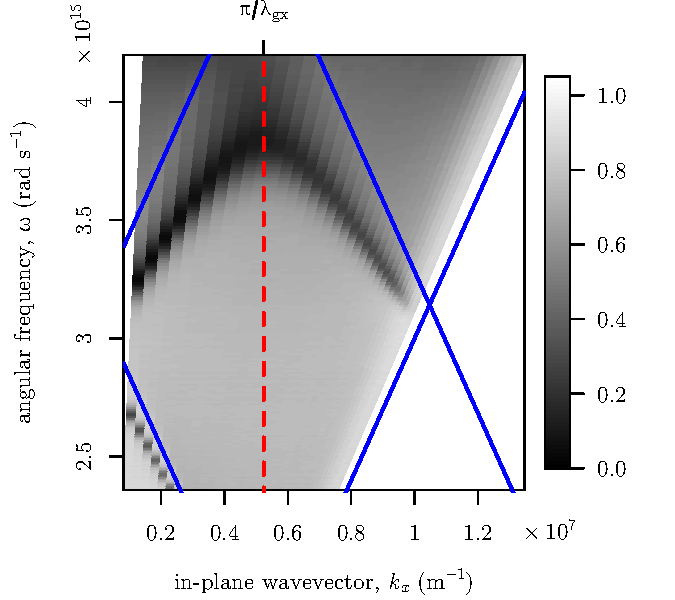
\includegraphics[width=0.49\linewidth]{figure-oblique-RppAtPhi0}}
\subfigure[$R_{TE}$ at $\phi = 75^\circ$]{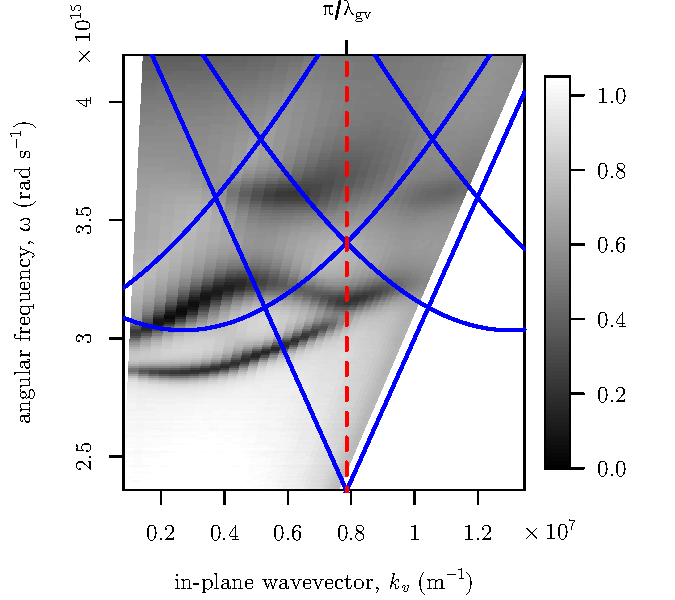
\includegraphics[width=0.49\linewidth]{figure-oblique-RssAtPhi90}}
\end{center}
\caption[Dispersion plots mapped using the reflectivity of an oblique grating.]{Dispersion plots mapped using the reflectivity of an oblique grating, showing the occurrence of band-gaps at the Brillioun Zones along the special cases of (a) $\phi=0^\circ$ and (b) $\phi=75^\circ$.\label{fig:obl-dispersionaroundhighsym}}
\end{figure}
The mid-points of BZ boundaries are of high symmetry in both rectangular and oblique cases (points $i_1,i_2, i_3$ in figure \ref{fig:highsysmpoints-oblique}), and do allow the total cancellation of our vector field. We can observe the points of zero group velocity at these BZ boundaries by mapping the dispersion of the SPP mode in the special cases of $\phi=0^\circ$ and $\phi=75^\circ$, which place the plane of incidence intersecting points $i_1$ and $i_2$ in figure \ref{fig:highsysmpoints-oblique}. In these cases, we fully expect a band-gap to be present at the BZ boundary. These plots are shown in figure \ref{fig:obl-dispersionaroundhighsym}. In the case of of a dispersion diagram such as this, zero group velocity is shown as $\partial \omega/\partial k_{\parallel} = 0$. 

\section{Conclusions}

In this chapter, SPPs propagating on an oblique bigrating have been investigated. The dispersion of these surface modes has been mapped and the SPP interactions discussed in terms of the available scattering amplitudes of the grating. Polarisation conversion is observed on this grating, as SPPs travelling in a direction other than the plane of incidence mediate the rotation of the light's polarisation state.

Using imaging scatterometry, it is observed that the SPP contours are not perturbed as they pass through the conventional BZ boundary. A generalized discussion on the symmetry of the BZ is presented, concluding that this is because the BZ boundary on an oblique grating is not a contour of high symmetry, and only contain isolated points around which the symmetry conditions may be met for the formation of SPP standing waves. Finally, when the plane of incidence intersects these unique points, SPP band gaps may still be observed.


%\begin{sidewaysfigure}
%	\subfigure[][700 nm]{\includegraphics[page=6,width=0.33\textheight ]{scattergrams/figure-700nm-scattergram-withaxes.png}}
%	\subfigure[][650 nm]{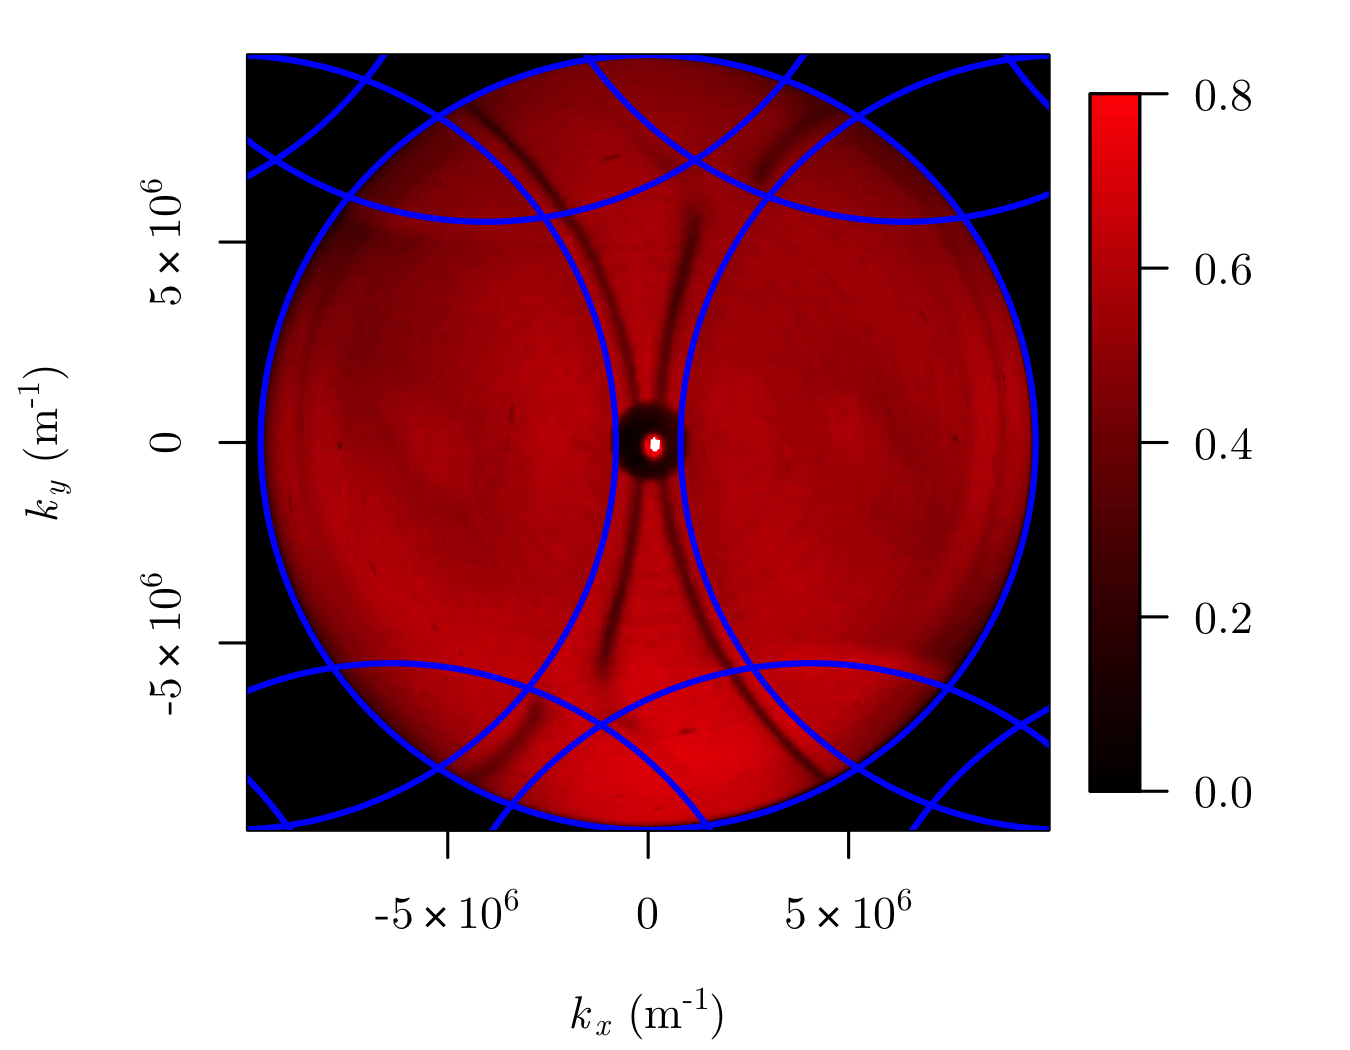
\includegraphics[page=1,width=0.33\textheight]{scattergrams/figure-650nm-scattergram-withaxes.png}}
%	\subfigure[][600 nm]{\includegraphics[page=2,width=0.33\textheight]{scattergrams/figure-600nm-scattergram-withaxes.png}}\\
%	\subfigure[][580 nm]{\includegraphics[page=3,width=0.33\textheight]{scattergrams/figure-580nm-scattergram-withaxes.png}}
%	\subfigure[][550 nm]{\includegraphics[page=4,width=0.33\textheight]{scattergrams/figure-550nm-scattergram-withaxes.png}}
%	\subfigure[][500 nm]{\includegraphics[page=5,width=0.33\textheight]{scattergrams/figure-500nm-scattergram-withaxes.png}}
%
%	\caption{Iso-frequency contours of an oblique grating for a range of wavelengths. The blue circles indicate calculated diffraction edges.}
%\end{sidewaysfigure}


